% Options for packages loaded elsewhere
%DIF LATEXDIFF DIFFERENCE FILE
%DIF DEL hei-report-submitted.tex   Wed Jul 24 11:45:55 2024
%DIF ADD hei-report-revised.tex     Wed Jul 24 14:06:46 2024
\PassOptionsToPackage{unicode}{hyperref}
\PassOptionsToPackage{hyphens}{url}
\PassOptionsToPackage{dvipsnames,svgnames,x11names}{xcolor}
%
\documentclass[
  letterpaper,
  DIV=11,
  numbers=noendperiod]{scrartcl}

\usepackage{amsmath,amssymb}
\usepackage{iftex}
\ifPDFTeX
  \usepackage[T1]{fontenc}
  \usepackage[utf8]{inputenc}
  \usepackage{textcomp} % provide euro and other symbols
\else % if luatex or xetex
  \usepackage{unicode-math}
  \defaultfontfeatures{Scale=MatchLowercase}
  \defaultfontfeatures[\rmfamily]{Ligatures=TeX,Scale=1}
\fi
\usepackage{lmodern}
\ifPDFTeX\else  
    % xetex/luatex font selection
\fi
% Use upquote if available, for straight quotes in verbatim environments
\IfFileExists{upquote.sty}{\usepackage{upquote}}{}
\IfFileExists{microtype.sty}{% use microtype if available
  \usepackage[]{microtype}
  \UseMicrotypeSet[protrusion]{basicmath} % disable protrusion for tt fonts
}{}
\makeatletter
\@ifundefined{KOMAClassName}{% if non-KOMA class
  \IfFileExists{parskip.sty}{%
    \usepackage{parskip}
  }{% else
    \setlength{\parindent}{0pt}
    \setlength{\parskip}{6pt plus 2pt minus 1pt}}
}{% if KOMA class
  \KOMAoptions{parskip=half}}
\makeatother
\usepackage{xcolor}
\usepackage[right=1in,left=1in]{geometry}
\setlength{\emergencystretch}{3em} % prevent overfull lines
\setcounter{secnumdepth}{3}
% Make \paragraph and \subparagraph free-standing
\ifx\paragraph\undefined\else
  \let\oldparagraph\paragraph
  \renewcommand{\paragraph}[1]{\oldparagraph{#1}\mbox{}}
\fi
\ifx\subparagraph\undefined\else
  \let\oldsubparagraph\subparagraph
  \renewcommand{\subparagraph}[1]{\oldsubparagraph{#1}\mbox{}}
\fi


\providecommand{\tightlist}{%
  \setlength{\itemsep}{0pt}\setlength{\parskip}{0pt}}\usepackage{longtable,booktabs,array}
\usepackage{calc} % for calculating minipage widths
% Correct order of tables after \paragraph or \subparagraph
\usepackage{etoolbox}
\makeatletter
\patchcmd\longtable{\par}{\if@noskipsec\mbox{}\fi\par}{}{}
\makeatother
% Allow footnotes in longtable head/foot
\IfFileExists{footnotehyper.sty}{\usepackage{footnotehyper}}{\usepackage{footnote}}
\makesavenoteenv{longtable}
\usepackage{graphicx}
\makeatletter
\def\maxwidth{\ifdim\Gin@nat@width>\linewidth\linewidth\else\Gin@nat@width\fi}
\def\maxheight{\ifdim\Gin@nat@height>\textheight\textheight\else\Gin@nat@height\fi}
\makeatother
% Scale images if necessary, so that they will not overflow the page
% margins by default, and it is still possible to overwrite the defaults
% using explicit options in \includegraphics[width, height, ...]{}
\setkeys{Gin}{width=\maxwidth,height=\maxheight,keepaspectratio}
% Set default figure placement to htbp
\makeatletter
\def\fps@figure{htbp}
\makeatother
%DIF 81a81-91
% definitions for citeproc citations %DIF > 
\NewDocumentCommand\citeproctext{}{} %DIF > 
\NewDocumentCommand\citeproc{mm}{% %DIF > 
  \begingroup\def\citeproctext{#2}\cite{#1}\endgroup} %DIF > 
\makeatletter %DIF > 
 % allow citations to break across lines %DIF > 
 \let\@cite@ofmt\@firstofone %DIF > 
 % avoid brackets around text for \cite: %DIF > 
 \def\@biblabel#1{} %DIF > 
 \def\@cite#1#2{{#1\if@tempswa , #2\fi}} %DIF > 
\makeatother %DIF > 
%DIF -------
\newlength{\cslhangindent}
\setlength{\cslhangindent}{1.5em}
\newlength{\csllabelwidth}
\setlength{\csllabelwidth}{3em}
%DIF 85-89c96-100
%DIF < \newlength{\cslentryspacingunit} % times entry-spacing
%DIF < \setlength{\cslentryspacingunit}{\parskip}
%DIF < \newenvironment{CSLReferences}[2] % #1 hanging-ident, #2 entry spacing
%DIF <  {% don't indent paragraphs
%DIF <   \setlength{\parindent}{0pt}
%DIF -------
\newenvironment{CSLReferences}[2] % #1 hanging-indent, #2 entry-spacing %DIF > 
 {\begin{list}{}{% %DIF > 
  \setlength{\itemindent}{0pt} %DIF > 
  \setlength{\leftmargin}{0pt} %DIF > 
  \setlength{\parsep}{0pt} %DIF > 
%DIF -------
  % turn on hanging indent if param 1 is 1
  \ifodd #1
%DIF 92-93c103-104
%DIF <   \let\oldpar\par
%DIF <   \def\par{\hangindent=\cslhangindent\oldpar}
%DIF -------
   \setlength{\leftmargin}{\cslhangindent} %DIF > 
   \setlength{\itemindent}{-1\cslhangindent} %DIF > 
%DIF -------
  \fi
  % set entry spacing
%DIF 96-98c107-108
%DIF <   \setlength{\parskip}{#2\cslentryspacingunit}
%DIF <  }%
%DIF <  {}
%DIF -------
  \setlength{\itemsep}{#2\baselineskip}}} %DIF > 
 {\end{list}} %DIF > 
%DIF -------
\usepackage{calc}
%DIF 100-102c110-112
%DIF < \newcommand{\CSLBlock}[1]{#1\hfill\break}
%DIF < \newcommand{\CSLLeftMargin}[1]{\parbox[t]{\csllabelwidth}{#1}}
%DIF < \newcommand{\CSLRightInline}[1]{\parbox[t]{\linewidth - \csllabelwidth}{#1}\break}
%DIF -------
\newcommand{\CSLBlock}[1]{\hfill\break#1\hfill\break} %DIF > 
\newcommand{\CSLLeftMargin}[1]{\parbox[t]{\csllabelwidth}{\strut#1\strut}} %DIF > 
\newcommand{\CSLRightInline}[1]{\parbox[t]{\linewidth - \csllabelwidth}{\strut#1\strut}} %DIF > 
%DIF -------
\newcommand{\CSLIndent}[1]{\hspace{\cslhangindent}#1}

\usepackage{booktabs}
\usepackage{longtable}
\usepackage{array}
\usepackage{multirow}
\usepackage{wrapfig}
\usepackage{float}
\usepackage{colortbl}
\usepackage{pdflscape}
\usepackage{tabu}
\usepackage{threeparttable}
\usepackage{threeparttablex}
\usepackage[normalem]{ulem}
\usepackage{makecell}
\usepackage{xcolor}
%DIF 119-128d129
%DIF < \usepackage{siunitx}
%DIF < 
%DIF <   \newcolumntype{d}{S[
%DIF <     input-open-uncertainty=,
%DIF <     input-close-uncertainty=,
%DIF <     parse-numbers = false,
%DIF <     table-align-text-pre=false,
%DIF <     table-align-text-post=false
%DIF <   ]}
%DIF <   
%DIF -------
\usepackage{wrapfig}
\usepackage{colortbl}
 \makeatletter
 \renewenvironment{table}%
   {\renewcommand\familydefault\sfdefault
    \@float{table}}
   {\end@float}
 \renewenvironment{figure}%
   {\renewcommand\familydefault\sfdefault
    \@float{figure}}
   {\end@float}
 \makeatother
%DIF 141a141
\usepackage{changes} %DIF > 
%DIF -------
\KOMAoption{captions}{tableheading}
\makeatletter
%DIF 143-146d144
%DIF < \makeatother
%DIF < \makeatletter
%DIF < \makeatother
%DIF < \makeatletter
%DIF -------
\@ifpackageloaded{caption}{}{\usepackage{caption}}
\AtBeginDocument{%
\ifdefined\contentsname
  \renewcommand*\contentsname{Table of contents}
\else
  \newcommand\contentsname{Table of contents}
\fi
\ifdefined\listfigurename
  \renewcommand*\listfigurename{List of Figures}
\else
  \newcommand\listfigurename{List of Figures}
\fi
\ifdefined\listtablename
  \renewcommand*\listtablename{List of Tables}
\else
  \newcommand\listtablename{List of Tables}
\fi
\ifdefined\figurename
  \renewcommand*\figurename{Figure}
\else
  \newcommand\figurename{Figure}
\fi
\ifdefined\tablename
  \renewcommand*\tablename{Table}
\else
  \newcommand\tablename{Table}
\fi
}
\@ifpackageloaded{float}{}{\usepackage{float}}
\floatstyle{ruled}
\@ifundefined{c@chapter}{\newfloat{codelisting}{h}{lop}}{\newfloat{codelisting}{h}{lop}[chapter]}
\floatname{codelisting}{Listing}
\newcommand*\listoflistings{\listof{codelisting}{List of Listings}}
\makeatother
\makeatletter
%DIF 182-183d179
%DIF < \@ifpackageloaded{caption}{}{\usepackage{caption}}
%DIF < \@ifpackageloaded{subcaption}{}{\usepackage{subcaption}}
%DIF -------
\makeatother
\makeatletter
%DIF 186-193c181-182
%DIF < \@ifpackageloaded{tcolorbox}{}{\usepackage[skins,breakable]{tcolorbox}}
%DIF < \makeatother
%DIF < \makeatletter
%DIF < \@ifundefined{shadecolor}{\definecolor{shadecolor}{rgb}{.97, .97, .97}}
%DIF < \makeatother
%DIF < \makeatletter
%DIF < \makeatother
%DIF < \makeatletter
%DIF -------
\@ifpackageloaded{caption}{}{\usepackage{caption}} %DIF > 
\@ifpackageloaded{subcaption}{}{\usepackage{subcaption}} %DIF > 
%DIF -------
\makeatother
\ifLuaTeX
  \usepackage{selnolig}  % disable illegal ligatures
\fi
\IfFileExists{bookmark.sty}{\usepackage{bookmark}}{\usepackage{hyperref}}
\IfFileExists{xurl.sty}{\usepackage{xurl}}{} % add URL line breaks if available
\urlstyle{same} % disable monospaced font for URLs
\hypersetup{
  pdftitle={How Do Household Energy Transitions Work?},
  pdfauthor={Jill Baumgartner (Co-PI); Sam Harper (Co-PI); On behalf of the Beijing Household Energy Transitions Team},
  colorlinks=true,
  linkcolor={blue},
  filecolor={Maroon},
  citecolor={Blue},
  urlcolor={Blue},
  pdfcreator={LaTeX via pandoc}}

\title{How Do Household Energy Transitions Work?}
\author{Jill Baumgartner (Co-PI) \and Sam Harper (Co-PI) \and On behalf
of the Beijing Household Energy Transitions Team}
\date{\DIFdelbegin \DIFdel{2024-04-27}\DIFdelend \DIFaddbegin \DIFadd{2024-07-24}\DIFaddend }
%DIF PREAMBLE EXTENSION ADDED BY LATEXDIFF
%DIF UNDERLINE PREAMBLE %DIF PREAMBLE
\RequirePackage[normalem]{ulem} %DIF PREAMBLE
\RequirePackage{color}\definecolor{RED}{rgb}{1,0,0}\definecolor{BLUE}{rgb}{0,0,1} %DIF PREAMBLE
\providecommand{\DIFaddtex}[1]{{\protect\color{blue}\uwave{#1}}} %DIF PREAMBLE
\providecommand{\DIFdeltex}[1]{{\protect\color{red}\sout{#1}}}                      %DIF PREAMBLE
%DIF SAFE PREAMBLE %DIF PREAMBLE
\providecommand{\DIFaddbegin}{} %DIF PREAMBLE
\providecommand{\DIFaddend}{} %DIF PREAMBLE
\providecommand{\DIFdelbegin}{} %DIF PREAMBLE
\providecommand{\DIFdelend}{} %DIF PREAMBLE
\providecommand{\DIFmodbegin}{} %DIF PREAMBLE
\providecommand{\DIFmodend}{} %DIF PREAMBLE
%DIF FLOATSAFE PREAMBLE %DIF PREAMBLE
\providecommand{\DIFaddFL}[1]{\DIFadd{#1}} %DIF PREAMBLE
\providecommand{\DIFdelFL}[1]{\DIFdel{#1}} %DIF PREAMBLE
\providecommand{\DIFaddbeginFL}{} %DIF PREAMBLE
\providecommand{\DIFaddendFL}{} %DIF PREAMBLE
\providecommand{\DIFdelbeginFL}{} %DIF PREAMBLE
\providecommand{\DIFdelendFL}{} %DIF PREAMBLE
%DIF HYPERREF PREAMBLE %DIF PREAMBLE
\providecommand{\DIFadd}[1]{\texorpdfstring{\DIFaddtex{#1}}{#1}} %DIF PREAMBLE
\providecommand{\DIFdel}[1]{\texorpdfstring{\DIFdeltex{#1}}{}} %DIF PREAMBLE
\newcommand{\DIFscaledelfig}{0.5}
%DIF HIGHLIGHTGRAPHICS PREAMBLE %DIF PREAMBLE
\RequirePackage{settobox} %DIF PREAMBLE
\RequirePackage{letltxmacro} %DIF PREAMBLE
\newsavebox{\DIFdelgraphicsbox} %DIF PREAMBLE
\newlength{\DIFdelgraphicswidth} %DIF PREAMBLE
\newlength{\DIFdelgraphicsheight} %DIF PREAMBLE
% store original definition of \includegraphics %DIF PREAMBLE
\LetLtxMacro{\DIFOincludegraphics}{\includegraphics} %DIF PREAMBLE
\newcommand{\DIFaddincludegraphics}[2][]{{\color{blue}\fbox{\DIFOincludegraphics[#1]{#2}}}} %DIF PREAMBLE
\newcommand{\DIFdelincludegraphics}[2][]{% %DIF PREAMBLE
\sbox{\DIFdelgraphicsbox}{\DIFOincludegraphics[#1]{#2}}% %DIF PREAMBLE
\settoboxwidth{\DIFdelgraphicswidth}{\DIFdelgraphicsbox} %DIF PREAMBLE
\settoboxtotalheight{\DIFdelgraphicsheight}{\DIFdelgraphicsbox} %DIF PREAMBLE
\scalebox{\DIFscaledelfig}{% %DIF PREAMBLE
\parbox[b]{\DIFdelgraphicswidth}{\usebox{\DIFdelgraphicsbox}\\[-\baselineskip] \rule{\DIFdelgraphicswidth}{0em}}\llap{\resizebox{\DIFdelgraphicswidth}{\DIFdelgraphicsheight}{% %DIF PREAMBLE
\setlength{\unitlength}{\DIFdelgraphicswidth}% %DIF PREAMBLE
\begin{picture}(1,1)% %DIF PREAMBLE
\thicklines\linethickness{2pt} %DIF PREAMBLE
{\color[rgb]{1,0,0}\put(0,0){\framebox(1,1){}}}% %DIF PREAMBLE
{\color[rgb]{1,0,0}\put(0,0){\line( 1,1){1}}}% %DIF PREAMBLE
{\color[rgb]{1,0,0}\put(0,1){\line(1,-1){1}}}% %DIF PREAMBLE
\end{picture}% %DIF PREAMBLE
}\hspace*{3pt}}} %DIF PREAMBLE
} %DIF PREAMBLE
\LetLtxMacro{\DIFOaddbegin}{\DIFaddbegin} %DIF PREAMBLE
\LetLtxMacro{\DIFOaddend}{\DIFaddend} %DIF PREAMBLE
\LetLtxMacro{\DIFOdelbegin}{\DIFdelbegin} %DIF PREAMBLE
\LetLtxMacro{\DIFOdelend}{\DIFdelend} %DIF PREAMBLE
\DeclareRobustCommand{\DIFaddbegin}{\DIFOaddbegin \let\includegraphics\DIFaddincludegraphics} %DIF PREAMBLE
\DeclareRobustCommand{\DIFaddend}{\DIFOaddend \let\includegraphics\DIFOincludegraphics} %DIF PREAMBLE
\DeclareRobustCommand{\DIFdelbegin}{\DIFOdelbegin \let\includegraphics\DIFdelincludegraphics} %DIF PREAMBLE
\DeclareRobustCommand{\DIFdelend}{\DIFOaddend \let\includegraphics\DIFOincludegraphics} %DIF PREAMBLE
\LetLtxMacro{\DIFOaddbeginFL}{\DIFaddbeginFL} %DIF PREAMBLE
\LetLtxMacro{\DIFOaddendFL}{\DIFaddendFL} %DIF PREAMBLE
\LetLtxMacro{\DIFOdelbeginFL}{\DIFdelbeginFL} %DIF PREAMBLE
\LetLtxMacro{\DIFOdelendFL}{\DIFdelendFL} %DIF PREAMBLE
\DeclareRobustCommand{\DIFaddbeginFL}{\DIFOaddbeginFL \let\includegraphics\DIFaddincludegraphics} %DIF PREAMBLE
\DeclareRobustCommand{\DIFaddendFL}{\DIFOaddendFL \let\includegraphics\DIFOincludegraphics} %DIF PREAMBLE
\DeclareRobustCommand{\DIFdelbeginFL}{\DIFOdelbeginFL \let\includegraphics\DIFdelincludegraphics} %DIF PREAMBLE
\DeclareRobustCommand{\DIFdelendFL}{\DIFOaddendFL \let\includegraphics\DIFOincludegraphics} %DIF PREAMBLE
%DIF COLORLISTINGS PREAMBLE %DIF PREAMBLE
\RequirePackage{listings} %DIF PREAMBLE
\RequirePackage{color} %DIF PREAMBLE
\lstdefinelanguage{DIFcode}{ %DIF PREAMBLE
%DIF DIFCODE_UNDERLINE %DIF PREAMBLE
  moredelim=[il][\color{red}\sout]{\%DIF\ <\ }, %DIF PREAMBLE
  moredelim=[il][\color{blue}\uwave]{\%DIF\ >\ } %DIF PREAMBLE
} %DIF PREAMBLE
\lstdefinestyle{DIFverbatimstyle}{ %DIF PREAMBLE
	language=DIFcode, %DIF PREAMBLE
	basicstyle=\ttfamily, %DIF PREAMBLE
	columns=fullflexible, %DIF PREAMBLE
	keepspaces=true %DIF PREAMBLE
} %DIF PREAMBLE
\lstnewenvironment{DIFverbatim}{\lstset{style=DIFverbatimstyle}}{} %DIF PREAMBLE
\lstnewenvironment{DIFverbatim*}{\lstset{style=DIFverbatimstyle,showspaces=true}}{} %DIF PREAMBLE
%DIF END PREAMBLE EXTENSION ADDED BY LATEXDIFF

\begin{document}
\maketitle
\DIFdelbegin %DIFDELCMD < \ifdefined\Shaded\renewenvironment{Shaded}{\begin{tcolorbox}[breakable, borderline west={3pt}{0pt}{shadecolor}, sharp corners, interior hidden, boxrule=0pt, frame hidden, enhanced]}{\end{tcolorbox}}\fi
%DIFDELCMD < 

%DIFDELCMD < %%%
\DIFdelend \renewcommand*\contentsname{Table of contents}
{
\hypersetup{linkcolor=}
\setcounter{tocdepth}{3}
\tableofcontents
}
\DIFdelbegin %DIFDELCMD < \hypertarget{abstract}{%
%DIFDELCMD < \subsection*{Abstract}\label{abstract}}
%DIFDELCMD < %%%
\DIFdelend \DIFaddbegin \subsection*{\DIFadd{Abstract}}\label{abstract}
\DIFaddend 

\DIFdelbegin %DIFDELCMD < \hypertarget{introduction}{%
%DIFDELCMD < \subsubsection*{Introduction}\label{introduction}}
%DIFDELCMD < %%%
\DIFdelend \DIFaddbegin \subsubsection*{\DIFadd{Introduction}}\label{introduction}
\DIFaddend 

Since 2015, thousands of villages across Beijing and northern China have
been treated by a Coal Ban and Heat Pump (CBHP) subsidy policy that
banned household coal burning and subsidized the cost of replacement
with electric heaters and electricity. Whether this large-scale policy
was successful in improving air quality and health remains an important
and unresolved question. We estimated the effects of the CBHP policy on
air quality and cardiopulmonary health in Beijing villages, and
quantified how much of the policy's effects on health were mediated by
changes in air pollution and indoor temperature.

\DIFdelbegin %DIFDELCMD < \hypertarget{methods}{%
%DIFDELCMD < \subsubsection*{Methods}\label{methods}}
%DIFDELCMD < %%%
\DIFdelend \DIFaddbegin \subsubsection*{\DIFadd{Methods}}\label{methods}
\DIFaddend 

In winter 2018-19 we enrolled 1003 participants in 50 Beijing villages
that were eligible for, but not currently treated by, the CBHP policy
and followed them over four consecutive winter data collection waves. In
waves 1, 2 and 4, we administered questionnaires and measured
participants' anthropometrics, blood pressure (BP), airway inflammation
(FeNO), and 24-h personal exposure to fine particulate matter
(PM\textsubscript{2.5}). Fasting whole blood samples were obtained at
clinic visits in waves 1 and 2 for analysis of glucose, lipid profile,
and markers of inflammation and oxidative stress. Wintertime outdoor
PM\textsubscript{2.5} was measured in all 4 waves, and wintertime indoor
temperature and PM\textsubscript{2.5} were measured in waves 2, 3 and 4.
The PM\textsubscript{2.5} filters were analyzed for mass and chemical
composition, which were used for source apportionment. To estimate the
impacts of the policy we used a difference-in-differences design that
accommodated the staggered rollout of the CBHP policy. We used
`extended' two-way fixed effects models and marginal effects to quantify
the effect of the policy on air pollution and health. We further
evaluated whether villages treated by the policy in different years
respond differently to the policy, and if any of the observed health
impacts of the policy were mediated through changes in air pollution or
home (indoor) temperature.

\DIFdelbegin %DIFDELCMD < \hypertarget{results}{%
%DIFDELCMD < \subsubsection*{Results}\label{results}}
%DIFDELCMD < %%%
\DIFdelend \DIFaddbegin \subsubsection*{\DIFadd{Results}}\label{results}
\DIFaddend 

At baseline (wave 1), mean participant age was 60 y (SD=9.2), 60\% were
female, and most (63\%) worked in agriculture. Geometric mean personal
exposures to PM\textsubscript{2.5} were twice as high as outdoor
PM\textsubscript{2.5} (72 versus 36 µg/m\textsuperscript{3}), and the
main source contributors were local and transported dust, regional and
domestic coal and biomass burning, and aerosols that form through
secondary formation. By waves 2, 3, and 4 there were a cumulative total
of 10, 17, and 20 (out of 50 total) villages exposed to the CBHP policy.
Uptake and adherence to the policy was high: among villages treated in
wave 2, the proportion of households using heat pumps and coal heaters,
respectively, changed from 3\% and 97\% in wave 1 to 94\% and 3\% in
wave 4, with similar transitions in villages exposed to the policy in
later waves. Marginal effects derived from multivariable extended
two-way fixed effects models showed that exposure to the policy
increased indoor temperature by 1-2°C and reduced indoor seasonal
PM\textsubscript{2.5} by approximately 36 µg/m\textsuperscript{3}.
Exposure to the policy also reduced contributions to
PM\textsubscript{2.5} from solid fuel sources, including household coal
burning, and improved blood pressure (\textasciitilde1.5 mmHg lower
systolic and diastolic) and self-reported respiratory symptoms
(\textasciitilde7 percentage point reduction in any symptoms). There was
notable heterogeneity in effects across treatment cohorts, with larger
benefits to indoor PM\textsubscript{2.5} and health in villages treated
in earlier relative to later years. In the mediation analysis, indoor
PM\textsubscript{2.5} and indoor temperature explained most of the total
effect of the policy on systolic BP and roughly half of the total effect
on diastolic BP, but did not explain improvements in self-reported
respiratory symptoms. The policy did not show evidence of meaningful
effects on outdoor or personal exposure to PM\textsubscript{2.5}, or on
biomarkers of inflammation and oxidative stress.

\DIFdelbegin %DIFDELCMD < \hypertarget{conclusions}{%
%DIFDELCMD < \subsubsection*{Conclusions}\label{conclusions}}
%DIFDELCMD < %%%
\DIFdelend \DIFaddbegin \subsubsection*{\DIFadd{Conclusions}}\label{conclusions}
\DIFaddend 

In this comprehensive field-based assessment of a real-world household
energy policy in Beijing, we observed high fidelity and compliance with
the CBHP policy. Exposure to the policy reduced blood pressure and
self-reported chronic respiratory symptoms, and the effects for blood
pressure were mediated by reductions in indoor PM\textsubscript{2.5} and
improvements in home temperature, providing empirical evidence that
clean energy policies can provide population health benefits.

\newpage

\DIFdelbegin %DIFDELCMD < \hypertarget{introduction-1}{%
%DIFDELCMD < \section{Introduction}\label{introduction-1}}
%DIFDELCMD < %%%
\DIFdelend \DIFaddbegin \section{\DIFadd{Introduction}}\label{introduction-1}
\DIFaddend 

China is deploying an ambitious policy to transition up to 70\% of
households in northern China from residential coal heating to electric
or gas ``clean'' space heating, including a large-scale roll out across
rural and peri-urban Beijing, referred to in this document as China's
Coal Ban and Heat Pump (CBHP) subsidy policy. To meet this target the
Beijing municipal government announced a two-pronged program that
designates coal-restricted areas and simultaneously offers subsidies to
night-time electricity rates and for the purchase and installation of
electric-powered heat pumps to replace traditional coal-heating stoves.
The policy was piloted in 2015 and, starting in 2016, was rolled out on
a village-by-village basis. The variability in when the policy was
applied to each village allowed us to treat the roll-out of the program
as a quasi-randomized intervention and evaluate its impacts on air
quality and health. Household air pollution is a well-established risk
factor for adverse health outcomes over the entire lifecourse, yet there
is no consensus that clean energy interventions can improve these health
outcomes based on evidence from randomized trials (Lai et al. 2024).
Households may be differentially affected by the CBHP due to factors
such as financial constraints and user preferences, and there is
uncertainty about whether and how the policy may affect indoor and
outdoor air pollution, as well as heating behaviors and health outcomes.

\DIFdelbegin %DIFDELCMD < \hypertarget{background}{%
%DIFDELCMD < \section{Background}\label{background}}
%DIFDELCMD < %%%
\DIFdelend \DIFaddbegin \section{\DIFadd{Background}}\label{background}
\DIFaddend 

\DIFdelbegin %DIFDELCMD < \hypertarget{context-for-the-policy}{%
%DIFDELCMD < \subsection{Context for the policy}\label{context-for-the-policy}}
%DIFDELCMD < %%%
\DIFdelend \DIFaddbegin \subsection{\DIFadd{Context for the policy}}\label{context-for-the-policy}
\DIFaddend 

Beijing has a temperate continental monsoon climate that is
characterized by cold, dry winters and hot, humid summers. Access to
central heating is limited to urban areas and thus most peri-urban and
rural households have historically heated their homes using coal heaters
and biomass \emph{kangs} (a traditional Chinese energy technology that
integrates at least four different home functions including cooking, a
bed for sleeping, space heating, and home ventilation). Household coal
burning was a major contributor to indoor and outdoor air pollution in
northern China, especially in winter. Prior to the CBHP policy, over 100
million rural households consumed \textasciitilde200 million tons of
coal to meet more than 80\% of northern China's residential space
heating demand (Dispersed Coal Management Research Group 2023), which
contributed to roughly 30\% of wintertime air pollution (GBD MAPS
Working Group 2016). In 2013, coal combustion from industrial,
electricity, and residential heating sources was the single largest
estimated contributor to population exposure to PM\textsubscript{2.5} in
China and responsible for an estimated 366,000 annual premature deaths
(GBD MAPS Working Group 2016).

Banning residential coal burning and providing homes with clean heating
alternatives through the CBHP policy was considered a potentially
important intervention to improve rural development, reduce local and
regional PM\textsubscript{2.5}, and mitigate air pollution-related
health impacts. A number of clean heating options, including electric
heat pumps, gas heaters, and electric resistance heaters with thermal
storage, were widely promoted by the Chinese government (Dispersed Coal
Management Research Group 2023). By 2021, over 36 million households in
northern China were treated by the CBHP policy and an estimated 21
million additional households are expected to be treated by 2025.
Whether this large-scale energy policy yielded air quality and health
benefits remains a critical and unresolved question.

\DIFdelbegin %DIFDELCMD < \hypertarget{prior-evidence-on-household-energy-interventions-and-air-pollution}{%
%DIFDELCMD < \subsection{Prior evidence on household energy interventions and air
%DIFDELCMD < pollution}\label{prior-evidence-on-household-energy-interventions-and-air-pollution}}
%DIFDELCMD < %%%
\DIFdelend \DIFaddbegin \subsection{\DIFadd{Prior evidence on household energy interventions and air
pollution}}\label{prior-evidence-on-household-energy-interventions-and-air-pollution}
\DIFaddend 

Household energy interventions, mostly cooking-related, that replace
traditional solid fuel stoves with more efficient and less-polluting
alternatives have been implemented and studied extensively in countries
including China over the past several decades. While the introduction of
cleaner household stoves is expected to reduce air pollution, their
real-world effectiveness in achieving health-relevant air pollution
reductions is unclear (Quansah et al. 2017). In particular, the indoor
and local air quality benefits of large-scale household energy programs
like the CBHP subsidy policy have been rarely empirically investigated,
especially at a sub-city spatial resolution. In Ireland, county-level
residential coal bans in the 1990s were associated with 40-70\%
decreases in black smoke concentrations in ban-affected areas (Dockery
et al. 2013). In Australia, a wood-burning stove exchange lowered daily
wintertime PM\textsubscript{10} from 44 to 27 µg/m\textsuperscript{3}
(Johnston et al. 2013), and clean energy policies in New Zealand were
associated with 11-36\% reductions in winter PM\textsubscript{10} (Scott
and Scarrott 2011). The few evaluations of the CBHP policy reported
small decreases in outdoor PM\textsubscript{2.5} (-7 to -2.4
µg/m\textsuperscript{3}) in municipalities or prefectures treated by the
policy compared with untreated neighboring regions (Niu et al. 2024;
Song et al. 2023; Tan et al. 2023; Yu et al. 2021), and a recent
modeling study estimated 36\% lower personal exposure to
PM\textsubscript{2.5} based on household-reported changes in fuel use
(Meng et al. 2023). However, none of these studies included field-based
measurements of air pollution or personal exposures, which are known to
differ considerably from from modelled estimates based on assumptions of
emissions reductions (Thompson et al. 2019), and few accounted for
secular changes in air quality over time, limiting any conclusions about
the causal effect of the policy on air quality.

\DIFdelbegin %DIFDELCMD < \hypertarget{prior-evidence-on-clean-energy-interventions-and-cardiovascular-outcomes}{%
%DIFDELCMD < \subsection{Prior evidence on clean energy interventions and
%DIFDELCMD < cardiovascular
%DIFDELCMD < outcomes}\label{prior-evidence-on-clean-energy-interventions-and-cardiovascular-outcomes}}
%DIFDELCMD < %%%
\DIFdelend \DIFaddbegin \subsection{\DIFadd{Prior evidence on clean energy interventions and
cardiovascular
outcomes}}\label{prior-evidence-on-clean-energy-interventions-and-cardiovascular-outcomes}
\DIFaddend 

Most previous health assessments of household energy interventions have
focused on cookstoves rather than heating technologies, though in many
settings cookstoves are also used for space heating. Randomized trials
of less polluting cookstoves generally indicate a cardiovascular
benefit. In older Guatemalan women, a chimney stove intervention lowered
exposure to air pollution and reduced the occurrence of nonspecific
ST-segment depression (McCracken et al. 2011). Randomized trials in
Guatemala, Nigeria, and Ghana also showed reductions in blood pressure
(systolic range: \DIFdelbegin \DIFdel{−3.7 to −1.3 }\DIFdelend \DIFaddbegin \DIFadd{-3.7 to -1.3 }\DIFaddend mmHg) in women assigned to gas, ethanol,
or improved combustion biomass stoves. In contrast, recent single
country (Peru) and large multi-country (Household Air Pollution
Intervention Network, HAPIN) trials found no benefit of LPG stoves on
blood pressure (Checkley et al. 2021; Ye et al. 2022) despite much
larger reductions (\textasciitilde66\% lower) in exposure to
PM\textsubscript{2.5} and black carbon than what was observed in trials
showing a BP benefit of intervention (Johnson et al. 2022).

The few population-based evaluations of residential energy policies also
suggest a cardio-respiratory benefit of clean energy transition.
Residential wood-burning bans were associated with reductions in
cardiovascular hospitalizations (-7\%) in California (Yap and Garcia
2015) and with reduced cardiovascular (-17.9\%) and respiratory
(−22.8\%) mortality in Australia (Johnston et al. 2013), though neither
study fully controlled for secular changes in health that were unrelated
to the policy. Most relevant to our study are two quasi-experimental
assessments of coal replacement policies. In Ireland, reductions in
respiratory not but cardiovascular mortality were observed following a
coal ban (Dockery et al. 2013). A multi-city study of Chinese adults in
cities where the CBHP policy was piloted compared with adults in cities
not in the pilot observed small decreases in chronic lung diseases (-3.0
to -1.1\%) but no change in physician-diagnosed cardiovascular diseases,
potentially due to the short (one-year) post-policy evaluation period or
confounding by other unmeasured city-wide air quality or health-related
policies (Wen et al. 2023).

Though household air pollution is a well-established health risk factor,
which energy interventions can reduce air pollution exposures, improve
health, and are scalable and sustainable remains a critical and
unanswered question. In a recent Official American Thoracic Society
Statement, for example, the committee did not reach a consensus that
household energy interventions (including gas, ethanol, solar, and
improved biomass cookstoves) improved health outcomes (including
respiratory symptoms and blood pressure), with 55\% saying no and 45\%
saying yes (Lai et al. 2024).

\DIFdelbegin %DIFDELCMD < \hypertarget{evaluating-the-mechanisms-through-which-policies-may-affect-health-outcomes.}{%
%DIFDELCMD < \subsection{Evaluating the mechanisms through which policies may affect
%DIFDELCMD < health
%DIFDELCMD < outcomes.}\label{evaluating-the-mechanisms-through-which-policies-may-affect-health-outcomes.}}
%DIFDELCMD < %%%
\DIFdelend \DIFaddbegin \subsection{\DIFadd{Evaluating the mechanisms through which policies may affect
health
outcomes.}}\label{evaluating-the-mechanisms-through-which-policies-may-affect-health-outcomes.}
\DIFaddend 

With several exceptions (Alexander et al. 2018; Gould et al. 2023;
McCracken et al. 2007; McCracken et al. 2011), decades of household
energy intervention studies have shown limited or no health benefit,
which demonstrates the complexity of evaluating interventions on
exposures like cooking or space heating that are central to daily life
(Ezzati and Baumgartner 2017; Lai et al. 2024). Energy interventions and
policies, particularly those implemented at the household- or
village-scales, can produce multiple behavioral, environmental, and
health-related changes, making it important to investigate the
mechanisms through which such policies exert their health impacts or
lack of impacts (Dominici et al. 2014). The health benefits achievable
with transition from traditional coal stoves to a new electric home
heating system, for example, may be influenced by factors including
outdoor air quality (Lai 2019), the desirability and usage patterns of
new and traditional stoves (Ezzati and Baumgartner 2017), indoor
temperature (Lewington et al. 2012), or behaviors including physical
activity (Lindemann et al. 2017). Only recently were such mediating
factors considered in health assessments of household energy
interventions, and rarely in a comprehensive or formalized way
(Rosenthal et al. 2018). Understanding such mechanisms can provide
valuable insights into the success (or failure) of clean energy programs
or policies like the CBHP in meeting their air quality and health
targets, and may answer questions that can inform the design of more
effective future energy interventions (Lai et al. 2024). For example, is
there successful uptake of the intervention or policy? Does the policy
lead to heating behavior changes that result in colder homes which may
offset any cardiovascular-enhancing effects of improved air quality?
Answers to these questions are facilitated by the analysis of mediating
pathways, a key aim of this study.

\DIFdelbegin %DIFDELCMD < \hypertarget{specific-aims-and-overarching-approach}{%
%DIFDELCMD < \section{Specific Aims and Overarching
%DIFDELCMD < Approach}\label{specific-aims-and-overarching-approach}}
%DIFDELCMD < %%%
\DIFdelend \DIFaddbegin \section{\DIFadd{Specific Aims and Overarching
Approach}}\label{specific-aims-and-overarching-approach}
\DIFaddend 

We used three data collection waves in winter 2018/19, winter 2019/20,
and winter 2021/22, as well as a partial wave in winter 2020/21 to
advance the following aims:

\begin{enumerate}
\def\labelenumi{\arabic{enumi}.}
\item
  Estimate how much of the CBHP policy's overall effect on health,
  including respiratory symptoms and cardiovascular outcomes (blood
  pressure, blood inflammatory and oxidative stress markers), can be
  attributed to its impact on changes in PM\textsubscript{2.5};
\item
  Quantify the impact of the policy on outdoor air quality and personal
  air pollution exposures, and specifically the source contribution from
  household coal burning;
\item
  Quantify the contribution of changes in the chemical composition of
  PM\textsubscript{2.5} from different sources to the overall effect on
  health outcomes.
\end{enumerate}

\DIFdelbegin %DIFDELCMD < \hypertarget{study-design-and-methods}{%
%DIFDELCMD < \section{Study Design and Methods}\label{study-design-and-methods}}
%DIFDELCMD < %%%
\DIFdelend \DIFaddbegin \section{\DIFadd{Study Design and Methods}}\label{study-design-and-methods}
\DIFaddend 

\DIFdelbegin %DIFDELCMD < \hypertarget{study-area}{%
%DIFDELCMD < \subsection{Study area}\label{study-area}}
%DIFDELCMD < %%%
\DIFdelend \DIFaddbegin \subsection{\DIFadd{Study area}}\label{study-area}
\DIFaddend 

Beijing is the capital of China (pop. 21.9 million in 2020) and covers a
large geographic area (\textasciitilde16,000 km\textsuperscript{2}) that
includes a highly developed and densely-populated urban core that is
surrounded by several satellite towns and thousands of peri-urban and
rural villages in the periphery. Beijing winters begin in early November
and tend to be cold, dry, and windy, with the lowest temperatures most
often occurring in January (-3°C, on average), thus requiring space
heating (An et al. 2021). Most urban areas of Beijing are connected to a
central heating grid that supplies home heating from central locations,
whereas rural and many peri-urban areas have historically relied on
individual space heating units that, prior to 2015, were largely fueled
by unprocessed coal (Duan et al. 2014).

\DIFdelbegin %DIFDELCMD < \hypertarget{location-and-participant-recruitment-and-enrolment}{%
%DIFDELCMD < \subsection{Location and participant recruitment and
%DIFDELCMD < enrolment}\label{location-and-participant-recruitment-and-enrolment}}
%DIFDELCMD < %%%
\DIFdelend \DIFaddbegin \subsection{\DIFadd{Location and participant recruitment and
enrolment}}\label{location-and-participant-recruitment-and-enrolment}
\DIFaddend 

Between December 2018 and January 2019 we recruited 50 villages across 4
administrative districts (Fangshan, Huairou, Mentougou, and Miyun) in
the Beijing municipality in northern China. The villages predominately
used coal for heating at the time of enrollment and were eligible for
but not currently participating in the CBHP policy. Roughly half of the
villages were expected to enter into the policy during our study
(Figure~\ref{fig-cbhp-map}). We used local guides in each village to
help determine a roster of households that were not vacant during the
winter months, from which we randomly selected households to recruit for
participation.

\begin{figure}[H]

\DIFdelbeginFL %DIFDELCMD < {\centering 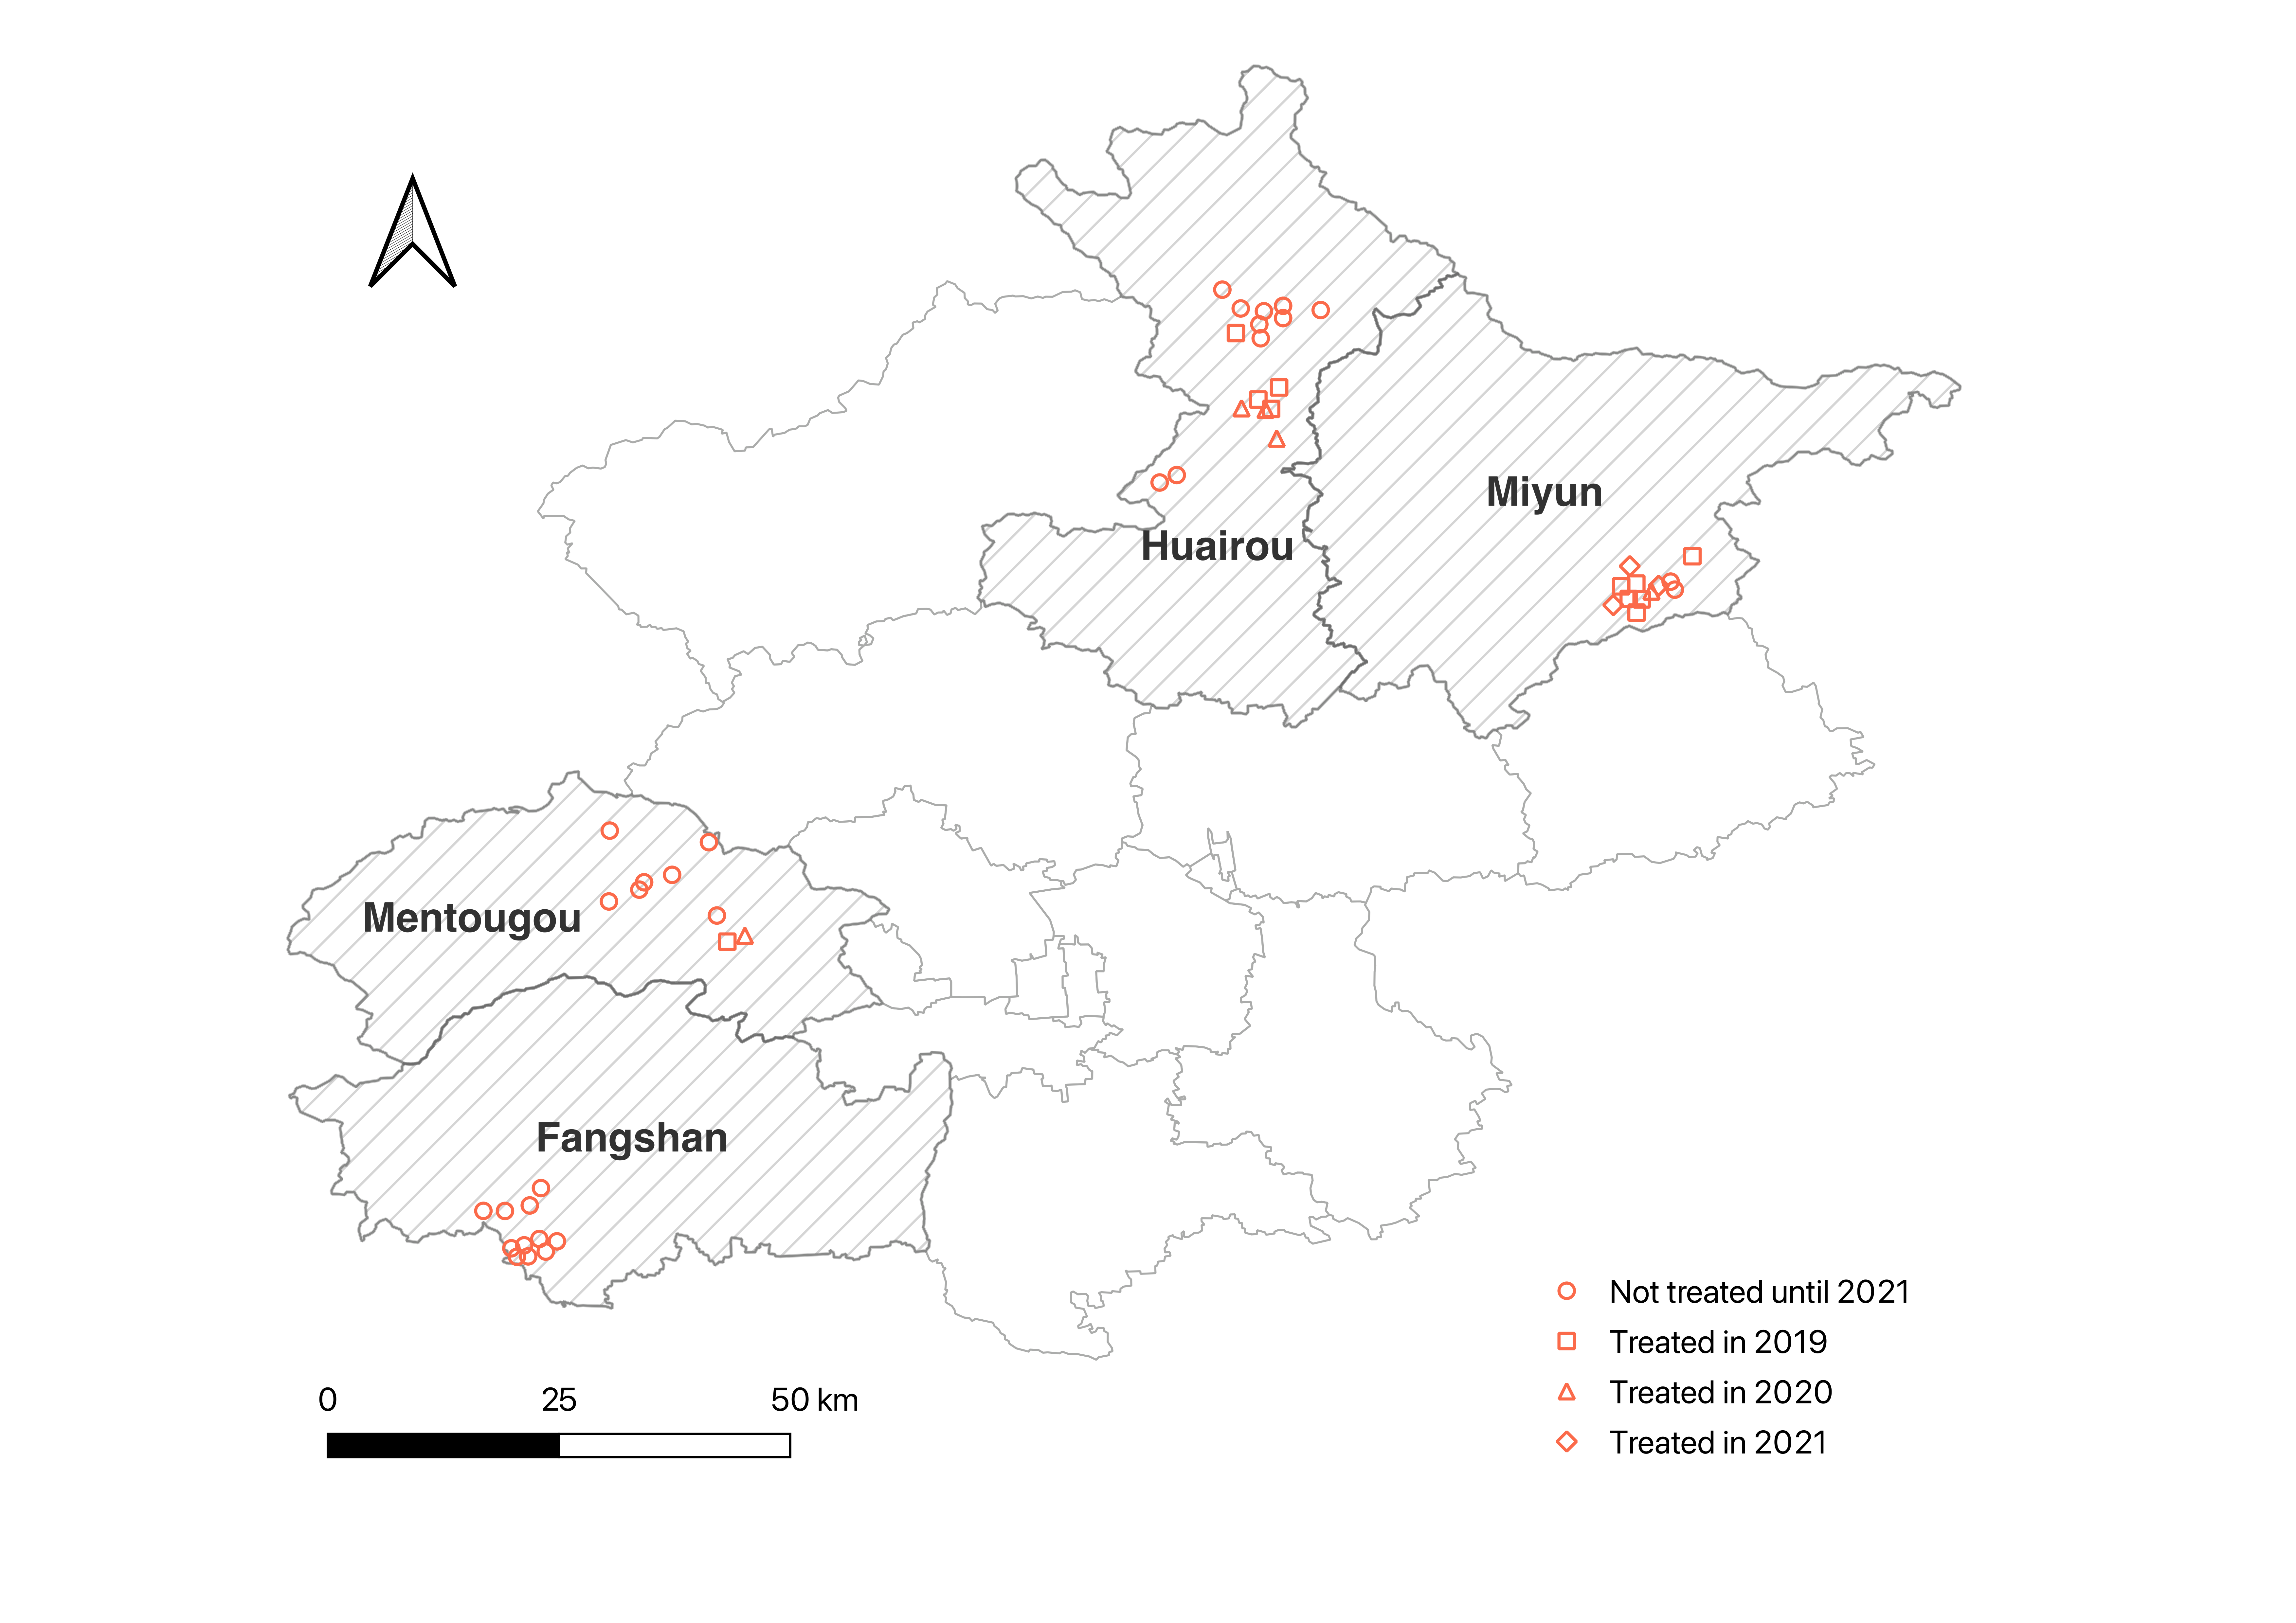
\includegraphics[width=0.7\textwidth,height=\textheight]{images/policy-implementation-map.png}
%DIFDELCMD < %%%
\DIFdelendFL \DIFaddbeginFL \centering{

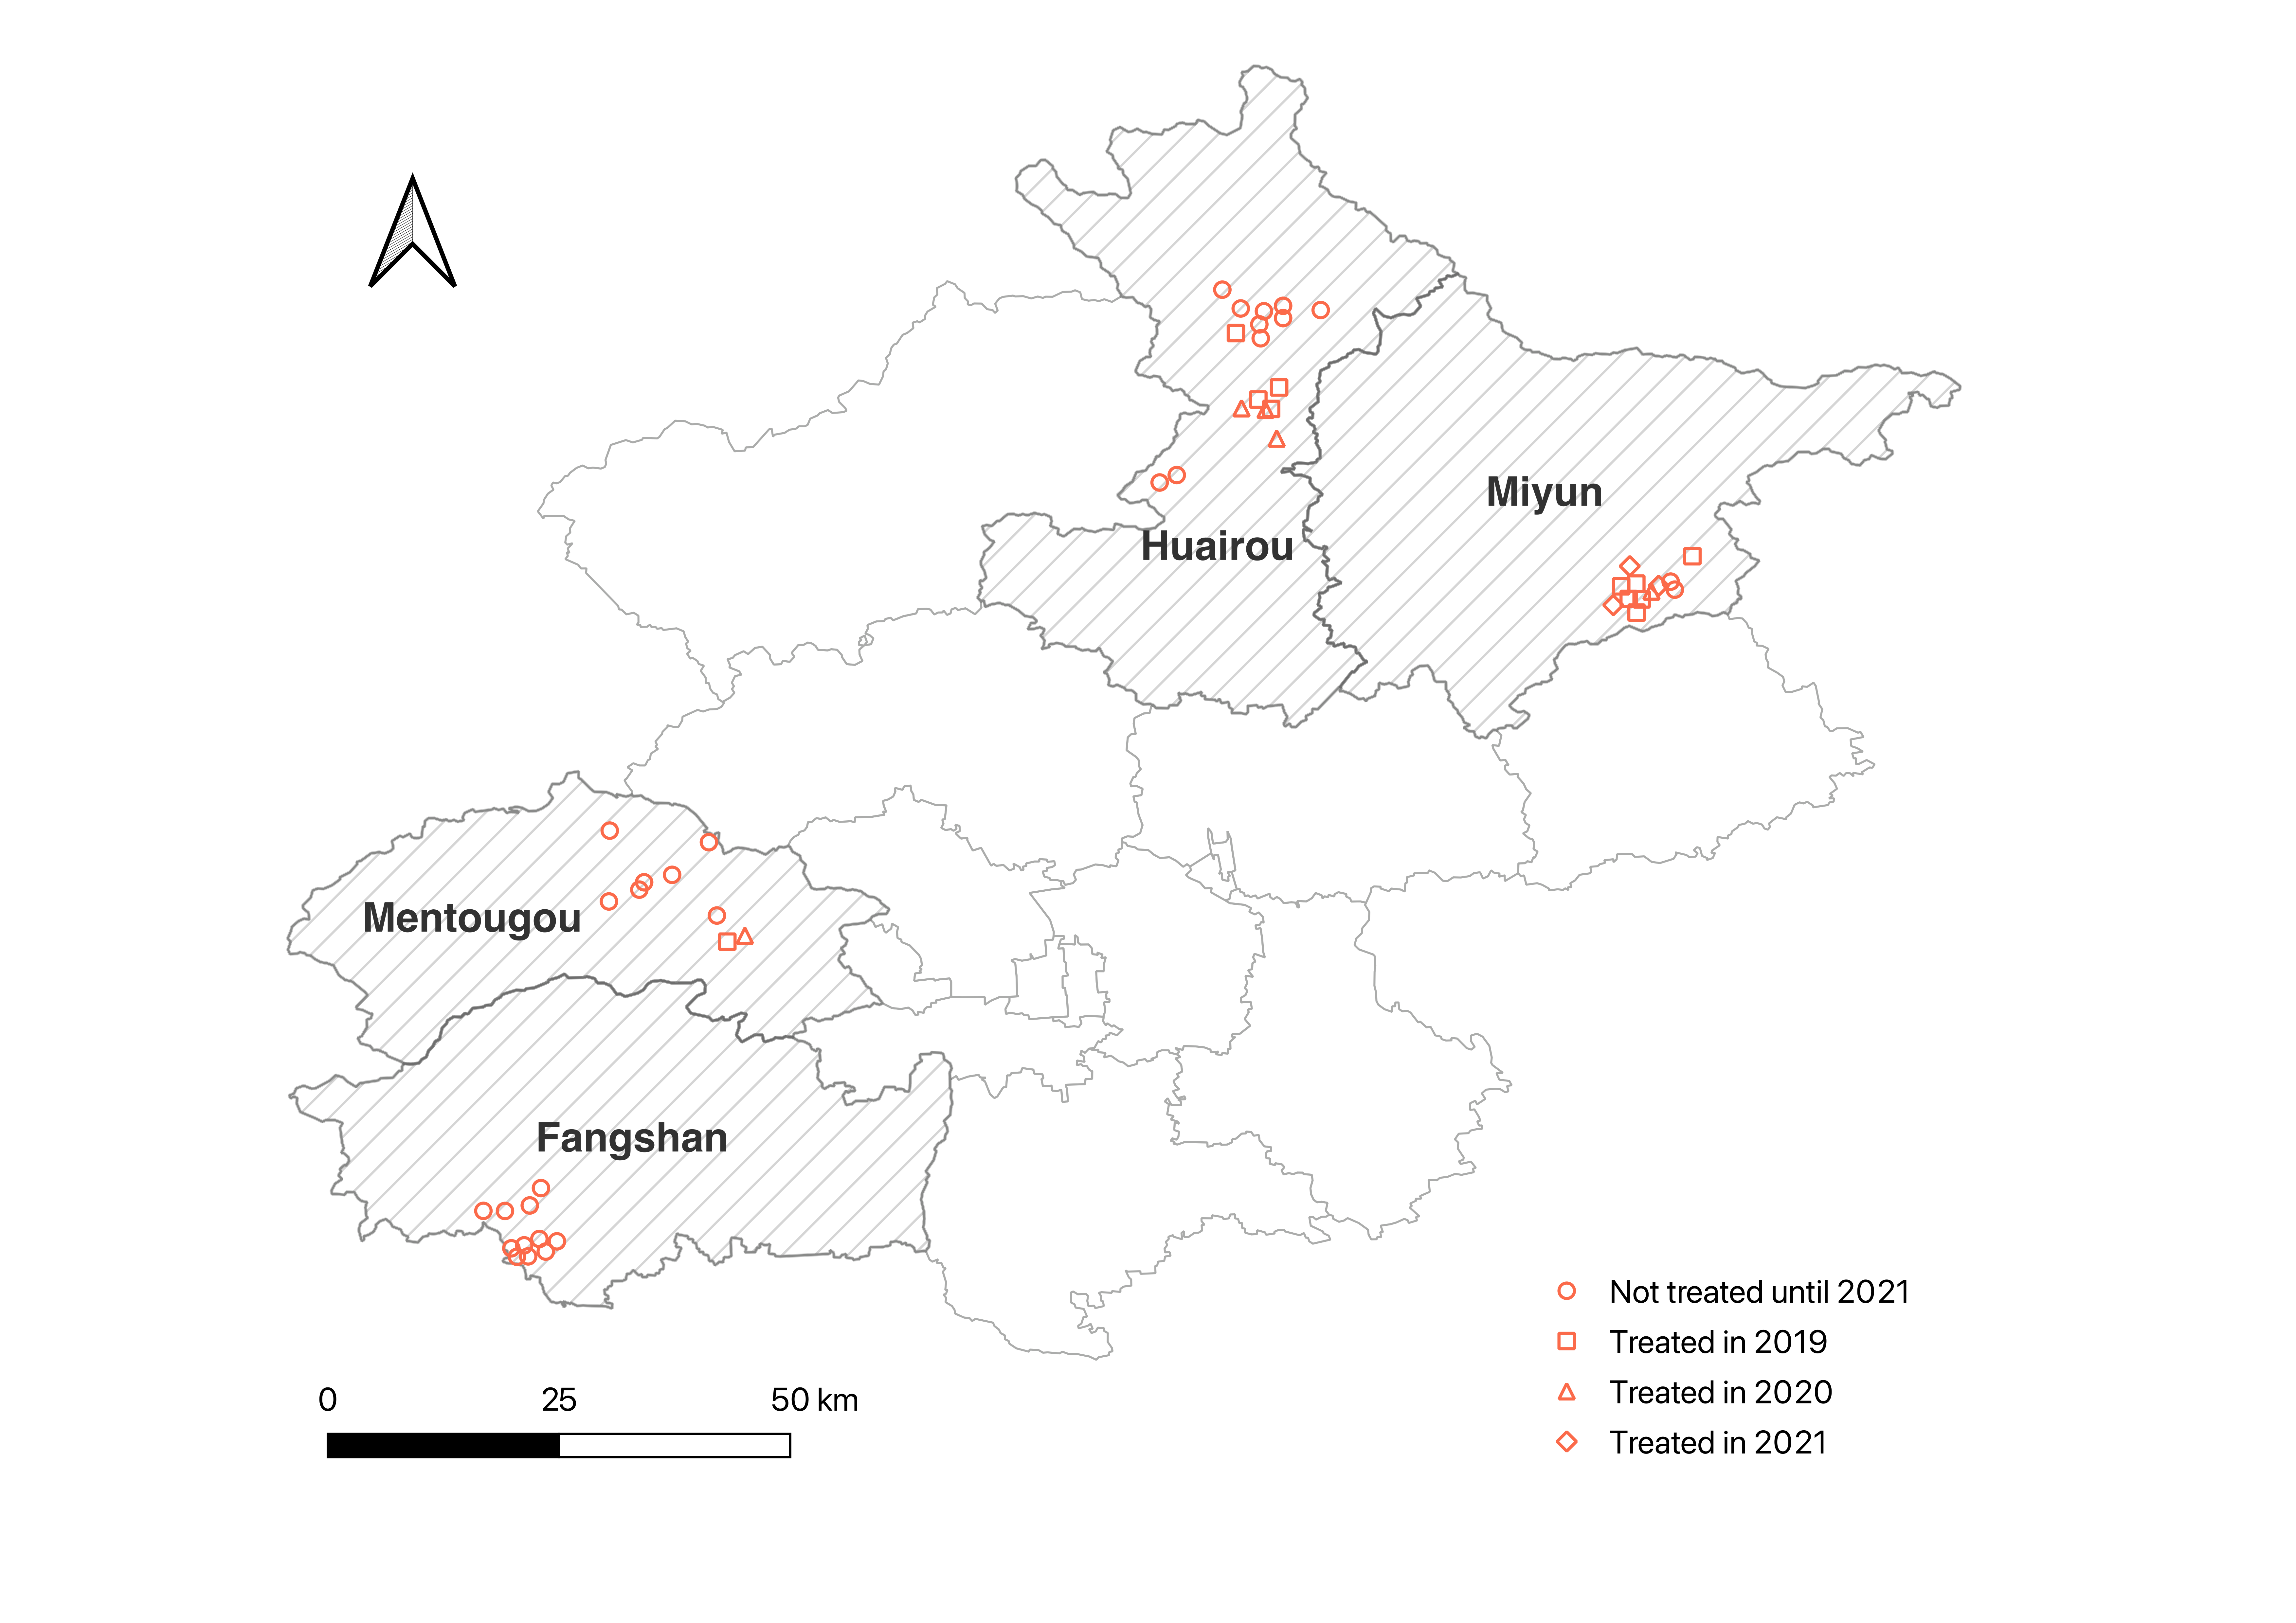
\includegraphics[width=0.7\textwidth,height=\textheight]{images/policy-implementation-map.png}

}
\DIFaddendFL 

\DIFdelbeginFL %DIFDELCMD < }
%DIFDELCMD < 

%DIFDELCMD < %%%
\DIFdelendFL \caption{\label{fig-cbhp-map}Map of village implementation of CBHP
policy}

\end{figure}%DIF > 

We recruited approximately 20 households in each village and randomly
selected one eligible person from each household to participate.
Household members were eligible to participate if they were over 40
years old, lived in the study villages, were not planning to move out of
the village in the next year, and were not on current immunotherapy or
treatment with corticosteroids. Research staff introduced the study and
its measurements to an eligible adult in each household and answered any
questions related to the study. In follow-up visits to the study
villages, staff first approached households with participants from an
earlier wave. If previous participants were not at home or refused to
participate, staff first tried to randomly recruit an eligible
participant from the same household. If there was not another eligible
or willing participant in the household, we randomly selected and
recruited a participant from a new household using the village roster.
All participants provided written informed consent prior to joining the
study. The study protocols were approved by research ethics boards at
Peking University (IRB00001052-18090), Peking Union Medical College
Hospital (HS-3184) and McGill University (A08-E53-18B).

\DIFdelbegin %DIFDELCMD < \hypertarget{data-collection-overview}{%
%DIFDELCMD < \subsection{Data Collection Overview}\label{data-collection-overview}}
%DIFDELCMD < %%%
\DIFdelend \DIFaddbegin \subsection{\DIFadd{Data Collection Overview}}\label{data-collection-overview}
\DIFaddend 

We conducted study measurements over four consecutive waves of data
collection in winter 2018-19, 2019-20, 2020-21, and 2021-22 (referred to
hereafter as Wave 1 {[}w1{]}, w2, w3 and w4, respectively). Field data
collection was conducted by \textasciitilde20 trained staff members who
traveled to participants' homes to conduct tablet-based household and
individual questionnaires, measure participant blood pressure, and
distribute temperature sensors (for measurement of indoor temperature
and stove use) and air pollution monitors in all 50 study villages in
w1, w2, and w4. Anthropometrics (height, weight, and waist
circumference), measurement of airway inflammation, and whole blood
samples were obtained no more than a month later at a village clinic in
w1 and w2. In w3, which was during the height of the COVID-19 pandemic,
we limited household measurements to indoor air quality and sensor-based
measurement of indoor temperature and stove use in 41 villages,
including all 17 treated villages and 24 untreated villages, prior to
COVID-19-related travel restrictions that halted field data collection.
In w4, which also occurred during the COVID-19 pandemic, we returned to
conducting individual-level assessments. However, unlike in w1 and w2,
anthropometric measurements and airway inflammation were assessed in
participant homes rather than clinics to avoid group contact, and blood
samples were not collected. Outdoor (community) air pollution was
measured throughout the study period.

\DIFdelbegin %DIFDELCMD < \hypertarget{air-pollution}{%
%DIFDELCMD < \subsubsection{Air Pollution}\label{air-pollution}}
%DIFDELCMD < %%%
\DIFdelend \DIFaddbegin \subsubsection{\DIFadd{Air Pollution}}\label{air-pollution}
\DIFaddend 

\DIFdelbegin %DIFDELCMD < \hypertarget{outdoor-air-pollution}{%
%DIFDELCMD < \paragraph{Outdoor air pollution}\label{outdoor-air-pollution}}
%DIFDELCMD < %%%
\DIFdelend \DIFaddbegin \paragraph{\DIFadd{Outdoor air pollution}}\label{outdoor-air-pollution}
\DIFaddend 

In each village, two sensors for particulate matter air pollution were
set up to measure outdoor (community) PM\textsubscript{2.5} at different
locations in each village. One sensor was placed near the center of the
village, and the other was placed no less than 500m away from the
centrally-located sensor. Sensors were placed at least 1.5m above the
ground and not in a location within sight of a visible point source of
PM\textsubscript{2.5}.

We collected filter-based community PM\textsubscript{2.5} samples to
calibrate the sensor-based PM\textsubscript{2.5} measurements as well as
to conduct analysis of chemical composition for source apportionment.
Ultrasonic Personal Aerosol Samplers (UPAS, Access Sensor Technologies,
Fort Collins, CO, USA) were used to collect filter-based
PM\textsubscript{2.5} samples with a flow rate of 1.0 L/min (Volckens et
al. 2017). Samplers housed 37mm PTFE filters (VWR, 2.0µm pore size) and
were equipped with a cyclone inlet with a 2.5µm cut point designed to
perform under the sampling flow rate. For community measurements, a UPAS
was co-located with each PM\textsubscript{2.5} sensor in each village in
rotation. Every week, the used filters were removed and replaced with a
new filter. In total, we successfully collected 126, 371, and 289
filter-based, community outdoor PM\textsubscript{2.5} samples in w1, w2,
and w4, respectively. Field blank filters were collected at a rate of
\textasciitilde10\%, subject to the same field conditions as samples. To
support post-sampling determination of organic carbon (OC) and elemental
carbon (EC) fractions of PM\textsubscript{2.5} mass, quartz filters were
co-located with a subset of Teflon filter samples collected outdoors.
Quartz filter-based PM\textsubscript{2.5} samples were collected using
UPAS operating with a flow rate of 1.0 L/min. UPASs housed 37 mm quartz
filters (VWR, 2.0-µm pore size) and were equipped with a cyclone inlet
with a 2.5µm cut point designed to perform under the corresponding
sampling flow rate. All quartz fiber filters were baked at 550 °C for a
minimum of 8 h to remove organic impurities prior to sample collection.
PM\textsubscript{2.5} samples collected on quartz filters were analyzed
using established thermo-optical methods for quantifying elemental
carbon (EC) and organic carbon (OC) to, then, calibrate the colorimetric
analysis of EC and OC on Teflon filters. In w2, 23 quartz-based outdoor
PM\textsubscript{2.5} samples and 3 field blanks were collected. In w4,
11 quartz-based outdoor PM\textsubscript{2.5} samples and 3 field blanks
were collected.

For PM\textsubscript{2.5} sensor calibration and quality control, all PM
sensors were co-located with a reference-grade PM\textsubscript{2.5}
instrument (Model 5030 Synchronized Hybrid Ambient Realtime Particulate
(SHARP) Monitor, Thermo Fisher Scientific, United States) on the rooftop
of a building at Peking University campus and/or the Tapered Element
Oscillating Microbalance (TEOM, Thermo Scientific™ 1405 TEOM™) at the
Chinese Academy of Sciences University campus for 7 to 10 days before
and after each field wave (Figure~\ref{fig-calibration}).
Sensor-measured PM\textsubscript{2.5} concentrations were highly
correlated with those measured by the reference instruments (Spearman
correlation coefficients (rho) \textgreater0.75 in each pre- and
post-calibration).

\begin{figure}[H]

\DIFdelbeginFL %DIFDELCMD < {\centering \includegraphics[width=0.8\textwidth,height=\textheight]{images/sensor-calibration.png}
%DIFDELCMD < %%%
\DIFdelendFL \DIFaddbeginFL \centering{

\includegraphics[width=0.8\textwidth,height=\textheight]{images/sensor-calibration.png}

}
\DIFaddendFL 

\DIFdelbeginFL %DIFDELCMD < }
%DIFDELCMD < 

%DIFDELCMD < %%%
\DIFdelendFL \caption{\label{fig-calibration}Calibration of real-time sensors against
a reference monitor at University of the Chinese Academy of Sciences.}

\end{figure}%DIF > 

\DIFdelbegin %DIFDELCMD < \hypertarget{indoor-pm2.5}{%
%DIFDELCMD < \paragraph{\texorpdfstring{Indoor
%DIFDELCMD < PM\textsubscript{2.5}}{Indoor PM2.5}}\label{indoor-pm2.5}}
%DIFDELCMD < %%%
\DIFdelend \DIFaddbegin \paragraph{\texorpdfstring{Indoor
PM\textsubscript{2.5}}{Indoor PM2.5}}\label{indoor-pm2.5}
\DIFaddend 

In the second, third, and fourth data collection waves we randomly
selected six households from the 20 recruited in each village to measure
indoor concentrations of PM\textsubscript{2.5}. In w4, we aimed to
monitor indoor PM\textsubscript{2.5} in the same households where we
measured indoor PM\textsubscript{2.5} in w2. If a household dropped out
of the project or declined indoor PM\textsubscript{2.5} monitoring, we
then recruited another household already enrolled in this study to
measure indoor PM\textsubscript{2.5}. In total, indoor measurements were
conducted in 300 households in both w2 and w4 and 246 households in w3
(Table~\ref{tbl-pm-sample}).

\DIFdelbegin %DIFDELCMD < \hypertarget{tbl-pm-sample}{}
%DIFDELCMD < %%%
\DIFdelend \begin{table}
\DIFdelbeginFL %DIFDELCMD < \caption{%
{%DIFAUXCMD
%DIFDELCMD < \label{tbl-pm-sample}%%%
\DIFdelFL{Household recruitment for overall and indoor air quality measurements. }}%DIFAUXCMD
%DIFDELCMD < \tabularnewline
%DIFDELCMD < %%%
\DIFdelendFL 

\DIFdelbeginFL %DIFDELCMD < \centering
%DIFDELCMD < \begin{tabular}{lrrrrrrr}
%DIFDELCMD < \toprule
%DIFDELCMD < \multicolumn{1}{c}{ } & \multicolumn{3}{c}{Overall} & \multicolumn{4}{c}{Indoor} \\
%DIFDELCMD < \cmidrule%%%
\DIFdelFL{(l}%DIFDELCMD < {%%%
\DIFdelFL{3pt}%DIFDELCMD < }%%%
\DIFdelFL{r}%DIFDELCMD < {%%%
\DIFdelFL{3pt}%DIFDELCMD < }%%%
\DIFdelFL{)}%DIFDELCMD < {%%%
\DIFdelFL{2-4}%DIFDELCMD < } \cmidrule%%%
\DIFdelFL{(l}%DIFDELCMD < {%%%
\DIFdelFL{3pt}%DIFDELCMD < }%%%
\DIFdelFL{r}%DIFDELCMD < {%%%
\DIFdelFL{3pt}%DIFDELCMD < }%%%
\DIFdelFL{)}%DIFDELCMD < {%%%
\DIFdelFL{5-8}%DIFDELCMD < }
%DIFDELCMD < %%%
\DIFdelFL{Sample }%DIFDELCMD < & %%%
\DIFdelFL{Wave 1 }%DIFDELCMD < & %%%
\DIFdelFL{Wave 2 }%DIFDELCMD < & %%%
\DIFdelFL{Wave 4 }%DIFDELCMD < & %%%
\DIFdelFL{Wave 1 }%DIFDELCMD < & %%%
\DIFdelFL{Wave 2 }%DIFDELCMD < & %%%
\DIFdelFL{Wave 3 }%DIFDELCMD < & %%%
\DIFdelFL{Wave 4}%DIFDELCMD < \\
%DIFDELCMD < \midrule
%DIFDELCMD < %%%
\DIFdelFL{New recruitment }%DIFDELCMD < & %%%
\DIFdelFL{977 }%DIFDELCMD < & %%%
\DIFdelFL{196 }%DIFDELCMD < & %%%
\DIFdelFL{68 }%DIFDELCMD < & %%%
\DIFdelFL{0 }%DIFDELCMD < & %%%
\DIFdelFL{300 }%DIFDELCMD < & %%%
\DIFdelFL{0 }%DIFDELCMD < & %%%
\DIFdelFL{52}%DIFDELCMD < \\
%DIFDELCMD < %%%
\DIFdelFL{Wave 1 households }%DIFDELCMD < & %%%
\DIFdelFL{\textbackslash{} }%DIFDELCMD < & %%%
\DIFdelFL{866 }%DIFDELCMD < & %%%
\DIFdelFL{780 }%DIFDELCMD < & %%%
\DIFdelFL{\textbackslash{} }%DIFDELCMD < & %%%
\DIFdelFL{0 }%DIFDELCMD < & %%%
\DIFdelFL{0 }%DIFDELCMD < & %%%
\DIFdelFL{0}%DIFDELCMD < \\
%DIFDELCMD < %%%
\DIFdelFL{Wave 2 households }%DIFDELCMD < & %%%
\DIFdelFL{\textbackslash{} }%DIFDELCMD < & %%%
\DIFdelFL{\textbackslash{} }%DIFDELCMD < & %%%
\DIFdelFL{162 }%DIFDELCMD < & %%%
\DIFdelFL{\textbackslash{} }%DIFDELCMD < & %%%
\DIFdelFL{\textbackslash{} }%DIFDELCMD < & %%%
\DIFdelFL{246 }%DIFDELCMD < & %%%
\DIFdelFL{248}%DIFDELCMD < \\
%DIFDELCMD < %%%
\DIFdelFL{Total recruitment }%DIFDELCMD < & %%%
\DIFdelFL{977 }%DIFDELCMD < & %%%
\DIFdelFL{1062 }%DIFDELCMD < & %%%
\DIFdelFL{1010 }%DIFDELCMD < & %%%
\DIFdelFL{0 }%DIFDELCMD < & %%%
\DIFdelFL{300 }%DIFDELCMD < & %%%
\DIFdelFL{246 }%DIFDELCMD < & %%%
\DIFdelFL{300}%DIFDELCMD < \\
%DIFDELCMD < \bottomrule
%DIFDELCMD < \end{tabular}
%DIFDELCMD < %%%
\DIFdelendFL \DIFaddbeginFL \caption{\label{tbl-pm-sample}\DIFaddFL{Household recruitment for overall and
indoor air quality measurements.}}

\centering{

\begin{longtable*}[t]{lrrrrrrr}
\toprule
\multicolumn{1}{c}{ } & \multicolumn{3}{c}{Overall} & \multicolumn{4}{c}{Indoor} \\
\cmidrule(l{3pt}r{3pt}){2-4} \cmidrule(l{3pt}r{3pt}){5-8}
Sample & Wave 1 & Wave 2 & Wave 4 & Wave 1 & Wave 2 & Wave 3 & Wave 4\\
\midrule
New recruitment & 977 & 196 & 68 & 0 & 300 & 0 & 52\\
Wave 1 households & \textbackslash{} & 866 & 780 & \textbackslash{} & 0 & 0 & 0\\
Wave 2 households & \textbackslash{} & \textbackslash{} & 162 & \textbackslash{} & \textbackslash{} & 246 & 248\\
Total recruitment & 977 & 1062 & 1010 & 0 & 300 & 246 & 300\\
\bottomrule
\end{longtable*}

}

\DIFaddendFL \end{table}%DIF > 

Time-resolved indoor PM\textsubscript{2.5} was measured using the same
commercially available sensor (PMS7003 Plantower, Zefan, Inc.) used for
outdoor sensor-based PM\textsubscript{2.5} and recorded every 1 min. The
sensor was placed on a table in a room where participants reported
spending most of their time when awake. Indoor PM\textsubscript{2.5}
sensors were deployed between late November and mid January within field
waves, depending on the village and household visit schedule.
Measurement continued from the time of deployment until sensors were
recollected from homes in late April to capture the full heating season.

We randomly selected three households with PM\textsubscript{2.5} sensors
to co-locate a filter-based PM\textsubscript{2.5} sampler. We collected
a 24-h PM\textsubscript{2.5} filter sample during the first 24-h of
indoor PM\textsubscript{2.5} sensor measurements. Filter-based
PM\textsubscript{2.5} samples were collected using Ultrasonic Personal
Aerosol Samplers (UPAS, Access Sensor Technologies) or Personal Exposure
Monitors (PEMs, Apex Pro) operating with flow rates of 1.0 and 1.8
L/min, respectively. Both samplers housed 37 mm PTFE filters (VWR,
2.0-μm pore size) and were equipped with a cyclone inlet with a 2.5 μm
cut point designed to perform under the corresponding sampling flow
rate. In total, we collected 149 and 148 indoor PM\textsubscript{2.5}
filter samples in w2 and w4, respectively.

As with the community outdoor air sampling, to support post-sampling
determination of organic carbon (OC) and elemental carbon (EC) fractions
of PM\textsubscript{2.5} mass, quartz filters were co-located with a
subset of Teflon filter samples collected in homes. Filter-based
PM\textsubscript{2.5} samples were collected using Personal Exposure
Monitors (PEMs, Apex Pro) operating with flow rates of 1.8 L/min. PEMs
housed 37 mm quartz filters (VWR, 2.0µm pore size) and were equipped
with a cyclone inlet with a 2.5µm cut point designed to perform under
the corresponding sampling flow rate. All quartz fiber filters were
baked at 550 °C for a minimum of 8 h to remove organic impurities prior
to sample collection. PM\textsubscript{2.5} samples collected on quartz
filters were analyzed using established thermo-optical methods for
quantifying elemental carbon (EC) and organic carbon (OC) to, then,
calibrate the colorimetric analysis of EC and OC on Teflon filters. In
w2, 71 quartz-based indoor PM\textsubscript{2.5} samples and 14 field
blanks were successfully collected. In w4, indoor PM\textsubscript{2.5}
samples for gravimetric analysis had to be collected on two types of
PTFE sample media (Zefluor and Teflo filters), due to discontinuation of
manufacturing of the Zefluor filter media. To ensure that quartz filters
were deployed with both types of Teflon-based filter media, 73
quartz-based indoor PM\textsubscript{2.5} samples were collected
concurrently with Zefluor samples, and 47 quartz indoor
PM\textsubscript{2.5} samples were collected alongside Teflo samples.
For indoor quartz PM\textsubscript{2.5} mass sampling in w4, 18 field
blanks were collected.

\DIFdelbegin %DIFDELCMD < \hypertarget{personal-exposure-to-pm2.5-and-black-carbon}{%
%DIFDELCMD < \paragraph{\texorpdfstring{Personal exposure to PM\textsubscript{2.5}
%DIFDELCMD < and black
%DIFDELCMD < carbon}{Personal exposure to PM2.5 and black carbon}}\label{personal-exposure-to-pm2.5-and-black-carbon}}
%DIFDELCMD < %%%
\DIFdelend \DIFaddbegin \paragraph{\texorpdfstring{Personal exposure to PM\textsubscript{2.5}
and black
carbon}{Personal exposure to PM2.5 and black carbon}}\label{personal-exposure-to-pm2.5-and-black-carbon}
\DIFaddend 

To measure personal exposure we used two types of samplers: Personal
Exposure Monitors (PEMs, Apex Pro; Casella, UK) and Ultrasonic Personal
Aerosol Samplers (UPAS, Access Sensor Technologies, Fort Collins, CO,
USA). PEMs actively sampled air at a flow rate of 1.8 L/min, and UPAS
sampled air at 1.0 L/min (Volckens et al. 2017). Both samplers housed 37
mm PTFE filters (VWR, 2.0µm pore size) and were equipped with a cyclone
inlet with a 2.5µm cutpoint. Sampler flow rates were calibrated the
night before deployment and measured immediately after the sampling
period. Only 2\% of the post-sampling measurements deviated from the
target flow rate by greater than +/-10\%. Participants were instructed
to wear a small waistpack (for the PEM and sampling pump) or an arm band
or cross-body sling (for the UPAS) for 24-h, which they could remove
from their body and place within 2 meters while sleeping, sitting, or
bathing. Field blanks for personal air pollution exposure measurements
were collected at a rate of \textasciitilde10\% in each village.

\DIFdelbegin %DIFDELCMD < \hypertarget{gravimetric-analyses-of-ptfe-filter-based-pm2.5-samples}{%
%DIFDELCMD < \paragraph{\texorpdfstring{Gravimetric analyses of PTFE filter-based
%DIFDELCMD < PM\textsubscript{2.5}
%DIFDELCMD < samples}{Gravimetric analyses of PTFE filter-based PM2.5 samples}}\label{gravimetric-analyses-of-ptfe-filter-based-pm2.5-samples}}
%DIFDELCMD < %%%
\DIFdelend \DIFaddbegin \paragraph{\texorpdfstring{Gravimetric analyses of PTFE filter-based
PM\textsubscript{2.5}
samples}{Gravimetric analyses of PTFE filter-based PM2.5 samples}}\label{gravimetric-analyses-of-ptfe-filter-based-pm2.5-samples}
\DIFaddend 

All filters were placed in individually labeled cases, sealed in plastic
bags, and then transported to a field laboratory and immediately stored
in a -20°C freezer. Following completion of the field sampling campaign,
the samples and blanks were transported to Colorado State University,
where they were stored in a -20°C freezer prior to gravimetric and
chemical analysis.

All filters were placed in an environmentally-controlled equilibration
chamber (21-22 °C, 30-34\% relative humidity) for at least 24-h before
tare and gross weighing (L'Orange et al. 2021). Before weighing we
neutralized static charges by passing the filters over a polonium-210
strip. Filters were weighed on a microbalance (Mettler Toledo Inc.,
XS3DU, USA) with 1µg resolution in triplicate or more, until the
differences among the last three weights were less than 3 μg. The
average of three readings was used to determine filter mass, which was
then blank-corrected using the median value of blank filters (3µg for
UPAS-collected filters {[}53\% of samples{]}; 33µg for PEM-collected
filters {[}47\% of filter samples{]}), and PM\textsubscript{2.5}
concentrations were calculated by dividing the mass by the sampled air
volume.

\DIFdelbegin %DIFDELCMD < \hypertarget{adjusting-sensor-based-pm2.5-using-filter-based-gravimetric-measurements}{%
%DIFDELCMD < \paragraph{\texorpdfstring{Adjusting sensor-based PM\textsubscript{2.5}
%DIFDELCMD < using filter-based gravimetric
%DIFDELCMD < measurements}{Adjusting sensor-based PM2.5 using filter-based gravimetric measurements}}\label{adjusting-sensor-based-pm2.5-using-filter-based-gravimetric-measurements}}
%DIFDELCMD < %%%
\DIFdelend \DIFaddbegin \paragraph{\texorpdfstring{Adjusting sensor-based PM\textsubscript{2.5}
using filter-based gravimetric
measurements}{Adjusting sensor-based PM2.5 using filter-based gravimetric measurements}}\label{adjusting-sensor-based-pm2.5-using-filter-based-gravimetric-measurements}
\DIFaddend 

We established linear regression models between the filter-based
PM\textsubscript{2.5} mass concentrations (i.e., the `gold standard'
reference) and the sensor-based PM\textsubscript{2.5} concentrations
averaged over the same sampling period as the filter-based samples. The
slopes of the models were used as the adjustment factors for the
sensor-based PM\textsubscript{2.5} concentrations. Separate regression
models were conducted for indoor and outdoor sensors and for each data
collection wave given the sensitivity of the sensors to relative
humidity, temperature, and particle sources, which may differ for indoor
versus outdoor conditions and across waves In w3, where only
sensor-based measurements were conducted for indoor
PM\textsubscript{2.5}, we applied an adjustment factor developed from a
linear regression model that incorporated data from both w2 and w4.

The PM sensors were also evaluated before and after each data collection
wave to identify any sensors that needed further repair or replacement.
The PM\textsubscript{2.5} sensors underwent a calibration process that
began with synchronization to real-time PM\textsubscript{2.5} monitors
at Peking University (PKU) campus. This pre- and post-wave calibration
included a week-long session using the Beta Attenuation Monitor (BAM)
alongside daily 24-hour filter samples. During this time, approximately
240 sensors were placed on the rooftop of the College of Urban and
Environmental Sciences building, each recording data every minute. A
similar approach was taken at the University of Chinese Academy of
Sciences (UCAS) campus, where around 400 PM sensors were installed on
the rooftop of the Environmental Monitoring Site of the College of
Resources and Environment, with data logging at one-minute intervals.
Daily collections of 24-hour PTFE and quartz filter samples accompanied
the sensors' measurements to ensure accuracy. The calibration process
was repeated post-fieldwork to account for any potential shifts or
discrepancies in sensor performance. This approach aimed to maintain
consistent and accurate measurements from the PM sensors throughout the
study.

\DIFdelbegin %DIFDELCMD < \hypertarget{chemical-analysis-of-pm-mass}{%
%DIFDELCMD < \paragraph{Chemical analysis of PM
%DIFDELCMD < mass}\label{chemical-analysis-of-pm-mass}}
%DIFDELCMD < %%%
\DIFdelend \DIFaddbegin \paragraph{\DIFadd{Chemical analysis of PM
mass}}\label{chemical-analysis-of-pm-mass}
\DIFaddend 

We analyzed the chemical composition of community and personal exposure
PM\textsubscript{2.5} samples to quantify the individual components and
species. PM\textsubscript{2.5} component concentrations were determined
by dividing the quantified component mass by the sampled air volume,
after correcting for field blanks collected in the corresponding wave.

Elemental analysis of PM\textsubscript{2.5} mass was performed using a
Thermo Scientific Quant'X Evo energy-dispersive X-ray fluorescence
(EDXRF) spectrometer with Wintrace software version 10.3 using standard
methods (RTI International 2009). Quantitative mass concentrations of 22
individual elements (Mg, Al, Si, S, K, Ca, Ti, Cr, Mn, Fe, Ni, Cu, Zn,
Ga, As, Se, Cd, In, Sn, Sb, Te, I) were determined empirically using
linear standard curves. Standard curves were generated from commercial,
single and dual element, thin film standards from MicroMatter
Technologies Inc.~(Montreal, Canada) in addition to blank films. The
quality of the analysis method was evaluated by analyzing a National
Institute of Standards and Technology (NIST) standard reference material
(SRM) 2783 Air particulate on filter media (Gaithersburg, MD, USA).
Elements for which at least 80\% of PM\textsubscript{2.5} mass samples
yielded quantifiable element mass were included for positive matrix
factorization and source analysis and apportionment. Those elements
were: Si, Mg, Fe, S, Ca, Al, K, Pb.

For analysis of water-soluble ions, a portion of each PTFE filter was
extracted in 15 mL deionized water (DI Water) in a Nalgene Amber HDPE
bottle using sonication without heat for 40 min. The extracts were
filtered to ensure that insoluble particles were removed using a 0.2 μm
PTFE syringe filter. Water-soluble ions were measured using a dual
channel Dionex ICS-3000 ion chromatography system. Specifically, a
Dionex IonPac CS12A analytical (3 × 150 mm) column with eluent of 20 mM
methanesulfonic acid at a flow rate of 0.5 mL/min was used to measure
cations (Ca2+, Mg2+, Na+, NH4+, K+), while a Dionex IonPac AS14A
analytical (4 × 250 mm) column with an eluent of 1 mM sodium
bicarbonate/8 mM sodium carbonate at a flow rate of 1 mL/min was used to
measure anions (SO42−, NO3−, Cl−) (Sullivan et al., 2008).

Organic (OC) and elemental carbon (EC) on PTFE filters were measured
using an optical color space sensing system. The CIE-Lab color space
optical sensing system measures the optical properties of the
PM\textsubscript{2.5} samples, and these properties are used to develop
the EC and OC predictive models. The CIE-Lab color system is a
color-opponent space that includes all of the color models, with
dimension L* for lightness and a* and b* for the color-opponent
dimensions. More information about the CIE Lab color space system, its
formulation, and its specific application to the analysis of OC and EC
fractions of fine particulate matter pollution is provided in Khuzestani
et al. (Khuzestani et al. 2017). Briefly, all the Teflon (PTFE) and
quartz filters collected were analyzed using the i1Pro Colorimeter
(X-Rite, INC. Grand Rapids, MI). The colorimeter sensor was placed
directly over the filters, and the color components were measured under
the D65 instrument internal illumination light source. Each sample was
analyzed in triplicate, and the average value of each color coordinate
was applied as the optical property of the sample (Olson et al. 2016).
CIE Standard Illuminant D65 simulates average midday light and is a
commonly used standard illuminant, as defined by the International
Commission on Illumination (CIE). The CIE-Lab color space response
variables were used in separate random forest models for EC and OC.

The reference measurements for the random forest model development were
EC and OC determined from quartz filters collected indoors and outdoors
(as described above). PM\textsubscript{2.5} samples collected on quartz
filters were analyzed for OC and EC using a Sunset Laboratory OC/EC Lab
instrument (Sunset Laboratories, Inc., MODEL, USA) according to the
default Sunset Analyzer protocol. A section of each quartz filter
underwent a combined thermal desorption-optical transmittance
measurement based on NIOSH methods 5040 to differentiate and quantify
the EC and OC components in mass. For the thermal desorption component,
the sample is oxidized twice, according to a strict temperature regime.
The first oxidation stage thermally removes OC in a mobile phase of pure
helium gas to be converted from carbon dioxide (CO2) to methane (CH4)
gas and measured by a flame ionization detector (FID). The second
oxidation stage proceeds in a mixture of helium and oxygen to oxidize
EC, which is also quantified by the FID. The FID is internally
calibrated with methane, and external quality control checks are made
with sucrose standards. To correct for the potential production of EC by
OC pyrolysis during the first heating stage, light transmission from a
laser through the filter section was monitored throughout analysis.
Reduced light transmittance corresponds to EC generated by the
laboratory analysis.

Following gravimetric analysis, all PTFE filters were also analyzed for
black carbon (BC) using an optical transmissometer data acquisition
system (SootScan\^{}TM OT21 Optical Transmissometer; Magee Scientific,
Berkeley, CA, USA). Light attenuation through each filter was measured
before and after sampling in the field. To calculate BC mass, the
difference between the pre- and post- light attenuation was converted to
a mass surface loading using the classical Magee mass absorption
cross-sections of 16.6 m\textsuperscript{2}/g for the 880 nm channel
optical BC (Ahmed et al. 2009). BC concentrations were calculated by
multiplying surface loadings by the sampled surface area of the filters
(8.6 cm\textsuperscript{2} for UPAS-collected filters; 7.1
cm\textsuperscript{2} for PEM-collected filters), correcting for the
field blank mass using the median value of blanks (0.31 μg for
UPAS-collected filters; 0.01 μg for PEM-collected filters), and finally
dividing by the sampled air volume.

For statistical analysis, we estimated the effect of the policy on
personal exposures to PM\textsubscript{2.5} and BC using the results
from filter-based measurements collected over 24-h periods. We measured
indoor and outdoor PM\textsubscript{2.5} for up to 6 months in our study
households, and thus we calculated both the 24-h mean values (to
coincide with the same 24-h period that personal exposure samples were
collected) and the wintertime seasonal mean values (with winter `season'
defined as January 15 to March 15) of PM\textsubscript{2.5}.

\DIFdelbegin %DIFDELCMD < \hypertarget{outdoor-and-indoor-household-air-temperature}{%
%DIFDELCMD < \subsubsection{Outdoor and indoor (household) air
%DIFDELCMD < temperature}\label{outdoor-and-indoor-household-air-temperature}}
%DIFDELCMD < %%%
\DIFdelend \DIFaddbegin \subsubsection{\DIFadd{Outdoor and indoor (household) air
temperature}}\label{outdoor-and-indoor-household-air-temperature}
\DIFaddend 

Hourly outdoor temperature and relative humidity data were obtained from
the extensive network of meteorological
\href{http://beijingair.sinaapp.com}{stations} in Beijing. We used
digital thermometers (Tianjianhuayi Inc., Beijing, China) to measure
indoor `point' temperature in the five minutes prior to BP measurement.
Staff measured temperature in a centrally located room, away from
heating sources and direct sunlight, by placing the probe in mid-air at
a height that approximated the participant's shoulder height. In a
random 75\% subsample of households in each wave, we also conducted
long-term measurements of indoor temperature by placing a real-time
temperature sensor (iButton DS1921G-F5; Thermochron, Maxim Inc., USA) in
the room where participants reported spending most of their daytime
hours when indoors. Sensors were wall-mounted at a standardized height
(\textasciitilde1.5 to 2 meters), away from major heating sources,
windows, and doors, and were programmed to log a temperature reading
every 125 minutes for up to 4 months to capture the full winter period
and early spring weeks when heating may still intermittently occur.
Prior to the start of each wave, we co-located all of the sensors and
measured temperature over two days and compared the readings. Sensors
recording values \textgreater1°C from the group median value were
excluded from data collection.

\DIFdelbegin %DIFDELCMD < \hypertarget{objective-measurement-of-household-stove-use-using-sensors}{%
%DIFDELCMD < \subsubsection{Objective measurement of household stove use using
%DIFDELCMD < sensors}\label{objective-measurement-of-household-stove-use-using-sensors}}
%DIFDELCMD < %%%
\DIFdelend \DIFaddbegin \subsubsection{\DIFadd{Objective measurement of household stove use using
sensors}}\label{objective-measurement-of-household-stove-use-using-sensors}
\DIFaddend 

Following methods used in a previous intervention evaluation study in
rural China (Clark et al. 2017), we objectively measured household
heating stove use in a random sample of households selected, also at
random, for either short- or long-term measurement. We measured
short-term (24-h) stove use for all household heating stoves in 315 and
227 households in w2 and w3, respectively. Long-term stove use was
assessed in 324, 273, and 585 homes in w2, w3, and w4, respectively, for
a period of \textasciitilde6 months. We measured stove use using the
same real-time temperature data loggers used to measure seasonal indoor
temperature (iButton DS1921G-F5; Thermochron, Maxim Inc., USA). Field
staff placed the sensors on stoves and programmed them to record surface
temperature every 125 minutes, a timing decision based on pilot
assessments showing that shorter time intervals did not affect the
number of heating events detected or heating time recorded. Sensors were
placed on the surfaces of biomass and coal-fuelled stoves and radiators.
For heat pumps, sensors were placed on the heat exchanger coil on
air-to-air units and on the radiator of air-to-water units.

The number and duration of stove combustion events were identified from
the temperature data using criteria defined based on the observed
changes in the peak shape of the time series temperature curves (i.e.,
changes in the slope or in absolute temperature compared with the indoor
ambient temperature). This approach was specific to heating stoves but
developed based on stove use identification for cookstoves in previous
studies by us and others (Clark et al. 2017; Ruiz-Mercado et al. 2013;
Snider et al. 2018). We developed separate criteria for each stove type
given the observed stove-specific differences in heating patterns. These
criteria were coded into stove-specific algorithms to systematically
identify the number and duration of heating events across households. A
stratified random sample of stove use temperature files (15\% for each
stove type and measurement duration - short-term/24 h or
long-term/\textasciitilde6 mo - combination) were manually coded to
develop the test criteria. The number and duration of heating events
were identified by the algorithms in the remaining 85\% of files. We
compared heating periods identified manually with those identified by
the algorithm to check for systematic differences and possible
overfitting.

\DIFdelbegin %DIFDELCMD < \hypertarget{questionnaires}{%
%DIFDELCMD < \subsubsection{Questionnaires}\label{questionnaires}}
%DIFDELCMD < %%%
\DIFdelend \DIFaddbegin \subsubsection{\DIFadd{Questionnaires}}\label{questionnaires}
\DIFaddend 

Field staff administered household and individual-level questionnaires
to assess household demographic information and educational attainment,
household assets, house structure, stove and fuel use patterns
(including a complete roster of heating methods and their contributions
in each room), and individual health behaviors including exercise
frequency, smoking, alcohol consumption, medication use, and
clinician-diagnosed health conditions. We used Surveybe
computer-assisted personal interview (CAPI) software to collect survey
data via handheld electronic tablets. Questions were read to
participants in Mandarin-Chinese, and their responses were recorded into
tablets.

Prior to the start of data collection, all questions were translated
from English into Chinese and then back-translated to English for
quality assurance. Many questions were adapted from previous field
studies of household energy and blood pressure conducted in rural
Beijing or other rural sites in China (Baumgartner et al. 2018; Yan et
al. 2020), and all questions were iteratively tested with staff and
adapted prior to implementation. Prior to each wave in this study, the
questionnaire and other study measurements were tested in 12 households
located in a Beijing village that was eligible for our study but was
instead selected for testing. We used the test village to assess whether
the questions were understandable and interpreted as intended and to
identify any problems with the study measurements or their
implementation. Study protocols were subsequently adapted prior to the
start of data collection.

In addition to household and individual participant questionnaires, we
conducted village surveys with one representative from each village
committee to understand how the policy was implemented in that village
and to inquire about any other rural development or health programs
being implemented in the village. Committee members answered questions
about committee and villager interest in the policy and, for treated
villages, assignment versus application to the policy, any home or
village renovations required by the upper-level government prior to heat
pump installation, decision-making for the type and brand of heating
technology, level of subsidies provided for heaters and electricity, and
technical and logistic guidance to villagers.

\DIFdelbegin %DIFDELCMD < \hypertarget{blood-pressure}{%
%DIFDELCMD < \subsubsection{Blood pressure}\label{blood-pressure}}
%DIFDELCMD < %%%
\DIFdelend \DIFaddbegin \subsubsection{\DIFadd{Blood pressure}}\label{blood-pressure}
\DIFaddend 

Following 5 min of quiet rest, at least three brachial and central
systolic (bSBP/cSBP) and diastolic (bDBP/cDBP) blood pressures (BPs)
were taken by trained staff at 1 min apart on the participant's
supported right arm. We used an automated oscillometric device (BP+;
Uscom Ltd, New Zealand) that estimates central pressures from the
brachial cuff pressure fluctuations. Central pressures were validated
against invasive cBP measurements in previous studies (Costello et al.
2015; Lowe et al. 2009). The BP devices were factory calibrated by the
manufacturer prior to the start of the first and fourth waves. Up to
five measurements were taken if the difference between the last two was
\textgreater5 mmHg or staff were unable to obtain a reading. The BP
measurements were conducted in the participant's home and staff were
trained to follow strict quality control procedures, including use of an
appropriately sized cuff, correct positioning of the arm, both feet on
the ground, and ensuring 5 min of quiet rest before measurement. Details
are described in the standard operating procedures
\href{https://osf.io/gmka5}{(SOP)}. The average of the final two
measurements was used for statistical analysis unless only one BP
measurement was obtained (n = 13 observations), in which case a single
measurement was used. The time of day, day of the week, and indoor
temperature prior to BP measurement were also recorded.

\DIFdelbegin %DIFDELCMD < \hypertarget{self-reported-respiratory-symptoms-and-airway-inflammation}{%
%DIFDELCMD < \subsubsection{Self-reported respiratory symptoms and airway
%DIFDELCMD < inflammation}\label{self-reported-respiratory-symptoms-and-airway-inflammation}}
%DIFDELCMD < %%%
\DIFdelend \DIFaddbegin \subsubsection{\DIFadd{Self-reported respiratory symptoms and airway
inflammation}}\label{self-reported-respiratory-symptoms-and-airway-inflammation}
\DIFaddend 

During questionnaire assessment, participants were asked about chronic
airway symptoms including cough, phlegm, wheeze, and tightness in the
chest using questions validated for use in Mandarin-Chinese and
developed from the standard St.~George's Respiratory Questionnaire. The
Mandarin-Chinese questions were extensively piloted with rural and
peri-urban Beijing residents to ensure that the health terminology and
symptom time patterns were adequate and understandable to the local
population.

In a \textasciitilde25\% random subsample of participants, we also
measured the fractional concentration of exhaled nitric oxide (FeNO), a
non-invasive and established marker of airway inflammation, using a
portable handheld device (Aerocrine, Solna, Sweden) fit with a NIOX
VERO® sensor, following ATS recommendations and guidelines (ATS/ERS
2005). Briefly, FeNO measurement was performed with participants in a
standing position. They inhaled NO-free air through a mouthpiece with an
NO-scrubber attached, followed by controlled expiration for 10 s through
the mouthpiece at 50±5 mL/s. A nose clip was used to avoid nasal
inhalation, and accurate flow rate was achieved using visual and
auditory cues generated by the device. Detailed methods are provided in
our previous study of air pollution and FeNO in Beijing adults (Shang et
al. 2020). At least two measurements were obtained for each participant.

\DIFdelbegin %DIFDELCMD < \hypertarget{blood-inflammatory-and-oxidative-stress-markers}{%
%DIFDELCMD < \subsubsection{Blood inflammatory and oxidative stress
%DIFDELCMD < markers}\label{blood-inflammatory-and-oxidative-stress-markers}}
%DIFDELCMD < %%%
\DIFdelend \DIFaddbegin \subsubsection{\DIFadd{Blood inflammatory and oxidative stress
markers}}\label{blood-inflammatory-and-oxidative-stress-markers}
\DIFaddend 

Trained nurses collected 20 ml of whole blood in a labeled vacutainer
via venipuncture using standard techniques (Tuck et al. 2009). Details
are described in our published \href{https://osf.io/zwpfg}{SOP}.
Briefly, fasting blood samples were collected by experienced
phlebotomists (nurses) in the morning and stored at 4-10°C prior to
centrifugation. Two serum aliquots from each participant were then
placed in a -30°C freezer for temporary storage. Collection-to-storage
time was \textless4 hrs for all samples in both waves where blood
samples were collected. Within 3-5 days of collection, the samples were
transported in styrofoam containers with dry ice to a -80°C freezer with
a backup generator and alarm system at Peking University.

The first aliquot was analyzed for glucose and a complete lipid profile
within two months of collection, and results were communicated to
participants. The second aliquot was stored in the -80°C freezer for
analysis of biomarkers of systemic inflammation (C-reactive protein
{[}CRP{]}, interleukin-6 {[}IL-6{]}, tumour necrosis factor alpha
{[}TNF-\(\alpha\){]} and malondialdehyde {[}MDA{]}) at the University of
the Chinese Academy of Sciences between July and September of 2023.
These biomarkers were selected because they are associated with the
development of cardiovascular disease and events (e.g., Danesh et al.
2008; Emerging Risk Factors Collaboration 2012; Pearson et al. 2003;
Ridker 2001; Ridker et al. 2000), and both acute and longer-term
exposures to air pollution have been associated with changes in
inflammatory and oxidative stress markers (e.g., Huang et al. 2012;
Kipen et al. 2010; Pope III et al. 2004; Rich et al. 2012; Rückerl et
al. 2007).

We followed standard methods for analysis (Food and Drug Administration
2018). For inflammatory markers (IL-6, TNF-\(\alpha\), CRP), the optic
densities (OD) of all samples were measured using an automated ELISA
reader. Every plate had 8 standard samples used to generate a standard
curve that related OD and standard inflammatory marker concentration. A
standard curve for each microplate was generated by a computer software
program based on a 4-parameter method. Each plate included at least 3
control samples to ensure the stability of standard curves. All samples,
standards, and controls were measured in duplicate, and the average was
used for statistical analysis. For oxidative stress biomarkers (MDA),
the chromatographic peak areas of all samples were measured using HPLC
with UV detector and HPLC-MS/MS. Every plate had 7 standard samples used
to generate a standard curve that related peak area and concentration of
each standard oxidative stress marker. A standard curve for each plate
was generated using a computer software program based on a linear
method. Each plate included at least 3 control samples to ensure the
stability of standard curves. Standards and controls were measured in
duplicate and samples were measured once due to high precision in a
pilot study (Food and Drug Administration 2018).

\DIFdelbegin %DIFDELCMD < \hypertarget{anthropometric-measurements.}{%
%DIFDELCMD < \subsubsection{Anthropometric
%DIFDELCMD < measurements.}\label{anthropometric-measurements.}}
%DIFDELCMD < %%%
\DIFdelend \DIFaddbegin \subsubsection{\DIFadd{Anthropometric
measurements.}}\label{anthropometric-measurements.}
\DIFaddend 

Body weight, height, and waist circumference were measured at the clinic
visit in the first two waves and in participant homes in the last wave.
Weight was measured in light indoor clothing without shoes in kilograms
to one decimal place, using standing scales supported on a steady
surface. The scales were calibrated prior to the start of each wave, and
the same staff member stepped on the scale each morning to ensure that
it was functioning properly. Height was measured without shoes in
centimeters to one decimal place with a stadiometer. Waist circumference
was measured without clothing obstruction at one centimeter above the
participant's navel at minimal respiration in centimeters to one decimal
place. The measuring tape was replaced at the start of each wave to
avoid stretching.

\DIFdelbegin %DIFDELCMD < \hypertarget{measuring-policy-impacts}{%
%DIFDELCMD < \subsection{Measuring policy impacts}\label{measuring-policy-impacts}}
%DIFDELCMD < %%%
\DIFdelend \DIFaddbegin \subsection{\DIFadd{Measuring policy impacts}}\label{measuring-policy-impacts}
\DIFaddend 

To understand how Beijing's policy works we used a
difference-in-differences (DiD) design (Callaway 2020), leveraging the
staggered rollout of the policy across multiple villages to estimate its
impact on health outcomes and understand the mechanisms through which it
works. Simple comparisons of treated and untreated (i.e., control)
villages after the CBHP policy has been implemented are likely to be
biased by unmeasured village-level characteristics (e.g., migration,
average winter temperature, wealth) that are associated with health
outcomes. Similarly, comparisons of only treated villages before and
after exposure to the program are susceptible to bias by other factors
associated with changes in outcomes over time (i.e., secular trends,
impacts of the COVID-19 pandemic). By comparing the \emph{changes} in
outcomes among treated villages to the \emph{changes} in outcomes among
untreated villages, the DiD approach controls for any unmeasured
time-invariant characteristics of villages as well as for any general
secular trends affecting outcomes in all villages that are unrelated to
the policy.

\begin{figure}[H]

\DIFdelbeginFL %DIFDELCMD < {\centering 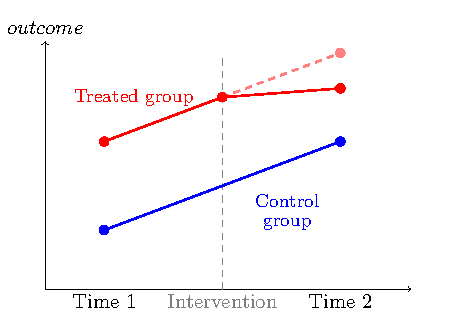
\includegraphics[width=0.5\textwidth,height=\textheight]{hei-report_files/figure-pdf/fig-didfig-1.pdf}
%DIFDELCMD < %%%
\DIFdelendFL \DIFaddbeginFL \centering{

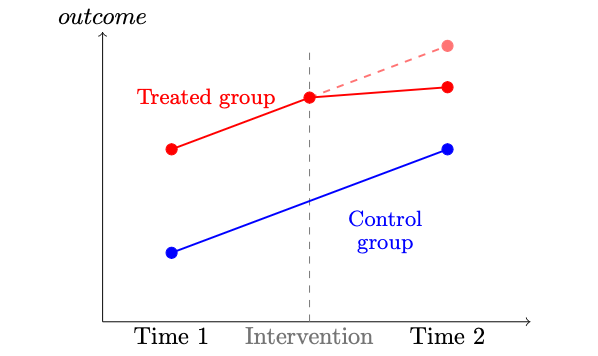
\includegraphics[width=0.75\textwidth,height=\textheight]{images/ddfig.png}

}
\DIFaddendFL 

\DIFdelbeginFL %DIFDELCMD < }
%DIFDELCMD < 

%DIFDELCMD < %%%
\DIFdelendFL \caption{\label{fig-didfig}Stylized example of
difference-in-differences}

\end{figure}%DIF > 

The DiD design compares outcomes before and after an intervention in a
treated group relative to the same outcomes measured in a control group.
The control group trend provides the crucial ``counterfactual'' estimate
of what would have happened in the treated group had it not been
treated. By comparing each group to itself, this approach helps to
control for both measured and unmeasured fixed differences between the
treated and control groups. By measuring changes over time in outcomes
in the control group unaffected by the treatment, this approach also
controls for any unmeasured factors affecting outcome trends in both
treated and control groups. This is important since there are often many
potential factors affecting outcome trends that cannot be disentangled
from the policy if one only studies the treated group (as in a
traditional pre-post design).

The canonical DiD design (Card and Krueger 1994) compares two groups
(treated and control) at two different time periods (pre- and
post-intervention, Figure~\ref{fig-didfig}). In the first time period
both groups are untreated, and in the second time period one group is
exposed to the intervention. If we assume that the differences between
the groups would have remained constant in the absence of the
intervention (the parallel trends assumption), then an unbiased estimate
of the impact of the intervention in the post-treatment period can be
calculated by subtracting the pre-post difference in the untreated group
from the pre-post difference in the treated group. The estimand of
interest in a typical DiD analysis is the average treatment effect on
the treated (i.e, the \(ATT\)), which is a contrast of the
post-intervention outcomes in the treated group with the counterfactual
estimate of outcomes in the same population in the absence of treatment.

When multiple groups are treated at different time periods, the most
common approach has been to use a two-way fixed effects model to
estimate the impact of the intervention which controls for secular
trends and differences between villages. However, recent evidence
suggests that traditional two-way fixed effects estimation of the
treatment effect may be biased in the context of heterogeneous treatment
effects, i.e., where the effects of treatment vary for different groups
treated at different time periods (Callaway and Sant'Anna 2021;
Goodman-Bacon 2021). The bias is due to the fact that the two-way fixed
effects estimate is a weighted average of several `2 x 2' DiD estimates,
some of which involve using already treated units as controls for later
treated units, which can lead to bias (Baker et al. 2022). We take
advantage of new developments in the econometrics literature (Callaway
and Sant'Anna 2021; Sun and Abraham 2021; Wooldridge 2021) that relax
the assumption of homogeneity in the context of staggered policy
rollouts but also allow straightforward interpretation of \(ATT\)s for
assessing policy impacts. This decision was motivated by the many
behavioral, social, or economic factors that might affect both new heat
pump use and coal stove suspension (e.g., energy prices and
availability, wintertime temperature, COVID-19 pandemic, user
preferences) over time in our study, and thus the possibility that the
effect of the policy on air pollution and health may be dynamic over
time and/or heterogeneous across treatment cohorts.

\DIFdelbegin %DIFDELCMD < \hypertarget{measuring-pathways-and-mechanisms}{%
%DIFDELCMD < \subsection{Measuring pathways and
%DIFDELCMD < mechanisms}\label{measuring-pathways-and-mechanisms}}
%DIFDELCMD < %%%
\DIFdelend \DIFaddbegin \subsection{\DIFadd{Measuring pathways and
mechanisms}}\label{measuring-pathways-and-mechanisms}
\DIFaddend 

To estimate how much of the CBHP intervention may work through different
mechanisms, we used causal mediation analysis. Causal approaches to
mediation attempt to discern between, and clarify the necessary
assumptions for identifying, different kinds of mediated effects. Taking
as an example the directed acyclic graph (DAG) in Figure~\ref{fig-dag1},
with \(T\) as the policy, \(X\) as a set of pre-treatment covariates,
\(M_{1}\) as PM\textsubscript{2.5}, \(M_{2}\) as indoor temperature, and
\(Y\) as systolic blood pressure, we can define the controlled direct
effect (\(CDE\)) as the effect of the CBHP policy on systolic blood
pressure if we fix the values of PM\textsubscript{2.5} and indoor
temperature to a fixed reference level for the entire population. For
example, we can estimate the impact of the policy on health outcomes
while holding PM\textsubscript{2.5} and indoor temperature at uniform
levels of average background exposure, or some other hypothetical level.

\begin{figure}[H]

\DIFdelbeginFL %DIFDELCMD < {\centering 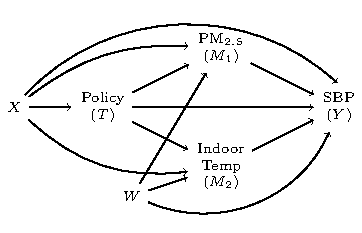
\includegraphics[width=0.6\textwidth,height=\textheight]{hei-report_files/figure-pdf/fig-dag1-1.pdf}
%DIFDELCMD < %%%
\DIFdelendFL \DIFaddbeginFL \centering{

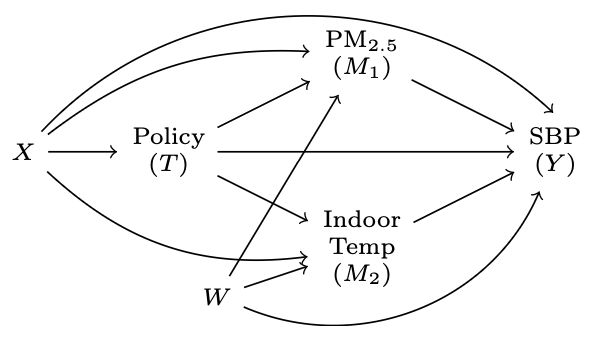
\includegraphics[width=0.6\textwidth,height=\textheight]{images/dag1.png}

}
\DIFaddendFL 

\DIFdelbeginFL %DIFDELCMD < }
%DIFDELCMD < 

%DIFDELCMD < %%%
\DIFdelendFL \caption{\label{fig-dag1}Hypothetical Directed Acyclic Graph showing
direct and indirect effects with outcome (\(Y\)), pre-treatment
covariates (\(X\)), policy (\(T\)), multiple mediators
(\(M_{1},M_{2}\)), as well as covariates for the mediators (\(W\)).}

\end{figure}%DIF > 

Although other mediated effects such as ``natural'' direct and indirect
effects are theoretically estimable (VanderWeele 2015), they involve
challenging ``cross-world'' assumptions that are difficult to anchor in
policy (Naimi et al. 2014). Other approaches to mechanisms have focused
on principal stratification (e.g., Zigler et al. 2016), although
conceptual difficulties with identifying the (unverifiable) principal
strata make it challenging for questions of mediation. Because
controlled direct effects are considered more directly policy relevant
for public health, we focused on estimating these mediated quantities.

\DIFdelbegin %DIFDELCMD < \hypertarget{data-analysis}{%
%DIFDELCMD < \section{Data Analysis}\label{data-analysis}}
%DIFDELCMD < %%%
\DIFdelend \DIFaddbegin \section{\DIFadd{Data Analysis}}\label{data-analysis}
\DIFaddend 

To understand how the policy's impact on health may be mediated by
different potential mediators, we need to first estimate the total
effect of the policy on the outcomes, then estimate the \(CDE\)s after
adjustment for potential mediators and any residual mediator-outcome
confounding. As discussed above, in order for the mediators to `explain'
the total effects of the policy on health, the policy should affect the
mediators, and the mediators should also affect the outcomes.

\DIFdelbegin %DIFDELCMD < \hypertarget{total-effect}{%
%DIFDELCMD < \subsection{Total Effect}\label{total-effect}}
%DIFDELCMD < %%%
\DIFdelend \DIFaddbegin \subsection{\DIFadd{Total Effect}}\label{total-effect}
\DIFaddend 

To estimate the total effect of the policy we used a DiD analysis that
accommodates staggered treatment rollout. To allow for heterogeneity in
the context of staggered rollout we used `extended' two-way fixed
effects (ETWFE) models (Wooldridge 2021) to estimate the total effect of
the CBHP policy. The mean outcome (replaced by a suitable link function
\(g(\cdot)\) for binary or count outcomes) was defined using a set of
linear predictors:

\begin{equation}\DIFdelbegin %DIFDELCMD < \protect\hypertarget{eq-etwfe}{}{Y_{ijt}=g(\mu_{ijt}) = \alpha + \sum_{r=q}^{T} \beta_{r} d_{r} + \sum_{s=r}^{T} \gamma_{s} fs_{t}+ \sum_{r=q}^{T} \sum_{s=r}^{T} \tau_{rt} (d_{r} \times fs_{t}) + \varepsilon_{ijt}}\label{eq-etwfe}%%%
\DIFdelend \DIFaddbegin \phantomsection\label{eq-etwfe}{Y_{ijt}=g(\mu_{ijt}) = \alpha + \sum_{r=q}^{T} \beta_{r} d_{r} + \sum_{s=r}^{T} \gamma_{s} fs_{t}+ \sum_{r=q}^{T} \sum_{s=r}^{T} \tau_{rt} (d_{r} \times fs_{t}) + \varepsilon_{ijt}}\DIFaddend \end{equation}

where \(Y_{ijt}\) is the outcome for individual \(i\) in village \(j\)
at time \(t\), \(d_{r}\) represent treatment cohort dummies, i.e., fixed
effects for cohorts of villages that were first exposed to the policy at
the same time \(q\) (e.g., in 2019, 2020, or 2021), \(fs_{t}\) are time
fixed effects corresponding to different winter data collection waves
(2018-19, 2019-20, or 2021-22), and \(\tau_{rt}\) are the cohort-time
\(ATT\)s in the context of a linear model. For binary or count outcomes
the cohort-time \(ATT\)s are derived by estimating marginal effects from
non-linear models (Arel-Bundock 2024). For all models we cluster
standard errors at the village level, consistent with the unit of
treatment assignment (Cameron and Miller 2015). The ETWFE and other
approaches that allow for several (potentially heterogeneous) treatment
effects may also be averaged to provide a weighted summary \(ATT\).
Several potential possibilities are feasible, including weighting by
treatment cohorts or time since policy adoption (Goin and Riddell 2023).
We generally focus on two types of \(ATT\)s for this report: simple
averages across all treatment cohorts and the full set of cohort-time
\(ATT\)s to evaluate heterogeneous treatment effects. Although we
primarily focus on reporting the simple average \(ATT\) for most
outcomes, we also used omnibus joint \emph{F}-tests to assess whether
there was sufficient evidence to reject the assumption of homogeneity
across the \(ATT\)s.

\DIFdelbegin %DIFDELCMD < \hypertarget{mediation-analysis}{%
%DIFDELCMD < \subsection{Mediation Analysis}\label{mediation-analysis}}
%DIFDELCMD < %%%
\DIFdelend \DIFaddbegin \subsection{\DIFadd{Mediation Analysis}}\label{mediation-analysis}
\DIFaddend 

As noted above, with respect to the mediation analysis we are chiefly
interested in the \(CDE\), which can be derived by adding relevant
mediators \(M\) to Equation~\ref{eq-etwfe}. If we also allow for
exposure-mediator interaction and potentially allow for adjustment for
confounders \(W\) of the mediator-outcome effect, we can extend equation
Equation~\ref{eq-etwfe} as follows:

\begin{equation}\DIFdelbegin %DIFDELCMD < \protect\hypertarget{eq-etwfem}{}{
%DIFDELCMD < \begin{aligned}
%DIFDELCMD < Y_{ijt}=g(\mu_{ijt}) = \alpha + \sum_{r=q}^{T} \beta_{r} d_{r} + \sum_{s=r}^{T} \gamma_{s} fs_{t}+ \sum_{r=q}^{T} \sum_{s=r}^{T} \tau_{rt} (d_{r} \times fs_{t}) \\ + \delta M_{it} + \sum_{r=q}^{T} \sum_{s=r}^{T} \eta_{rt} (d_{r} \times fs_{t} \times M_{it}) + \zeta \mathbf{W} + \varepsilon_{ijt}
%DIFDELCMD < \end{aligned}
%DIFDELCMD < }\label{eq-etwfem}%%%
\DIFdelend \DIFaddbegin \phantomsection\label{eq-etwfem}{
\begin{aligned}
Y_{ijt}=g(\mu_{ijt}) = \alpha + \sum_{r=q}^{T} \beta_{r} d_{r} + \sum_{s=r}^{T} \gamma_{s} fs_{t}+ \sum_{r=q}^{T} \sum_{s=r}^{T} \tau_{rt} (d_{r} \times fs_{t}) \\ + \delta M_{it} + \sum_{r=q}^{T} \sum_{s=r}^{T} \eta_{rt} (d_{r} \times fs_{t} \times M_{it}) + \zeta \mathbf{W} + \varepsilon_{ijt}
\end{aligned}
}\DIFaddend \end{equation}

where now \(\delta\) is the conditional effect of the mediator \(M\) at
the reference level of the treatment (again, represented via the series
of group-time interaction terms), and the collection of \(\eta\) terms
are coefficients for the product terms allowing for mediator-treatment
interaction. Finally, \(\zeta\) is a vector of coefficients for the set
of confounders contained within \(\mathbf{W}\).

As noted above, in the staggered DiD framework that allows for
heterogeneity we do not have a single treatment effect but a collection
of group-time treatment effects that may be averaged in different ways.
This extends to the estimation of the \(CDE\), in which case we will
also have several \(CDE\)s that can be averaged to make inferences about
the extent to which the policy's impact is mediated by
PM\textsubscript{2.5}. Based on the setup in Equation~\ref{eq-etwfem}
the \(CDE\) is estimated as: \(\delta + \eta_{rt}MT\). In the absence of
interaction between the exposure and the mediator (i.e.,
\(\eta_{rt}=0\)) the \(CDE\) will simply be the estimated treatment
effects \(\sum_{r=q}^{T} \sum_{s=r}^{T} \tau_{rt}\), i.e., the effect of
the policy holding \(M\) constant. For a valid estimate of the \(CDE\)
we must account for confounding of the mediator-outcome effect,
represented by \(W\) in the equation above. The inclusion of baseline
measures of both the outcome and the proposed mediators inherent in our
DiD strategy help to reduce the potential for unmeasured confounding of
the mediator-outcome effect (Keele et al. 2015). Given the large number
of outcomes of interest in this study, as well as the potential for
heterogeneous treatment effects, we limited the mediation analysis to
health outcomes for which we observed a total effect of the CBHP policy.

\DIFdelbegin %DIFDELCMD < \hypertarget{identification-of-potential-confounders-and-model-covariates}{%
%DIFDELCMD < \subsection{Identification of potential confounders and model
%DIFDELCMD < covariates}\label{identification-of-potential-confounders-and-model-covariates}}
%DIFDELCMD < %%%
\DIFdelend \DIFaddbegin \subsection{\DIFadd{Identification of potential confounders and model
covariates}}\label{identification-of-potential-confounders-and-model-covariates}
\DIFaddend 

In contrast to typical analytic approaches such as regression adjustment
or propensity scores that solely focus on measured covariates, our DiD
approach helps to minimize the risk of some sources of \emph{unmeasured}
confounding. Treatment cohort fixed effects control for measured and
unmeasured time-constant factors that may differ between treatment
cohorts (e.g., genetics, altitude), and time fixed effects control for
secular trends, capturing any unmeasured factors that affect outcomes in
all treatment cohorts (including the untreated) similarly over the study
period (e.g., background improvements in ambient air quality or
household transition to more efficient heating). The latter are
particularly helpful in the context of the documented declines in
PM\textsubscript{2.5} in China attributable to sources other than the
CBHP policy (Van Donkelaar et al. 2021; Zhang et al. 2019)

For models estimating the effect of the policy on health outcomes, we
used DAGs (Pearl 2000) to identify potential time-varying causes of both
treatment by the policy and our study outcome(s) that could differ
between treatment groups, and adjusted for those potential confounders
in the regression models. For the mediation analysis, we identified
potential mediator-outcome confounders using the same approach. These
variables were identified from the relevant peer-reviewed literature and
our team's substantive knowledge about the CBHP policy. In the
multivariable models, we also adjusted for strong predictors of the
outcome that were not affected by treatment, and thus not confounders,
to improve model precision. The covariates included in each of the
models are provided in the tables.

For air pollution outcomes, we considered the following covariates:
village population and total number of households in the village;
temperature, relative humidity, wind direction, wind speed, boundary
layer height; home area and home area heated; home insulation; smoking
status of participant and whether or not they lived with a smoker;
whether or not the household reported using wood (i.e., biomass) for
household energy activities, and if so, self-reported quantity of wood.
Potential non-linearity between continuous covariates and our study
outcomes were evaluated using natural cubic splines with different
degrees of freedom. Ultimately, the following covariates were included
in the final DiD models for outdoor, indoor, and personal exposures to
air pollution, based on whether measurable changes in the covariate over
time were observed. For the final adjusted DiD model for personal
exposure source contributions due to mixed combustion of solid fuels
(hereafter `mixed combustion'), we adjusted for: temperature
(represented by a spline with 2 degrees of freedom); participant smoking
status; and whether or not the household reported using biomass fuel.
For the final adjusted DiD model for outdoor (community) `mixed
combustion' source contributions, the following covariates were
included: total number of households in the village; village population;
and ambient relative humidity (represented by a spline with 2 degrees of
freedom).

\DIFdelbegin %DIFDELCMD < \hypertarget{multiple-imputation-for-covariates-and-indoor-pm2.5-in-analyses-with-bp-outcomes}{%
%DIFDELCMD < \subsection{\texorpdfstring{Multiple imputation for covariates and
%DIFDELCMD < indoor PM\textsubscript{2.5} in analyses with BP
%DIFDELCMD < outcomes}{Multiple imputation for covariates and indoor PM2.5 in analyses with BP outcomes}}\label{multiple-imputation-for-covariates-and-indoor-pm2.5-in-analyses-with-bp-outcomes}}
%DIFDELCMD < %%%
\DIFdelend \DIFaddbegin \subsection{\texorpdfstring{Multiple imputation for covariates and
indoor PM\textsubscript{2.5} in analyses with BP
outcomes}{Multiple imputation for covariates and indoor PM2.5 in analyses with BP outcomes}}\label{multiple-imputation-for-covariates-and-indoor-pm2.5-in-analyses-with-bp-outcomes}
\DIFaddend 

Blood pressure was measured at household visits but several key
covariates like waist circumference, height, and weight were measured at
the clinic visits in w1 and w2. Thus, we were missing covariate
information for individuals who were unable to attend the clinic visits
(\textasciitilde15-20\% of participants in each wave). Additionally,
since we only measured indoor PM\textsubscript{2.5} in a subsample of
300 homes in w2 and w4, we were missing indoor PM\textsubscript{2.5} for
all participants in w1 with BP measures, as well as for a sub-sample of
participants in w2 and w4. To prepare data for the BP outcomes analysis
we used multiple imputation with chained equations (MICE) to impute
missing covariate data and missing indoor PM\textsubscript{2.5} values
for individuals who participated in the household visit but not the
clinic visit. This allowed us to retain observations with BP
measurements that would have otherwise been dropped in adjusted and
mediation models using complete-case analysis. Imputation was performed
with the \emph{MICE} package (van Buuren and Groothuis-Oudshoorn 2011)
in \emph{R} (m = 30 imputation datasets, with 30 iterations each), and
the difference-in-differences and mediation analyses were conducted for
each of the 30 datasets. We then used Rubin's Rules to combine point
estimates and standard errors while accounting for both within- and
between-dataset variances (Rubin 1987). In Appendix
Figure~\ref{fig-afig-mi} we show kernel density plots for the
distribution of imputed values for BMI, waist circumference, and indoor
PM\textsubscript{2.5}, all of which closely approximated the observed
values.

\DIFdelbegin %DIFDELCMD < \hypertarget{results-1}{%
%DIFDELCMD < \section{Results}\label{results-1}}
%DIFDELCMD < %%%
\DIFdelend \DIFaddbegin \section{\DIFadd{Results}}\label{results-1}
\DIFaddend 

We retained all 50 study villages during this four-year longitudinal
assessment of village treatment by the CBHP policy, though we were only
able to visit 41 villages in winter 2020-21 (w3) and were limited to
village and household-level measurements of air quality, indoor
temperature, and stove use in that wave due to restrictions during the
COVID pandemic.

By w2, w3, and w4 there were a cumulative total of 10, 17, and 20 (out
of 50 total) study villages treated by the CBHP policy, respectively.
All of the treated villages selected to install electric-powered
air-source heat pumps with 200 RMB per meter square (up to 24,000 RMB)
in subsidies and were also provided with 80\% night-time electricity
subsidies up to 10,000kWh per heating season. To limit coal use,
villages enrolled in the policy were no longer allowed to place orders
for subsidized coal with the district-level governments that manage the
procurement and distribution of coal for residential heating in Beijing.
In addition, village committee leaders in treated villages reported
feeling accountable to the Environmental Protection Department for
limited coal-related air pollution, and were motivated to encourage
residents to not burn coal. Some villages were equipped with government
air pollution monitors and the Environmental Protection Department
conducted village inspections and issued warnings about coal burning.
Households burning coal in treated villages were at risk of losing their
electricity subsidy.

Appendix Figure~\ref{fig-flowchart} shows the participation of villages,
households, and participants across the four waves of data collection.
We conducted measurements in over 1000 participants in each of the three
measurement waves that included individual-level measurements. In total,
we enrolled 1432 participants into the study, of which 630 (43\%)
\DIFdelbegin \DIFdel{participated in }\DIFdelend \DIFaddbegin \DIFadd{individual contributed 1890 observations across }\DIFaddend all three waves, 443
(31\%) \DIFdelbegin \DIFdel{participated in }\DIFdelend \DIFaddbegin \DIFadd{individuals contributed 886 observations across }\DIFaddend two waves and 365
(25\%) \DIFaddbegin \DIFadd{individuals }\DIFaddend participated in a single wave. \DIFdelbegin \DIFdel{We did not observe any
notable differences in demographic characteristics or }\DIFdelend \DIFaddbegin \DIFadd{Table 3 shows selected
demographic characteristics and }\DIFaddend health behaviors between participants
who contributed to \DIFdelbegin \DIFdel{a different number of waves(Table ~\ref{tbl-each-campaign}) }\DIFdelend \DIFaddbegin \DIFadd{each study wave. We find no differences in gender or
smoking across waves, but overall BMI and waist circumference increased
over time. Table 4 shows similar measures according to whether }\DIFaddend or
between participants in each of the three waves with individual
measurements (\DIFdelbegin \DIFdel{Table~\ref{tbl-diff-campaign}}\DIFdelend \DIFaddbegin \textbf{\DIFadd{?@tbl-diff-campaign}}\DIFaddend ).

\DIFdelbegin %DIFDELCMD < \hypertarget{tbl-each-campaign}{}
%DIFDELCMD < \begin{table}
%DIFDELCMD < %%%
%DIFDELCMD < \caption{%
{%DIFAUXCMD
%DIFDELCMD < \label{tbl-each-campaign}%%%
\DIFdelFL{Demographic and health characteristics of participants in each study
wave }}%DIFAUXCMD
%DIFDELCMD < \tabularnewline
%DIFDELCMD < %%%
\DIFdelendFL \DIFaddbeginFL \subsection{\DIFaddFL{Description of study
sample}}\label{description-of-study-sample}
\DIFaddendFL 

\DIFdelbeginFL %DIFDELCMD < \centering
%DIFDELCMD < \begin{tabular}{l>{\centering\arraybackslash}p{2.5cm}>{\centering\arraybackslash}p{2.5cm}>{\centering\arraybackslash}p{2.5cm}}
%DIFDELCMD < \toprule
%DIFDELCMD < %%%
\textbf{\DIFdelFL{Characteristic}} %DIFAUXCMD
%DIFDELCMD < & %%%
\textbf{\DIFdelFL{Wave 1 (2018-19) N=1003}} %DIFAUXCMD
%DIFDELCMD < & %%%
\textbf{\DIFdelFL{Wave 2 (2019-20) N=1110}} %DIFAUXCMD
%DIFDELCMD < & %%%
\textbf{\DIFdelFL{Wave 4 (2021-22) N=1028}}%DIFAUXCMD
%DIFDELCMD < \\
%DIFDELCMD < \midrule
%DIFDELCMD < %%%
\DIFdelFL{Female, n (\%) }%DIFDELCMD < & %%%
\DIFdelFL{580 (57.8) }%DIFDELCMD < & %%%
\DIFdelFL{653 (58.8) }%DIFDELCMD < & %%%
\DIFdelFL{612 (59.5)}%DIFDELCMD < \\
%DIFDELCMD < %%%
\DIFdelFL{Current smoker, n (\%) }%DIFDELCMD < & %%%
\DIFdelFL{257 (25.6) }%DIFDELCMD < & %%%
\DIFdelFL{295 (26.6) }%DIFDELCMD < & %%%
\DIFdelFL{265 (25.8)}%DIFDELCMD < \\
%DIFDELCMD < %%%
\DIFdelFL{Any smoke exposure, n (\%) }%DIFDELCMD < & %%%
\DIFdelFL{788 (78.6) }%DIFDELCMD < & %%%
\DIFdelFL{897 (80.8) }%DIFDELCMD < & %%%
\DIFdelFL{843 (82)}%DIFDELCMD < \\
%DIFDELCMD < %%%
\DIFdelFL{Age in years, Mean (SD) }%DIFDELCMD < & %%%
\DIFdelFL{60.7 (9.2) }%DIFDELCMD < & %%%
\DIFdelFL{61.4 (9.1) }%DIFDELCMD < & %%%
\DIFdelFL{63.1 (9)}%DIFDELCMD < \\
%DIFDELCMD < %%%
\DIFdelFL{BMI in kg/m\textsuperscript{2}, Mean (SD) }%DIFDELCMD < & %%%
\DIFdelFL{26.1 (3.7) }%DIFDELCMD < & %%%
\DIFdelFL{25.7 (3.5) }%DIFDELCMD < & %%%
\DIFdelFL{26.1 (4)}%DIFDELCMD < \\
%DIFDELCMD < %%%
\DIFdelFL{Waist circumference in cm, Mean (SD) }%DIFDELCMD < & %%%
\DIFdelFL{86.8 (10.2) }%DIFDELCMD < & %%%
\DIFdelFL{87.4 (9.4) }%DIFDELCMD < & %%%
\DIFdelFL{91.4 (10.7)}%DIFDELCMD < \\
%DIFDELCMD < \bottomrule
%DIFDELCMD < \end{tabular}
%DIFDELCMD < \end{table}
%DIFDELCMD < 

%DIFDELCMD < \hypertarget{tbl-diff-campaign}{}
%DIFDELCMD < %%%
\DIFdelend \begin{table}
\DIFdelbeginFL %DIFDELCMD < \caption{%
{%DIFAUXCMD
%DIFDELCMD < \label{tbl-diff-campaign}%%%
\DIFdelFL{Demographic and health characteristics of participants who contributed
to different numbers of study waves. }}%DIFAUXCMD
%DIFDELCMD < \tabularnewline
%DIFDELCMD < 

%DIFDELCMD < %%%
\DIFdelendFL \centering\DIFdelbeginFL %DIFDELCMD < \begin{tabular}{l>{\centering\arraybackslash}p{2.5cm}>{\centering\arraybackslash}p{2.5cm}>{\centering\arraybackslash}p{2.5cm}}
%DIFDELCMD < \toprule
%DIFDELCMD < %%%
\textbf{\DIFdelFL{Characteristic}} %DIFAUXCMD
%DIFDELCMD < & %%%
\textbf{\DIFdelFL{1 Wave N=365}} %DIFAUXCMD
%DIFDELCMD < & %%%
\textbf{\DIFdelFL{2 Waves N=443}} %DIFAUXCMD
%DIFDELCMD < & %%%
\textbf{\DIFdelFL{3 Waves N=630}}%DIFAUXCMD
%DIFDELCMD < \\
%DIFDELCMD < \midrule
%DIFDELCMD < %%%
\DIFdelFL{Female, n (\%) }%DIFDELCMD < & %%%
\DIFdelFL{211 (57.8) }%DIFDELCMD < & %%%
\DIFdelFL{253 (57.1) }%DIFDELCMD < & %%%
\DIFdelFL{370 (58.7)}%DIFDELCMD < \\
%DIFDELCMD < %%%
\DIFdelFL{Current smoker, n (\%) }%DIFDELCMD < & %%%
\DIFdelFL{110 (30.1) }%DIFDELCMD < & %%%
\DIFdelFL{117 (26.4) }%DIFDELCMD < & %%%
\DIFdelFL{161 (25.6)}%DIFDELCMD < \\
%DIFDELCMD < %%%
\DIFdelFL{Any smoke exposure, n (\%) }%DIFDELCMD < & %%%
\DIFdelFL{288 (78.9) }%DIFDELCMD < & %%%
\DIFdelFL{360 (81.3) }%DIFDELCMD < & %%%
\DIFdelFL{498 (79)}%DIFDELCMD < \\
%DIFDELCMD < %%%
\DIFdelFL{Age in years, Mean (SD) }%DIFDELCMD < & %%%
\DIFdelFL{59.9 (9.2) }%DIFDELCMD < & %%%
\DIFdelFL{60.5 (8.8) }%DIFDELCMD < & %%%
\DIFdelFL{61.3 (9.1)}%DIFDELCMD < \\
%DIFDELCMD < %%%
\DIFdelFL{BMI in kg/m\textsuperscript{2}, Mean (SD) }%DIFDELCMD < & %%%
\DIFdelFL{26.3 (3.6) }%DIFDELCMD < & %%%
\DIFdelFL{25.8 (3.5) }%DIFDELCMD < & %%%
\DIFdelFL{26.1 (3.7)}%DIFDELCMD < \\
%DIFDELCMD < %%%
\DIFdelFL{Waist circumference in cm, Mean (SD) }%DIFDELCMD < & %%%
\DIFdelFL{90.3 (9.8) }%DIFDELCMD < & %%%
\DIFdelFL{86.5 (10) }%DIFDELCMD < & %%%
\DIFdelFL{86.9 (10.4)}%DIFDELCMD < \\
%DIFDELCMD < \bottomrule
%DIFDELCMD < \end{tabular}
%DIFDELCMD < \end{table}
%DIFDELCMD < 

%DIFDELCMD < \hypertarget{description-of-study-sample}{%
%DIFDELCMD < \subsection{Description of study
%DIFDELCMD < sample}\label{description-of-study-sample}}
%DIFDELCMD < 

%DIFDELCMD < \hypertarget{tbl-table1}{}
%DIFDELCMD < \begin{table}
%DIFDELCMD < %%%
%DIFDELCMD < \caption{%
{%DIFAUXCMD
%DIFDELCMD < \label{tbl-table1}%%%
\DIFdelFL{Descriptive statistics for selected demographic, health, and
environmental measures at baseline, by treatment status }}%DIFAUXCMD
%DIFDELCMD < \tabularnewline
%DIFDELCMD < 

%DIFDELCMD < %%%
\DIFdelendFL \centering
\DIFaddbeginFL \caption{\label{tab:table1}\DIFaddFL{Descriptive statistics for selected demographic, health, and environmental measures at baseline, by treatment status.}}
\DIFaddendFL \centering
\fontsize{9}{11}\selectfont
\begin{tabular}[t]{rrrrrrr}
\toprule
\multicolumn{1}{c}{ } & \multicolumn{2}{c}{Never treated (N=603)} & \multicolumn{2}{c}{Ever treated (N=400)} & \multicolumn{2}{c}{ } \\
\cmidrule(l{3pt}r{3pt}){2-3} \cmidrule(l{3pt}r{3pt}){4-5}
  & Mean & Std. Dev. & Mean & Std. Dev. & Diff. in Means & Std. Error\\
\midrule
\textbf{Demographics:} & \textbf{} & \textbf{} & \textbf{} & \textbf{} & \textbf{} & \textbf{}\\
Age (years) & 59.9 & 9.4 & 60.4 & 9.2 & 0.5 & 0.6\\
Female (\%) & 59.5 & 49.1 & 59.1 & 49.2 & -0.4 & 3.2\\
No education (\%) & 11.5 & 31.9 & 12.3 & 32.9 & 0.9 & 2.1\\
Primary education (\%) & 75.5 & 43.0 & 77.6 & 41.7 & 2.1 & 2.8\\
Secondary+ education (\%) & 12.6 & 33.2 & 9.8 & 29.7 & -2.9 & 2.0\\
\textbf{Health measures:} & \textbf{} & \textbf{} & \textbf{} & \textbf{} & \textbf{} & \textbf{}\\
Never smoker (\%) & 61.9 & 48.6 & 59.5 & 49.1 & -2.4 & 3.2\\
Former smoker (\%) & 11.9 & 32.4 & 15.1 & 35.8 & 3.2 & 2.2\\
Current smoker (\%) & 26.2 & 44.0 & 25.4 & 43.6 & -0.8 & 2.8\\
Never drinker (\%) & 55.9 & 49.7 & 52.5 & 50.0 & -3.4 & 3.2\\
Occasional drinker (\%) & 26.0 & 43.9 & 25.5 & 43.6 & -0.5 & 2.8\\
Daily drinker (\%) & 17.8 & 38.3 & 21.9 & 41.4 & 4.1 & 2.6\\
Systolic (mmHg) & 131.4 & 16.8 & 128.7 & 14.3 & -2.7 & 1.0\\
Diastolic (mmHg) & 82.7 & 11.6 & 82.1 & 11.3 & -0.6 & 0.8\\
Waist circumference (cm) & 87.7 & 10.5 & 85.4 & 9.5 & -2.3 & 0.8\\
Body mass index (kg/m2) & 26.3 & 3.7 & 25.8 & 3.6 & -0.5 & 0.3\\
Frequency of coughing (\%) & 18.7 & 39.0 & 19.7 & 39.8 & 1.0 & 2.6\\
Frequency of wheezing (\%) & 6.2 & 24.2 & 6.6 & 24.8 & 0.3 & 1.6\\
Shortness of breath (\%) & 29.2 & 45.5 & 34.3 & 47.5 & 5.1 & 3.0\\
Chest trouble (\%) & 11.6 & 32.0 & 14.1 & 34.9 & 2.5 & 2.2\\
Any respiratory problem (\%) & 50.6 & 50.0 & 54.3 & 49.9 & 3.7 & 3.2\\
\textbf{Environmental measures:} & \textbf{} & \textbf{} & \textbf{} & \textbf{} & \textbf{} & \textbf{}\\
Temperature (°C) & 13.8 & 3.6 & 13.5 & 3.3 & -0.3 & 0.2\\
Personal PM2.5 (ug/m3) & 150.2 & 300.3 & 103.8 & 107.3 & -46.3 & 19.1\\
\bottomrule
\end{tabular}
\end{table}

Table \DIFdelbegin \DIFdel{~\ref{tbl-table1} }\DIFdelend \DIFaddbegin \DIFadd{4 }\DIFaddend shows the distribution of selected demographic, health, and
environmental characteristics from the baseline survey, prior to any
villages being enrolled in the CBHP policy. We provide means and
standard deviations separately for villages that eventually enter into
the policy with those that never do so. As noted above, although our DiD
identification strategy allows for fixed differences between treated and
untreated villages, overall the differences at baseline are generally
small and the groups seem well balanced on most measures, with the
exception of personal exposure to PM\textsubscript{2.5}, which was lower
in villages that were eventually treated.

\DIFdelbegin %DIFDELCMD < \hypertarget{summary-of-pm-and-bc-measurements}{%
%DIFDELCMD < \subsection{Summary of PM and BC
%DIFDELCMD < measurements}\label{summary-of-pm-and-bc-measurements}}
%DIFDELCMD < %%%
\DIFdelend \DIFaddbegin \subsection{\DIFadd{Summary of PM and BC
measurements}}\label{summary-of-pm-and-bc-measurements}
\DIFaddend 

At baseline, PM\textsubscript{2.5} and BC concentrations were higher, on
average, for personal exposures compared with outdoor concentrations.
From w2 onward, with the inclusion of indoor air pollution measurements,
personal exposure air pollution concentrations were still higher than
indoor or outdoor concentrations, with indoor levels being higher than
outdoors (Table~\ref{tbl-pm-season}). This trend (personal
\textgreater{} indoor \textgreater{} outdoor) was observed among
households in treated and untreated villages. Personal, indoor, and
outdoor geometric mean (95\% confidence interval) concentrations of
PM\textsubscript{2.5} were 72 (65, 80), 45 (39, 53), and 31 (28, 35),
respectively, and elevated relative to health-based guidelines. The
current World Health Organization (WHO) guidelines state that annual
average concentrations of PM\textsubscript{2.5} should not exceed 5
µg/m\textsuperscript{3}, while 24-hour average exposures should not
exceed 15 µg/m\textsuperscript{3} for more than 3 to 4 days per year
(World Health Organization 2021). Interim targets have been set to
support the planning of incremental milestones toward cleaner air,
particularly for cities, regions, and countries with higher air
pollution levels. For PM\textsubscript{2.5}, the four interim (IT)
targets for annual and 24-h means are: IT-1: 35 and 75
µg/m\textsuperscript{3}; IT-2: 25 and 50 µg/m\textsuperscript{3}; IT-3:
15 and 37.5 µg/m\textsuperscript{3}; and IT-4: 10 and 25
µg/m\textsuperscript{3} (World Health Organization 2021). In our study,
baseline personal exposures to PM\textsubscript{2.5} did not even meet
IT-1, indicating considerable opportunity for air quality exposure
reduction with intervention.

\DIFdelbegin %DIFDELCMD < \hypertarget{tbl-pm-season}{}
%DIFDELCMD < %%%
\DIFdelend \begin{table}
\DIFdelbeginFL %DIFDELCMD < \caption{%
{%DIFAUXCMD
%DIFDELCMD < \label{tbl-pm-season}%%%
\DIFdelFL{Arithmetic and geometric means for air pollutant concentrations
(micrograms per cubic meter) by wave }}%DIFAUXCMD
%DIFDELCMD < \tabularnewline
%DIFDELCMD < %%%
\DIFdelendFL 

\DIFdelbeginFL %DIFDELCMD < \centering\begingroup\fontsize{9}{11}\selectfont
%DIFDELCMD < %%%
\DIFdelendFL \DIFaddbeginFL \caption{\label{tbl-pm-season}\DIFaddFL{Arithmetic and geometric means for air
pollutant concentrations (micrograms per cubic meter) by wave}}
\DIFaddendFL 

\DIFdelbeginFL %DIFDELCMD < \begin{tabular}{lllcccccccc}
%DIFDELCMD < \toprule
%DIFDELCMD < \multicolumn{3}{c}{ } & \multicolumn{2}{c}{Wave 1} & \multicolumn{2}{c}{Wave 2} & \multicolumn{2}{c}{Wave 3} & \multicolumn{2}{c}{Wave 4} \\
%DIFDELCMD < \cmidrule%%%
\DIFdelFL{(l}%DIFDELCMD < {%%%
\DIFdelFL{3pt}%DIFDELCMD < }%%%
\DIFdelFL{r}%DIFDELCMD < {%%%
\DIFdelFL{3pt}%DIFDELCMD < }%%%
\DIFdelFL{)}%DIFDELCMD < {%%%
\DIFdelFL{4-5}%DIFDELCMD < } \cmidrule%%%
\DIFdelFL{(l}%DIFDELCMD < {%%%
\DIFdelFL{3pt}%DIFDELCMD < }%%%
\DIFdelFL{r}%DIFDELCMD < {%%%
\DIFdelFL{3pt}%DIFDELCMD < }%%%
\DIFdelFL{)}%DIFDELCMD < {%%%
\DIFdelFL{6-7}%DIFDELCMD < } \cmidrule%%%
\DIFdelFL{(l}%DIFDELCMD < {%%%
\DIFdelFL{3pt}%DIFDELCMD < }%%%
\DIFdelFL{r}%DIFDELCMD < {%%%
\DIFdelFL{3pt}%DIFDELCMD < }%%%
\DIFdelFL{)}%DIFDELCMD < {%%%
\DIFdelFL{8-9}%DIFDELCMD < } \cmidrule%%%
\DIFdelFL{(l}%DIFDELCMD < {%%%
\DIFdelFL{3pt}%DIFDELCMD < }%%%
\DIFdelFL{r}%DIFDELCMD < {%%%
\DIFdelFL{3pt}%DIFDELCMD < }%%%
\DIFdelFL{)}%DIFDELCMD < {%%%
\DIFdelFL{10-11}%DIFDELCMD < }
%DIFDELCMD <  &  &  & %%%
\DIFdelFL{Est. }%DIFDELCMD < & %%%
\DIFdelFL{CI }%DIFDELCMD < & %%%
\DIFdelFL{Est. }%DIFDELCMD < & %%%
\DIFdelFL{CI }%DIFDELCMD < & %%%
\DIFdelFL{Est. }%DIFDELCMD < & %%%
\DIFdelFL{CI }%DIFDELCMD < & %%%
\DIFdelFL{Est. }%DIFDELCMD < & %%%
\DIFdelFL{CI}%DIFDELCMD < \\
%DIFDELCMD < \midrule
%DIFDELCMD < \addlinespace[0.3em]
%DIFDELCMD < \multicolumn{11}{l}{\textbf{Personal}}\\
%DIFDELCMD <  &  & %%%
\DIFdelFL{Mean }%DIFDELCMD < & %%%
\DIFdelFL{117 }%DIFDELCMD < & {}[%%%
\DIFdelFL{105, 129}%DIFDELCMD < ] & %%%
\DIFdelFL{97 }%DIFDELCMD < & {}[%%%
\DIFdelFL{87, 107}%DIFDELCMD < ] &  &  & %%%
\DIFdelFL{84 }%DIFDELCMD < & {}[%%%
\DIFdelFL{72, 97}%DIFDELCMD < ]\\
%DIFDELCMD < \cmidrule{3-11}
%DIFDELCMD <  & \multirow[t]{-2}{*}{\raggedright\arraybackslash 24h PM2.5} & %%%
\DIFdelFL{GM }%DIFDELCMD < & %%%
\DIFdelFL{72 }%DIFDELCMD < & {}[%%%
\DIFdelFL{65, 80}%DIFDELCMD < ] & %%%
\DIFdelFL{59 }%DIFDELCMD < & {}[%%%
\DIFdelFL{53, 65}%DIFDELCMD < ] &  &  & %%%
\DIFdelFL{47 }%DIFDELCMD < & {}[%%%
\DIFdelFL{42, 52}%DIFDELCMD < ]\\
%DIFDELCMD < \cmidrule{2-11}
%DIFDELCMD <  &  & %%%
\DIFdelFL{Mean }%DIFDELCMD < & %%%
\DIFdelFL{4 }%DIFDELCMD < & {}[%%%
\DIFdelFL{3.5, 4.4}%DIFDELCMD < ] & %%%
\DIFdelFL{3.5 }%DIFDELCMD < & {}[%%%
\DIFdelFL{2.7, 4.2}%DIFDELCMD < ] &  &  & %%%
\DIFdelFL{3.7 }%DIFDELCMD < & {}[%%%
\DIFdelFL{2.9, 4.5}%DIFDELCMD < ]\\
%DIFDELCMD < \cmidrule{3-11}
%DIFDELCMD < \multirow[t]{-4}{*}[1\dimexpr\aboverulesep+\belowrulesep+\cmidrulewidth]{\raggedright\arraybackslash Filter-derived} & \multirow[t]{-2}{*}{\raggedright\arraybackslash 24h BC} & %%%
\DIFdelFL{GM }%DIFDELCMD < & %%%
\DIFdelFL{2.6 }%DIFDELCMD < & {}[%%%
\DIFdelFL{2.4, 2.8}%DIFDELCMD < ] & %%%
\DIFdelFL{1.9 }%DIFDELCMD < & {}[%%%
\DIFdelFL{1.7, 2.1}%DIFDELCMD < ] &  &  & %%%
\DIFdelFL{1.7 }%DIFDELCMD < & {}[%%%
\DIFdelFL{1.5, 1.9}%DIFDELCMD < ]\\
%DIFDELCMD < \cmidrule{1-11}
%DIFDELCMD < \addlinespace[0.3em]
%DIFDELCMD < \multicolumn{11}{l}{\textbf{Indoor}}\\
%DIFDELCMD <  &  & %%%
\DIFdelFL{Mean }%DIFDELCMD < &  &  & %%%
\DIFdelFL{94 }%DIFDELCMD < & {}[%%%
\DIFdelFL{84, 104}%DIFDELCMD < ] & %%%
\DIFdelFL{84 }%DIFDELCMD < & {}[%%%
\DIFdelFL{75, 94}%DIFDELCMD < ] & %%%
\DIFdelFL{67 }%DIFDELCMD < & {}[%%%
\DIFdelFL{60, 75}%DIFDELCMD < ]\\
%DIFDELCMD < \cmidrule{3-11}
%DIFDELCMD < \multirow[t]{-2}{*}{\raggedright\arraybackslash Sensor-derived} & \multirow[t]{-2}{*}{\raggedright\arraybackslash Seasonal PM2.5} & %%%
\DIFdelFL{GM }%DIFDELCMD < &  &  & %%%
\DIFdelFL{71 }%DIFDELCMD < & {}[%%%
\DIFdelFL{65, 78}%DIFDELCMD < ] & %%%
\DIFdelFL{63 }%DIFDELCMD < & {}[%%%
\DIFdelFL{57, 70}%DIFDELCMD < ] & %%%
\DIFdelFL{47 }%DIFDELCMD < & {}[%%%
\DIFdelFL{42, 52}%DIFDELCMD < ]\\
%DIFDELCMD < \cmidrule{1-11}
%DIFDELCMD <  &  & %%%
\DIFdelFL{Mean }%DIFDELCMD < &  &  & %%%
\DIFdelFL{69 }%DIFDELCMD < & {}[%%%
\DIFdelFL{59, 79}%DIFDELCMD < ] &  &  & %%%
\DIFdelFL{59 }%DIFDELCMD < & {}[%%%
\DIFdelFL{49, 69}%DIFDELCMD < ]\\
%DIFDELCMD < \cmidrule{3-11}
%DIFDELCMD <  & \multirow[t]{-2}{*}{\raggedright\arraybackslash 24h PM2.5} & %%%
\DIFdelFL{GM }%DIFDELCMD < &  &  & %%%
\DIFdelFL{45 }%DIFDELCMD < & {}[%%%
\DIFdelFL{39, 53}%DIFDELCMD < ] &  &  & %%%
\DIFdelFL{33 }%DIFDELCMD < & {}[%%%
\DIFdelFL{27, 40}%DIFDELCMD < ]\\
%DIFDELCMD < \cmidrule{2-11}
%DIFDELCMD <  &  & %%%
\DIFdelFL{Mean }%DIFDELCMD < &  &  & %%%
\DIFdelFL{2.3 }%DIFDELCMD < & {}[%%%
\DIFdelFL{1.8, 2.8}%DIFDELCMD < ] &  &  & %%%
\DIFdelFL{2.8 }%DIFDELCMD < & {}[%%%
\DIFdelFL{2.1, 3.4}%DIFDELCMD < ]\\
%DIFDELCMD < \cmidrule{3-11}
%DIFDELCMD < \multirow[t]{-4}{*}[1\dimexpr\aboverulesep+\belowrulesep+\cmidrulewidth]{\raggedright\arraybackslash Filter-derived} & \multirow[t]{-2}{*}{\raggedright\arraybackslash 24h BC} & %%%
\DIFdelFL{GM }%DIFDELCMD < &  &  & %%%
\DIFdelFL{1.6 }%DIFDELCMD < & {}[%%%
\DIFdelFL{1.3, 2.0}%DIFDELCMD < ] &  &  & %%%
\DIFdelFL{1.6 }%DIFDELCMD < & {}[%%%
\DIFdelFL{1.3, 1.9}%DIFDELCMD < ]\\
%DIFDELCMD < \cmidrule{1-11}
%DIFDELCMD < \addlinespace[0.3em]
%DIFDELCMD < \multicolumn{11}{l}{\textbf{Outdoor}}\\
%DIFDELCMD <  &  & %%%
\DIFdelFL{Mean }%DIFDELCMD < & %%%
\DIFdelFL{47 }%DIFDELCMD < & {}[%%%
\DIFdelFL{45, 48}%DIFDELCMD < ] & %%%
\DIFdelFL{55 }%DIFDELCMD < & {}[%%%
\DIFdelFL{54, 56}%DIFDELCMD < ] & %%%
\DIFdelFL{33 }%DIFDELCMD < & {}[%%%
\DIFdelFL{32, 34}%DIFDELCMD < ] & %%%
\DIFdelFL{33 }%DIFDELCMD < & {}[%%%
\DIFdelFL{32, 34}%DIFDELCMD < ]\\
%DIFDELCMD < \cmidrule{3-11}
%DIFDELCMD < \multirow[t]{-2}{*}{\raggedright\arraybackslash Sensor-derived} &  & %%%
\DIFdelFL{GM }%DIFDELCMD < & %%%
\DIFdelFL{36 }%DIFDELCMD < & {}[%%%
\DIFdelFL{35, 37}%DIFDELCMD < ] & %%%
\DIFdelFL{40 }%DIFDELCMD < & {}[%%%
\DIFdelFL{39, 41}%DIFDELCMD < ] & %%%
\DIFdelFL{23 }%DIFDELCMD < & {}[%%%
\DIFdelFL{22, 23}%DIFDELCMD < ] & %%%
\DIFdelFL{22 }%DIFDELCMD < & {}[%%%
\DIFdelFL{22, 23}%DIFDELCMD < ]\\
%DIFDELCMD < \cmidrule{1-1}
%DIFDELCMD < \cmidrule{3-11}
%DIFDELCMD <  &  & %%%
\DIFdelFL{Mean }%DIFDELCMD < & %%%
\DIFdelFL{38 }%DIFDELCMD < & {}[%%%
\DIFdelFL{34, 42}%DIFDELCMD < ] & %%%
\DIFdelFL{38 }%DIFDELCMD < & {}[%%%
\DIFdelFL{34, 41}%DIFDELCMD < ] & %%%
\DIFdelFL{25 }%DIFDELCMD < & {}[%%%
\DIFdelFL{23, 28}%DIFDELCMD < ] & %%%
\DIFdelFL{26 }%DIFDELCMD < & {}[%%%
\DIFdelFL{24, 28}%DIFDELCMD < ]\\
%DIFDELCMD < \cmidrule{3-11}
%DIFDELCMD <  & \multirow[t]{-4}{*}{\raggedright\arraybackslash Seasonal PM2.5} & %%%
\DIFdelFL{GM }%DIFDELCMD < & %%%
\DIFdelFL{33 }%DIFDELCMD < & {}[%%%
\DIFdelFL{29, 36}%DIFDELCMD < ] & %%%
\DIFdelFL{30 }%DIFDELCMD < & {}[%%%
\DIFdelFL{28, 32}%DIFDELCMD < ] & %%%
\DIFdelFL{21 }%DIFDELCMD < & {}[%%%
\DIFdelFL{19, 23}%DIFDELCMD < ] & %%%
\DIFdelFL{22 }%DIFDELCMD < & {}[%%%
\DIFdelFL{21, 24}%DIFDELCMD < ]\\
%DIFDELCMD < \cmidrule{2-11}
%DIFDELCMD <  &  & %%%
\DIFdelFL{Mean }%DIFDELCMD < & %%%
\DIFdelFL{1.5 }%DIFDELCMD < & {}[%%%
\DIFdelFL{1.3, 1.6}%DIFDELCMD < ] & %%%
\DIFdelFL{1.4 }%DIFDELCMD < & {}[%%%
\DIFdelFL{1.3, 1.5}%DIFDELCMD < ] &  &  & %%%
\DIFdelFL{1.2 }%DIFDELCMD < & {}[%%%
\DIFdelFL{1.1, 1.2}%DIFDELCMD < ]\\
%DIFDELCMD < \cmidrule{3-11}
%DIFDELCMD < \multirow[t]{-4}{*}[1\dimexpr\aboverulesep+\belowrulesep+\cmidrulewidth]{\raggedright\arraybackslash Filter-derived} & \multirow[t]{-2}{*}{\raggedright\arraybackslash Seasonal BC} & %%%
\DIFdelFL{GM }%DIFDELCMD < & %%%
\DIFdelFL{1.3 }%DIFDELCMD < & {}[%%%
\DIFdelFL{1.1, 1.4}%DIFDELCMD < ] & %%%
\DIFdelFL{1.1 }%DIFDELCMD < & {}[%%%
\DIFdelFL{1.0, 1.2}%DIFDELCMD < ] &  &  & %%%
\DIFdelFL{1 }%DIFDELCMD < & {}[%%%
\DIFdelFL{0.9, 1.1}%DIFDELCMD < ]\\
%DIFDELCMD < \bottomrule
%DIFDELCMD < \multicolumn{11}{l}{\rule{0pt}{1em}Note: Est. = Estimate, CI = 95\% CI, GM = Geometric Mean}\\
%DIFDELCMD < \end{tabular}
%DIFDELCMD < \endgroup{}
%DIFDELCMD < %%%
\DIFdelendFL \DIFaddbeginFL \centering{

\begingroup\fontsize{9}{11}\selectfont

\begin{longtable*}{lllcccccccc}
\toprule
\multicolumn{3}{c}{ } & \multicolumn{2}{c}{Wave 1} & \multicolumn{2}{c}{Wave 2} & \multicolumn{2}{c}{Wave 3} & \multicolumn{2}{c}{Wave 4} \\
\cmidrule(l{3pt}r{3pt}){4-5} \cmidrule(l{3pt}r{3pt}){6-7} \cmidrule(l{3pt}r{3pt}){8-9} \cmidrule(l{3pt}r{3pt}){10-11}
 &  &  & Est. & CI & Est. & CI & Est. & CI & Est. & CI\\
\midrule
\addlinespace[0.3em]
\multicolumn{11}{l}{\textbf{Personal}}\\
 &  & Mean & 117 & {}[105, 129] & 97 & {}[87, 107] &  &  & 84 & {}[72, 97]\\
\cmidrule{3-11}\nopagebreak
 & \multirow[t]{-2}{*}{\raggedright\arraybackslash 24h PM2.5} & GM & 72 & {}[65, 80] & 59 & {}[53, 65] &  &  & 47 & {}[42, 52]\\
\cmidrule{2-11}\nopagebreak
 &  & Mean & 4 & {}[3.5, 4.4] & 3.5 & {}[2.7, 4.2] &  &  & 3.7 & {}[2.9, 4.5]\\
\cmidrule{3-11}\nopagebreak
\multirow[t]{-4}{*}[1\dimexpr\aboverulesep+\belowrulesep+\cmidrulewidth]{\raggedright\arraybackslash Filter-derived} & \multirow[t]{-2}{*}{\raggedright\arraybackslash 24h BC} & GM & 2.6 & {}[2.4, 2.8] & 1.9 & {}[1.7, 2.1] &  &  & 1.7 & {}[1.5, 1.9]\\
\cmidrule{1-11}\pagebreak[0]
\addlinespace[0.3em]
\multicolumn{11}{l}{\textbf{Indoor}}\\
 &  & Mean &  &  & 94 & {}[84, 104] & 84 & {}[75, 94] & 67 & {}[60, 75]\\
\cmidrule{3-11}\nopagebreak
\multirow[t]{-2}{*}{\raggedright\arraybackslash Sensor-derived} & \multirow[t]{-2}{*}{\raggedright\arraybackslash Seasonal PM2.5} & GM &  &  & 71 & {}[65, 78] & 63 & {}[57, 70] & 47 & {}[42, 52]\\
\cmidrule{1-11}\pagebreak[0]
 &  & Mean &  &  & 69 & {}[59, 79] &  &  & 59 & {}[49, 69]\\
\cmidrule{3-11}\nopagebreak
 & \multirow[t]{-2}{*}{\raggedright\arraybackslash 24h PM2.5} & GM &  &  & 45 & {}[39, 53] &  &  & 33 & {}[27, 40]\\
\cmidrule{2-11}\nopagebreak
 &  & Mean &  &  & 2.3 & {}[1.8, 2.8] &  &  & 2.8 & {}[2.1, 3.4]\\
\cmidrule{3-11}\nopagebreak
\multirow[t]{-4}{*}[1\dimexpr\aboverulesep+\belowrulesep+\cmidrulewidth]{\raggedright\arraybackslash Filter-derived} & \multirow[t]{-2}{*}{\raggedright\arraybackslash 24h BC} & GM &  &  & 1.6 & {}[1.3, 2.0] &  &  & 1.6 & {}[1.3, 1.9]\\
\cmidrule{1-11}\pagebreak[0]
\addlinespace[0.3em]
\multicolumn{11}{l}{\textbf{Outdoor}}\\
 &  & Mean & 47 & {}[45, 48] & 55 & {}[54, 56] & 33 & {}[32, 34] & 33 & {}[32, 34]\\
\cmidrule{3-11}\nopagebreak
\multirow[t]{-2}{*}{\raggedright\arraybackslash Sensor-derived} &  & GM & 36 & {}[35, 37] & 40 & {}[39, 41] & 23 & {}[22, 23] & 22 & {}[22, 23]\\
\cmidrule{1-1}
\cmidrule{3-11}\nopagebreak
 &  & Mean & 38 & {}[34, 42] & 38 & {}[34, 41] & 25 & {}[23, 28] & 26 & {}[24, 28]\\
\cmidrule{3-11}\nopagebreak
 & \multirow[t]{-4}{*}{\raggedright\arraybackslash Seasonal PM2.5} & GM & 33 & {}[29, 36] & 30 & {}[28, 32] & 21 & {}[19, 23] & 22 & {}[21, 24]\\
\cmidrule{2-11}\nopagebreak
 &  & Mean & 1.5 & {}[1.3, 1.6] & 1.4 & {}[1.3, 1.5] &  &  & 1.2 & {}[1.1, 1.2]\\
\cmidrule{3-11}\nopagebreak
\multirow[t]{-4}{*}[1\dimexpr\aboverulesep+\belowrulesep+\cmidrulewidth]{\raggedright\arraybackslash Filter-derived} & \multirow[t]{-2}{*}{\raggedright\arraybackslash Seasonal BC} & GM & 1.3 & {}[1.1, 1.4] & 1.1 & {}[1.0, 1.2] &  &  & 1 & {}[0.9, 1.1]\\
\bottomrule
\multicolumn{11}{l}{\rule{0pt}{1em}Note: Est. = Estimate, CI = 95\% CI, GM = Geometric Mean}\\
\end{longtable*}
\endgroup{}

}

\DIFaddendFL \end{table}%DIF > 

We also present the geometric and arithmetic means (and 95\% confidence
intervals) for PM\textsubscript{2.5} and BC in each measurement wave
(Table~\ref{tbl-pm-season}). Wave 3 (2020/2021) was a partial wave that
took place over a time period impacted by the COVID-19 pandemic and did
not involve filter-based air pollution sample collection.

\DIFdelbegin %DIFDELCMD < \hypertarget{policy-uptake}{%
%DIFDELCMD < \subsection{Policy uptake}\label{policy-uptake}}
%DIFDELCMD < %%%
\DIFdelend \DIFaddbegin \subsection{\DIFadd{Policy uptake}}\label{policy-uptake}
\DIFaddend 

Each year of the study, participants reported the types of fuels and
stoves and the amount of fuel used for space heating in winter. Based on
these data, heating energy types were classified into four categories:
exclusive use of a heat pump (``Heat pump exclusively''), use of a heat
pump and a biomass-fueled kang (``Heat pump with biomass kang''), use of
solid fuel heater with an electric heating devices other than heat pumps
(``Coal stove and/or biomass kang with electric heater'), and exclusive
use of solid fuel (`Coal stove and/or biomass kang'). In villages
treated by the policy, Figure~\ref{fig-sankey} shows meaningful
transitions from solid fuel to electric-powered heat pumps for all
treatment cohorts. For example, the proportion of households in the
group treated in 2019 (w2) using heat pumps increased from 3\% in w1 to
93\% in w2 and 96\% in w4. Conversely, use of coal stoves decreased from
97\% in w1 to 8\% in w2 and 3\% in w4. We observed similar stove use
transitions for households in villages treated in 2020 (w3). In the
three villages treated in 2021, we observed overall less exclusive use
of the heat pump and a slightly larger proportion of households
continuing to use coal.

\begin{figure}[H]

\DIFdelbeginFL %DIFDELCMD < {\centering \includegraphics[width=1\textwidth,height=\textheight]{images/sanky.jpg}
%DIFDELCMD < %%%
\DIFdelendFL \DIFaddbeginFL \centering{

\includegraphics[width=1\textwidth,height=\textheight]{images/sanky.jpg}

}
\DIFaddendFL 

\DIFdelbeginFL %DIFDELCMD < }
%DIFDELCMD < 

%DIFDELCMD < %%%
\DIFdelendFL \caption{\label{fig-sankey}Transitions to different energy sources
across study waves}

\end{figure}%DIF > 

We also observed a substantial decline in the amount of self-reported
coal used in villages treated by CBHP policy (Appendix
Figure~\ref{fig-afig-coal}), though the reduction in coal use was
smaller with each subsequent treatment cohort (Appendix
Table~\ref{tbl-fuel-did}). Biomass (i.e., wood logs/twigs or charcoal),
usually burned in kangs for both cooking and space heating, was not
expressly targeted by the CBHP policy. We observed declines in
self-reported biomass use in villages treated in 2019 and 2020, but
there was a small increase in biomass consumption in the cohort treated
last (2021).

In never treated villages, we also observed a transition to clean energy
over the four year study but it was much slower than in treated
villages. The proportion of households that reported using electric heat
pumps increased from 5\% in w1 to 10\% in w2 and 25\% in w4, and those
who adopted heat pumps tended to use them exclusively. Commensurately,
the reported expenditures on electricity increased gradually over time
in the untreated villages (data not shown). The percentage of untreated
households using solid fuel with other types of electric devices
remained relatively stable, ranging from 64\% to 70\% across waves.
Self-reported use of biomass also remained stable, at approximately one
ton of fuel each winter, whereas exclusive use of solid fuel decreased
from 30\% in w1 to 7\% in w4.

\DIFdelbegin %DIFDELCMD < \hypertarget{aim-1-policy-impacts-and-potential-mediation}{%
%DIFDELCMD < \subsection{Aim 1: Policy impacts and potential
%DIFDELCMD < mediation}\label{aim-1-policy-impacts-and-potential-mediation}}
%DIFDELCMD < %%%
\DIFdelend \DIFaddbegin \subsection{\DIFadd{Aim 1: Policy impacts and potential
mediation}}\label{aim-1-policy-impacts-and-potential-mediation}
\DIFaddend 

\DIFdelbegin %DIFDELCMD < \hypertarget{impact-of-the-cbhp-policy-on-potential-mediators}{%
%DIFDELCMD < \subsubsection{Impact of the CBHP policy on potential
%DIFDELCMD < mediators}\label{impact-of-the-cbhp-policy-on-potential-mediators}}
%DIFDELCMD < %%%
\DIFdelend \DIFaddbegin \subsubsection{\DIFadd{Impact of the CBHP policy on potential
mediators}}\label{impact-of-the-cbhp-policy-on-potential-mediators}
\DIFaddend 

The average marginal effect (\(ATT\)) from the basic ETWFE model
(Table~\ref{tbl-did-med}) shows that exposure to the CBHP policy reduced
24h indoor PM\textsubscript{2.5} by -19 µg/m\textsuperscript{3} (95\%CI:
-61, 22). After adjusting outdoor temperature, dewpoint, household
smoking status, and the number of residents in each household, the
\(ATT\) decreased to -14 µg/m\textsuperscript{3} (95\%CI: -54, 26). The
impact was stronger on seasonal indoor PM\textsubscript{2.5}, with an
average \(ATT\) of -36 µg/m\textsuperscript{3} (95\%CI: -61, -12) that
was robust to covariate adjustment. This finding likely reflects the
direct benefit of the policy in replacing coal stoves and air quality
improvement. We found little evidence of heterogeneity in \(ATT\)s
across cohort and time (all p-values \textgreater{} 0.385 for tests of
heterogeneity, see Appendix Table~\ref{tbl-a-het-indoor}).

\DIFdelbegin %DIFDELCMD < \hypertarget{tbl-did-med}{}
%DIFDELCMD < %%%
\DIFdelend \begin{table}
\DIFdelbeginFL %DIFDELCMD < \caption{%
{%DIFAUXCMD
%DIFDELCMD < \label{tbl-did-med}%%%
\DIFdelFL{Treatment effect on outdoor and indoor PM\textsubscript{2.5}, personal
exposure to PM\textsubscript{2.5} and black carbon, and measures of
indoor temperature. Outdoor and indoor PM\textsubscript{2.5} were
derived from sensor measurements after being adjusted based on
co-located gravimetric PM\textsubscript{2.5} measurements. 24h indicates
the mean PM\textsubscript{2.5} concentrations during the 24 hours when
personal exposure samples were collected in each village. `Seasonal'
indicates the seasonal mean PM\textsubscript{2.5} concentrations in each
village, from Jan. 15th to Mar. 15th. }}%DIFAUXCMD
%DIFDELCMD < \tabularnewline
%DIFDELCMD < %%%
\DIFdelendFL 

\DIFdelbeginFL %DIFDELCMD < \centering
%DIFDELCMD < \begin{threeparttable}
%DIFDELCMD < \begin{tabular}{llcccc}
%DIFDELCMD < \toprule
%DIFDELCMD < \multicolumn{2}{c}{ } & \multicolumn{2}{c}{DiD} & \multicolumn{2}{c}{Adjusted DiD\textsuperscript{a}} \\
%DIFDELCMD < \cmidrule%%%
\DIFdelFL{(l}%DIFDELCMD < {%%%
\DIFdelFL{3pt}%DIFDELCMD < }%%%
\DIFdelFL{r}%DIFDELCMD < {%%%
\DIFdelFL{3pt}%DIFDELCMD < }%%%
\DIFdelFL{)}%DIFDELCMD < {%%%
\DIFdelFL{3-4}%DIFDELCMD < } \cmidrule%%%
\DIFdelFL{(l}%DIFDELCMD < {%%%
\DIFdelFL{3pt}%DIFDELCMD < }%%%
\DIFdelFL{r}%DIFDELCMD < {%%%
\DIFdelFL{3pt}%DIFDELCMD < }%%%
\DIFdelFL{)}%DIFDELCMD < {%%%
\DIFdelFL{5-6}%DIFDELCMD < }
%DIFDELCMD <   &   & %%%
\DIFdelFL{ATT }%DIFDELCMD < & %%%
\DIFdelFL{(95\% CI) }%DIFDELCMD < & %%%
\DIFdelFL{ATT }%DIFDELCMD < & %%%
\DIFdelFL{(95\% CI)}%DIFDELCMD < \\
%DIFDELCMD < \midrule
%DIFDELCMD < \addlinespace[0.3em]
%DIFDELCMD < \multicolumn{6}{l}{\textbf{Air pollution (µg/m\textsuperscript{3})}}\\
%DIFDELCMD < %%%
\DIFdelFL{\hspace{1em} }%DIFDELCMD < & %%%
\DIFdelFL{PM2.5 }%DIFDELCMD < & %%%
\DIFdelFL{-2.09 }%DIFDELCMD < & %%%
\DIFdelFL{(-29.38, 25.2) }%DIFDELCMD < & %%%
\DIFdelFL{1.95 }%DIFDELCMD < & %%%
\DIFdelFL{(-23.34, 27.23)}%DIFDELCMD < \\
%DIFDELCMD < \cmidrule{2-6}
%DIFDELCMD < \multirow[t]{-2}{*}[1\dimexpr\aboverulesep+\belowrulesep+\cmidrulewidth]{\raggedright\arraybackslash Personal} & %%%
\DIFdelFL{Black carbon }%DIFDELCMD < & %%%
\DIFdelFL{-0.46 }%DIFDELCMD < & %%%
\DIFdelFL{(-1.73, 0.81) }%DIFDELCMD < & %%%
\DIFdelFL{-0.43 }%DIFDELCMD < & %%%
\DIFdelFL{(-1.67, 0.81)}%DIFDELCMD < \\
%DIFDELCMD < \cmidrule{1-6}
%DIFDELCMD < %%%
\DIFdelFL{\hspace{1em} }%DIFDELCMD < & %%%
\DIFdelFL{Daily }%DIFDELCMD < & %%%
\DIFdelFL{-19.10 }%DIFDELCMD < & %%%
\DIFdelFL{(-60.56, 22.35) }%DIFDELCMD < & %%%
\DIFdelFL{-14.20 }%DIFDELCMD < & %%%
\DIFdelFL{(-53.94, 25.54)}%DIFDELCMD < \\
%DIFDELCMD < \cmidrule{2-6}
%DIFDELCMD < \multirow[t]{-2}{*}[1\dimexpr\aboverulesep+\belowrulesep+\cmidrulewidth]{\raggedright\arraybackslash Indoor} & %%%
\DIFdelFL{Seasonal }%DIFDELCMD < & %%%
\DIFdelFL{-35.11 }%DIFDELCMD < & %%%
\DIFdelFL{(-59.36, -10.85) }%DIFDELCMD < & %%%
\DIFdelFL{-36.19 }%DIFDELCMD < & %%%
\DIFdelFL{(-60.74, -11.65)}%DIFDELCMD < \\
%DIFDELCMD < \cmidrule{1-6}
%DIFDELCMD < %%%
\DIFdelFL{\hspace{1em} }%DIFDELCMD < & %%%
\DIFdelFL{Daily }%DIFDELCMD < & %%%
\DIFdelFL{-0.11 }%DIFDELCMD < & %%%
\DIFdelFL{(-5.86, 5.64) }%DIFDELCMD < & %%%
\DIFdelFL{-1.73 }%DIFDELCMD < & %%%
\DIFdelFL{(-9.26, 5.81)}%DIFDELCMD < \\
%DIFDELCMD < \cmidrule{2-6}
%DIFDELCMD < \multirow[t]{-2}{*}[1\dimexpr\aboverulesep+\belowrulesep+\cmidrulewidth]{\raggedright\arraybackslash Outdoor} & %%%
\DIFdelFL{Seasonal }%DIFDELCMD < & %%%
\DIFdelFL{3.14 }%DIFDELCMD < & %%%
\DIFdelFL{(-3.1, 9.38) }%DIFDELCMD < & %%%
\DIFdelFL{0.36 }%DIFDELCMD < & %%%
\DIFdelFL{(-6.27, 6.99)}%DIFDELCMD < \\
%DIFDELCMD < \cmidrule{1-6}
%DIFDELCMD < \addlinespace[0.3em]
%DIFDELCMD < \multicolumn{6}{l}{\textbf{Indoor temperature (°C)}}\\
%DIFDELCMD < %%%
\DIFdelFL{\hspace{1em}Point }%DIFDELCMD < & %%%
\DIFdelFL{Mean }%DIFDELCMD < & %%%
\DIFdelFL{1.96 }%DIFDELCMD < & %%%
\DIFdelFL{(0.96, 2.96) }%DIFDELCMD < & %%%
\DIFdelFL{1.96 }%DIFDELCMD < & %%%
\DIFdelFL{(0.96, 2.96)}%DIFDELCMD < \\
%DIFDELCMD < \cmidrule{1-6}
%DIFDELCMD < %%%
\DIFdelFL{\hspace{1em} }%DIFDELCMD < & %%%
\DIFdelFL{Mean (all) }%DIFDELCMD < & %%%
\DIFdelFL{0.64 }%DIFDELCMD < & %%%
\DIFdelFL{(0, 1.29) }%DIFDELCMD < & %%%
\DIFdelFL{0.64 }%DIFDELCMD < & %%%
\DIFdelFL{(0, 1.29)}%DIFDELCMD < \\
%DIFDELCMD < \cmidrule{2-6}
%DIFDELCMD < %%%
\DIFdelFL{\hspace{1em} }%DIFDELCMD < & %%%
\DIFdelFL{Mean (daytime) }%DIFDELCMD < & %%%
\DIFdelFL{0.82 }%DIFDELCMD < & %%%
\DIFdelFL{(-0.08, 1.72) }%DIFDELCMD < & %%%
\DIFdelFL{0.82 }%DIFDELCMD < & %%%
\DIFdelFL{(-0.08, 1.72)}%DIFDELCMD < \\
%DIFDELCMD < \cmidrule{2-6}
%DIFDELCMD < %%%
\DIFdelFL{\hspace{1em} }%DIFDELCMD < & %%%
\DIFdelFL{Mean (heating season) }%DIFDELCMD < & %%%
\DIFdelFL{1.80 }%DIFDELCMD < & %%%
\DIFdelFL{(0.96, 2.64) }%DIFDELCMD < & %%%
\DIFdelFL{1.80 }%DIFDELCMD < & %%%
\DIFdelFL{(0.96, 2.64)}%DIFDELCMD < \\
%DIFDELCMD < \cmidrule{2-6}
%DIFDELCMD < %%%
\DIFdelFL{\hspace{1em} }%DIFDELCMD < & %%%
\DIFdelFL{Mean (daytime heating season) }%DIFDELCMD < & %%%
\DIFdelFL{1.85 }%DIFDELCMD < & %%%
\DIFdelFL{(0.97, 2.73) }%DIFDELCMD < & %%%
\DIFdelFL{1.85 }%DIFDELCMD < & %%%
\DIFdelFL{(0.97, 2.73)}%DIFDELCMD < \\
%DIFDELCMD < \cmidrule{2-6}
%DIFDELCMD < %%%
\DIFdelFL{\hspace{1em} }%DIFDELCMD < & %%%
\DIFdelFL{Min. (all) }%DIFDELCMD < & %%%
\DIFdelFL{3.83 }%DIFDELCMD < & %%%
\DIFdelFL{(2.26, 5.39) }%DIFDELCMD < & %%%
\DIFdelFL{3.83 }%DIFDELCMD < & %%%
\DIFdelFL{(2.26, 5.39)}%DIFDELCMD < \\
%DIFDELCMD < \cmidrule{2-6}
%DIFDELCMD < \multirow[t]{-6}{*}[5\dimexpr\aboverulesep+\belowrulesep+\cmidrulewidth]{\raggedright\arraybackslash Seasonal} & %%%
\DIFdelFL{Min. (heating season) }%DIFDELCMD < & %%%
\DIFdelFL{3.72 }%DIFDELCMD < & %%%
\DIFdelFL{(2.19, 5.25) }%DIFDELCMD < & %%%
\DIFdelFL{3.72 }%DIFDELCMD < & %%%
\DIFdelFL{(2.19, 5.25)}%DIFDELCMD < \\
%DIFDELCMD < \bottomrule
%DIFDELCMD < \end{tabular}
%DIFDELCMD < \begin{tablenotes}
%DIFDELCMD < \item \small{Note: ATT = Average Treatment Effect on the Treated, DiD = Difference-in-Differences, ETWFE = Extended Two-Way Fixed Effects.}
%DIFDELCMD < \item[a] \small{ETWFE models for air pollution outcomes were adjusted for household size, smoking, outdoor temperature, and outdoor humidity. Temperature models not additionally adjusted.}
%DIFDELCMD < \end{tablenotes}
%DIFDELCMD < \end{threeparttable}
%DIFDELCMD < %%%
\DIFdelendFL \DIFaddbeginFL \caption{\label{tbl-did-med}\DIFaddFL{Treatment effect on outdoor and indoor
PM\textsubscript{2.5}, personal exposure to PM\textsubscript{2.5} and
black carbon, and measures of indoor temperature. Outdoor and indoor
PM\textsubscript{2.5} were derived from sensor measurements after being
adjusted based on co-located gravimetric PM\textsubscript{2.5}
measurements. 24h indicates the mean PM\textsubscript{2.5}
concentrations during the 24 hours when personal exposure samples were
collected in each village. `Seasonal' indicates the seasonal mean
PM\textsubscript{2.5} concentrations in each village, from Jan.~15th to
Mar.~15th.}}

\centering{

\begin{ThreePartTable}
\begin{TableNotes}
\item \small{Note: ATT = Average Treatment Effect on the Treated, DiD = Difference-in-Differences, ETWFE = Extended Two-Way Fixed Effects.}
\item[\DIFaddFL{a}] \small{ETWFE models for air pollution outcomes were adjusted for household size, smoking, outdoor temperature, and outdoor humidity. Temperature models not additionally adjusted.}
\end{TableNotes}
\begin{longtable*}{llcccc}
\toprule
\multicolumn{2}{c}{ } & \multicolumn{2}{c}{DiD} & \multicolumn{2}{c}{Adjusted DiD\textsuperscript{a}} \\
\cmidrule(l{3pt}r{3pt}){3-4} \cmidrule(l{3pt}r{3pt}){5-6}
  &   & ATT & (95\% CI) & ATT & (95\% CI)\\
\midrule
\addlinespace[0.3em]
\multicolumn{6}{l}{\textbf{Air pollution (µg/m\textsuperscript{3})}}\\
\hspace{1em} & PM2.5 & -2.09 & (-29.38, 25.2) & 1.95 & (-23.34, 27.23)\\
\cmidrule{2-6}\nopagebreak
\multirow[t]{-2}{*}[1\dimexpr\aboverulesep+\belowrulesep+\cmidrulewidth]{\raggedright\arraybackslash Personal} & Black carbon & -0.46 & (-1.73, 0.81) & -0.43 & (-1.67, 0.81)\\
\cmidrule{1-6}\pagebreak[0]
\hspace{1em} & Daily & -19.10 & (-60.56, 22.35) & -14.20 & (-53.94, 25.54)\\
\cmidrule{2-6}\nopagebreak
\multirow[t]{-2}{*}[1\dimexpr\aboverulesep+\belowrulesep+\cmidrulewidth]{\raggedright\arraybackslash Indoor} & Seasonal & -35.11 & (-59.36, -10.85) & -36.19 & (-60.74, -11.65)\\
\cmidrule{1-6}\pagebreak[0]
\hspace{1em} & Daily & -0.11 & (-5.86, 5.64) & -1.73 & (-9.26, 5.81)\\
\cmidrule{2-6}\nopagebreak
\multirow[t]{-2}{*}[1\dimexpr\aboverulesep+\belowrulesep+\cmidrulewidth]{\raggedright\arraybackslash Outdoor} & Seasonal & 3.14 & (-3.1, 9.38) & 0.36 & (-6.27, 6.99)\\
\cmidrule{1-6}\pagebreak[0]
\addlinespace[0.3em]
\multicolumn{6}{l}{\textbf{Indoor temperature (°C)}}\\
\hspace{1em}Point & Mean & 1.96 & (0.96, 2.96) & 1.96 & (0.96, 2.96)\\
\cmidrule{1-6}\pagebreak[0]
\hspace{1em} & Mean (all) & 0.64 & (0, 1.29) & 0.64 & (0, 1.29)\\
\cmidrule{2-6}\nopagebreak
\hspace{1em} & Mean (daytime) & 0.82 & (-0.08, 1.72) & 0.82 & (-0.08, 1.72)\\
\cmidrule{2-6}\nopagebreak
\hspace{1em} & Mean (heating season) & 1.80 & (0.96, 2.64) & 1.80 & (0.96, 2.64)\\
\cmidrule{2-6}\nopagebreak
\hspace{1em} & Mean (daytime heating season) & 1.85 & (0.97, 2.73) & 1.85 & (0.97, 2.73)\\
\cmidrule{2-6}\nopagebreak
\hspace{1em} & Min. (all) & 3.83 & (2.26, 5.39) & 3.83 & (2.26, 5.39)\\
\cmidrule{2-6}\nopagebreak
\multirow[t]{-6}{*}[5\dimexpr\aboverulesep+\belowrulesep+\cmidrulewidth]{\raggedright\arraybackslash Seasonal} & Min. (heating season) & 3.72 & (2.19, 5.25) & 3.72 & (2.19, 5.25)\\
\bottomrule
\insertTableNotes
\end{longtable*}
\end{ThreePartTable}

}

\DIFaddendFL \end{table}%DIF > 

Overall we found little evidence of an impact of the CBHP policy on 24-h
and seasonal outdoor (community) PM\textsubscript{2.5} or personal
exposures to PM\textsubscript{2.5} and BC. Treatment was associated with
lower, but statistically imprecise, personal 24-h BC exposures. This
finding is consistent with the expectation that the policy contributed
to reducing air pollutant emissions from solid fuel burning, as BC
serves as a potential indicator of such combustion.

With respect to the other potential mediator of temperature,
Table~\ref{tbl-did-med} shows that exposure to the CBHP policy increased
mean household point temperature by around 2°C (95\%CI: 1, 3), with
similar impacts on mean seasonal temperatures during the heating season.
The CBHP policy had considerably stronger impacts on average seasonal
minimum temperatures, which increased by 3.8°C (95\%CI: 2.3, 5.4).

\DIFdelbegin %DIFDELCMD < \hypertarget{impact-of-the-cbhp-policy-on-health-outcomes}{%
%DIFDELCMD < \subsubsection{Impact of the CBHP policy on health
%DIFDELCMD < outcomes}\label{impact-of-the-cbhp-policy-on-health-outcomes}}
%DIFDELCMD < %%%
\DIFdelend \DIFaddbegin \subsubsection{\DIFadd{Impact of the CBHP policy on health
outcomes}}\label{impact-of-the-cbhp-policy-on-health-outcomes}
\DIFaddend 

\DIFdelbegin %DIFDELCMD < \hypertarget{tbl-did-health}{}
%DIFDELCMD < %%%
\DIFdelend \begin{table}
\DIFdelbeginFL %DIFDELCMD < \caption{%
{%DIFAUXCMD
%DIFDELCMD < \label{tbl-did-health}%%%
\DIFdelFL{Overall impacts of the `coal-to-clean energy' policy on blood pressure,
respiratory outcomes, and inflammatory markers }}%DIFAUXCMD
%DIFDELCMD < \tabularnewline
%DIFDELCMD < %%%
\DIFdelendFL 

\DIFdelbeginFL %DIFDELCMD < \centering
%DIFDELCMD < \begin{threeparttable}
%DIFDELCMD < \begin{tabular}{llcccc}
%DIFDELCMD < \toprule
%DIFDELCMD < \multicolumn{2}{c}{ } & \multicolumn{2}{c}{DiD} & \multicolumn{2}{c}{Adjusted DiD\textsuperscript{a}} \\
%DIFDELCMD < \cmidrule%%%
\DIFdelFL{(l}%DIFDELCMD < {%%%
\DIFdelFL{3pt}%DIFDELCMD < }%%%
\DIFdelFL{r}%DIFDELCMD < {%%%
\DIFdelFL{3pt}%DIFDELCMD < }%%%
\DIFdelFL{)}%DIFDELCMD < {%%%
\DIFdelFL{3-4}%DIFDELCMD < } \cmidrule%%%
\DIFdelFL{(l}%DIFDELCMD < {%%%
\DIFdelFL{3pt}%DIFDELCMD < }%%%
\DIFdelFL{r}%DIFDELCMD < {%%%
\DIFdelFL{3pt}%DIFDELCMD < }%%%
\DIFdelFL{)}%DIFDELCMD < {%%%
\DIFdelFL{5-6}%DIFDELCMD < }
%DIFDELCMD <   &   & %%%
\DIFdelFL{ATT }%DIFDELCMD < & %%%
\DIFdelFL{(95\% CI) }%DIFDELCMD < & %%%
\DIFdelFL{ATT }%DIFDELCMD < & %%%
\DIFdelFL{(95\% CI)}%DIFDELCMD < \\
%DIFDELCMD < \midrule
%DIFDELCMD < \addlinespace[0.3em]
%DIFDELCMD < \multicolumn{6}{l}{\textbf{Blood pressure (mmHg)}}\\
%DIFDELCMD < %%%
\DIFdelFL{\hspace{1em} }%DIFDELCMD < & %%%
\DIFdelFL{Brachial }%DIFDELCMD < & %%%
\DIFdelFL{-0.79 }%DIFDELCMD < & %%%
\DIFdelFL{(-2.63, 1.04) }%DIFDELCMD < & %%%
\DIFdelFL{-1.40 }%DIFDELCMD < & %%%
\DIFdelFL{(-3.31, 0.51)}%DIFDELCMD < \\
%DIFDELCMD < \cmidrule{2-6}
%DIFDELCMD < \multirow[t]{-2}{*}[1\dimexpr\aboverulesep+\belowrulesep+\cmidrulewidth]{\raggedright\arraybackslash Systolic BP} & %%%
\DIFdelFL{Central }%DIFDELCMD < & %%%
\DIFdelFL{-1.04 }%DIFDELCMD < & %%%
\DIFdelFL{(-2.82, 0.73) }%DIFDELCMD < & %%%
\DIFdelFL{-1.56 }%DIFDELCMD < & %%%
\DIFdelFL{(-3.40, 0.28)}%DIFDELCMD < \\
%DIFDELCMD < \cmidrule{1-6}
%DIFDELCMD < %%%
\DIFdelFL{\hspace{1em} }%DIFDELCMD < & %%%
\DIFdelFL{Brachial }%DIFDELCMD < & %%%
\DIFdelFL{-1.29 }%DIFDELCMD < & %%%
\DIFdelFL{(-2.62, 0.04) }%DIFDELCMD < & %%%
\DIFdelFL{-1.60 }%DIFDELCMD < & %%%
\DIFdelFL{(-2.96, -0.25)}%DIFDELCMD < \\
%DIFDELCMD < \cmidrule{2-6}
%DIFDELCMD < \multirow[t]{-2}{*}[1\dimexpr\aboverulesep+\belowrulesep+\cmidrulewidth]{\raggedright\arraybackslash Diastolic BP} & %%%
\DIFdelFL{Central }%DIFDELCMD < & %%%
\DIFdelFL{-1.35 }%DIFDELCMD < & %%%
\DIFdelFL{(-2.66, 0.04) }%DIFDELCMD < & %%%
\DIFdelFL{-1.66 }%DIFDELCMD < & %%%
\DIFdelFL{(-2.97, -0.34)}%DIFDELCMD < \\
%DIFDELCMD < \cmidrule{1-6}
%DIFDELCMD < %%%
\DIFdelFL{\hspace{1em} }%DIFDELCMD < & %%%
\DIFdelFL{Brachial }%DIFDELCMD < & %%%
\DIFdelFL{0.50 }%DIFDELCMD < & %%%
\DIFdelFL{(-0.71, 1.70) }%DIFDELCMD < & %%%
\DIFdelFL{0.21 }%DIFDELCMD < & %%%
\DIFdelFL{(-1.00, 1.41)}%DIFDELCMD < \\
%DIFDELCMD < \cmidrule{2-6}
%DIFDELCMD < \multirow[t]{-2}{*}[1\dimexpr\aboverulesep+\belowrulesep+\cmidrulewidth]{\raggedright\arraybackslash Pulse Pressure} & %%%
\DIFdelFL{Central }%DIFDELCMD < & %%%
\DIFdelFL{0.31 }%DIFDELCMD < & %%%
\DIFdelFL{(-0.85, 1.46) }%DIFDELCMD < & %%%
\DIFdelFL{0.10 }%DIFDELCMD < & %%%
\DIFdelFL{(-1.01, 1.20)}%DIFDELCMD < \\
%DIFDELCMD < \cmidrule{1-6}
%DIFDELCMD < %%%
\DIFdelFL{\hspace{1em} }%DIFDELCMD < & %%%
\DIFdelFL{Pulse pressure }%DIFDELCMD < & %%%
\DIFdelFL{0.10 }%DIFDELCMD < & %%%
\DIFdelFL{(-0.12, 1.40) }%DIFDELCMD < & %%%
\DIFdelFL{0.00 }%DIFDELCMD < & %%%
\DIFdelFL{(-1.20, 1.20)}%DIFDELCMD < \\
%DIFDELCMD < \cmidrule{2-6}
%DIFDELCMD < \multirow[t]{-2}{*}[1\dimexpr\aboverulesep+\belowrulesep+\cmidrulewidth]{\raggedright\arraybackslash BP Amplification x10} & %%%
\DIFdelFL{Systolic BP }%DIFDELCMD < & %%%
\DIFdelFL{0.20 }%DIFDELCMD < & %%%
\DIFdelFL{(-0.20, 0.50) }%DIFDELCMD < & %%%
\DIFdelFL{0.10 }%DIFDELCMD < & %%%
\DIFdelFL{(-0.20, 0.40)}%DIFDELCMD < \\
%DIFDELCMD < \cmidrule{1-6}
%DIFDELCMD < \addlinespace[0.3em]
%DIFDELCMD < \multicolumn{6}{l}{\textbf{\makecell[l]{Respiratory\\outcomes}}}\\
%DIFDELCMD < %%%
\DIFdelFL{\hspace{1em} }%DIFDELCMD < & %%%
\DIFdelFL{Any symptom }%DIFDELCMD < & %%%
\DIFdelFL{-7.38 }%DIFDELCMD < & %%%
\DIFdelFL{(-13.98, -0.77) }%DIFDELCMD < & %%%
\DIFdelFL{-7.86 }%DIFDELCMD < & %%%
\DIFdelFL{(-14.63, -1.09)}%DIFDELCMD < \\
%DIFDELCMD < \cmidrule{2-6}
%DIFDELCMD < %%%
\DIFdelFL{\hspace{1em} }%DIFDELCMD < & %%%
\DIFdelFL{Coughing }%DIFDELCMD < & %%%
\DIFdelFL{-1.59 }%DIFDELCMD < & %%%
\DIFdelFL{(-6.41, 3.23) }%DIFDELCMD < & %%%
\DIFdelFL{-1.98 }%DIFDELCMD < & %%%
\DIFdelFL{(-6.8, 2.84)}%DIFDELCMD < \\
%DIFDELCMD < \cmidrule{2-6}
%DIFDELCMD < %%%
\DIFdelFL{\hspace{1em} }%DIFDELCMD < & %%%
\DIFdelFL{Phlegm }%DIFDELCMD < & %%%
\DIFdelFL{-1.22 }%DIFDELCMD < & %%%
\DIFdelFL{(-5.58, 3.15) }%DIFDELCMD < & %%%
\DIFdelFL{-1.82 }%DIFDELCMD < & %%%
\DIFdelFL{(-6.34, 2.69)}%DIFDELCMD < \\
%DIFDELCMD < \cmidrule{2-6}
%DIFDELCMD < %%%
\DIFdelFL{\hspace{1em} }%DIFDELCMD < & %%%
\DIFdelFL{Wheezing attacks }%DIFDELCMD < & %%%
\DIFdelFL{-0.22 }%DIFDELCMD < & %%%
\DIFdelFL{(-3.97, 3.52) }%DIFDELCMD < & %%%
\DIFdelFL{-0.14 }%DIFDELCMD < & %%%
\DIFdelFL{(-3.85, 3.57)}%DIFDELCMD < \\
%DIFDELCMD < \cmidrule{2-6}
%DIFDELCMD < %%%
\DIFdelFL{\hspace{1em} }%DIFDELCMD < & %%%
\DIFdelFL{Trouble breathing }%DIFDELCMD < & %%%
\DIFdelFL{-4.98 }%DIFDELCMD < & %%%
\DIFdelFL{(-11.81, 1.84) }%DIFDELCMD < & %%%
\DIFdelFL{-4.62 }%DIFDELCMD < & %%%
\DIFdelFL{(-11.59, 2.35)}%DIFDELCMD < \\
%DIFDELCMD < \cmidrule{2-6}
%DIFDELCMD < \multirow[t]{-6}{*}[5\dimexpr\aboverulesep+\belowrulesep+\cmidrulewidth]{\raggedright\arraybackslash Self-reported (pp)} & %%%
\DIFdelFL{Chest trouble }%DIFDELCMD < & %%%
\DIFdelFL{-6.63 }%DIFDELCMD < & %%%
\DIFdelFL{(-12.51, -0.76) }%DIFDELCMD < & %%%
\DIFdelFL{-6.36 }%DIFDELCMD < & %%%
\DIFdelFL{(-12.14, -0.59)}%DIFDELCMD < \\
%DIFDELCMD < \cmidrule{1-6}
%DIFDELCMD < %%%
\DIFdelFL{\hspace{1em}Measured }%DIFDELCMD < & %%%
\DIFdelFL{FeNO (ppb) }%DIFDELCMD < & %%%
\DIFdelFL{0.17 }%DIFDELCMD < & %%%
\DIFdelFL{(-2.24, 2.58) }%DIFDELCMD < & %%%
\DIFdelFL{0.55 }%DIFDELCMD < & %%%
\DIFdelFL{(-2.13, 3.13)}%DIFDELCMD < \\
%DIFDELCMD < \cmidrule{1-6}
%DIFDELCMD < \addlinespace[0.3em]
%DIFDELCMD < \multicolumn{6}{l}{\textbf{\makecell[l]{Inflammatory\\markers (\%)}}}\\
%DIFDELCMD < %%%
\DIFdelFL{\hspace{1em} }%DIFDELCMD < & %%%
\DIFdelFL{IL6 }%DIFDELCMD < & %%%
\DIFdelFL{6.80 }%DIFDELCMD < & %%%
\DIFdelFL{(-12.2, 30.0) }%DIFDELCMD < & %%%
\DIFdelFL{5.90 }%DIFDELCMD < & %%%
\DIFdelFL{(-13.8, 30.2)}%DIFDELCMD < \\
%DIFDELCMD < \cmidrule{2-6}
%DIFDELCMD < %%%
\DIFdelFL{\hspace{1em} }%DIFDELCMD < & %%%
\DIFdelFL{TNF-alpha }%DIFDELCMD < & %%%
\DIFdelFL{24.30 }%DIFDELCMD < & %%%
\DIFdelFL{(-1.3, 56.4) }%DIFDELCMD < & %%%
\DIFdelFL{24.70 }%DIFDELCMD < & %%%
\DIFdelFL{(-0.9, 54.2)}%DIFDELCMD < \\
%DIFDELCMD < \cmidrule{2-6}
%DIFDELCMD < %%%
\DIFdelFL{\hspace{1em} }%DIFDELCMD < & %%%
\DIFdelFL{CRP }%DIFDELCMD < & %%%
\DIFdelFL{2.70 }%DIFDELCMD < & %%%
\DIFdelFL{(-19.8, 31.6) }%DIFDELCMD < & %%%
\DIFdelFL{3.80 }%DIFDELCMD < & %%%
\DIFdelFL{(-19.4, 33.6)}%DIFDELCMD < \\
%DIFDELCMD < \cmidrule{2-6}
%DIFDELCMD < \multirow[t]{-4}{*}[3\dimexpr\aboverulesep+\belowrulesep+\cmidrulewidth]{\raggedright\arraybackslash } & %%%
\DIFdelFL{MDA }%DIFDELCMD < & %%%
\DIFdelFL{7.60 }%DIFDELCMD < & %%%
\DIFdelFL{(-8.7, 26.9) }%DIFDELCMD < & %%%
\DIFdelFL{6.50 }%DIFDELCMD < & %%%
\DIFdelFL{(-9.7, 25.5)}%DIFDELCMD < \\
%DIFDELCMD < \bottomrule
%DIFDELCMD < \end{tabular}
%DIFDELCMD < \begin{tablenotes}
%DIFDELCMD < \item \small{Note: ATT = Average Treatment Effect on the Treated, DiD = Difference-in-Differences, pp = percentage points, ppb = parts per billion.}
%DIFDELCMD < \item[a] \small{Blood pressure models adjusted for age, sex, waist circumference, smoking, alcohol consumption, and use of blood pressure medication.}
%DIFDELCMD < \end{tablenotes}
%DIFDELCMD < \end{threeparttable}
%DIFDELCMD < %%%
\DIFdelendFL \DIFaddbeginFL \caption{\label{tbl-did-health}\DIFaddFL{Overall impacts of the `coal-to-clean
energy' policy on blood pressure, respiratory outcomes, and inflammatory
markers}}

\centering{

\begin{ThreePartTable}
\begin{TableNotes}
\item \small{Note: ATT = Average Treatment Effect on the Treated, DiD = Difference-in-Differences, pp = percentage points, ppb = parts per billion.}
\item[\DIFaddFL{a}] \small{Blood pressure models adjusted for age, sex, waist circumference, smoking, alcohol consumption, and use of blood pressure medication.}
\end{TableNotes}
\begin{longtable*}{llcccc}
\toprule
\multicolumn{2}{c}{ } & \multicolumn{2}{c}{DiD} & \multicolumn{2}{c}{Adjusted DiD\textsuperscript{a}} \\
\cmidrule(l{3pt}r{3pt}){3-4} \cmidrule(l{3pt}r{3pt}){5-6}
  &   & ATT & (95\% CI) & ATT & (95\% CI)\\
\midrule
\addlinespace[0.3em]
\multicolumn{6}{l}{\textbf{Blood pressure (mmHg)}}\\
\hspace{1em} & Brachial & -0.79 & (-2.63, 1.04) & -1.40 & (-3.31, 0.51)\\
\cmidrule{2-6}\nopagebreak
\multirow[t]{-2}{*}[1\dimexpr\aboverulesep+\belowrulesep+\cmidrulewidth]{\raggedright\arraybackslash Systolic BP} & Central & -1.04 & (-2.82, 0.73) & -1.56 & (-3.40, 0.28)\\
\cmidrule{1-6}\pagebreak[0]
\hspace{1em} & Brachial & -1.29 & (-2.62, 0.04) & -1.60 & (-2.96, -0.25)\\
\cmidrule{2-6}\nopagebreak
\multirow[t]{-2}{*}[1\dimexpr\aboverulesep+\belowrulesep+\cmidrulewidth]{\raggedright\arraybackslash Diastolic BP} & Central & -1.35 & (-2.66, 0.04) & -1.66 & (-2.97, -0.34)\\
\cmidrule{1-6}\pagebreak[0]
\hspace{1em} & Brachial & 0.50 & (-0.71, 1.70) & 0.21 & (-1.00, 1.41)\\
\cmidrule{2-6}\nopagebreak
\multirow[t]{-2}{*}[1\dimexpr\aboverulesep+\belowrulesep+\cmidrulewidth]{\raggedright\arraybackslash Pulse Pressure} & Central & 0.31 & (-0.85, 1.46) & 0.10 & (-1.01, 1.20)\\
\cmidrule{1-6}\pagebreak[0]
\hspace{1em} & Pulse pressure & 0.10 & (-0.12, 1.40) & 0.00 & (-1.20, 1.20)\\
\cmidrule{2-6}\nopagebreak
\multirow[t]{-2}{*}[1\dimexpr\aboverulesep+\belowrulesep+\cmidrulewidth]{\raggedright\arraybackslash BP Amplification x10} & Systolic BP & 0.20 & (-0.20, 0.50) & 0.10 & (-0.20, 0.40)\\
\cmidrule{1-6}\pagebreak[0]
\addlinespace[0.3em]
\multicolumn{6}{l}{\textbf{\makecell[l]{Respiratory\\outcomes}}}\\
\hspace{1em} & Any symptom & -7.38 & (-13.98, -0.77) & -7.86 & (-14.63, -1.09)\\
\cmidrule{2-6}\nopagebreak
\hspace{1em} & Coughing & -1.59 & (-6.41, 3.23) & -1.98 & (-6.8, 2.84)\\
\cmidrule{2-6}\nopagebreak
\hspace{1em} & Phlegm & -1.22 & (-5.58, 3.15) & -1.82 & (-6.34, 2.69)\\
\cmidrule{2-6}\nopagebreak
\hspace{1em} & Wheezing attacks & -0.22 & (-3.97, 3.52) & -0.14 & (-3.85, 3.57)\\
\cmidrule{2-6}\nopagebreak
\hspace{1em} & Trouble breathing & -4.98 & (-11.81, 1.84) & -4.62 & (-11.59, 2.35)\\
\cmidrule{2-6}\nopagebreak
\multirow[t]{-6}{*}[5\dimexpr\aboverulesep+\belowrulesep+\cmidrulewidth]{\raggedright\arraybackslash Self-reported (pp)} & Chest trouble & -6.63 & (-12.51, -0.76) & -6.36 & (-12.14, -0.59)\\
\cmidrule{1-6}\pagebreak[0]
\hspace{1em}Measured & FeNO (ppb) & 0.17 & (-2.24, 2.58) & 0.55 & (-2.13, 3.13)\\
\cmidrule{1-6}\pagebreak[0]
\addlinespace[0.3em]
\multicolumn{6}{l}{\textbf{\makecell[l]{Inflammatory\\markers (\%)}}}\\
\hspace{1em} & IL6 & 6.80 & (-12.2, 30.0) & 5.90 & (-13.8, 30.2)\\
\cmidrule{2-6}\nopagebreak
\hspace{1em} & TNF-alpha & 24.30 & (-1.3, 56.4) & 24.70 & (-0.9, 54.2)\\
\cmidrule{2-6}\nopagebreak
\hspace{1em} & CRP & 2.70 & (-19.8, 31.6) & 3.80 & (-19.4, 33.6)\\
\cmidrule{2-6}\nopagebreak
\multirow[t]{-4}{*}[3\dimexpr\aboverulesep+\belowrulesep+\cmidrulewidth]{\raggedright\arraybackslash } & MDA & 7.60 & (-8.7, 26.9) & 6.50 & (-9.7, 25.5)\\
\bottomrule
\insertTableNotes
\end{longtable*}
\end{ThreePartTable}

}

\DIFaddendFL \end{table}%DIF > 

Table~\ref{tbl-did-health} shows the impacts of the policy on blood
pressure in basic ETWFE models and models further adjusted for age, sex,
waist circumference, smoking, alcohol consumption, and use of blood
pressure medication. Overall exposure to the CBHP policy demonstrated
reductions in blood pressure of approximately 1.5 mmHg for both systolic
and diastolic BP, but we found little evidence of a meaningful impact on
pulse pressure or BP amplification. The effects on brachial and central
blood pressures were similar. However, the average effects in
Table~\ref{tbl-did-health} conceal a fair amount of heterogeneity in
treatment effects for blood pressure across treatment cohorts and time.
Appendix Table~\ref{tbl-bp-het} shows that treatment impacts were
considerably stronger for the earlier compared to the later-treated
cohorts. For example, the CBHP policy reduced central DBP in the year of
treatment by -2.7 mmHg (95\%CI: -4.6, -0.8) for the villages first
treated in wave 2, but increased central DBP by 1.1 mmHg (95\%CI: -0.1,
2.2) for the villages treated in wave 4 (\emph{p}-value for
heterogeneity \textless0.0001).

Table~\ref{tbl-did-health} shows the impacts on self-reported chronic
respiratory symptoms categorized as any symptoms and separately for each
individual symptom type. In both basic and covariate-adjusted ETWFE
models, exposure to the CBHP policy reduced self-report of any poor
respiratory symptoms by around 7 percentage points (95\%CI: -14, -1).
This was largely through reductions in reports of having chest trouble
or difficulty breathing on several or most days of the week. Appendix
tables \ref{tbl-a-het-resp}, \ref{tbl-a-het-cough},
\ref{tbl-a-het-phlegm}, \ref{tbl-a-het-wheeze}, \ref{tbl-a-het-breath},
\ref{tbl-a-het-nochest} show little evidence of any systematic
heterogeneity in the cohort-time treatment effects across the different
respiratory outcomes.

Table~\ref{tbl-did-health} also shows the impacts of the CBHP policy on
FeNO, which was conducted in a sub-sample of 511 participants, including
274 participants with one measurement, 142 with two measurements, 95
participants with 3 measurements. We did not find evidence that the
policy affected changes in FeNO in the covariate-adjusted ETWFE model
(0.5 ppb, 95\%CI: -2.1, 3.1). There was some evidence of heterogeneity
in the FeNO effects of the policy by treatment cohort, though the
confidence intervals for each of the cohort-specific effects were large
and overlapping (Appendix . Our results did not change with sensitivity
analyses that limited the analysis to participants with at least two
repeated measurements and to those who participated in all three waves
(Appendix Table~\ref{tbl-a-feno})

\DIFdelbegin %DIFDELCMD < \hypertarget{mediated-impact-on-health-outcomes}{%
%DIFDELCMD < \subsubsection{Mediated impact on health
%DIFDELCMD < outcomes}\label{mediated-impact-on-health-outcomes}}
%DIFDELCMD < %%%
\DIFdelend \DIFaddbegin \subsubsection{\DIFadd{Mediated impact on health
outcomes}}\label{mediated-impact-on-health-outcomes}
\DIFaddend 

As noted above, we aimed to assess whether any health impacts of the
CBHP policy may work specifically through pathways involving changes in
PM\textsubscript{2.5} and indoor temperature. Below we show results from
several mediation models. We evaluated potential mediation for each
mediator (indoor temperature and exposure to indoor
PM\textsubscript{2.5}) separately and in a single model accounting for
multiple mediators, and we set the values of both mediators to the mean
value for untreated participants at baseline (wave 1). For mediation
analysis, we focused on BP outcomes for which we observed an effect of
the policy. In Table~\ref{tbl-bp-med} we show that conditioning on
indoor PM\textsubscript{2.5} and indoor temperature largely explains the
entire total effect of the CBHP policy on blood pressure for systolic
BP, as the CDE conditional on both mediators was reduced to 0.03
(95\%CI: -2.0, 2.0) for brachial SBP. The CDE for diastolic BP was
roughly half the value of the total effect.

\DIFdelbegin %DIFDELCMD < \hypertarget{tbl-bp-med}{}
%DIFDELCMD < \begin{table}[H]
%DIFDELCMD < %%%
%DIFDELCMD < \caption{%
{%DIFAUXCMD
%DIFDELCMD < \label{tbl-bp-med}%%%
\DIFdelFL{Controlled direct effects for the CBHP policy on blood pressure }}%DIFAUXCMD
%DIFDELCMD < \tabularnewline
%DIFDELCMD < %%%
\DIFdelendFL \DIFaddbeginFL \begin{table}
\DIFaddendFL 

\DIFdelbeginFL %DIFDELCMD < \centering\begingroup\fontsize{10}{12}\selectfont
%DIFDELCMD < %%%
\DIFdelendFL \DIFaddbeginFL \caption{\label{tbl-bp-med}\DIFaddFL{Controlled direct effects for the CBHP policy
on blood pressure}}
\DIFaddendFL 

\DIFdelbeginFL %DIFDELCMD < \begin{threeparttable}
%DIFDELCMD < \begin{tabular}{lcccccclc}
%DIFDELCMD < \toprule
%DIFDELCMD < \multicolumn{1}{c}{ } & \multicolumn{2}{c}{Adjusted Total Effect\textsuperscript{a}} & \multicolumn{6}{c}{CDE Mediated By:\textsuperscript{b}} \\
%DIFDELCMD < \cmidrule%%%
\DIFdelFL{(l}%DIFDELCMD < {%%%
\DIFdelFL{3pt}%DIFDELCMD < }%%%
\DIFdelFL{r}%DIFDELCMD < {%%%
\DIFdelFL{3pt}%DIFDELCMD < }%%%
\DIFdelFL{)}%DIFDELCMD < {%%%
\DIFdelFL{2-3}%DIFDELCMD < } \cmidrule%%%
\DIFdelFL{(l}%DIFDELCMD < {%%%
\DIFdelFL{3pt}%DIFDELCMD < }%%%
\DIFdelFL{r}%DIFDELCMD < {%%%
\DIFdelFL{3pt}%DIFDELCMD < }%%%
\DIFdelFL{)}%DIFDELCMD < {%%%
\DIFdelFL{4-9}%DIFDELCMD < }
%DIFDELCMD < \multicolumn{3}{c}{ } & \multicolumn{2}{c}{Indoor PM} & \multicolumn{2}{c}{Indoor Temp} & \multicolumn{2}{c}{PM + Temp} \\
%DIFDELCMD < \cmidrule%%%
\DIFdelFL{(l}%DIFDELCMD < {%%%
\DIFdelFL{3pt}%DIFDELCMD < }%%%
\DIFdelFL{r}%DIFDELCMD < {%%%
\DIFdelFL{3pt}%DIFDELCMD < }%%%
\DIFdelFL{)}%DIFDELCMD < {%%%
\DIFdelFL{4-5}%DIFDELCMD < } \cmidrule%%%
\DIFdelFL{(l}%DIFDELCMD < {%%%
\DIFdelFL{3pt}%DIFDELCMD < }%%%
\DIFdelFL{r}%DIFDELCMD < {%%%
\DIFdelFL{3pt}%DIFDELCMD < }%%%
\DIFdelFL{)}%DIFDELCMD < {%%%
\DIFdelFL{6-7}%DIFDELCMD < } \cmidrule%%%
\DIFdelFL{(l}%DIFDELCMD < {%%%
\DIFdelFL{3pt}%DIFDELCMD < }%%%
\DIFdelFL{r}%DIFDELCMD < {%%%
\DIFdelFL{3pt}%DIFDELCMD < }%%%
\DIFdelFL{)}%DIFDELCMD < {%%%
\DIFdelFL{8-9}%DIFDELCMD < }
%DIFDELCMD <  & %%%
\DIFdelFL{ATT }%DIFDELCMD < & %%%
\DIFdelFL{(95\%CI) }%DIFDELCMD < & %%%
\DIFdelFL{ATT }%DIFDELCMD < & %%%
\DIFdelFL{(95\%CI) }%DIFDELCMD < & %%%
\DIFdelFL{ATT }%DIFDELCMD < & %%%
\DIFdelFL{(95\%CI) }%DIFDELCMD < & %%%
\DIFdelFL{ATT }%DIFDELCMD < & %%%
\DIFdelFL{(95\%CI)}%DIFDELCMD < \\
%DIFDELCMD < \midrule
%DIFDELCMD < %%%
\DIFdelFL{Brachial SBP }%DIFDELCMD < & %%%
\DIFdelFL{-1.40 }%DIFDELCMD < & %%%
\DIFdelFL{(-3.31, 0.51) }%DIFDELCMD < & %%%
\DIFdelFL{-1.05 }%DIFDELCMD < & %%%
\DIFdelFL{(-3.12, 1.02) }%DIFDELCMD < & %%%
\DIFdelFL{-0.46 }%DIFDELCMD < & %%%
\DIFdelFL{(-2.29, 1.36) }%DIFDELCMD < & %%%
\DIFdelFL{-0.03 }%DIFDELCMD < & %%%
\DIFdelFL{(-2.04, 1.97)}%DIFDELCMD < \\
%DIFDELCMD < %%%
\DIFdelFL{Central SBP }%DIFDELCMD < & %%%
\DIFdelFL{-1.56 }%DIFDELCMD < & %%%
\DIFdelFL{(-3.40, 0.28) }%DIFDELCMD < & %%%
\DIFdelFL{-1.15 }%DIFDELCMD < & %%%
\DIFdelFL{(-3.20, 0.89) }%DIFDELCMD < & %%%
\DIFdelFL{-0.68 }%DIFDELCMD < & %%%
\DIFdelFL{(-2.36, 1.00) }%DIFDELCMD < & %%%
\DIFdelFL{-0.20 }%DIFDELCMD < & %%%
\DIFdelFL{(-2.11, 1.70)}%DIFDELCMD < \\
%DIFDELCMD < %%%
\DIFdelFL{Brachial DBP }%DIFDELCMD < & %%%
\DIFdelFL{-1.60 }%DIFDELCMD < & %%%
\DIFdelFL{(-2.96, -0.25) }%DIFDELCMD < & %%%
\DIFdelFL{-1.40 }%DIFDELCMD < & %%%
\DIFdelFL{(-2.97, 0.16) }%DIFDELCMD < & %%%
\DIFdelFL{-1.14 }%DIFDELCMD < & %%%
\DIFdelFL{(-2.33, 0.06) }%DIFDELCMD < & %%%
\DIFdelFL{-0.88 }%DIFDELCMD < & %%%
\DIFdelFL{(-2.30, 0.54)}%DIFDELCMD < \\
%DIFDELCMD < %%%
\DIFdelFL{Central DBP }%DIFDELCMD < & %%%
\DIFdelFL{-1.66 }%DIFDELCMD < & %%%
\DIFdelFL{(-2.97, -0.34) }%DIFDELCMD < & %%%
\DIFdelFL{-1.40 }%DIFDELCMD < & %%%
\DIFdelFL{(-2.96, 0.16) }%DIFDELCMD < & %%%
\DIFdelFL{-1.32 }%DIFDELCMD < & %%%
\DIFdelFL{(-2.50, -0.14) }%DIFDELCMD < & %%%
\DIFdelFL{-1.02 }%DIFDELCMD < & %%%
\DIFdelFL{(-2.45, 0.41)}%DIFDELCMD < \\
%DIFDELCMD < \bottomrule
%DIFDELCMD < \end{tabular}
%DIFDELCMD < \begin{tablenotes}
%DIFDELCMD < \item \small{Note: Results combined across 30 multiply-imputed datasets. ATT = Average Treatment Effect on the Treated, CDE = Controlled Direct Effect, DBP = Diastolic blood pressure, SBP = Systolic blood pressure.}
%DIFDELCMD < \item[a] \small{Adjusted for age, sex, waist circumference, smoking, alcohol consumption, and use of blood pressure medication.}
%DIFDELCMD < \item[b] \small{Mediators were set to the mean value for untreated participants at baseline.}
%DIFDELCMD < \end{tablenotes}
%DIFDELCMD < \end{threeparttable}
%DIFDELCMD < \endgroup{}
%DIFDELCMD < %%%
\DIFdelendFL \DIFaddbeginFL \centering{

\begingroup\fontsize{10}{12}\selectfont

\begin{ThreePartTable}
\begin{TableNotes}
\item \small{Note: Results combined across 30 multiply-imputed datasets. ATT = Average Treatment Effect on the Treated, CDE = Controlled Direct Effect, DBP = Diastolic blood pressure, SBP = Systolic blood pressure.}
\item[\DIFaddFL{a}] \small{Adjusted for age, sex, waist circumference, smoking, alcohol consumption, and use of blood pressure medication.}
\item[\DIFaddFL{b}] \small{Mediators were set to the mean value for untreated participants at baseline.}
\end{TableNotes}
\begin{longtable*}[t]{lcccccclc}
\toprule
\multicolumn{1}{c}{ } & \multicolumn{2}{c}{Adjusted Total Effect\textsuperscript{a}} & \multicolumn{6}{c}{CDE Mediated By:\textsuperscript{b}} \\
\cmidrule(l{3pt}r{3pt}){2-3} \cmidrule(l{3pt}r{3pt}){4-9}
\multicolumn{3}{c}{ } & \multicolumn{2}{c}{Indoor PM} & \multicolumn{2}{c}{Indoor Temp} & \multicolumn{2}{c}{PM + Temp} \\
\cmidrule(l{3pt}r{3pt}){4-5} \cmidrule(l{3pt}r{3pt}){6-7} \cmidrule(l{3pt}r{3pt}){8-9}
 & ATT & (95\%CI) & ATT & (95\%CI) & ATT & (95\%CI) & ATT & (95\%CI)\\
\midrule
Brachial SBP & -1.40 & (-3.31, 0.51) & -1.05 & (-3.12, 1.02) & -0.46 & (-2.29, 1.36) & -0.03 & (-2.04, 1.97)\\
Central SBP & -1.56 & (-3.40, 0.28) & -1.15 & (-3.20, 0.89) & -0.68 & (-2.36, 1.00) & -0.20 & (-2.11, 1.70)\\
Brachial DBP & -1.60 & (-2.96, -0.25) & -1.40 & (-2.97, 0.16) & -1.14 & (-2.33, 0.06) & -0.88 & (-2.30, 0.54)\\
Central DBP & -1.66 & (-2.97, -0.34) & -1.40 & (-2.96, 0.16) & -1.32 & (-2.50, -0.14) & -1.02 & (-2.45, 0.41)\\
\bottomrule
\insertTableNotes
\end{longtable*}
\end{ThreePartTable}
\endgroup{}

}

\DIFaddendFL \end{table}%DIF > 

Table~\ref{tbl-resp-med} shows estimates from similar analyses for the
CDE of the policy on respiratory outcomes. For respiratory outcomes we
focus on mediation by personal exposure to PM\textsubscript{2.5} and
point temperature and therefore these estimates are derived for the
subset of individuals with measures of personal exposure. Thus the total
adjusted \(ATT\)s in Table~\ref{tbl-resp-med} are not directly
comparable with those in Table~\ref{tbl-did-health}. We estimate the
CDEs holding the values of both mediators to the average levels for
never treated households at baseline. Overall we find no evidence that
any of the total effects we observed for self-reported respiratory
outcomes in Table~\ref{tbl-did-health} were mediated by personal
exposure to PM\textsubscript{2.5} or indoor temperature. Generally the
CDEs for all of the outcomes are statistically indistinguishable from
the total effects estimated without controlling for mediators.

\DIFdelbegin %DIFDELCMD < \hypertarget{tbl-resp-med}{}
%DIFDELCMD < \begin{table}[H]
%DIFDELCMD < %%%
%DIFDELCMD < \caption{%
{%DIFAUXCMD
%DIFDELCMD < \label{tbl-resp-med}%%%
\DIFdelFL{Controlled direct effects for the CBHP policy on self-reported
respiratory outcomes }}%DIFAUXCMD
%DIFDELCMD < \tabularnewline
%DIFDELCMD < %%%
\DIFdelendFL \DIFaddbeginFL \begin{table}
\DIFaddendFL 

\DIFdelbeginFL %DIFDELCMD < \centering\begingroup\fontsize{9}{11}\selectfont
%DIFDELCMD < %%%
\DIFdelendFL \DIFaddbeginFL \caption{\label{tbl-resp-med}\DIFaddFL{Controlled direct effects for the CBHP
policy on self-reported respiratory outcomes}}
\DIFaddendFL 

\DIFdelbeginFL %DIFDELCMD < \begin{threeparttable}
%DIFDELCMD < \begin{tabular}{lcccccclc}
%DIFDELCMD < \toprule
%DIFDELCMD < \multicolumn{1}{c}{ } & \multicolumn{2}{c}{Adjusted Total Effect\textsuperscript{a}} & \multicolumn{6}{c}{CDE Mediated By:\textsuperscript{b}} \\
%DIFDELCMD < \cmidrule%%%
\DIFdelFL{(l}%DIFDELCMD < {%%%
\DIFdelFL{3pt}%DIFDELCMD < }%%%
\DIFdelFL{r}%DIFDELCMD < {%%%
\DIFdelFL{3pt}%DIFDELCMD < }%%%
\DIFdelFL{)}%DIFDELCMD < {%%%
\DIFdelFL{2-3}%DIFDELCMD < } \cmidrule%%%
\DIFdelFL{(l}%DIFDELCMD < {%%%
\DIFdelFL{3pt}%DIFDELCMD < }%%%
\DIFdelFL{r}%DIFDELCMD < {%%%
\DIFdelFL{3pt}%DIFDELCMD < }%%%
\DIFdelFL{)}%DIFDELCMD < {%%%
\DIFdelFL{4-9}%DIFDELCMD < }
%DIFDELCMD < \multicolumn{3}{c}{ } & \multicolumn{2}{c}{Indoor PM} & \multicolumn{2}{c}{Indoor Temp} & \multicolumn{2}{c}{PM + Temp} \\
%DIFDELCMD < \cmidrule%%%
\DIFdelFL{(l}%DIFDELCMD < {%%%
\DIFdelFL{3pt}%DIFDELCMD < }%%%
\DIFdelFL{r}%DIFDELCMD < {%%%
\DIFdelFL{3pt}%DIFDELCMD < }%%%
\DIFdelFL{)}%DIFDELCMD < {%%%
\DIFdelFL{4-5}%DIFDELCMD < } \cmidrule%%%
\DIFdelFL{(l}%DIFDELCMD < {%%%
\DIFdelFL{3pt}%DIFDELCMD < }%%%
\DIFdelFL{r}%DIFDELCMD < {%%%
\DIFdelFL{3pt}%DIFDELCMD < }%%%
\DIFdelFL{)}%DIFDELCMD < {%%%
\DIFdelFL{6-7}%DIFDELCMD < } \cmidrule%%%
\DIFdelFL{(l}%DIFDELCMD < {%%%
\DIFdelFL{3pt}%DIFDELCMD < }%%%
\DIFdelFL{r}%DIFDELCMD < {%%%
\DIFdelFL{3pt}%DIFDELCMD < }%%%
\DIFdelFL{)}%DIFDELCMD < {%%%
\DIFdelFL{8-9}%DIFDELCMD < }
%DIFDELCMD <  & %%%
\DIFdelFL{ATT }%DIFDELCMD < & %%%
\DIFdelFL{(95\%CI) }%DIFDELCMD < & %%%
\DIFdelFL{ATT }%DIFDELCMD < & %%%
\DIFdelFL{(95\%CI) }%DIFDELCMD < & %%%
\DIFdelFL{ATT }%DIFDELCMD < & %%%
\DIFdelFL{(95\%CI) }%DIFDELCMD < & %%%
\DIFdelFL{ATT }%DIFDELCMD < & %%%
\DIFdelFL{(95\%CI)}%DIFDELCMD < \\
%DIFDELCMD < \midrule
%DIFDELCMD < %%%
\DIFdelFL{Any symptom }%DIFDELCMD < & %%%
\DIFdelFL{-12.23 }%DIFDELCMD < & %%%
\DIFdelFL{(-19.46, -5.00) }%DIFDELCMD < & %%%
\DIFdelFL{-12.25 }%DIFDELCMD < & %%%
\DIFdelFL{(-19.46, -5.04) }%DIFDELCMD < & %%%
\DIFdelFL{-15.13 }%DIFDELCMD < & %%%
\DIFdelFL{(-23.57, -6.69) }%DIFDELCMD < & %%%
\DIFdelFL{-14.86 }%DIFDELCMD < & %%%
\DIFdelFL{(-23.45, -6.26)}%DIFDELCMD < \\
%DIFDELCMD < %%%
\DIFdelFL{Coughing }%DIFDELCMD < & %%%
\DIFdelFL{-11.70 }%DIFDELCMD < & %%%
\DIFdelFL{(-19.49, -3.91) }%DIFDELCMD < & %%%
\DIFdelFL{-11.60 }%DIFDELCMD < & %%%
\DIFdelFL{(-19.28, -3.93) }%DIFDELCMD < & %%%
\DIFdelFL{-14.89 }%DIFDELCMD < & %%%
\DIFdelFL{(-22.85, -6.93) }%DIFDELCMD < & %%%
\DIFdelFL{-15.93 }%DIFDELCMD < & %%%
\DIFdelFL{(-23.78, -8.09)}%DIFDELCMD < \\
%DIFDELCMD < %%%
\DIFdelFL{Phlegm }%DIFDELCMD < & %%%
\DIFdelFL{-9.80 }%DIFDELCMD < & %%%
\DIFdelFL{(-16.34, -3.26) }%DIFDELCMD < & %%%
\DIFdelFL{-9.86 }%DIFDELCMD < & %%%
\DIFdelFL{(-16.39, -3.33) }%DIFDELCMD < & %%%
\DIFdelFL{-14.01 }%DIFDELCMD < & %%%
\DIFdelFL{(-21.32, -6.69) }%DIFDELCMD < & %%%
\DIFdelFL{-13.63 }%DIFDELCMD < & %%%
\DIFdelFL{(-20.94, -6.32)}%DIFDELCMD < \\
%DIFDELCMD < %%%
\DIFdelFL{Wheezing attacks }%DIFDELCMD < & %%%
\DIFdelFL{-4.72 }%DIFDELCMD < & %%%
\DIFdelFL{(-12.56, 3.12) }%DIFDELCMD < & %%%
\DIFdelFL{-4.71 }%DIFDELCMD < & %%%
\DIFdelFL{(-12.61, 3.19) }%DIFDELCMD < & %%%
\DIFdelFL{-6.39 }%DIFDELCMD < & %%%
\DIFdelFL{(-14.44, 1.66) }%DIFDELCMD < & %%%
\DIFdelFL{-4.42 }%DIFDELCMD < & %%%
\DIFdelFL{(-11.38, 2.53)}%DIFDELCMD < \\
%DIFDELCMD < %%%
\DIFdelFL{Trouble breathing }%DIFDELCMD < & %%%
\DIFdelFL{-8.57 }%DIFDELCMD < & %%%
\DIFdelFL{(-18.56, 1.43) }%DIFDELCMD < & %%%
\DIFdelFL{-8.57 }%DIFDELCMD < & %%%
\DIFdelFL{(-18.49, 1.36) }%DIFDELCMD < & %%%
\DIFdelFL{-12.79 }%DIFDELCMD < & %%%
\DIFdelFL{(-24.81, -0.77) }%DIFDELCMD < & %%%
\DIFdelFL{-12.34 }%DIFDELCMD < & %%%
\DIFdelFL{(-24.45, -0.23)}%DIFDELCMD < \\
%DIFDELCMD < %%%
\DIFdelFL{Chest trouble }%DIFDELCMD < & %%%
\DIFdelFL{-5.98 }%DIFDELCMD < & %%%
\DIFdelFL{(-13.36, 1.39) }%DIFDELCMD < & %%%
\DIFdelFL{-5.82 }%DIFDELCMD < & %%%
\DIFdelFL{(-12.87, 1.24) }%DIFDELCMD < & %%%
\DIFdelFL{-3.44 }%DIFDELCMD < & %%%
\DIFdelFL{(-10.45, 3.58) }%DIFDELCMD < & %%%
\DIFdelFL{-3.57 }%DIFDELCMD < & %%%
\DIFdelFL{(-9.65, 2.51)}%DIFDELCMD < \\
%DIFDELCMD < \bottomrule
%DIFDELCMD < \end{tabular}
%DIFDELCMD < \begin{tablenotes}
%DIFDELCMD < \item \small{Note: Estimated for the subset of individuals with measured personal exposure (n=1274). ATT = Average Treatment Effect on the Treated, CDE = Controlled Direct Effect.}
%DIFDELCMD < \item[a] \small{Adjusted for age, sex, and smoking.}
%DIFDELCMD < \item[b] \small{Mediators were set to the mean value for untreated participants at baseline.}
%DIFDELCMD < \end{tablenotes}
%DIFDELCMD < \end{threeparttable}
%DIFDELCMD < \endgroup{}
%DIFDELCMD < %%%
\DIFdelendFL \DIFaddbeginFL \centering{

\begingroup\fontsize{9}{11}\selectfont

\begin{ThreePartTable}
\begin{TableNotes}
\item \small{Note: Estimated for the subset of individuals with measured personal exposure (n=1274). ATT = Average Treatment Effect on the Treated, CDE = Controlled Direct Effect.}
\item[\DIFaddFL{a}] \small{Adjusted for age, sex, and smoking.}
\item[\DIFaddFL{b}] \small{Mediators were set to the mean value for untreated participants at baseline.}
\end{TableNotes}
\begin{longtable*}[t]{lcccccclc}
\toprule
\multicolumn{1}{c}{ } & \multicolumn{2}{c}{Adjusted Total Effect\textsuperscript{a}} & \multicolumn{6}{c}{CDE Mediated By:\textsuperscript{b}} \\
\cmidrule(l{3pt}r{3pt}){2-3} \cmidrule(l{3pt}r{3pt}){4-9}
\multicolumn{3}{c}{ } & \multicolumn{2}{c}{Indoor PM} & \multicolumn{2}{c}{Indoor Temp} & \multicolumn{2}{c}{PM + Temp} \\
\cmidrule(l{3pt}r{3pt}){4-5} \cmidrule(l{3pt}r{3pt}){6-7} \cmidrule(l{3pt}r{3pt}){8-9}
 & ATT & (95\%CI) & ATT & (95\%CI) & ATT & (95\%CI) & ATT & (95\%CI)\\
\midrule
Any symptom & -12.23 & (-19.46, -5.00) & -12.25 & (-19.46, -5.04) & -15.13 & (-23.57, -6.69) & -14.86 & (-23.45, -6.26)\\
Coughing & -11.70 & (-19.49, -3.91) & -11.60 & (-19.28, -3.93) & -14.89 & (-22.85, -6.93) & -15.93 & (-23.78, -8.09)\\
Phlegm & -9.80 & (-16.34, -3.26) & -9.86 & (-16.39, -3.33) & -14.01 & (-21.32, -6.69) & -13.63 & (-20.94, -6.32)\\
Wheezing attacks & -4.72 & (-12.56, 3.12) & -4.71 & (-12.61, 3.19) & -6.39 & (-14.44, 1.66) & -4.42 & (-11.38, 2.53)\\
Trouble breathing & -8.57 & (-18.56, 1.43) & -8.57 & (-18.49, 1.36) & -12.79 & (-24.81, -0.77) & -12.34 & (-24.45, -0.23)\\
\addlinespace
Chest trouble & -5.98 & (-13.36, 1.39) & -5.82 & (-12.87, 1.24) & -3.44 & (-10.45, 3.58) & -3.57 & (-9.65, 2.51)\\
\bottomrule
\insertTableNotes
\end{longtable*}
\end{ThreePartTable}
\endgroup{}

}

\DIFaddendFL \end{table}%DIF > 

\DIFdelbegin %DIFDELCMD < \hypertarget{aim-2-source-contributions}{%
%DIFDELCMD < \subsection{Aim 2: Source
%DIFDELCMD < contributions}\label{aim-2-source-contributions}}
%DIFDELCMD < %%%
\DIFdelend \DIFaddbegin \subsection{\DIFadd{Aim 2: Source
contributions}}\label{aim-2-source-contributions}
\DIFaddend 

Source analysis for this study was conducted using data from all
eligible outdoor PM and personal PM samples. Eligible samples were those
for which PM\textsubscript{2.5} mass and chemical components were
quantified. We evaluated factors contributing to community-outdoor and
personal exposure to PM\textsubscript{2.5} using the U.S. EPA's source
apportionment model PMF (positive matrix factorization) 5.0, which has
been widely used for similar analyses in China (Gao et al.~2018; Liu et
al.~2017; Tao et al.~2017). As an optimum PMF result depends on the
appropriate number of input factors, sensitivity analysis using a range
of factors (e.g., range of 3 to 7 factors, based on a combination of the
species that we have and our field-based observations and sources that
have been identified previously in our study region) were conducted to
examine the impact of a different number of factors on the model
results. Detailed information on the procedures of PMF analysis can be
found elsewhere (Wang et al.~2016; Zíková et al.~2016). Briefly, the
scree plot from our principal component analysis indicated that
solutions of between 3 and 5 factors (+/- 1) would be most appropriate,
further supporting our evaluation of 3 to 6 factor solutions from PMF.
As there was no indication that even moving from five to six factors
would improve our solution; therefore, a seven factor solution would not
make sense to investigate further (Figure~\ref{fig-source-figure}).

The chemical analysis data used as the inputs for the PMF model were
dispersion normalized prior to inclusion in the model. PMF works by
using covariance of compositional variables to separate sources of
ambient PM. However, atmospheric dilution also induces covariance.
Dilution can be quantified in terms of a ventilation coefficient (VC)
and used to normalize the input chemical concentrations and
uncertainties in the original data matrix on a sample by sample basis.
The dispersion normalized concentrations and uncertainties are used as
the inputs to PMF analysis. Dispersion normalization, as conducted in
this study, is a relatively new application of this conceptual framework
(Dai et al. 2020), developed to adjust for wind speed (dispersion in the
x-y plane) and boundary layer height (dispersion in the z-axis). This
process involves first calculating the sample specific ventilation
coefficient by multiplying the average wind speed by the average
boundary layer height over the sampling duration. The average
ventilation coefficient is also calculated for the village by averaging
all the ventilation coefficients. The dispersion normalized
concentration for any species in any sample is equal to the species
concentration in that sample multiplied by the ventilation coefficient
for that sample and divided by the average ventilation coefficient for
that village. Dividing by the average ventilation coefficient for that
village helps curtail any extreme concentrations driven by an outlier in
the sample ventilation coefficient.

The meteorological data included hourly boundary layer height, 2-m
temperature, 2-m dew point temperature, and 2-m horizontal wind speed
components (u, v), which were obtained from the European Center for
Midrange Weather Forecasting ERA5 reanalysis dataset (0.25 x 0.25
resolution). Values of these meteorological variables were determined at
the village-level by identifying the four surrounding grid points with
values available from the ERA5 reanalysis, and then applying inverse
distance weighted interpolation from those four grid points to the
village. Percent relative humidity was calculated from the 2-m dew point
temperature using the ``weathermetrics'' package (version 1.2.2) in R
(Anderson et al. 2016). Total hourly wind speed and wind direction were
calculated from the horizontal wind speed components.

The model diagnostics for the three- to six-factor PMF solutions are
given in Table~\ref{tbl-pmf}. Model fit was assessed using Q/Qexp (how
our model fit divided by the expected fit). As the change in Q/Qexp
decreases as more factors are added, the model may be fitting additional
sources that do not improve the overall fit. The largest change in
Q/Qexp was from three to four sources (6.24 to 5.37) while the changes
moving from four to five and five to six were similar, which suggests
that the four factors solution is sufficient to explain the variation in
our data. We assessed the random error in our model by randomly sampling
blocks of data, fitting new models with the blocks, and comparing how
the source profiles compared to the original model (bootstrap (BS)
mapping). The three- and four-factor solutions had high BS mapping (all
factors found in \textgreater{} 96.5\% of bootstrap runs). The
additional sources identified in the five-factor (lead) and six-factor
(chloride) solutions had low BS mapping (\textgreater{} 72\%), which
means those solutions are not as consistent as the three- and
four-factor solutions. The possibility that multiple, different,
solutions could result in the same Q value was assessed using
displacement. The displacement approach takes the original factor
profiles and modifies the values for each species up or down to maintain
a small change in Q, reruns the solution with the new species values,
and then compares the profiles of the new model to the original. Any
swaps indicate that small changes in the species values could result in
factor profiles that look different from the original solution, and that
the original solution is unstable. None of the factors were swapped
during displacement, which indicates that all of the potential solutions
are stable. Based on the Q/Qexp, BS mapping, and interpretability of the
factors, the four-factor solution was selected as the most appropriate
source solution for the data.

\DIFdelbegin %DIFDELCMD < \hypertarget{tbl-pmf}{}
%DIFDELCMD < %%%
\DIFdelend \begin{table}
\DIFdelbeginFL %DIFDELCMD < \caption{%
{%DIFAUXCMD
%DIFDELCMD < \label{tbl-pmf}%%%
\DIFdelFL{PMF error estimation diagnostics }}%DIFAUXCMD
%DIFDELCMD < \tabularnewline
%DIFDELCMD < %%%
\DIFdelendFL 

\DIFdelbeginFL %DIFDELCMD < \centering\begingroup\fontsize{9}{11}\selectfont
%DIFDELCMD < %%%
\DIFdelendFL \DIFaddbeginFL \caption{\label{tbl-pmf}\DIFaddFL{PMF error estimation diagnostics}}
\DIFaddendFL 

\DIFdelbeginFL %DIFDELCMD < \begin{tabular}{l>{\raggedright\arraybackslash}p{10em}>{\raggedright\arraybackslash}p{10em}>{\raggedright\arraybackslash}p{10em}>{\raggedright\arraybackslash}p{10em}}
%DIFDELCMD < \toprule
%DIFDELCMD < \multicolumn{1}{c}{ } & \multicolumn{4}{c}{Potential Factor Solution} \\
%DIFDELCMD < \cmidrule%%%
\DIFdelFL{(l}%DIFDELCMD < {%%%
\DIFdelFL{3pt}%DIFDELCMD < }%%%
\DIFdelFL{r}%DIFDELCMD < {%%%
\DIFdelFL{3pt}%DIFDELCMD < }%%%
\DIFdelFL{)}%DIFDELCMD < {%%%
\DIFdelFL{2-5}%DIFDELCMD < }
%DIFDELCMD < %%%
\DIFdelFL{Diagnostic }%DIFDELCMD < & %%%
\DIFdelFL{3 }%DIFDELCMD < & %%%
\DIFdelFL{4 }%DIFDELCMD < & %%%
\DIFdelFL{5 }%DIFDELCMD < & %%%
\DIFdelFL{6}%DIFDELCMD < \\
%DIFDELCMD < \midrule
%DIFDELCMD < %%%
\DIFdelFL{Qexp }%DIFDELCMD < & %%%
\DIFdelFL{27936 }%DIFDELCMD < & %%%
\DIFdelFL{26052 }%DIFDELCMD < & %%%
\DIFdelFL{24168 }%DIFDELCMD < & %%%
\DIFdelFL{22284}%DIFDELCMD < \\
%DIFDELCMD < %%%
\DIFdelFL{Qtrue }%DIFDELCMD < & %%%
\DIFdelFL{187681 }%DIFDELCMD < & %%%
\DIFdelFL{147796 }%DIFDELCMD < & %%%
\DIFdelFL{123236 }%DIFDELCMD < & %%%
\DIFdelFL{100316}%DIFDELCMD < \\
%DIFDELCMD < %%%
\DIFdelFL{Qrobust }%DIFDELCMD < & %%%
\DIFdelFL{174407 }%DIFDELCMD < & %%%
\DIFdelFL{139910 }%DIFDELCMD < & %%%
\DIFdelFL{117082 }%DIFDELCMD < & %%%
\DIFdelFL{95932.5}%DIFDELCMD < \\
%DIFDELCMD < %%%
\DIFdelFL{Qr/Qexp }%DIFDELCMD < & %%%
\DIFdelFL{6.24 }%DIFDELCMD < & %%%
\DIFdelFL{5.37 }%DIFDELCMD < & %%%
\DIFdelFL{4.84 }%DIFDELCMD < & %%%
\DIFdelFL{4.3}%DIFDELCMD < \\
%DIFDELCMD < %%%
\DIFdelFL{Q/Qexp > 6 }%DIFDELCMD < & %%%
\DIFdelFL{wi-Ca, ns-S, ws-Na, ws-Ca, Al, Cl, Pb }%DIFDELCMD < & %%%
\DIFdelFL{ns-S, Na, Al, Cl, Pb, Nitrate }%DIFDELCMD < & %%%
\DIFdelFL{Nitrate, ws-Na, Al, Chloride }%DIFDELCMD < & %%%
\DIFdelFL{Nitrate, ws-Na, Al}%DIFDELCMD < \\
%DIFDELCMD < %%%
\DIFdelFL{DISP \% dQ }%DIFDELCMD < & %%%
\DIFdelFL{<0.1\% }%DIFDELCMD < & %%%
\DIFdelFL{<0.1\% }%DIFDELCMD < & %%%
\DIFdelFL{<0.1\% }%DIFDELCMD < & %%%
\DIFdelFL{<0.1\%}%DIFDELCMD < \\
%DIFDELCMD < %%%
\DIFdelFL{DISP swaps }%DIFDELCMD < & %%%
\DIFdelFL{0 }%DIFDELCMD < & %%%
\DIFdelFL{0 }%DIFDELCMD < & %%%
\DIFdelFL{0 }%DIFDELCMD < & %%%
\DIFdelFL{0}%DIFDELCMD < \\
%DIFDELCMD < %%%
\DIFdelFL{BS\_mapping }%DIFDELCMD < & %%%
\DIFdelFL{Dust- 98.5\% }%DIFDELCMD < & %%%
\DIFdelFL{Transported dust- 95\%, Dust- 96.5\%, Sulfur secondary- 97.5\%, Mixed combustion- 96.5\% }%DIFDELCMD < & %%%
\DIFdelFL{Transported dust- 86\%, Mixed combustion- 87\%, Dust- 86\%, Lead- 55\% }%DIFDELCMD < & %%%
\DIFdelFL{Transported dust- 84\%, Mixed combustion- 87.5\%, Dust- 81.5\%, Lead- 72\%
Chloride- 61.5\%
Sulfur secondary- 98.5\%}%DIFDELCMD < \\
%DIFDELCMD < \bottomrule
%DIFDELCMD < \end{tabular}
%DIFDELCMD < \endgroup{}
%DIFDELCMD < %%%
\DIFdelendFL \DIFaddbeginFL \centering{

}

\DIFaddendFL \end{table}%DIF > 

The source profiles for the four-factor solution are presented in
Figure~\ref{fig-source-figure}. The first source was identified as dust
based on high percentages of crustal elements like wi-Ca, Si, and wi-Mg.
The second source consisted of non-sulfate sulfur as well as secondary
inorganic ions (ammonium, nitrate, and sulfate). Non-sulfate sulfur is a
tracer for primary coal combustion, while secondary inorganic ions
indicate a secondary source. Since industrial coal burning is a source
of power generation in our study area, it is likely that the second
source is a mixture of primary and secondary emissions that originate
from coal and other sulfurous fuel combustion. Additionally, the mean
source contribution of the second source is higher in outdoor than
personal exposure measurements. Secondary formation occurs outdoors in
the presence of sunlight, so higher outdoor concentrations compared to
personal exposure further support our naming the second source `sulfur
secondary'. The third source had high percentages of ws-Ca nd Al, which
in our study region, has been found to be indicative of transported dust
from dust storms that can occur in the spring. While our samples were
collected during winter months only, it is possible that transported
dust from previous years still remained. The fourth source was
characterized by high percentages of tracers for both coal (OC, wi-K,
chloride, Pb) and biomass combustion (EC, ws-K). Coal and biomass
combustion are anticipated sources of PM pollution in our study setting,
particularly from domestic cooking and heating activities, so this
source is likely a mixture of PM emitted from these two household
combustion sources. We extend the source profiles across the different
treatment cohorts in Figure~\ref{fig-source-season}.

\begin{figure}[H]

\DIFdelbeginFL %DIFDELCMD < {\centering \includegraphics[width=0.9\textwidth,height=\textheight]{images/source-figure.png}
%DIFDELCMD < %%%
\DIFdelendFL \DIFaddbeginFL \centering{

\includegraphics[width=0.9\textwidth,height=\textheight]{images/source-figure.png}

}
\DIFaddendFL 

\DIFdelbeginFL %DIFDELCMD < }
%DIFDELCMD < 

%DIFDELCMD < %%%
\DIFdelendFL \caption{\label{fig-source-figure}Source profiles for the 4-factor PMF
solution to the sum of elements, ions, elemental carbon, and organic
carbon for outdoor and personal PM\textsubscript{2.5} exposure
measurements. The lines separate the major contributing species to each
source}

\end{figure}%DIF > 

\begin{figure}[H]

\DIFdelbeginFL %DIFDELCMD < {\centering \includegraphics[width=0.8\textwidth,height=\textheight]{images/source-season2.png}
%DIFDELCMD < %%%
\DIFdelendFL \DIFaddbeginFL \centering{

\includegraphics[width=0.8\textwidth,height=\textheight]{images/source-season2.png}

}
\DIFaddendFL 

\DIFdelbeginFL %DIFDELCMD < }
%DIFDELCMD < 

%DIFDELCMD < %%%
\DIFdelendFL \caption{\label{fig-source-season}Arithmetic mean dispersion normalized
source contributions found from the 4-factor PMF solution for \textbf{A}
outdoor and \textbf{B} personal PM\textsubscript{2.5} exposure samples
by year the group received treatment.}

\end{figure}%DIF > 

Table~\ref{tbl-source-did} shows the average treatment effect of the
CBHP policy on community outdoor levels and personal exposure levels of
the mixed combustion source was statistically indistinguishable from the
null. Treatment was associated with lower, but statistically imprecise,
personal exposures to the mixed combustion source. As with BC, this
finding is consistent with the expectation that the policy contributed
to reducing air pollutant emissions from solid fuel burning, as this
`mixed combustion' source most likely reflects solid fuel combustion,
particularly in our study settings. The results were consistent across
both the unadjusted and adjusted models.

\DIFdelbegin %DIFDELCMD < \hypertarget{tbl-source-did}{}
%DIFDELCMD < \begin{table}[H]
%DIFDELCMD < %%%
%DIFDELCMD < \caption{%
{%DIFAUXCMD
%DIFDELCMD < \label{tbl-source-did}%%%
\DIFdelFL{Average treatment effect (µg/m\textsuperscript{3}) for outdoor and
personal exposure to the mixed combustion source. }}%DIFAUXCMD
%DIFDELCMD < \tabularnewline
%DIFDELCMD < %%%
\DIFdelendFL \DIFaddbeginFL \begin{table}
\DIFaddendFL 

\DIFdelbeginFL %DIFDELCMD < \centering
%DIFDELCMD < \begin{threeparttable}
%DIFDELCMD < \begin{tabular}{lcccc}
%DIFDELCMD < \toprule
%DIFDELCMD < \multicolumn{1}{c}{ } & \multicolumn{2}{c}{DiD} & \multicolumn{2}{c}{Adjusted DiD\textsuperscript{a}} \\
%DIFDELCMD < \cmidrule%%%
\DIFdelFL{(l}%DIFDELCMD < {%%%
\DIFdelFL{3pt}%DIFDELCMD < }%%%
\DIFdelFL{r}%DIFDELCMD < {%%%
\DIFdelFL{3pt}%DIFDELCMD < }%%%
\DIFdelFL{)}%DIFDELCMD < {%%%
\DIFdelFL{2-3}%DIFDELCMD < } \cmidrule%%%
\DIFdelFL{(l}%DIFDELCMD < {%%%
\DIFdelFL{3pt}%DIFDELCMD < }%%%
\DIFdelFL{r}%DIFDELCMD < {%%%
\DIFdelFL{3pt}%DIFDELCMD < }%%%
\DIFdelFL{)}%DIFDELCMD < {%%%
\DIFdelFL{4-5}%DIFDELCMD < }
%DIFDELCMD <   & %%%
\DIFdelFL{ATT }%DIFDELCMD < & %%%
\DIFdelFL{(95\% CI) }%DIFDELCMD < & %%%
\DIFdelFL{ATT }%DIFDELCMD < & %%%
\DIFdelFL{(95\% CI)}%DIFDELCMD < \\
%DIFDELCMD < \midrule
%DIFDELCMD < %%%
\DIFdelFL{Outdoor }%DIFDELCMD < & %%%
\DIFdelFL{1.07 }%DIFDELCMD < & %%%
\DIFdelFL{(-4.90, 7.04) }%DIFDELCMD < & %%%
\DIFdelFL{1.53 }%DIFDELCMD < & %%%
\DIFdelFL{(-4.19, 7.26)}%DIFDELCMD < \\
%DIFDELCMD < %%%
\DIFdelFL{Personal exposure }%DIFDELCMD < & %%%
\DIFdelFL{-5.60 }%DIFDELCMD < & %%%
\DIFdelFL{(-13.70, 2.54) }%DIFDELCMD < & %%%
\DIFdelFL{-5.39 }%DIFDELCMD < & %%%
\DIFdelFL{(-13.1, 2.35)}%DIFDELCMD < \\
%DIFDELCMD < \bottomrule
%DIFDELCMD < \end{tabular}
%DIFDELCMD < \begin{tablenotes}
%DIFDELCMD < \item[a] \small{Note: Models adjusted for temperature; participant smoking status; and whether or not the household reported using biomass fuel.}
%DIFDELCMD < \end{tablenotes}
%DIFDELCMD < \end{threeparttable}
%DIFDELCMD < %%%
\DIFdelendFL \DIFaddbeginFL \caption{\label{tbl-source-did}\DIFaddFL{Average treatment effect
(µg/m\textsuperscript{3}) for outdoor and personal exposure to the mixed
combustion source.}}

\centering{

}

\DIFaddendFL \end{table}%DIF > 

When the average treatment effects of the CBHP policy on community
outdoor levels and personal exposure levels of the mixed combustion
source were allowed to vary by treatment year and time, the treatment
effect for households most recently treated (i.e., treated in the final
wave, w4) was associated with lower personal exposures to the mixed
combustion source (Appendix Figure~\ref{fig-afig-mixed-ct}). In each
wave, treatment by the CBHP policy was associated with a reduction in
the source contribution to personal PM\textsubscript{2.5} mass from the
mixed combustion source; however, for villages treated in w2 and w3, the
effect was statistically imprecise. Treatment was not associated with a
reduction or an increase in the source contribution to community outdoor
PM\textsubscript{2.5} mass from the mixed combustion source. Personal
exposure measures of this specific air pollution source were found to be
more indicative of treatment effect than community outdoor measures of
the same source. This finding aligns with the expectation that the
pollution source, identified as a mixture of coal and biomass
combustion, is characteristic of household use of solid fuels. These
fuels, including coal and biomass, produce emissions that are likely to
be closer to the people using them rather than near the centrally
located community outdoor air samplers.

\DIFdelbegin %DIFDELCMD < \hypertarget{aim-3-mediation-by-source-contribution}{%
%DIFDELCMD < \subsection{Aim 3: Mediation by source
%DIFDELCMD < contribution}\label{aim-3-mediation-by-source-contribution}}
%DIFDELCMD < %%%
\DIFdelend \DIFaddbegin \subsection{\DIFadd{Aim 3: Mediation by source
contribution}}\label{aim-3-mediation-by-source-contribution}
\DIFaddend 

Table~\ref{tbl-med-source} shows results from the mediation analysis by
personal exposure to the mixed combustion source (coal and biomass),
estimated for the subset of participants with personal exposure
measurements. The CDE in this model estimates the impact of exposure to
the CBHP policy on central and systolic blood pressure while holding
constant values of mixed combustion source at the mean baseline values
for untreated population. The marginal policy effects (ATTs) from the
adjusted ETWFE models for this subset of participants were largely
similar to those from the full sample for central SBP (around a 1.6 mmHg
decrease), but slightly smaller for central DBP (-1.7 mmHg in the full
sample vs.~-1.3 mmHg in the subset with personal exposure measurements)
and were estimated with greater imprecision. We found little evidence
that these treatment effects were meaningfully mediated by exposure to
the mixed combustion source, as the controlled direct effects were
generally of similar magnitude as the adjusted total effects.

\DIFdelbegin %DIFDELCMD < \hypertarget{tbl-med-source}{}
%DIFDELCMD < \begin{table}[H]
%DIFDELCMD < %%%
%DIFDELCMD < \caption{%
{%DIFAUXCMD
%DIFDELCMD < \label{tbl-med-source}%%%
\DIFdelFL{Average treatment effects and controlled direct effect (mm/Hg) of the
CBHP policy on central systolic and diastolic blood pressure with mixed
combustion source as the potential mediator. }}%DIFAUXCMD
%DIFDELCMD < \tabularnewline
%DIFDELCMD < %%%
\DIFdelendFL \DIFaddbeginFL \begin{table}
\DIFaddendFL 

\DIFdelbeginFL %DIFDELCMD < \centering
%DIFDELCMD < \begin{threeparttable}
%DIFDELCMD < \begin{tabular}{lcccccc}
%DIFDELCMD < \toprule
%DIFDELCMD < \multicolumn{1}{c}{ } & \multicolumn{2}{c}{DiD} & \multicolumn{2}{c}{Adjusted DiD\textsuperscript{a}} & \multicolumn{2}{c}{Adjusted CDE\textsuperscript{b}} \\
%DIFDELCMD < \cmidrule%%%
\DIFdelFL{(l}%DIFDELCMD < {%%%
\DIFdelFL{3pt}%DIFDELCMD < }%%%
\DIFdelFL{r}%DIFDELCMD < {%%%
\DIFdelFL{3pt}%DIFDELCMD < }%%%
\DIFdelFL{)}%DIFDELCMD < {%%%
\DIFdelFL{2-3}%DIFDELCMD < } \cmidrule%%%
\DIFdelFL{(l}%DIFDELCMD < {%%%
\DIFdelFL{3pt}%DIFDELCMD < }%%%
\DIFdelFL{r}%DIFDELCMD < {%%%
\DIFdelFL{3pt}%DIFDELCMD < }%%%
\DIFdelFL{)}%DIFDELCMD < {%%%
\DIFdelFL{4-5}%DIFDELCMD < } \cmidrule%%%
\DIFdelFL{(l}%DIFDELCMD < {%%%
\DIFdelFL{3pt}%DIFDELCMD < }%%%
\DIFdelFL{r}%DIFDELCMD < {%%%
\DIFdelFL{3pt}%DIFDELCMD < }%%%
\DIFdelFL{)}%DIFDELCMD < {%%%
\DIFdelFL{6-7}%DIFDELCMD < }
%DIFDELCMD <  & %%%
\DIFdelFL{ATT }%DIFDELCMD < & %%%
\DIFdelFL{(95\%CI) }%DIFDELCMD < & %%%
\DIFdelFL{ATT }%DIFDELCMD < & %%%
\DIFdelFL{(95\%CI) }%DIFDELCMD < & %%%
\DIFdelFL{ATT }%DIFDELCMD < & %%%
\DIFdelFL{(95\%CI)}%DIFDELCMD < \\
%DIFDELCMD < \midrule
%DIFDELCMD < %%%
\DIFdelFL{Central SBP }%DIFDELCMD < & %%%
\DIFdelFL{-0.43 }%DIFDELCMD < & %%%
\DIFdelFL{(-3.48, 2.62) }%DIFDELCMD < & %%%
\DIFdelFL{-1.61 }%DIFDELCMD < & %%%
\DIFdelFL{(-5.03, 1.82) }%DIFDELCMD < & %%%
\DIFdelFL{-1.5 }%DIFDELCMD < & %%%
\DIFdelFL{(-4.94, 1.94)}%DIFDELCMD < \\
%DIFDELCMD < %%%
\DIFdelFL{Central DBP }%DIFDELCMD < & %%%
\DIFdelFL{-0.58 }%DIFDELCMD < & %%%
\DIFdelFL{(-2.59, 1.43) }%DIFDELCMD < & %%%
\DIFdelFL{-1.26 }%DIFDELCMD < & %%%
\DIFdelFL{(-3.38, 0.87) }%DIFDELCMD < & %%%
\DIFdelFL{-1.37 }%DIFDELCMD < & %%%
\DIFdelFL{(-3.69, 0.96)}%DIFDELCMD < \\
%DIFDELCMD < \bottomrule
%DIFDELCMD < \end{tabular}
%DIFDELCMD < \begin{tablenotes}
%DIFDELCMD < \item \small{Note: ATT = Average Treatment Effect on the Treated, DiD = Difference-in-Differences, CDE = Controlled Direct Effect, DBP = Diastolic Blood Pressure, SBP = Systolic Blood Pressure.}
%DIFDELCMD < \item[a] \small{Adjusted for age, sex, waist circumference, smoking, alcohol consumption, and use of blood pressure medication.}
%DIFDELCMD < \item[b] \small{Further adjusted for mediation by mixed combustion source (coal and biomass)}
%DIFDELCMD < \end{tablenotes}
%DIFDELCMD < \end{threeparttable}
%DIFDELCMD < %%%
\DIFdelendFL \DIFaddbeginFL \caption{\label{tbl-med-source}\DIFaddFL{Average treatment effects and controlled
direct effect (mm/Hg) of the CBHP policy on central systolic and
diastolic blood pressure with mixed combustion source as the potential
mediator.}}

\centering{

}

\DIFaddendFL \end{table}%DIF > 

\DIFdelbegin %DIFDELCMD < \hypertarget{discussion-and-conclusions}{%
%DIFDELCMD < \section{Discussion and Conclusions}\label{discussion-and-conclusions}}
%DIFDELCMD < %%%
\DIFdelend \DIFaddbegin \section{\DIFadd{Discussion and Conclusions}}\label{discussion-and-conclusions}
\DIFaddend 

Air pollution emitted from residential space heating with coal has
historically been a major contributor to cardio-respiratory disease
burden in northern China (Archer-Nicholls et al. 2016; Yun et al. 2020).
Since the introduction of its 13\textsuperscript{th} 5-Year-Plan
(2016-2020), China has successfully implemented numerous large-scale
measures to improve air quality including programs that incentivize
rural household transition from solid fuels to clean energy sources
(Young et al. 2015). The CBHP policy is among the largest and most
ambitious household energy policies implemented anywhere in the world in
recent decades, and its staggered roll-out provided a unique opportunity
to prospectively evaluate this real-world experiment and its effects on
air quality and health.

\DIFdelbegin %DIFDELCMD < \hypertarget{adoption-of-the-heat-pump-technology-and-adherence-to-the-policy}{%
%DIFDELCMD < \subsection{Adoption of the heat pump technology and adherence to the
%DIFDELCMD < policy}\label{adoption-of-the-heat-pump-technology-and-adherence-to-the-policy}}
%DIFDELCMD < %%%
\DIFdelend \DIFaddbegin \subsection{\DIFadd{Adoption of the heat pump technology and adherence to the
policy}}\label{adoption-of-the-heat-pump-technology-and-adherence-to-the-policy}
\DIFaddend 

The CBHP policy was successful in driving a rapid household heating
energy transition from coal stoves to electric heat pumps in the treated
study villages, with little difference in coal stove suspension or heat
pump adoption for those treated before versus during the COVID-19
pandemic. There was high uptake and consistent use of the new heat pump
technology and large reductions in coal use in treated villages starting
in the first year post-treatment and continuing into the third year of
treatment for the villages first treated in 2019. We enrolled rural and
peri-urban villages across a wide geographic area and socioeconomic
spectrum in Beijing and observed near universal adoption of the heat
pump technologies and suspension of coal stove use across the different
treatment groups and waves. This contrasts with many previous household
energy intervention studies, including several randomized trials, where
low fidelity and compliance with the intervention stoves were considered
major limitations to achieving their intended air quality or health
benefits (Ezzati and Baumgartner 2017; Lai et al. 2024; Rosenthal et al.
2018).

A number of factors contribute to the successful uptake of the new
technology and adherence to the policy. The initial uptake of the heat
pump technology was influenced by broad support and perceived benefits
of village and household participation in the policy. At baseline
assessment, 49 of 50 village committee interviewees indicated a desire
to participate in the policy by the committee members and their
constituents, for reasons including the ease of use of the heat pump,
the convenience of no longer having to add coal throughout the day and
especially the night, the desire for a cleaner local environment, and a
perceived lower risk of carbon monoxide poisoning without coal stoves
(data not reported). While the availability and cost of clean fuels are
well-established barriers to their adoption and sustained use over time
(Rehfuess et al. 2014), in our study, both the upfront costs of the heat
pump technology and a portion of electricity use were subsidized by the
government, which limited the financial burden of clean energy
transition for households. Further, after policy implementation, treated
villages no longer had access to government-subsidized coal, and
household coal burning was further discouraged with possible punitive
measures (e.g., potential loss of electricity subsidies).

\DIFdelbegin %DIFDELCMD < \hypertarget{impacts-of-the-policy-on-health}{%
%DIFDELCMD < \subsection{Impacts of the policy on
%DIFDELCMD < health}\label{impacts-of-the-policy-on-health}}
%DIFDELCMD < %%%
\DIFdelend \DIFaddbegin \subsection{\DIFadd{Impacts of the policy on
health}}\label{impacts-of-the-policy-on-health}
\DIFaddend 

One of the key findings from our comprehensive evaluation of the CBHP
policy was that exposure to the policy reduced systolic and diastolic
blood pressure by \textasciitilde1.5 mmHg, and that most of the observed
BP effects were mediated by improvements in the indoor environment,
specifically reductions in indoor PM\textsubscript{2.5} and increases in
indoor temperature. The total effects of the policy are consistent with
a small number of randomized trials of gas cookstoves or more efficient
biomass cookstoves showing reductions in blood pressure of similar
magnitudes (Kumar et al. 2021). In contrast, recent randomized trials of
liquefied petroleum gas (LPG) stoves in multiple countries observed no
effect or a small (\textasciitilde0.6 mmHg) increase in blood pressure
(Checkley et al. 2021; Ye et al. 2022) despite large decreases in
personal exposures to PM\textsubscript{2.5} and black carbon. The
inconsistency between our results and the LPG stove trial may stem from
large differences in age (mean ages of 25y and 48y in the trials versus
61y in our sample) and that gas stoves can still emit health-damaging
air pollutants including benzine and volatile organic compounds (Kashtan
et al. 2023), especially in contrast with the zero-emission
electric-powered heat pumps introduced to our study villages. Our
findings of temperature- and air quality-mediated impacts of the policy
on BP are also supported by observational studies showing that increased
exposure to household air pollution (Baumgartner et al. 2018, 2011; Dong
et al. 2013; Kanagasabai et al. 2022) and to colder indoor temperatures
(Lv et al. 2022; Sternbach et al. 2022) are associated with higher blood
pressure in rural and peri-urban areas of China, with exposure-response
estimates that reasonably align with our estimates of the policy impact
on BP after conditioning on temperature and PM\textsubscript{2.5} in the
mediation analysis.

We did not observe effects of the policy on measures of PP or cPP/SBP
amplification. Pulse pressure is measured as the difference between SBP
and DBP, and represents the pulsatile component of blood flow (Dart and
Kingwell 2001). Thus, increases in PP can result from increases in SBP,
decreases in DBP, or both. The lack of effect on PP in our study is
attributed to the similar reductions in SBP and DBP from the policy.
Similarly, PP/SBP amplification is measured as a ratio of peripheral to
central pressures, and the decreases in central and brachial pressures
with the policy were also nearly identical in our study. Although the
duration of our study was nearly twice as long as most previous
household stove intervention studies conducted over two years or less,
it is still possible that even longer-term reductions in BP are required
to observe any structural changes in the caliber or elasticity of
arterial walls that would subsequently be reflected in differences in PP
or SBP/PP amplification (Dart and Kingwell 2001).

Our study also contributes to the limited evidence that transition from
solid fuel to clean energy can reduce the self-report of symptoms
consistent with chronic respiratory tract irritation. Exposure to the
CBHP policy reduced self-report of any chronic respiratory symptoms
(\textasciitilde7 percentage points) with most of these effects driven
by reductions in self-reported chest trouble or difficulty breathing on
several or most days of the week. These findings align with previous
randomized trials in Guatemala and Mexico, where biomass chimney stove
interventions lowered indoor carbon monoxide and reduced the
self-reported prevalence of chronic respiratory symptoms, especially
cough and wheeze, in younger women after 12 and 18 months of
intervention (Romieu et al. 2009; Smith-Sivertsen et al. 2009). In
contrast our our findings, introduction of a solar cooker in Senegal
provided no benefit to air pollution or self-reported respiratory
symptoms (Beltramo and Levine 2013), and a recent trial of gas stoves in
Peru similarly found no reduction in respiratory symptoms within the
year of intervention despite very large reductions in
PM\textsubscript{2.5} (Checkley et al. 2021). It is possible that our
longer-term (4-yr) study

We did not, however, find evidence that the reductions in chronic
respiratory symptoms were mediated by changes in personal exposure to
PM\textsubscript{2.5} or indoor temperature. This is not particularly
unexpected since we did not observe an effect of the policy on personal
exposure to PM\textsubscript{2.5} and any impacts of temperature on
chronic respiratory symptoms would more likely arise from large, rapid
changes in temperature (D'Amato et al. 2018) whereas we observed small,
gradual changes in our study. Future work will consider mediation by
seasonal indoor PM\textsubscript{2.5}, which is a longer-term measure of
`usual' air pollution than 24-h personal exposure and was shown to be
reduced by the policy in our study homes.

We found some evidence of heterogeneity in the health benefits of the
policy by treatment cohort. Generally the policy showed strong
reductions for the villages treated early and weak or even small
increases in BP for the last 3 villages exposed to the policy in 2021.
We found less evidence for heterogeneity for self-reported respiratory
symptoms, but did note potential evidence for increases in self-reported
wheezing attacks with the policy in the three villages treated in 2021.
Notably this was also the treatment cohort with the smallest improvement
in point temperature at the time of BP measurement and an increase in
self-reported biomass use. Paradoxically, we observed a larger decrease
in PM\textsubscript{2.5} and mixed solid fuel use in this group. It is
possible that the composition of PM and mixed solid fuel was different
in this cohort, with a greater contribution of biomass smoke, however we
are unable to differentiate between biomass and coal in our `mixed solid
fuel combustion' category. This group was also treated during the
pandemic, which could have impacted how the policy was introduced or
resulted in changes to other BP risk factors that we did not evaluate in
our study, e.g., changes in diet.

We also found little evidence of an impact of the policy on blood
biomarkers of inflammation and oxidative stress in the sub-sample of
participants with blood collection in waves 1 and 2, but these were
estimated with imprecision. Our results contrast with a natural
experiment in urban Beijing that showed large regional and local air
quality reductions during the 2008 Beijing Olympics and also observed
benefits to airway inflammation (Huang et al. 2012) and blood markers of
inflammation and oxidative stress in healthy urban Beijing residents
during the Olympics compared with before and after (Rich et al. 2012).
Our mediation analysis indicated that the blood pressure effects of the
policy were mediated more through indoor temperature than air pollution.
Although observational studies from rural northern China show impacts of
exposure to temperature on inflammation and oxidative stress (Wang et
al. 2020; Xu et al. 2019), it's possible that the relatively small
increases in mean indoor temperature in treated households we observed
were not sufficiently large to capture measurable changes in these
biomarkers.

\DIFdelbegin %DIFDELCMD < \hypertarget{impacts-of-the-policy-on-air-pollution-and-its-sources}{%
%DIFDELCMD < \subsection{Impacts of the policy on air pollution and its
%DIFDELCMD < sources}\label{impacts-of-the-policy-on-air-pollution-and-its-sources}}
%DIFDELCMD < %%%
\DIFdelend \DIFaddbegin \subsection{\DIFadd{Impacts of the policy on air pollution and its
sources}}\label{impacts-of-the-policy-on-air-pollution-and-its-sources}
\DIFaddend 

China has a long history of launching ambitious, large-scale policies
and programs to promote clean household energy transition and support
rural energy infrastructure development (Zhang and Smith 2007). It was a
relatively early initiator of rural electrification projects in the
1950s and achieved complete (100\%) electrification of households by
2016 (Yang 2021), which undoubtedly facilitated the policy option to
replace coal stoves with electric-powered heat pump heaters. Several
decades later, China achieved what is likely still the largest
improvement in household energy efficiency in history with regards to
the population affected by a single program: the National Improved Stove
Program (NISP) and its provincial counterparts were initiated in the
early 1980s and are credited with introducing nearly 200 million
improved cooking and heating stoves by the late 1990s. All NISP stoves
had chimneys and some had manual or electric blazers to promote more
efficient combustion (Zhang and Smith 2007), with the primary goal of
increased biomass fuel efficiency to reduce pressure on local forests
and a secondary goal of improving indoor air quality (Sinton et al.
2004). Because NISP focused mainly on biomass stoves for cooking, it had
limited impacts on the rapid increase in coal heating stove installation
during that period, most of which were implemented without chimneys
(Zhang and Smith 2007).

In contrast to NISP, the primary aim of the CBHP policy was to reduce
air pollution emissions and improve regional air quality, and it
specifically targeted coal-burning stoves in northern China. Our
evaluation of the CBHP policy indicates a substantial improvement in
indoor air quality, with a reduction of roughly -36
µg/m\textsuperscript{3} (95\%CI: -61, -12) in wintertime indoor
PM\textsubscript{2.5} resulting in geometric mean indoor
PM\textsubscript{2.5} levels of 49 µg/m\textsuperscript{3} (95\%CI: 43,
57) in treated households in w4. At baseline, indoor
PM\textsubscript{2.5} levels in treated households were above the WHO's
IT-1 (annual and 24-h means: 35 and 75 µg/m\textsuperscript{3}), which
is the first stepping stone in high-pollution areas towards achieving
cleaner air (World Health Organization 2021). Following the policy,
indoor PM\textsubscript{2.5} levels were approaching and in some cases
even reaching the IT-1 guideline value.

Similar to our indoor results, several recent randomized trials with
high compliance (exclusive or near exclusive) in the use of LPG stoves
in rural settings with low outdoor pollution in Peru, Ghana, Guatemala,
India, and Rwanda (Checkley et al. 2021; Chillrud et al. 2021; Katz et
al. 2020) (Johnson et al. 2022) found lower exposures to
PM\textsubscript{2.5} (32-69\%) in the intervention group compared with
controls using traditional solid fuel stoves, but even in these
relatively low pollution settings, post-intervention mean exposures
(range: 24 to 52 µg/m\textsuperscript{3} ) were still well-above the
WHO's annual air quality guideline (5 µg/m\textsuperscript{3}) and, like
our study, more aligned with IT-1 and IT-2. A trial in urban and
peri-urban Nigeria, a high pollution setting more similar to our Beijing
sites, did not observe an air pollution benefit of ethanol stoves but
did observe improved birth and pregnancy outcomes and blood pressure
(Alexander et al. 2018; Alexander et al. 2017).

Nonetheless, comparisons of the indoor PM\textsubscript{2.5} benefits of
the CBHP policy in our study with previous assessments of household
energy interventions in China suggest that the CBHP policy performed
well. Homes with the NISP biomass chimney stoves had modestly lower
indoor PM than traditional open fire stoves (293 versus 223
µg/m\textsuperscript{3}), though post-intervention air pollution levels
were still an order of magnitude higher than the current
health-motivated WHO (24-h) guideline (Sinton et al. 2004). The NISP's
so-called ``improved'' coal heating stoves unexpectedly emitted higher
concentrations of PM and carbon monoxide than the traditional coal
stoves (Edwards et al. 2004). In southwestern China (Sichuan), a
difference-in-differences analysis of an government-supported household
energy package pilot (semi-gasifier cookstove, water heater, pelletized
biomass fuel) observed decreased indoor PM\textsubscript{2.5} (24--67\%)
in women treated by the energy package, but greater reductions
(48--70\%) were observed in untreated women, a result likely influenced
by an unexpectedly large transition in gas cookstoves in untreated homes
during the study period (Baumgartner et al. 2019).

The relatively high post-policy indoor air pollution levels and the
limited benefit to personal exposures and outdoor PM\textsubscript{2.5}
in treated villages in our study---despite excellent compliance with the
policy---is likely due to three key factors. First, a quarter of our
study households had at least one tobacco smoker, which is a large
contributor to personal exposures to PM\textsubscript{2.5} in our study
settings, especially during wintertime when people tend to spend more
time indoors (Li et al. 2022). Second, although has Beijing rapidly and
impressively reduced outdoor PM\textsubscript{2.5} over the last decade
(annual mean of 89 μg/m\textsuperscript{3} in 2013 decreased to 30
μg/m\textsuperscript{3} in 2022) (Zhang et al. 2023), the wintertime
outdoor PM\textsubscript{2.5} levels in the treated study villages
remained high enough across the study waves (range of means: 26-38
μg/m\textsuperscript{3} in treated villages) to limit the minimum
exposure achievable with an indoor stove. The contribution of outdoor
sources to personal exposures is further supported by our source
apportionment analyses, which showed a clear contribution of regional
sources (secondary sulfur, transported dust) to personal exposures.
Finally, the continued use of biomass-burning kangs likely also
contributed to indoor PM\textsubscript{2.5} and personal exposures.
Kangs are a relatively simple and culturally entrenched combined cooking
and space heating technique that have been used in China for over two
thousand years (Zhuang et al. 2009). Kangs are mostly fuelled by wood or
other biomass that is freely and widely available in our study villages.
The CBHP policy did not ban biomass burning, and we observed persistent
self-reported use of kangs after heat pump installation. Continued use
of traditional solid fuel stoves alongside cleaner stoves and fuels
(i.e., stove stacking) has long been a barrier to achieving large
reductions in indoor and personal exposures after intervention (Shankar
et al. 2020). A notable exception is the HAPIN trial which attained near
exclusive use of LPG stoves and dramatic reductions in personal
exposures to PM\textsubscript{2.5} (lowered by 66\% compared with
controls, 70 versus 24 μg/m\textsuperscript{3}) (Johnson et al. 2022),
though the impressive air quality improvements were not accompanied by
any health benefits across a range of neonatal, child, and maternal
outcomes (Lai et al. 2024).

To comprehensively evaluate a large-scale policy like the CBHP policy,
our study's measurement approach required extensive long-term
measurements in \textgreater1000 households in multiple waves using over
500 air pollution monitors that collected thousands of hours of
measurements. The scale and duration of air pollution measurement
achieved in this study would not have been possible without low-cost air
pollution sensors that have proliferated in the past decade. Our use of
low-cost sensors to capture long-term (5-6 months) indoor air quality
data in rural settings places it at the forefront of applying
cutting-edge technology to understand and mitigate household air
pollution. This approach is somewhat unique for China as most studies,
including those using lower-cost air pollution sensing networks (Chao et
al. 2021; Mei et al. 2020), focus on urban air quality, driven by
consideration for urban population demographic changes and industrial,
power generation, and vehicular emissions (Shen et al. 2017). By
focusing on rural indoor environments, our study addresses a crucial
gap, offering insights into the effectiveness of a specific policy
(CBHP) on a micro-scale. Future evaluations of household energy
interventions might also consider longitudinal measures of air pollution
that track changes over longer periods to capture delayed effects.
Estimating the causal effects of the CBHP policy required a multifaceted
approach to evaluation that incorporated a study design
(difference-in-differences) and analytical methods (ETWFE, causal
mediation) that are less common for evaluating air quality
interventions. By incorporating a broader array of metrics and
considering the systemic nature of air pollution and its health impacts,
through this study, we sought to provide a more nuanced understanding of
an intervention's effectiveness and the ways in which it may need to be
augmented or restructured to achieve desired health outcomes.

\DIFdelbegin %DIFDELCMD < \hypertarget{assumptions-strengths-and-limitations}{%
%DIFDELCMD < \subsection{Assumptions, strengths, and
%DIFDELCMD < limitations}\label{assumptions-strengths-and-limitations}}
%DIFDELCMD < %%%
\DIFdelend \DIFaddbegin \subsection{\DIFadd{Assumptions, strengths, and
limitations}}\label{assumptions-strengths-and-limitations}
\DIFaddend 

The validity of our DiD approach is subject to two key assumptions
(Callaway and Sant'Anna 2021; Wooldridge 2021). First, no anticipation:
we assume that anticipation of the CBHP policy did not affect outcomes
prior to policy implementation and did not differ between treated and
untreated villages. We selected villages that were eligible for the
policy but not currently treated. It was generally understood that the
policy would first be implemented in the plains areas with more updated
electric grids and then gradually expand into more remote and
mountainous areas of Beijing, though most of our study villages were far
from Beijing's urban core. In addition to these geographical parameters,
some of our study villages were assigned to the policy whereas others
applied to the local government, but they were generally unaware of if
or when they would be treated at the time of enrollment. Second,
parallel trends: our analysis assumes that in the absence of the policy
the trends in air quality and health in treated and untreated villages
would have remained the same over time. Because the parallel trends
assumption is based on a counterfactual it cannot be empirically
verified (similar to the assumption of no unmeasured confounding);
however, we observed similar pre-intervention trends in BP outcomes
between waves 1 and 2 in never treated villages and those treated later
in waves 3 and 4 (see Appendix Figure~\ref{fig-afig-pt3} and
Figure~\ref{fig-afig-pt4}). We also adjusted for relevant time-varying
confounders in estimating total effects and in mediation analyses, which
aims to improve the credibility of parallel trends assumption.

We also note that, in general, the addition of covariates to our
``basic'' ETWFE models did not appreciably change our estimates.
Nevertheless, we cannot entirely rule out the possibility that other
programs or policies differentially affected air quality or health in
treated and untreated villages, which could lead to over- or
under-estimation of its effects. To investigate this possibility we
surveyed village leaders about other rural development or health
policies and programs in their villages throughout our four-year study
period and did not identify any co-implemented programs that would
differentially impact villages by treatment status and affect outcomes
or mediators. Finally, our mediation analysis assumes no residual
time-varying confounding between our mediators (air pollution and
temperature) and our health outcomes. Although we measured and evaluated
a large number of time-varying risk factors for BP, we cannot entirely
eliminate the possibility of potential residual confounding which could
over-or under-estimate the mediating effects of indoor environmental
factors.

Strengths of this comprehensive, field-based assessment of the CBHP
policy include our quasi-experimental design to evaluate a real-world
clean energy intervention that would be near impossible to
experimentally manipulate at the scale of our study. Our study design
controlled for secular changes in health and we additionally collected
data on and adjusted for important time-varying covariates. It's perhaps
worth noting that control for secular trends was important in our
context. For personal exposure, supplementary analyses that dropped the
time fixed effects or compared treated vs.~untreated villages with
covariate adjustment would have suggested a substantial impact of the
policy (Appendix Table~\ref{tbl-a-fe}). Our numerous sensitivity
analyses showed the robustness of our findings to various analytic
decisions. Most previous field-based household energy intervention
studies were less than two-years in duration with a single
post-treatment wave (Lai et al. 2024; Quansah et al. 2017), and our
four-year study enabled longer-term evaluation of compliance with the
coal ban and heat pump adoption/use and their impacts on air pollution
and health. Despite the logistical challenges of COVID-19 pandemic
shutdowns and related government restrictions that occurred throughout
half of our study period, we were able to continue the study and
successfully retain participants in all 50 study villages over four
years. Our large sample size of 1000 participants in 50 villages across
multiple study waves enabled us to evaluate both the total effects of
the policy and separately for different treatment cohorts. By
comparison, the few previous field-based assessments of household energy
interventions (trials and pre-post designs with controls) and blood
pressure ranged in size from 44 to 324 participants (Kumar et al. 2021;
Lai et al. 2024; Onakomaiya et al. 2019), with exception of HAPIN trial
that enrolled \textasciitilde3000 pregnant women (Ye et al. 2022).

This study also has several limitations to consider when interpreting
our results. First, the COVID-19 pandemic began in the middle of our
study and roughly half of our treated villages entered into the policy
during the pandemic, which likely had some influence on the roll-out of
the policy in those villages. We observed the largest benefits in BP and
several respiratory outcomes in villages treated before the pandemic.
However, we cannot differentiate between treatment cohort effects
attributable treatment during the COVID-19 pandemic versus other factors
that different between treatment cohorts (i.e., geographic location,
access to biomass, fuel prices).

Second, the CBHP policy roll-out began in 2016 but we did not begin
enrolling villages into our study until 2018. Thus, many of our study
villages are farther from the urban core and generally of lower
socioeconomic status than many villages treated in the first three years
of the policy. Previous studies of the CBHP policy suggest that treated
villages of all socioeconomic levels benefited from less-polluted and
warmer indoor environments, but that the benefits were larger in
wealthier villages that were more likely to use the heat pumps more
often and set to a higher indoor temperature (Barrington-Leigh et al.
2019; Meng et al. 2023). Further, most of our study villages had
relatively easy access to (free) biomass fuel, and may be more likely to
use biomass-burning kangs compared with villages near the urban core
where biomass fuel is less readily available. Thus our results may not
be generalizable to all of rural and peri-urban Beijing, especially to
the more urbanized, wealthier villages treated between 2016 and 2018,
and may underestimate the impacts of the policy on indoor environmental
factors that were important cardio-respiratory health mediators in our
study.

Third, like any field-based study, we had a number of constraints with
data collection. We were unable to measure indoor air quality in w1 due
to logistical and budget constraints, and thus cannot directly estimate
the effects of the policy on indoor PM\textsubscript{2.5} for the 10
villages treated in 2019, which is also the treatment cohort that
experienced the greatest health benefits. Similarly, we were unable to
collect blood samples in the last wave because all of our measurements
were conducted in participant homes rather than clinics to avoid group
contact during the pandemic. In addition, our study logistics required
visiting 50 villages over a period of just several months. Thus, we were
unable to return to villages if a previously enrolled participant was
not at home at the time that staff visited the village. In such
instances, we either randomly selected either another eligible
participant in the same home or we randomly selected another household
with eligible participants from the village roster and our study
participants differed slightly across waves. Though this is unlikely to
impact our findings since our village-level study and analysis is robust
to participation of a random sample of participants in each wave, and
there were no notable differences in key demographic characteristics or
health behaviors between participants who contributed to a different
number of waves or between participants across each of the three waves.

Fourth, respiratory symptoms were self-reported and thus our estimated
effects on respiratory symptoms must be interpreted with caution.
Participants in our study were aware of their treatment status, and
knowledge of being treated by a policy aimed at reducing local air
pollution may have affected their reporting of the perceived health
benefits of intervention (Peel et al. 2015). Previous trials of improved
biomass stoves, for example, noted a tendency of participants to report
favorable response to the stove regardless of its physiologic efficacy
(Burwen and Levine 2012; Smith-Sivertsen et al. 2009). Such reporting
bias could have inaccurately increased the estimated effect of the
policy, though we did not observe consistent effects across all
respiratory outcomes or treatment cohorts, which one might expect if
treated participants were inclined to give more favorable responses. Our
study also benefited from co-measurement of BP, an objective measure
that is less likely to be biased by participant or staff awareness of
treatment status because our staff consistently followed strict quality
control guidelines for measurement across all study villages and homes,
regardless of treatment status.

\DIFdelbegin %DIFDELCMD < \hypertarget{implications-of-findings}{%
%DIFDELCMD < \section{Implications of Findings}\label{implications-of-findings}}
%DIFDELCMD < %%%
\DIFdelend \DIFaddbegin \section{\DIFadd{Implications of Findings}}\label{implications-of-findings}
\DIFaddend 

In this comprehensive field-based assessment of a real-world CBHP policy
in Beijing, we observed high fidelity and compliance with the policy in
our study villages and households where nearly all households in treated
villages stopped using coal and shifted to electric-powered heaters.
Exposure to the policy reduced blood pressure and self-reported chronic
respiratory symptoms, and the effects were mediated by reductions in
indoor PM\textsubscript{2.5} and improvements in home temperature. We
did not observe the same benefits of the policy on outdoor air quality
or personal exposures, likely because the relatively high contribution
of other regional and local air pollution sources to outdoor and
personal exposures may have masked the benefits from a single source
reduction. We also did not observe benefits of the policy on different
measures of inflammation and oxidative stress in the sub-sample of
participants with biomarker assessment, even though we observed
respiratory symptoms and BP benefits of the policy in a sensitivity
analysis limited to the same participants.

Our results showing an indoor air quality and cardio-respiratory health
benefit of a real-world, large-scale clean energy policy are timely, as
they are synchronous with ongoing and planned clean energy policies in
China and other countries in a global effort to ``ensure access to
affordable, reliable, sustainable, and modern energy for all''
(Sustainable Development Goal-7) and directly respond to a recent
call-to-action from global cardiovascular societies that emphasized the
urgent need for interventional studies that inform targeted
pollution-reducing strategies to reduce cardiovascular disease (Brauer
et al. 2021).

\DIFdelbegin %DIFDELCMD < \hypertarget{data-availability-statement}{%
%DIFDELCMD < \section{Data Availability
%DIFDELCMD < Statement}\label{data-availability-statement}}
%DIFDELCMD < %%%
\DIFdelend \DIFaddbegin \section{\DIFadd{Data Availability Statement}}\label{data-availability-statement}
\DIFaddend 

The de-identified data, code, documentation, and study resources
including the standard operating procedures for all study measurements
are openly available on the Open Science Foundation (OSF)
\href{https://osf.io/8twds/?view_only=c41dd3d6228240d6aad92f81371c5339}{platform}.

\DIFdelbegin %DIFDELCMD < \hypertarget{acknowledgements}{%
%DIFDELCMD < \section{Acknowledgements}\label{acknowledgements}}
%DIFDELCMD < %%%
\DIFdelend \DIFaddbegin \section{\DIFadd{Acknowledgements}}\label{acknowledgements}
\DIFaddend 

In addition to the HEI funding that supported this work, we also
acknowledge support from the Canadian Institutes for Health Research
(CIHR \#159477) and the Social Sciences and Humanities Research Council
(SSHRC \#430-2017-00998 and \#435-2016-0531). None of these funders had
any role in study design, data collection and analysis, decision to
publish, or preparation of this report.

We would like to thank and acknowledge the over 1400 study participants
and the over 50 field staff members who assisted with data collection
and laboratory analysis. This work would not have been possible without
the dedicated efforts and contributions of investigators and trainees
who contributed to the development of ideas, data collection, and
results that are reported here and in publications resulting from this
work. Here, we wish to acknowledge Koren Mann, Brian Robinson, Chris
Barrington-Leigh, Arijit Nandi, Robert Platt, Talia Sternbach, Xiang
Zhang, Wenlu Yuan, Collin Brehmer, Kennedy Hirst, Enkhuun Byambadorj,
Kaibing Xue, Siobhan Carroll, and Martha Lee. We also acknowledge the
efforts of project coordinators in Canada and China: Leona Siaw, Neha
Ahmed, and Laojie Li.

\DIFdelbegin %DIFDELCMD < \hypertarget{references}{%
%DIFDELCMD < \section{References}\label{references}}
%DIFDELCMD < %%%
\DIFdelend \DIFaddbegin \section{\DIFadd{References}}\label{references}
\DIFaddend 

\DIFdelbegin %DIFDELCMD < \hypertarget{refs}{}
%DIFDELCMD < \begin{CSLReferences}{1}{0}
%DIFDELCMD < \leavevmode\vadjust %%%
\DIFdel{pre}%DIFDELCMD < {\hypertarget{ref-ahmed2009}{}}%%%
\DIFdelend \DIFaddbegin \newpage
\appendix
\renewcommand{\thefigure}{A\arabic{figure}}
\renewcommand{\thetable}{A\arabic{table}}
\setcounter{figure}{0}
\setcounter{table}{0}

\section{\DIFadd{Appendices}}\label{appendices}

\subsection{\DIFadd{Biomarker descriptives}}\label{biomarker-descriptives}

\DIFadd{Below we show boxplots for the logged values of the blood inflammatory
and oxidative stress markers.
}

\begin{figure}[H]

\centering{

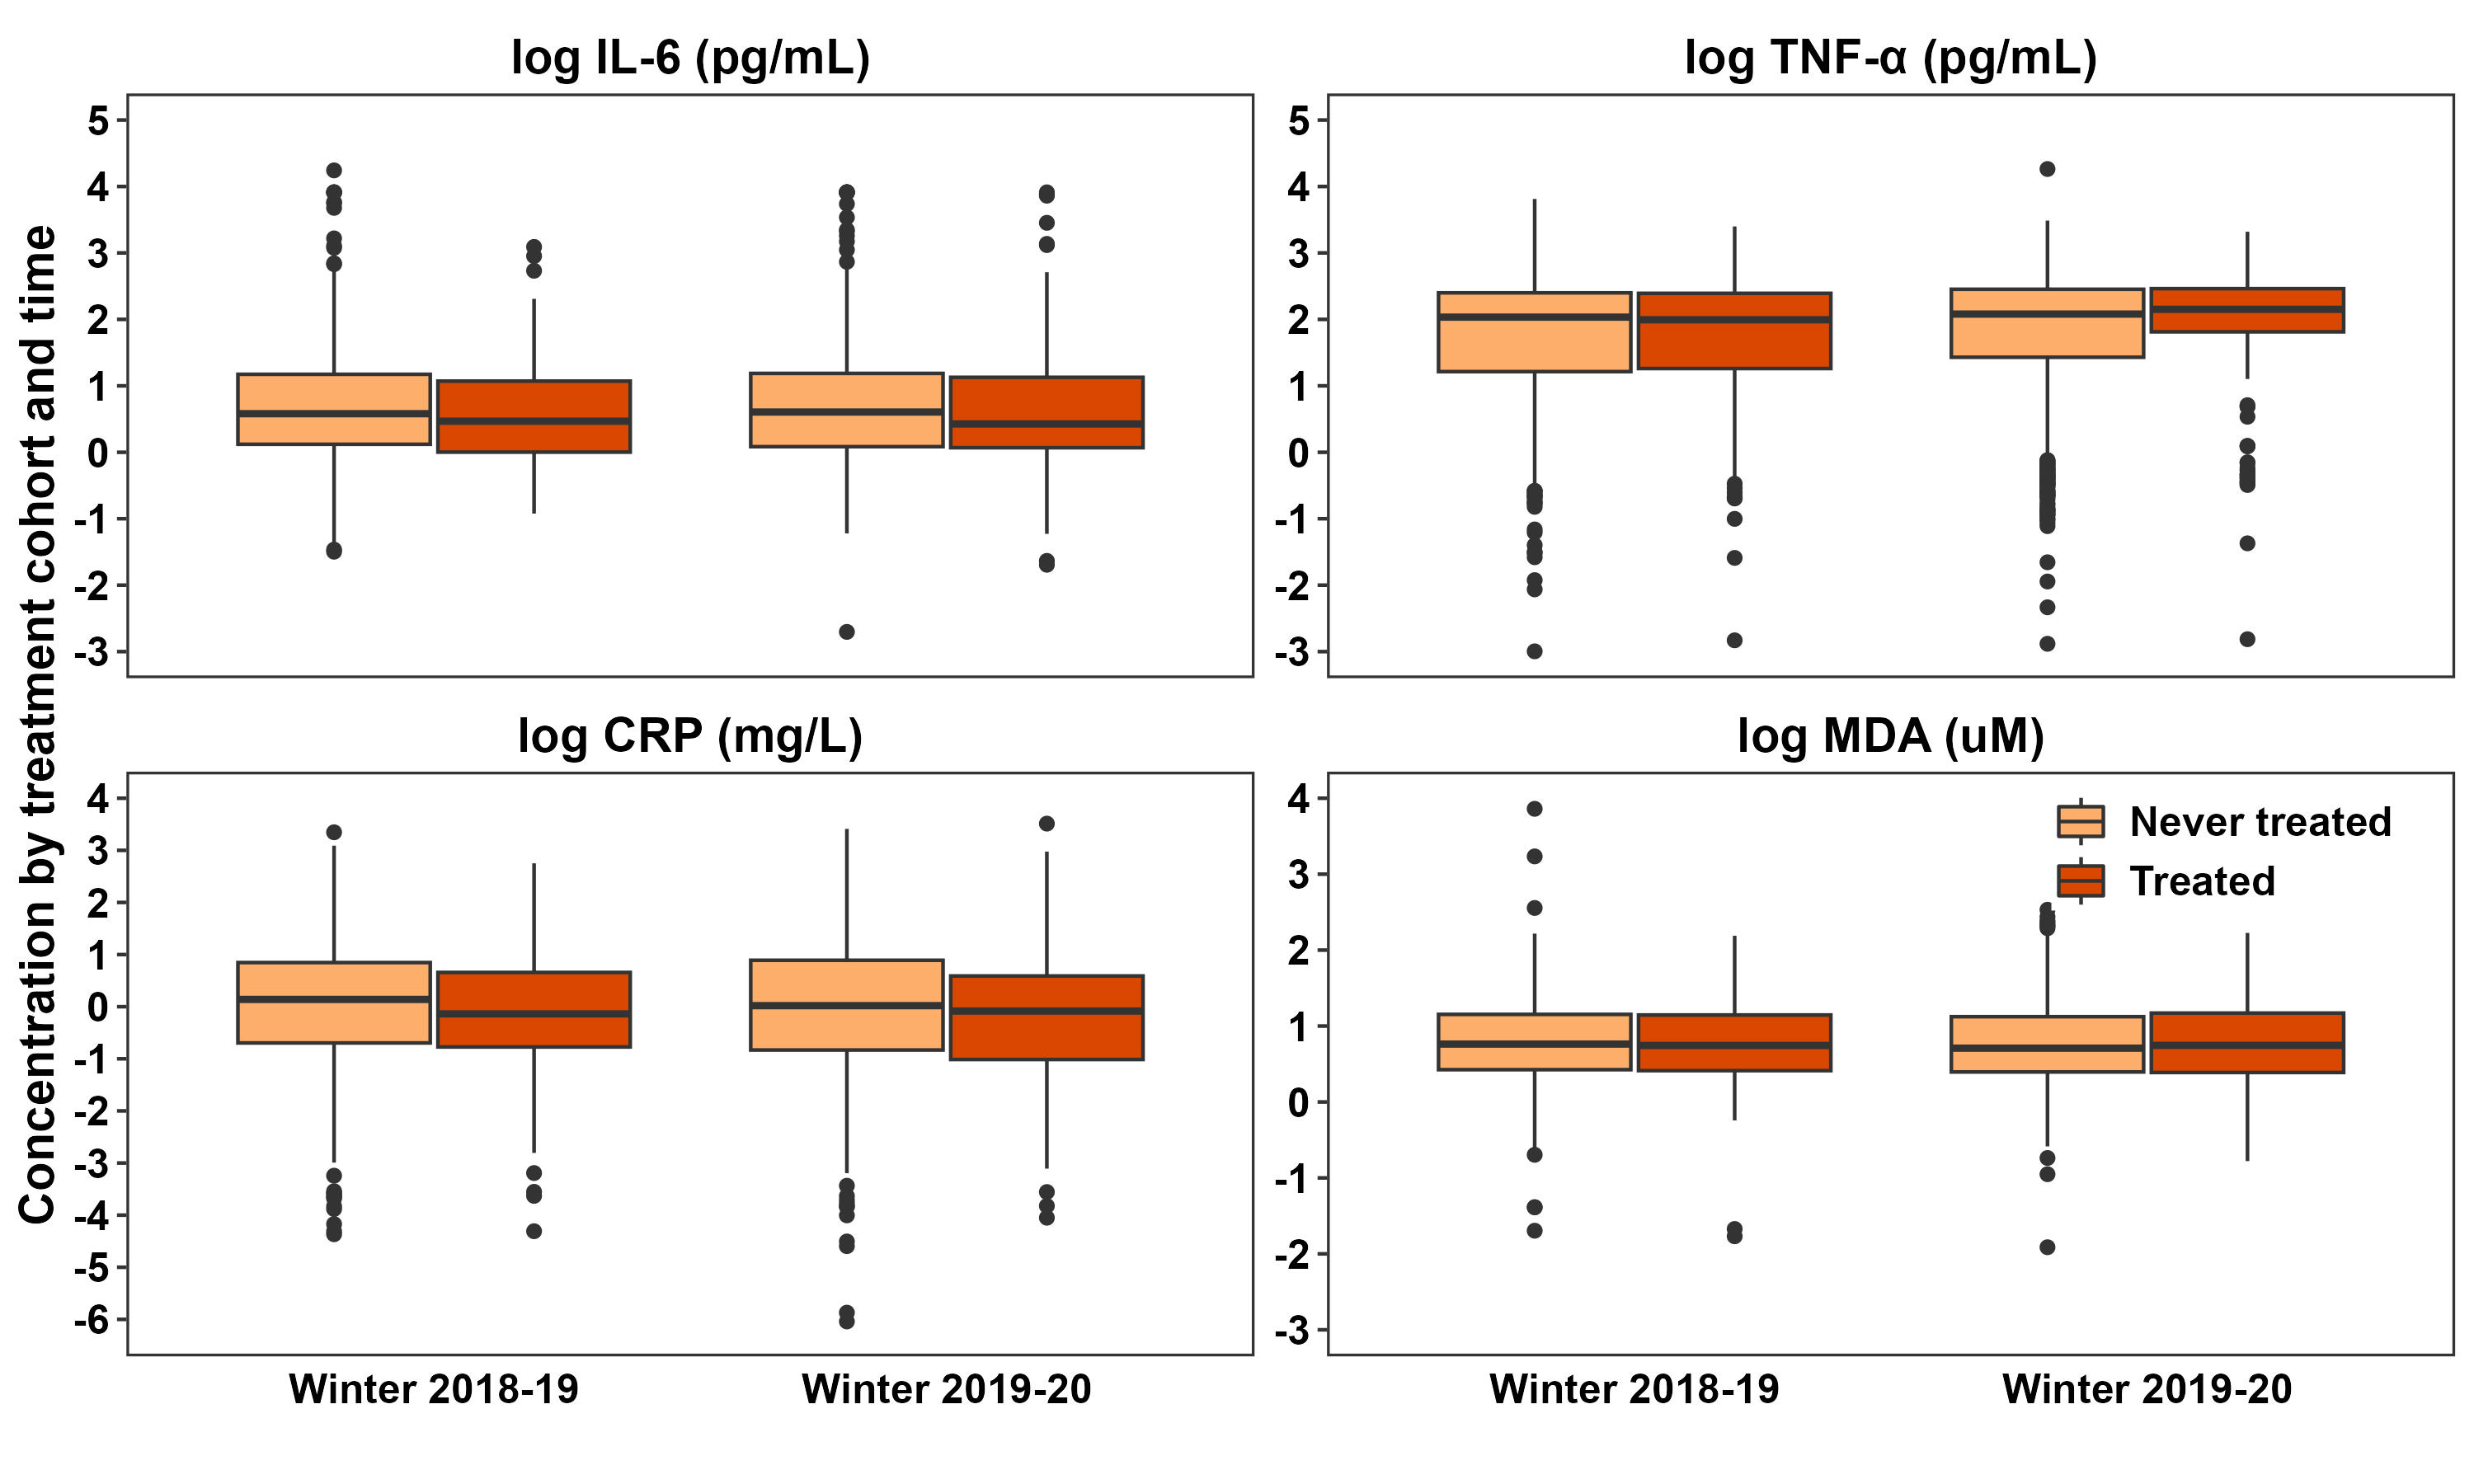
\includegraphics[width=0.9\textwidth,height=\textheight]{images/biomarker-boxplot-log.jpg}

}

\caption{\label{fig-afig-biomarkers}\DIFaddFL{Boxplots for markers of systemic
inflammation including C-reactive protein (CRP), interleukin-6 (IL-6),
tumour necrosis factor alpha (TNF-\(\alpha\)) and markers of oxidative
stress including 8-hydroxy-2'-deoxyguanosine (8-OHdG) and
malondialdehyde (MDA)}}

\end{figure}\DIFaddend %
\DIFaddbegin 

\newpage

\subsection{\DIFadd{Imputation results}}\label{imputation-results}

\DIFadd{The figures below show density plots for the values of body mass index,
waist circumference, and indoor PM\textsubscript{2.5} from the multiple
imputation models. The red lines show the values for each of the 30
imputed datasets, and the black line shows the value for the observed
data.
}

\begin{figure}[H]

\begin{minipage}[t]{0.50\linewidth}

\centering{

\captionsetup{labelsep=none}\includegraphics[width=0.5\textwidth,height=\textheight]{images/MI_BMI_density.png}

}

\subcaption{\label{fig-afig-mi-1}}

\end{minipage}%DIF > 
%DIF > 
\begin{minipage}[t]{0.50\linewidth}

\centering{

\captionsetup{labelsep=none}\includegraphics[width=0.5\textwidth,height=\textheight]{images/MI_waist_circ_density.png}

}

\subcaption{\label{fig-afig-mi-2}}

\end{minipage}%DIF > 
\newline
\begin{minipage}[t]{0.50\linewidth}

\centering{

\captionsetup{labelsep=none}\includegraphics[width=0.5\textwidth,height=\textheight]{images/MI_indoorPM_density.png}

}

\subcaption{\label{fig-afig-mi-3}}

\end{minipage}%DIF > 

\caption{\label{fig-afig-mi}\DIFaddFL{Kernal density plots showing distribution of
multiply-imputed values for body mass index (kg/m\textsuperscript{2}),
waist circumference (cm), and indoor PM\textsubscript{2.5}
(µg/m\textsuperscript{3}) (red lines) and observed values (heavy black
line)}}

\end{figure}%DIF > 

\newpage

\subsection{\DIFadd{Participant flow diagram}}\label{participant-flow-diagram}

\begin{figure}[H]

\centering{

\includegraphics[width=0.8\textwidth,height=\textheight]{images/Participation-flowchart-Apr12.png}

}

\caption{\label{fig-flowchart}\DIFaddFL{Flow chart of BHET study participation at
the participant, household, and village levels across study years.}}

\end{figure}%DIF > 

\newpage

\newpage

\subsection{\DIFadd{Policy uptake}}\label{policy-uptake-1}

\DIFadd{Figure~\ref{fig-afig-coal} shows trends over time in self-reported coal
and biomass consumption over each season. Table~\ref{tbl-fuel-did} shows
results from applying our extended two-way fixed effects models (in
separate analyses) to coal and biomass consumption.
}

\begin{figure}[H]

\centering{

\includegraphics[width=1\textwidth,height=\textheight]{images/coal-plot.png}

}

\caption{\label{fig-afig-coal}\DIFaddFL{Trends in self-reported coal and biomass,
by treatment season}}

\end{figure}%DIF > 

\begin{table}

\caption{\label{tbl-fuel-did}\DIFaddFL{Policy impacts on self-reported fuel use
(kg)}}

\centering{

}

\end{table}%DIF > 

\newpage

\subsection{\DIFadd{Heterogeneity in treament
effects}}\label{heterogeneity-in-treament-effects}

\subsubsection{\DIFadd{Personal exposure}}\label{personal-exposure}

\DIFadd{Table Table~\ref{tbl-a-het-personal} shows limited evidence that the
\(ATT\)s across cohorts and time demonstrate meaningful heterogeneity.
}

\begin{table}

\caption{\label{tbl-a-het-personal}\DIFaddFL{Heterogenous treatment effects:
Personal exposures}}

\centering{

}

\end{table}%DIF > 

\subsubsection{\texorpdfstring{Indoor
PM\textsubscript{2.5}}{Indoor PM2.5}}\label{indoor-pm2.5-1}

\DIFadd{Table Table~\ref{tbl-a-het-indoor} shows estimates for cohort-time
\(ATT\)s for daily and seasonal indoor PM\textsubscript{2.5}.
}

\begin{table}

\caption{\label{tbl-a-het-indoor}\DIFaddFL{Heterogenous treatment effects: Indoor}}

\centering{

}

\end{table}%DIF > 

\newpage

\subsubsection{\DIFadd{Indoor temperature}}\label{indoor-temperature}

\begin{table}

\caption{\label{tbl-a-het-temp}\DIFaddFL{Heterogenous treatment effects: Indoor
temperature}}

\centering{

}

\end{table}%DIF > 

\newpage

\subsubsection{\DIFadd{Blood pressure outcomes}}\label{blood-pressure-outcomes}

\DIFadd{Table~\ref{tbl-bp-het} shows \(ATT\)s by treatment cohort and time, as
well as the results of joint tests of heterogeneity across \(ATT\)s.
}

\begin{table}

\caption{\label{tbl-bp-het}\DIFaddFL{Heterogenous treatment effects for the total
effect of the CBHP policy on blood pressure.}}

\centering{

}

\end{table}%DIF > 

\newpage

\subsubsection{\DIFadd{Mediation analyses for blood
pressure}}\label{mediation-analyses-for-blood-pressure}

\DIFadd{Table~\ref{tbl-a-bp-med-het} shows the cohort-time treatment effects for
the mediation model for blood pressure.
}

\begin{table}

\caption{\label{tbl-a-bp-med-het}\DIFaddFL{Heterogenous treatment effects for
blood pressure mediation model}}

\centering{

}

\end{table}%DIF > 

\begin{table}

\caption{\label{tbl-a-bp-med-het-tests}\DIFaddFL{Heterogenous treatment effects
and tests for cohort-time heterogeneity across CDEs for multiple
mediation blood pressure mediation model.}}

\centering{

}

\end{table}%DIF > 

\newpage

\subsubsection{\DIFadd{Respiratory outcomes}}\label{respiratory-outcomes}

\DIFadd{Appendix tables \ref{tbl-a-het-resp}, \ref{tbl-a-het-cough},
\ref{tbl-a-het-phlegm}, \ref{tbl-a-het-wheeze}, \ref{tbl-a-het-breath},
\ref{tbl-a-het-nochest} below show Average Treatment Effect on the
Treated (\(ATT\)s) by treatment cohort and time. ATTs are derived from
estimating marginal effects from extended two-way fixed effects models
with additional adjustment for age, sex, and smoking status.
}

\begin{table}

\caption{\label{tbl-a-het-resp}\DIFaddFL{Heterogenous treatment effects for
self-reported respiratory outcomes: Any respiratory symptom}}

\centering{

}

\end{table}%DIF > 

\begin{table}

\caption{\label{tbl-a-het-cough}\DIFaddFL{Heterogenous treatment effects for
self-reported respiratory outcomes: Coughing}}

\centering{

}

\end{table}%DIF > 

\begin{table}

\caption{\label{tbl-a-het-phlegm}\DIFaddFL{Heterogenous treatment effects for
self-reported respiratory outcomes: Phlegm}}

\centering{

}

\end{table}%DIF > 

\begin{table}

\caption{\label{tbl-a-het-wheeze}\DIFaddFL{Heterogenous treatment effects for
self-reported respiratory outcomes: Wheezing attacks}}

\centering{

}

\end{table}%DIF > 

\begin{table}

\caption{\label{tbl-a-het-breath}\DIFaddFL{Heterogenous treatment effects for
self-reported respiratory outcomes: Trouble breathing}}

\centering{

}

\end{table}%DIF > 

\begin{table}

\caption{\label{tbl-a-het-nochest}\DIFaddFL{Heterogenous treatment effects for
self-reported respiratory outcomes: Chest trouble}}

\centering{

}

\end{table}%DIF > 

\newpage

\subsubsection{\DIFadd{Outdoor and personal mixed
combustion}}\label{outdoor-and-personal-mixed-combustion}

\begin{figure}[H]

\centering{

\includegraphics[width=1\textwidth,height=\textheight]{images/did-mixed-ct-wave.png}

}

\caption{\label{fig-afig-mixed-ct}\DIFaddFL{Adjusted and unadjusted treatment
effect for outdoor and personal exposure (µg/m\textsuperscript{3}) to
the mixed combustion source by treatment year.}}

\end{figure}%DIF > 

\newpage

\subsection{\DIFadd{Impact of sample composition on FeNO
results}}\label{impact-of-sample-composition-on-feno-results}

\DIFadd{Table~\ref{tbl-a-feno} shows differences in the \(ATT\)s for the impact
of the CBHP policy on FeNO depending on whether the estimation sample
includes all individuals or is limited to those with repeated measures
across campaigns.
}

\begin{table}

\caption{\label{tbl-a-feno}\DIFaddFL{Effects of the CBHP policy on FeNO (ppb)
based on the number of individuals with repeated measurements.}}

\centering{

}

\end{table}%DIF > 

\newpage

\subsection{\DIFadd{Impact of including Season 3
data}}\label{impact-of-including-season-3-data}

\DIFadd{Table~\ref{tbl-a-ind-s3} shows differences in the \(ATT\)s for the
impact of seasonal indoor PM\textsubscript{2.5} when season 3 data
(collected in 41 villages during COVID-19) are included versus excluded.
}

\begin{table}

\caption{\label{tbl-a-ind-s3}\DIFaddFL{Effects of the CBHP policy on indoor
seasonal PM\textsubscript{2.5} based on whether Season 3 data are
included vs.~excluded.}}

\centering{

}

\end{table}%DIF > 

\DIFadd{Figure~\ref{fig-afig-did-opm-w3} shows the impact of including Wave 3
data on the estimates of the impact of the policy on seasonal outdoor
PM\textsubscript{2.5}.
}

\begin{figure}[H]

\centering{

\includegraphics[width=0.6\textwidth,height=\textheight]{images/did-outdoor-w3.png}

}

\caption{\label{fig-afig-did-opm-w3}\DIFaddFL{Effects of the CBHP policy on
outdoor seasonal PM\textsubscript{2.5} based on whether Season 3 data
are included vs.~excluded.}}

\end{figure}%DIF > 

\newpage

\subsection{\DIFadd{Pre-trends for blood
pressure}}\label{pre-trends-for-blood-pressure}

\begin{figure}[H]

\centering{

\includegraphics[width=0.8\textwidth,height=\textheight]{images/never_Y3.png}

}

\caption{\label{fig-afig-pt3}\DIFaddFL{Comparison of pre-interventions trends in
blood pressure between waves 1 and 2 for never treated and villages
later treated in wave 3}}

\end{figure}%DIF > 

\begin{figure}[H]

\centering{

\includegraphics[width=0.7\textwidth,height=\textheight]{images/never_Y4.png}

}

\caption{\label{fig-afig-pt4}\DIFaddFL{Comparison of pre-interventions trends in
blood pressure between waves 1 and 2 for never treated and villages
later treated in wave 4}}

\end{figure}%DIF > 

\newpage

\newpage

\subsection{\DIFadd{Impact of group and time fixed
effects}}\label{impact-of-group-and-time-fixed-effects}

\begin{table}

\caption{\label{tbl-a-fe}\DIFaddFL{Effects of the CBHP policy on personal exposure
(\(\mu g / m^{3}\)) with variations in fixed effects for treatment group
and time.}}

\centering{

}

\end{table}%DIF > 

\newpage

\section*{\DIFadd{About the authors}}\label{about-the-authors}
\addcontentsline{toc}{section}{\DIFadd{About the authors}}

\section*{\DIFadd{Other publications}}\label{other-publications}
\addcontentsline{toc}{section}{\DIFadd{Other publications}}

\DIFadd{Li X, Baumgartner J, Barrington-Leigh C, Harper S, Robinson B, Shen G,
et al.~2022a. Socioeconomic and Demographic Associations with Wintertime
Air Pollution Exposures at Household, Community, and District Scales in
Rural Beijing, China. Environ Sci Technol 56:8308--8318;
doi:10.1021/acs.est.1c07402.
}

\DIFadd{Li X, Baumgartner J, Harper S, Zhang X, Sternbach T, Barrington-Leigh C,
et al.~2022b. Field measurements of indoor and community air quality in
rural Beijing before, during, and after the COVID-19 lockdown. Indoor
Air 32:e13095; doi:10.1111/ina.13095.
}

\DIFadd{Sternbach TJ, Harper S, Li X, Zhang X, Carter E, Zhang Y, et al.~2022.
Effects of indoor and outdoor temperatures on blood pressure and central
hemodynamics in a wintertime longitudinal study of Chinese adults. J
Hypertension 40:1950--1959; doi:10.1097/HJH.0000000000003198.
}

\phantomsection\label{refs}
\begin{CSLReferences}{1}{1}
\bibitem[\citeproctext]{ref-ahmed2009}
\DIFaddend Ahmed T, Dutkiewicz VA, Shareef A, Tuncel G, Tuncel S, Husain L. 2009.
Measurement of black carbon ({BC}) by an optical method and a
thermal-optical method: {Intercomparison} for four sites. Atmospheric
Environment 43:6305--6311;
doi:\href{https://doi.org/10.1016/j.atmosenv.2009.09.031}{10.1016/j.atmosenv.2009.09.031}.

\DIFdelbegin %DIFDELCMD < \leavevmode\vadjust %%%
\DIFdel{pre}%DIFDELCMD < {\hypertarget{ref-alexander2018}{}}%%%
%DIF < 
\DIFdelend \DIFaddbegin \bibitem[\citeproctext]{ref-alexander2018}
\DIFaddend Alexander DA, Northcross A, Karrison T, Morhasson-Bello O, Wilson N,
Atalabi OM, et al. 2018. Pregnancy outcomes and ethanol cook stove
intervention: {A} randomized-controlled trial in {Ibadan}, {Nigeria}.
Environment International 111:152--163;
doi:\href{https://doi.org/10.1016/j.envint.2017.11.021}{10.1016/j.envint.2017.11.021}.

\DIFdelbegin %DIFDELCMD < \leavevmode\vadjust %%%
\DIFdel{pre}%DIFDELCMD < {\hypertarget{ref-alexander2017}{}}%%%
%DIF < 
\DIFdelend \DIFaddbegin \bibitem[\citeproctext]{ref-alexander2017}
\DIFaddend Alexander D, Northcross A, Wilson N, Dutta A, Pandya R, Ibigbami T, et
al. 2017. Randomized {Controlled Ethanol Cookstove Intervention} and
{Blood Pressure} in {Pregnant Nigerian Women}. American Journal of
Respiratory and Critical Care Medicine 195:1629--1639;
doi:\href{https://doi.org/10.1164/rccm.201606-1177OC}{10.1164/rccm.201606-1177OC}.

\DIFdelbegin %DIFDELCMD < \leavevmode\vadjust %%%
\DIFdel{pre}%DIFDELCMD < {\hypertarget{ref-an2021}{}}%%%
%DIF < 
\DIFdelend \DIFaddbegin \bibitem[\citeproctext]{ref-an2021}
\DIFaddend An L, Hong B, Cui X, Geng Y, Ma X. 2021. Outdoor thermal comfort during
winter in {China}'s cold regions: {A} comparative study. Science of The
Total Environment 768:144464;
doi:\href{https://doi.org/10.1016/j.scitotenv.2020.144464}{10.1016/j.scitotenv.2020.144464}.

\DIFdelbegin %DIFDELCMD < \leavevmode\vadjust %%%
\DIFdel{pre}%DIFDELCMD < {\hypertarget{ref-anderson2016}{}}%%%
%DIF < 
\DIFdelend \DIFaddbegin \bibitem[\citeproctext]{ref-anderson2016}
\DIFaddend Anderson GB, Peng RD, Ferreri JM. 2016. Weathermetrics: {Functions} to
{Convert Between Weather Metrics}.

\DIFdelbegin %DIFDELCMD < \leavevmode\vadjust %%%
\DIFdel{pre}%DIFDELCMD < {\hypertarget{ref-archer-nicholls2016}{}}%%%
%DIF < 
\DIFdelend \DIFaddbegin \bibitem[\citeproctext]{ref-archer-nicholls2016}
\DIFaddend Archer-Nicholls S, Carter E, Kumar R, Xiao Q, Liu Y, Frostad J, et al.
2016. The {Regional Impacts} of {Cooking} and {Heating Emissions} on
{Ambient Air Quality} and {Disease Burden} in {China}. Environmental
Science \& Technology 50:9416--9423;
doi:\href{https://doi.org/10.1021/acs.est.6b02533}{10.1021/acs.est.6b02533}.

\DIFdelbegin %DIFDELCMD < \leavevmode\vadjust %%%
\DIFdel{pre}%DIFDELCMD < {\hypertarget{ref-arel-bundock2024}{}}%%%
%DIF < 
\DIFdelend \DIFaddbegin \bibitem[\citeproctext]{ref-arel-bundock2024}
\DIFaddend Arel-Bundock V. 2024. Marginaleffects: {Predictions}, {Comparisons},
{Slopes}, {Marginal Means}, and {Hypothesis Tests}.

\DIFdelbegin %DIFDELCMD < \leavevmode\vadjust %%%
\DIFdel{pre}%DIFDELCMD < {\hypertarget{ref-baker2022}{}}%%%
%DIF < 
\DIFdelend \DIFaddbegin \bibitem[\citeproctext]{ref-baker2022}
\DIFaddend Baker AC, Larcker DF, Wang CCY. 2022. How much should we trust staggered
difference-in-differences estimates? Journal of Financial Economics
144:370--395;
doi:\href{https://doi.org/10.1016/j.jfineco.2022.01.004}{10.1016/j.jfineco.2022.01.004}.

\DIFdelbegin %DIFDELCMD < \leavevmode\vadjust %%%
\DIFdel{pre}%DIFDELCMD < {\hypertarget{ref-barrington-leigh2019}{}}%%%
%DIF < 
\DIFdelend \DIFaddbegin \bibitem[\citeproctext]{ref-barrington-leigh2019}
\DIFaddend Barrington-Leigh C, Baumgartner J, Carter E, Robinson BE, Tao S, Zhang
Y. 2019. An evaluation of air quality, home heating and well-being under
{Beijing}'s programme to eliminate household coal use. Nature Energy
4:416--423;
doi:\href{https://doi.org/10.1038/s41560-019-0386-2}{10.1038/s41560-019-0386-2}.

\DIFdelbegin %DIFDELCMD < \leavevmode\vadjust %%%
\DIFdel{pre}%DIFDELCMD < {\hypertarget{ref-baumgartner2018}{}}%%%
%DIF < 
\DIFdelend \DIFaddbegin \bibitem[\citeproctext]{ref-baumgartner2018}
\DIFaddend Baumgartner J, Carter E, Schauer JJ, Ezzati M, Daskalopoulou SS, Valois
M-F, et al. 2018. Household air pollution and measures of blood
pressure, arterial stiffness and central haemodynamics. Heart
104:1515--1521;
doi:\href{https://doi.org/10.1136/heartjnl-2017-312595}{10.1136/heartjnl-2017-312595}.

\DIFdelbegin %DIFDELCMD < \leavevmode\vadjust %%%
\DIFdel{pre}%DIFDELCMD < {\hypertarget{ref-baumgartner2019}{}}%%%
%DIF < 
\DIFdelend \DIFaddbegin \bibitem[\citeproctext]{ref-baumgartner2019}
\DIFaddend Baumgartner J, Clark S, Carter E, Lai A, Zhang Y, Shan M, et al. 2019.
Effectiveness of a {Household Energy Package} in {Improving Indoor Air
Quality} and {Reducing Personal Exposures} in {Rural China}.
Environmental Science \& Technology 53:9306--9316;
doi:\href{https://doi.org/10.1021/acs.est.9b02061}{10.1021/acs.est.9b02061}.

\DIFdelbegin %DIFDELCMD < \leavevmode\vadjust %%%
\DIFdel{pre}%DIFDELCMD < {\hypertarget{ref-baumgartner2011}{}}%%%
%DIF < 
\DIFdelend \DIFaddbegin \bibitem[\citeproctext]{ref-baumgartner2011}
\DIFaddend Baumgartner J, Schauer JJ, Ezzati M, Lu L, Cheng C, Patz JA, et al.
2011. Indoor {Air Pollution} and {Blood Pressure} in {Adult Women
Living} in {Rural China}. Environmental Health Perspectives
119:1390--1395;
doi:\href{https://doi.org/10.1289/ehp.1003371}{10.1289/ehp.1003371}.

\DIFdelbegin %DIFDELCMD < \leavevmode\vadjust %%%
\DIFdel{pre}%DIFDELCMD < {\hypertarget{ref-beltramo2013}{}}%%%
%DIF < 
\DIFdelend \DIFaddbegin \bibitem[\citeproctext]{ref-beltramo2013}
\DIFaddend Beltramo T, Levine DI. 2013. The effect of solar ovens on fuel use,
emissions and health: Results from a randomised controlled trial.
Journal of Development Effectiveness 5:178--207;
doi:\href{https://doi.org/10.1080/19439342.2013.775177}{10.1080/19439342.2013.775177}.

\DIFdelbegin %DIFDELCMD < \leavevmode\vadjust %%%
\DIFdel{pre}%DIFDELCMD < {\hypertarget{ref-brauer2021}{}}%%%
%DIF < 
\DIFdelend \DIFaddbegin \bibitem[\citeproctext]{ref-brauer2021}
\DIFaddend Brauer M, Casadei B, Harrington RA, Kovacs R, Sliwa K, the WHF Air
Pollution Expert Group. 2021. Taking a {Stand Against Air
Pollution}---{The Impact} on {Cardiovascular Disease}: {A Joint Opinion
From} the {World Heart Federation}, {American College} of {Cardiology},
{American Heart Association}, and the {European Society} of
{Cardiology}. Circulation 143;
doi:\href{https://doi.org/10.1161/CIRCULATIONAHA.120.052666}{10.1161/CIRCULATIONAHA.120.052666}.

\DIFdelbegin %DIFDELCMD < \leavevmode\vadjust %%%
\DIFdel{pre}%DIFDELCMD < {\hypertarget{ref-burwen2012}{}}%%%
%DIF < 
\DIFdelend \DIFaddbegin \bibitem[\citeproctext]{ref-burwen2012}
\DIFaddend Burwen J, Levine DI. 2012. A rapid assessment randomized-controlled
trial of improved cookstoves in rural {Ghana}. Energy for Sustainable
Development 16:328--338;
doi:\href{https://doi.org/10.1016/j.esd.2012.04.001}{10.1016/j.esd.2012.04.001}.

\DIFdelbegin %DIFDELCMD < \leavevmode\vadjust %%%
\DIFdel{pre}%DIFDELCMD < {\hypertarget{ref-callaway2020}{}}%%%
%DIF < 
\DIFdelend \DIFaddbegin \bibitem[\citeproctext]{ref-callaway2020}
\DIFaddend Callaway B. 2020.
\href{https://doi.org/10.1007/978-3-319-57365-6_352-1}{Difference-in-{Differences}
for {Policy Evaluation}}. In: \emph{Handbook of {Labor}, {Human
Resources} and {Population Economics}} (K.F. Zimmermann, ed). Springer
International Publishing:Cham. 1--61.

\DIFdelbegin %DIFDELCMD < \leavevmode\vadjust %%%
\DIFdel{pre}%DIFDELCMD < {\hypertarget{ref-callaway2021}{}}%%%
%DIF < 
\DIFdelend \DIFaddbegin \bibitem[\citeproctext]{ref-callaway2021}
\DIFaddend Callaway B, Sant'Anna PHC. 2021. Difference-in-{Differences} with
multiple time periods. Journal of Econometrics 225:200--230;
doi:\href{https://doi.org/10.1016/j.jeconom.2020.12.001}{10.1016/j.jeconom.2020.12.001}.

\DIFdelbegin %DIFDELCMD < \leavevmode\vadjust %%%
\DIFdel{pre}%DIFDELCMD < {\hypertarget{ref-cameron2015}{}}%%%
%DIF < 
\DIFdelend \DIFaddbegin \bibitem[\citeproctext]{ref-cameron2015}
\DIFaddend Cameron AC, Miller DL. 2015. A practitioner's guide to cluster-robust
inference. Journal of Human Resources 50: 317--372.

\DIFdelbegin %DIFDELCMD < \leavevmode\vadjust %%%
\DIFdel{pre}%DIFDELCMD < {\hypertarget{ref-card1994}{}}%%%
%DIF < 
\DIFdelend \DIFaddbegin \bibitem[\citeproctext]{ref-card1994}
\DIFaddend Card D, Krueger AB. 1994. Minimum {Wages} and {Employment}: {A Case
Study} of the {Fast-Food Industry} in {New Jersey} and {Pennsylvania}.
American Economic Review 84: 772--93.

\DIFdelbegin %DIFDELCMD < \leavevmode\vadjust %%%
\DIFdel{pre}%DIFDELCMD < {\hypertarget{ref-chao2021}{}}%%%
%DIF < 
\DIFdelend \DIFaddbegin \bibitem[\citeproctext]{ref-chao2021}
\DIFaddend Chao C-Y, Zhang H, Hammer M, Zhan Y, Kenney D, Martin RV, et al. 2021.
Integrating {Fixed Monitoring Systems} with {Low-Cost Sensors} to
{Create High-Resolution Air Quality Maps} for the {Northern China Plain
Region}. ACS Earth and Space Chemistry 5:3022--3035;
doi:\href{https://doi.org/10.1021/acsearthspacechem.1c00174}{10.1021/acsearthspacechem.1c00174}.

\DIFdelbegin %DIFDELCMD < \leavevmode\vadjust %%%
\DIFdel{pre}%DIFDELCMD < {\hypertarget{ref-checkley2021}{}}%%%
%DIF < 
\DIFdelend \DIFaddbegin \bibitem[\citeproctext]{ref-checkley2021}
\DIFaddend Checkley W, Williams KN, Kephart JL, Fandiño-Del-Rio M, Steenland NK,
Gonzales GF, et al. 2021. Effects of a {Household Air Pollution
Intervention} with {Liquefied Petroleum Gas} on {Cardiopulmonary
Outcomes} in {Peru}. {A Randomized Controlled Trial}. American Journal
of Respiratory and Critical Care Medicine 203:1386--1397;
doi:\href{https://doi.org/10.1164/rccm.202006-2319OC}{10.1164/rccm.202006-2319OC}.

\DIFdelbegin %DIFDELCMD < \leavevmode\vadjust %%%
\DIFdel{pre}%DIFDELCMD < {\hypertarget{ref-chillrud2021}{}}%%%
%DIF < 
\DIFdelend \DIFaddbegin \bibitem[\citeproctext]{ref-chillrud2021}
\DIFaddend Chillrud SN, Ae-Ngibise KA, Gould CF, Owusu-Agyei S, Mujtaba M, Manu G,
et al. 2021. The effect of clean cooking interventions on mother and
child personal exposure to air pollution: Results from the {Ghana
Randomized Air Pollution} and {Health Study} ({GRAPHS}). Journal of
Exposure Science \& Environmental Epidemiology 31:683--698;
doi:\href{https://doi.org/10.1038/s41370-021-00309-5}{10.1038/s41370-021-00309-5}.

\DIFdelbegin %DIFDELCMD < \leavevmode\vadjust %%%
\DIFdel{pre}%DIFDELCMD < {\hypertarget{ref-clark2017}{}}%%%
%DIF < 
\DIFdelend \DIFaddbegin \bibitem[\citeproctext]{ref-clark2017}
\DIFaddend Clark S, Carter E, Shan M, Ni K, Niu H, Tseng JTW, et al. 2017. Adoption
and use of a semi-gasifier cooking and water heating stove and fuel
intervention in the {Tibetan Plateau}, {China}. Environmental Research
Letters 12:075004;
doi:\href{https://doi.org/10.1088/1748-9326/aa751e}{10.1088/1748-9326/aa751e}.

\DIFdelbegin %DIFDELCMD < \leavevmode\vadjust %%%
\DIFdel{pre}%DIFDELCMD < {\hypertarget{ref-costello2015}{}}%%%
%DIF < 
\DIFdelend \DIFaddbegin \bibitem[\citeproctext]{ref-costello2015}
\DIFaddend Costello BT, Schultz MG, Black JA, Sharman JE. 2015. Evaluation of a
{Brachial Cuff} and {Suprasystolic Waveform Algorithm Method} to
{Noninvasively Derive Central Blood Pressure}. American Journal of
Hypertension 28:480--486;
doi:\href{https://doi.org/10.1093/ajh/hpu163}{10.1093/ajh/hpu163}.

\DIFdelbegin %DIFDELCMD < \leavevmode\vadjust %%%
\DIFdel{pre}%DIFDELCMD < {\hypertarget{ref-damato2018}{}}%%%
%DIF < 
\DIFdelend \DIFaddbegin \bibitem[\citeproctext]{ref-damato2018}
\DIFaddend D'Amato M, Molino A, Calabrese G, Cecchi L, Annesi-Maesano I, D'Amato G.
2018. The impact of cold on the respiratory tract and its consequences
to respiratory health. Clinical and Translational Allergy 8:20;
doi:\href{https://doi.org/10.1186/s13601-018-0208-9}{10.1186/s13601-018-0208-9}.

\DIFdelbegin %DIFDELCMD < \leavevmode\vadjust %%%
\DIFdel{pre}%DIFDELCMD < {\hypertarget{ref-dai2020}{}}%%%
%DIF < 
\DIFdelend \DIFaddbegin \bibitem[\citeproctext]{ref-dai2020}
\DIFaddend Dai Q, Liu B, Bi X, Wu J, Liang D, Zhang Y, et al. 2020. Dispersion
{Normalized PMF Provides Insights} into the {Significant Changes} in
{Source Contributions} to {PM} {\textsubscript{2.5}} after the {COVID-19
Outbreak}. Environmental Science \& Technology 54:9917--9927;
doi:\href{https://doi.org/10.1021/acs.est.0c02776}{10.1021/acs.est.0c02776}.

\DIFdelbegin %DIFDELCMD < \leavevmode\vadjust %%%
\DIFdel{pre}%DIFDELCMD < {\hypertarget{ref-danesh2008}{}}%%%
%DIF < 
\DIFdelend \DIFaddbegin \bibitem[\citeproctext]{ref-danesh2008}
\DIFaddend Danesh J, Kaptoge S, Mann AG, Sarwar N, Wood A, Angleman SB, et al.
2008. Long-term interleukin-6 levels and subsequent risk of coronary
heart disease: Two new prospective studies and a systematic review. PLoS
medicine 5:e78;
doi:\href{https://doi.org/10.1371/journal.pmed.0050078}{10.1371/journal.pmed.0050078}.

\DIFdelbegin %DIFDELCMD < \leavevmode\vadjust %%%
\DIFdel{pre}%DIFDELCMD < {\hypertarget{ref-dart2001}{}}%%%
%DIF < 
\DIFdelend \DIFaddbegin \bibitem[\citeproctext]{ref-dart2001}
\DIFaddend Dart AM, Kingwell BA. 2001. Pulse pressure---a review of mechanisms and
clinical relevance. Journal of the American College of Cardiology
37:975--984;
doi:\href{https://doi.org/10.1016/S0735-1097(01)01108-1}{10.1016/S0735-1097(01)01108-1}.

\DIFdelbegin %DIFDELCMD < \leavevmode\vadjust %%%
\DIFdel{pre}%DIFDELCMD < {\hypertarget{ref-cdcgr2023}{}}%%%
%DIF < 
\DIFdelend \DIFaddbegin \bibitem[\citeproctext]{ref-cdcgr2023}
\DIFaddend Dispersed Coal Management Research Group
北京大学能源研究院气候变化与能源转型项目. 2023. 中国散煤综合治理研究报告
{China Dispersed Coal Governance Report}.

\DIFdelbegin %DIFDELCMD < \leavevmode\vadjust %%%
\DIFdel{pre}%DIFDELCMD < {\hypertarget{ref-dockery2013}{}}%%%
%DIF < 
\DIFdelend \DIFaddbegin \bibitem[\citeproctext]{ref-dockery2013}
\DIFaddend Dockery DW, Rich DQ, Goodman PG, Clancy L, Ohman-Strickland P, George P,
et al. 2013. \href{https://www.ncbi.nlm.nih.gov/pubmed/24024358}{Effect
of air pollution control on mortality and hospital admissions in
{Ireland}}. Research Report (Health Effects Institute) 3--109.

\DIFdelbegin %DIFDELCMD < \leavevmode\vadjust %%%
\DIFdel{pre}%DIFDELCMD < {\hypertarget{ref-dominici2014}{}}%%%
%DIF < 
\DIFdelend \DIFaddbegin \bibitem[\citeproctext]{ref-dominici2014}
\DIFaddend Dominici F, Greenstone M, Sunstein CR. 2014. Science and regulation.
{Particulate} matter matters. Science (New York, NY) 344:257--9;
doi:\href{https://doi.org/10.1126/science.1247348}{10.1126/science.1247348}.

\DIFdelbegin %DIFDELCMD < \leavevmode\vadjust %%%
\DIFdel{pre}%DIFDELCMD < {\hypertarget{ref-dong2013}{}}%%%
%DIF < 
\DIFdelend \DIFaddbegin \bibitem[\citeproctext]{ref-dong2013}
\DIFaddend Dong G-H, Qian Z(Min), Xaverius PK, Trevathan E, Maalouf S, Parker J, et
al. 2013. Association {Between Long-Term Air Pollution} and {Increased
Blood Pressure} and {Hypertension} in {China}. Hypertension 61:578--584;
doi:\href{https://doi.org/10.1161/HYPERTENSIONAHA.111.00003}{10.1161/HYPERTENSIONAHA.111.00003}.

\DIFdelbegin %DIFDELCMD < \leavevmode\vadjust %%%
\DIFdel{pre}%DIFDELCMD < {\hypertarget{ref-duan2014}{}}%%%
%DIF < 
\DIFdelend \DIFaddbegin \bibitem[\citeproctext]{ref-duan2014}
\DIFaddend Duan X, Jiang Y, Wang B, Zhao X, Shen G, Cao S, et al. 2014. Household
fuel use for cooking and heating in {China}: {Results} from the first
{Chinese Environmental Exposure-Related Human Activity Patterns Survey}
({CEERHAPS}). Applied Energy 136:692--703;
doi:\href{https://doi.org/10.1016/j.apenergy.2014.09.066}{10.1016/j.apenergy.2014.09.066}.

\DIFdelbegin %DIFDELCMD < \leavevmode\vadjust %%%
\DIFdel{pre}%DIFDELCMD < {\hypertarget{ref-edwards2004}{}}%%%
%DIF < 
\DIFdelend \DIFaddbegin \bibitem[\citeproctext]{ref-edwards2004}
\DIFaddend Edwards RD, Smith KR, Zhang J, Ma Y. 2004. Implications of changes in
household stoves and fuel use in {China}. Energy Policy 32:395--411;
doi:\href{https://doi.org/10.1016/S0301-4215(02)00309-9}{10.1016/S0301-4215(02)00309-9}.

\DIFdelbegin %DIFDELCMD < \leavevmode\vadjust %%%
\DIFdel{pre}%DIFDELCMD < {\hypertarget{ref-ERF2012}{}}%%%
%DIF < 
\DIFdelend \DIFaddbegin \bibitem[\citeproctext]{ref-ERF2012}
\DIFaddend Emerging Risk Factors Collaboration. 2012. C-reactive protein,
fibrinogen, and cardiovascular disease prediction. New England Journal
of Medicine 367: 1310--1320.

\DIFdelbegin %DIFDELCMD < \leavevmode\vadjust %%%
\DIFdel{pre}%DIFDELCMD < {\hypertarget{ref-ezzati2017}{}}%%%
%DIF < 
\DIFdelend \DIFaddbegin \bibitem[\citeproctext]{ref-ezzati2017}
\DIFaddend Ezzati M, Baumgartner JC. 2017. Household energy and health: Where next
for research and practice? Lancet (London, England) 389:130--132;
doi:\href{https://doi.org/10.1016/S0140-6736(16)32506-5}{10.1016/S0140-6736(16)32506-5}.

\DIFdelbegin %DIFDELCMD < \leavevmode\vadjust %%%
\DIFdel{pre}%DIFDELCMD < {\hypertarget{ref-fda2018}{}}%%%
%DIF < 
\DIFdelend \DIFaddbegin \bibitem[\citeproctext]{ref-fda2018}
\DIFaddend Food and Drug Administration. 2018. Bioanalytical {Method Validation
Guidance} for {Industry}.

\DIFdelbegin %DIFDELCMD < \leavevmode\vadjust %%%
\DIFdel{pre}%DIFDELCMD < {\hypertarget{ref-gbdmaps2016}{}}%%%
%DIF < 
\DIFdelend \DIFaddbegin \bibitem[\citeproctext]{ref-gbdmaps2016}
\DIFaddend GBD MAPS Working Group. 2016. Burden of disease attributable to
coal-burning and other air pollution sources in {China}.

\DIFdelbegin %DIFDELCMD < \leavevmode\vadjust %%%
\DIFdel{pre}%DIFDELCMD < {\hypertarget{ref-goin2023}{}}%%%
%DIF < 
\DIFdelend \DIFaddbegin \bibitem[\citeproctext]{ref-goin2023}
\DIFaddend Goin DE, Riddell CA. 2023. Comparing {Two-way Fixed Effects} and {New
Estimators} for {Difference-in-Differences}: {A Simulation Study} and
{Empirical Example}. Epidemiology 34:535;
doi:\href{https://doi.org/10.1097/EDE.0000000000001611}{10.1097/EDE.0000000000001611}.

\DIFdelbegin %DIFDELCMD < \leavevmode\vadjust %%%
\DIFdel{pre}%DIFDELCMD < {\hypertarget{ref-goodman-bacon2021}{}}%%%
%DIF < 
\DIFdelend \DIFaddbegin \bibitem[\citeproctext]{ref-goodman-bacon2021}
\DIFaddend Goodman-Bacon A. 2021. Difference-in-differences with variation in
treatment timing. Journal of Econometrics 225:254--277;
doi:\href{https://doi.org/10.1016/j.jeconom.2021.03.014}{10.1016/j.jeconom.2021.03.014}.

\DIFdelbegin %DIFDELCMD < \leavevmode\vadjust %%%
\DIFdel{pre}%DIFDELCMD < {\hypertarget{ref-gould2023}{}}%%%
%DIF < 
\DIFdelend \DIFaddbegin \bibitem[\citeproctext]{ref-gould2023}
\DIFaddend Gould CF, Bejarano ML, Kioumourtzoglou M-A, Lee AG, Pillarisetti A,
Schlesinger SB, et al. 2023. Widespread {Clean Cooking Fuel Scale-Up}
and under-5 {Lower Respiratory Infection Mortality}: {An Ecological
Analysis} in {Ecuador}, 1990--2019. Environmental Health Perspectives
131:037017;
doi:\href{https://doi.org/10.1289/EHP11016}{10.1289/EHP11016}.

\DIFdelbegin %DIFDELCMD < \leavevmode\vadjust %%%
\DIFdel{pre}%DIFDELCMD < {\hypertarget{ref-huang2012}{}}%%%
%DIF < 
\DIFdelend \DIFaddbegin \bibitem[\citeproctext]{ref-huang2012}
\DIFaddend Huang W, Wang G, Lu S-E, Kipen H, Wang Y, Hu M, et al. 2012.
Inflammatory and {Oxidative Stress Responses} of {Healthy Young Adults}
to {Changes} in {Air Quality} during the {Beijing Olympics}. American
Journal of Respiratory and Critical Care Medicine 186:1150--1159;
doi:\href{https://doi.org/10.1164/rccm.201205-0850OC}{10.1164/rccm.201205-0850OC}.

\DIFdelbegin %DIFDELCMD < \leavevmode\vadjust %%%
\DIFdel{pre}%DIFDELCMD < {\hypertarget{ref-johnson2022}{}}%%%
%DIF < 
\DIFdelend \DIFaddbegin \bibitem[\citeproctext]{ref-johnson2022}
\DIFaddend Johnson M, Pillarisetti A, Piedrahita R, Balakrishnan K, Peel JL,
Steenland K, et al. 2022. Exposure {Contrasts} of {Pregnant Women}
during the {Household Air Pollution Intervention Network Randomized
Controlled Trial}. Environmental Health Perspectives 130:097005;
doi:\href{https://doi.org/10.1289/EHP10295}{10.1289/EHP10295}.

\DIFdelbegin %DIFDELCMD < \leavevmode\vadjust %%%
\DIFdel{pre}%DIFDELCMD < {\hypertarget{ref-johnston2013}{}}%%%
%DIF < 
\DIFdelend \DIFaddbegin \bibitem[\citeproctext]{ref-johnston2013}
\DIFaddend Johnston FH, Hanigan IC, Henderson SB, Morgan GG. 2013. Evaluation of
interventions to reduce air pollution from biomass smoke on mortality in
{Launceston}, {Australia}: Retrospective analysis of daily mortality,
1994-2007. BMJ 346:e8446--e8446;
doi:\href{https://doi.org/10.1136/bmj.e8446}{10.1136/bmj.e8446}.

\DIFdelbegin %DIFDELCMD < \leavevmode\vadjust %%%
\DIFdel{pre}%DIFDELCMD < {\hypertarget{ref-kanagasabai2022}{}}%%%
%DIF < 
\DIFdelend \DIFaddbegin \bibitem[\citeproctext]{ref-kanagasabai2022}
\DIFaddend Kanagasabai T, Xie W, Yan L, Zhao L, Carter E, Guo D, et al. 2022.
Household {Air Pollution} and {Blood Pressure}, {Vascular Damage}, and
{Subclinical Indicators} of {Cardiovascular Disease} in {Older Chinese
Adults}. American Journal of Hypertension 35:121--131;
doi:\href{https://doi.org/10.1093/ajh/hpab141}{10.1093/ajh/hpab141}.

\DIFdelbegin %DIFDELCMD < \leavevmode\vadjust %%%
\DIFdel{pre}%DIFDELCMD < {\hypertarget{ref-kashtan2023}{}}%%%
%DIF < 
\DIFdelend \DIFaddbegin \bibitem[\citeproctext]{ref-kashtan2023}
\DIFaddend Kashtan YS, Nicholson M, Finnegan C, Ouyang Z, Lebel ED, Michanowicz DR,
et al. 2023. Gas and {Propane Combustion} from {Stoves Emits Benzene}
and {Increases Indoor Air Pollution}. Environmental Science \&
Technology 57:9653--9663;
doi:\href{https://doi.org/10.1021/acs.est.2c09289}{10.1021/acs.est.2c09289}.

\DIFdelbegin %DIFDELCMD < \leavevmode\vadjust %%%
\DIFdel{pre}%DIFDELCMD < {\hypertarget{ref-katz2020}{}}%%%
%DIF < 
\DIFdelend \DIFaddbegin \bibitem[\citeproctext]{ref-katz2020}
\DIFaddend Katz J, Tielsch JM, Khatry SK, Shrestha L, Breysse P, Zeger SL, et al.
2020. Impact of {Improved Biomass} and {Liquid Petroleum Gas Stoves} on
{Birth Outcomes} in {Rural Nepal}: {Results} of 2 {Randomized Trials}.
Global Health: Science and Practice 8:372--382;
doi:\href{https://doi.org/10.9745/GHSP-D-20-00011}{10.9745/GHSP-D-20-00011}.

\DIFdelbegin %DIFDELCMD < \leavevmode\vadjust %%%
\DIFdel{pre}%DIFDELCMD < {\hypertarget{ref-keele2015}{}}%%%
%DIF < 
\DIFdelend \DIFaddbegin \bibitem[\citeproctext]{ref-keele2015}
\DIFaddend Keele L, Tingley D, Yamamoto T. 2015. Identifying mechanisms behind
policy interventions via causal mediation analysis. Journal of Policy
Analysis and Management 34: 937--963.

\DIFdelbegin %DIFDELCMD < \leavevmode\vadjust %%%
\DIFdel{pre}%DIFDELCMD < {\hypertarget{ref-khuzestani2017}{}}%%%
%DIF < 
\DIFdelend \DIFaddbegin \bibitem[\citeproctext]{ref-khuzestani2017}
\DIFaddend Khuzestani RB, Schauer JJ, Wei Y, Zhang Y, Zhang Y. 2017. A
non-destructive optical color space sensing system to quantify elemental
and organic carbon in atmospheric particulate matter on {Teflon} and
quartz filters. Atmospheric Environment 149:84--94;
doi:\href{https://doi.org/10.1016/j.atmosenv.2016.11.002}{10.1016/j.atmosenv.2016.11.002}.

\DIFdelbegin %DIFDELCMD < \leavevmode\vadjust %%%
\DIFdel{pre}%DIFDELCMD < {\hypertarget{ref-kipen2010}{}}%%%
%DIF < 
\DIFdelend \DIFaddbegin \bibitem[\citeproctext]{ref-kipen2010}
\DIFaddend Kipen H, Rich D, Huang W, Zhu T, Wang G, Hu M, et al. 2010. Measurement
of inflammation and oxidative stress following drastic changes in air
pollution during the {Beijing Olympics}: A panel study approach. Annals
of the New York Academy of Sciences 1203:160--167;
doi:\href{https://doi.org/10.1111/j.1749-6632.2010.05638.x}{10.1111/j.1749-6632.2010.05638.x}.

\DIFdelbegin %DIFDELCMD < \leavevmode\vadjust %%%
\DIFdel{pre}%DIFDELCMD < {\hypertarget{ref-kumar2021}{}}%%%
%DIF < 
\DIFdelend \DIFaddbegin \bibitem[\citeproctext]{ref-kumar2021}
\DIFaddend Kumar N, Phillip E, Cooper H, Davis M, Langevin J, Clifford M, et al.
2021. Do improved biomass cookstove interventions improve indoor air
quality and blood pressure? {A} systematic review and meta-analysis.
Environmental Pollution 290:117997;
doi:\href{https://doi.org/10.1016/j.envpol.2021.117997}{10.1016/j.envpol.2021.117997}.

\DIFdelbegin %DIFDELCMD < \leavevmode\vadjust %%%
\DIFdel{pre}%DIFDELCMD < {\hypertarget{ref-lorange2021}{}}%%%
%DIF < 
\DIFdelend \DIFaddbegin \bibitem[\citeproctext]{ref-lorange2021}
\DIFaddend L'Orange C, Neymark G, Carter E, Volckens J. 2021. A {High-throughput},
{Robotic System} for {Analysis} of {Aerosol Sampling Filters}. Aerosol
and Air Quality Research 21:210037;
doi:\href{https://doi.org/10.4209/aaqr.210037}{10.4209/aaqr.210037}.

\DIFdelbegin %DIFDELCMD < \leavevmode\vadjust %%%
\DIFdel{pre}%DIFDELCMD < {\hypertarget{ref-lai2019}{}}%%%
%DIF < 
\DIFdelend \DIFaddbegin \bibitem[\citeproctext]{ref-lai2019}
\DIFaddend Lai. 2019. Relative contributions of household solid fuel use and
outdoor air pollution to chemical components of personal {PM2}.5
exposures. Indoor Air-international Journal of Indoor Air Quality and
Climate.

\DIFdelbegin %DIFDELCMD < \leavevmode\vadjust %%%
\DIFdel{pre}%DIFDELCMD < {\hypertarget{ref-lai2024}{}}%%%
%DIF < 
\DIFdelend \DIFaddbegin \bibitem[\citeproctext]{ref-lai2024}
\DIFaddend Lai PS, Lam NL, Gallery B, Lee AG, Adair-Rohani H, Alexander D, et al.
2024. Household {Air Pollution Interventions} to {Improve Health} in
{Low-} and {Middle-Income Countries}: {An Official American Thoracic
Society Research Statement}. American Journal of Respiratory and
Critical Care Medicine 209:909--927;
doi:\href{https://doi.org/10.1164/rccm.202402-0398ST}{10.1164/rccm.202402-0398ST}.

\DIFdelbegin %DIFDELCMD < \leavevmode\vadjust %%%
\DIFdel{pre}%DIFDELCMD < {\hypertarget{ref-lewington2012}{}}%%%
%DIF < 
\DIFdelend \DIFaddbegin \bibitem[\citeproctext]{ref-lewington2012}
\DIFaddend Lewington S, LiMing L, Sherliker P, Yu G, Millwood I, Zheng B, et al.
2012. Seasonal variation in blood pressure and its relationship with
outdoor temperature in 10 diverse regions of {China}: The {China
Kadoorie Biobank}. Journal of hypertension 30: 1383.

\DIFdelbegin %DIFDELCMD < \leavevmode\vadjust %%%
\DIFdel{pre}%DIFDELCMD < {\hypertarget{ref-li2022a}{}}%%%
%DIF < 
\DIFdelend \DIFaddbegin \bibitem[\citeproctext]{ref-li2022a}
\DIFaddend Li X, Baumgartner J, Harper S, Zhang X, Sternbach T, Barrington-Leigh C,
et al. 2022. Field measurements of indoor and community air quality in
rural {Beijing} before, during, and after the {COVID-19} lockdown.
Indoor Air 32:e13095;
doi:\href{https://doi.org/10.1111/ina.13095}{10.1111/ina.13095}.

\DIFdelbegin %DIFDELCMD < \leavevmode\vadjust %%%
\DIFdel{pre}%DIFDELCMD < {\hypertarget{ref-lindemann2017}{}}%%%
%DIF < 
\DIFdelend \DIFaddbegin \bibitem[\citeproctext]{ref-lindemann2017}
\DIFaddend Lindemann U, Stotz A, Beyer N, Oksa J, Skelton DA, Becker C, et al.
2017. Effect of indoor temperature on physical performance in older
adults during days with normal temperature and heat waves. International
journal of environmental research and public health 14;
doi:\href{https://doi.org/10.3390/ijerph14020186}{10.3390/ijerph14020186}.

\DIFdelbegin %DIFDELCMD < \leavevmode\vadjust %%%
\DIFdel{pre}%DIFDELCMD < {\hypertarget{ref-lowe2009}{}}%%%
%DIF < 
\DIFdelend \DIFaddbegin \bibitem[\citeproctext]{ref-lowe2009}
\DIFaddend Lowe A, Harrison W, El-Aklouk E, Ruygrok P, Al-Jumaily AM. 2009.
Non-invasive model-based estimation of aortic pulse pressure using
suprasystolic brachial pressure waveforms. Journal of Biomechanics
42:2111--2115;
doi:\href{https://doi.org/10.1016/j.jbiomech.2009.05.029}{10.1016/j.jbiomech.2009.05.029}.

\DIFdelbegin %DIFDELCMD < \leavevmode\vadjust %%%
\DIFdel{pre}%DIFDELCMD < {\hypertarget{ref-lv2022}{}}%%%
%DIF < 
\DIFdelend \DIFaddbegin \bibitem[\citeproctext]{ref-lv2022}
\DIFaddend Lv Y, Zhu R, Xie J, Yoshino H. 2022. Indoor environment and the blood
pressure of elderly in the cold region of {China}. Indoor and Built
Environment 31:2482--2498;
doi:\href{https://doi.org/10.1177/1420326X221109510}{10.1177/1420326X221109510}.

\DIFdelbegin %DIFDELCMD < \leavevmode\vadjust %%%
\DIFdel{pre}%DIFDELCMD < {\hypertarget{ref-mccracken2007}{}}%%%
%DIF < 
\DIFdelend \DIFaddbegin \bibitem[\citeproctext]{ref-mccracken2007}
\DIFaddend McCracken JP, Smith KR, Díaz A, Mittleman MA, Schwartz J. 2007. Chimney
{Stove Intervention} to {Reduce Long-term Wood Smoke Exposure Lowers
Blood Pressure} among {Guatemalan Women}. Environmental Health
Perspectives 115:996--1001;
doi:\href{https://doi.org/10.1289/ehp.9888}{10.1289/ehp.9888}.

\DIFdelbegin %DIFDELCMD < \leavevmode\vadjust %%%
\DIFdel{pre}%DIFDELCMD < {\hypertarget{ref-mccracken2011}{}}%%%
%DIF < 
\DIFdelend \DIFaddbegin \bibitem[\citeproctext]{ref-mccracken2011}
\DIFaddend McCracken J, Smith KR, Stone P, Díaz A, Arana B, Schwartz J. 2011.
Intervention to {Lower Household Wood Smoke Exposure} in {Guatemala
Reduces ST-Segment Depression} on {Electrocardiograms}. Environmental
Health Perspectives 119:1562--1568;
doi:\href{https://doi.org/10.1289/ehp.1002834}{10.1289/ehp.1002834}.

\DIFdelbegin %DIFDELCMD < \leavevmode\vadjust %%%
\DIFdel{pre}%DIFDELCMD < {\hypertarget{ref-mei2020}{}}%%%
%DIF < 
\DIFdelend \DIFaddbegin \bibitem[\citeproctext]{ref-mei2020}
\DIFaddend Mei H, Han P, Wang Y, Zeng N, Liu D, Cai Q, et al. 2020. Field
{Evaluation} of {Low-Cost Particulate Matter Sensors} in {Beijing}.
Sensors 20:4381;
doi:\href{https://doi.org/10.3390/s20164381}{10.3390/s20164381}.

\DIFdelbegin %DIFDELCMD < \leavevmode\vadjust %%%
\DIFdel{pre}%DIFDELCMD < {\hypertarget{ref-meng2023}{}}%%%
%DIF < 
\DIFdelend \DIFaddbegin \bibitem[\citeproctext]{ref-meng2023}
\DIFaddend Meng W, Zhu L, Liang Z, Xu H, Zhang W, Li J, et al. 2023. Significant
but {Inequitable Cost-Effective Benefits} of a {Clean Heating Campaign}
in {Northern China}. Environmental Science \& Technology 57:8467--8475;
doi:\href{https://doi.org/10.1021/acs.est.2c07492}{10.1021/acs.est.2c07492}.

\DIFdelbegin %DIFDELCMD < \leavevmode\vadjust %%%
\DIFdel{pre}%DIFDELCMD < {\hypertarget{ref-naimi2014}{}}%%%
%DIF < 
\DIFdelend \DIFaddbegin \bibitem[\citeproctext]{ref-naimi2014}
\DIFaddend Naimi AI, Kaufman JS, MacLehose RF. 2014. Mediation misgivings:
Ambiguous clinical and public health interpretations of natural direct
and indirect effects. International journal of epidemiology 43:1656--61;
doi:\href{https://doi.org/10.1093/ije/dyu107}{10.1093/ije/dyu107}.

\DIFdelbegin %DIFDELCMD < \leavevmode\vadjust %%%
\DIFdel{pre}%DIFDELCMD < {\hypertarget{ref-niu2024}{}}%%%
%DIF < 
\DIFdelend \DIFaddbegin \bibitem[\citeproctext]{ref-niu2024}
\DIFaddend Niu J, Chen X, Sun S. 2024. China's {Coal Ban} policy: {Clearing} skies,
challenging growth. Journal of Environmental Management 349:119420;
doi:\href{https://doi.org/10.1016/j.jenvman.2023.119420}{10.1016/j.jenvman.2023.119420}.

\DIFdelbegin %DIFDELCMD < \leavevmode\vadjust %%%
\DIFdel{pre}%DIFDELCMD < {\hypertarget{ref-olson2016}{}}%%%
%DIF < 
\DIFdelend \DIFaddbegin \bibitem[\citeproctext]{ref-olson2016}
\DIFaddend Olson MR, Graham E, Hamad S, Uchupalanun P, Ramanathan N, Schauer JJ.
2016. Quantification of elemental and organic carbon in atmospheric
particulate matter using color space sensing---hue, saturation, and
value ({HSV}) coordinates. Science of The Total Environment
548--549:252--259;
doi:\href{https://doi.org/10.1016/j.scitotenv.2016.01.032}{10.1016/j.scitotenv.2016.01.032}.

\DIFdelbegin %DIFDELCMD < \leavevmode\vadjust %%%
\DIFdel{pre}%DIFDELCMD < {\hypertarget{ref-onakomaiya2019}{}}%%%
%DIF < 
\DIFdelend \DIFaddbegin \bibitem[\citeproctext]{ref-onakomaiya2019}
\DIFaddend Onakomaiya D, Gyamfi J, Iwelunmor J, Opeyemi J, Oluwasanmi M,
Obiezu-Umeh C, et al. 2019. Implementation of clean cookstove
interventions and its effects on blood pressure in low-income and
middle-income countries: Systematic review. BMJ Open 9:e026517;
doi:\href{https://doi.org/10.1136/bmjopen-2018-026517}{10.1136/bmjopen-2018-026517}.

\DIFdelbegin %DIFDELCMD < \leavevmode\vadjust %%%
\DIFdel{pre}%DIFDELCMD < {\hypertarget{ref-pearl2000}{}}%%%
%DIF < 
\DIFdelend \DIFaddbegin \bibitem[\citeproctext]{ref-pearl2000}
\DIFaddend Pearl J. 2000. \emph{Causality: Models, reasoning, and inference}.
Cambridge University Press:Cambridge, U.K. ; New York.

\DIFdelbegin %DIFDELCMD < \leavevmode\vadjust %%%
\DIFdel{pre}%DIFDELCMD < {\hypertarget{ref-pearson2003}{}}%%%
%DIF < 
\DIFdelend \DIFaddbegin \bibitem[\citeproctext]{ref-pearson2003}
\DIFaddend Pearson TA, Mensah GA, Alexander RW, Anderson JL, Cannon RO 3rd, Criqui
M, et al. 2003.
\href{https://www.ncbi.nlm.nih.gov/pubmed/12551878}{Markers of
inflammation and cardiovascular disease: Application to clinical and
public health practice: {A} statement for healthcare professionals from
the {Centers} for {Disease Control} and {Prevention} and the {American
Heart Association}}. Circulation 107: 499--511.

\DIFdelbegin %DIFDELCMD < \leavevmode\vadjust %%%
\DIFdel{pre}%DIFDELCMD < {\hypertarget{ref-peel2015}{}}%%%
%DIF < 
\DIFdelend \DIFaddbegin \bibitem[\citeproctext]{ref-peel2015}
\DIFaddend Peel JL, Baumgartner J, Wellenius GA, Clark ML, Smith KR. 2015. Are
{Randomized Trials Necessary} to {Advance Epidemiologic Research} on
{Household Air Pollution}? Current Epidemiology Reports 2:263--270;
doi:\href{https://doi.org/10.1007/s40471-015-0054-4}{10.1007/s40471-015-0054-4}.

\DIFdelbegin %DIFDELCMD < \leavevmode\vadjust %%%
\DIFdel{pre}%DIFDELCMD < {\hypertarget{ref-pope2004}{}}%%%
%DIF < 
\DIFdelend \DIFaddbegin \bibitem[\citeproctext]{ref-pope2004}
\DIFaddend Pope III CA, Hansen ML, Long RW, Nielsen KR, Eatough NL, Wilson WE, et
al. 2004. Ambient particulate air pollution, heart rate variability, and
blood markers of inflammation in a panel of elderly subjects.
Environmental health perspectives 112:339--45;
doi:\href{https://doi.org/10.1289/ehp.6588}{10.1289/ehp.6588}.

\DIFdelbegin %DIFDELCMD < \leavevmode\vadjust %%%
\DIFdel{pre}%DIFDELCMD < {\hypertarget{ref-quansah2017}{}}%%%
%DIF < 
\DIFdelend \DIFaddbegin \bibitem[\citeproctext]{ref-quansah2017}
\DIFaddend Quansah R, Semple S, Ochieng CA, Juvekar S, Armah FA, Luginaah I, et al.
2017. Effectiveness of interventions to reduce household air pollution
and/or improve health in homes using solid fuel in low-and-middle income
countries: {A} systematic review and meta-analysis. Environment
International 103:73--90;
doi:\href{https://doi.org/10.1016/j.envint.2017.03.010}{10.1016/j.envint.2017.03.010}.

\DIFdelbegin %DIFDELCMD < \leavevmode\vadjust %%%
\DIFdel{pre}%DIFDELCMD < {\hypertarget{ref-rehfuess2014}{}}%%%
%DIF < 
\DIFdelend \DIFaddbegin \bibitem[\citeproctext]{ref-rehfuess2014}
\DIFaddend Rehfuess EA, Puzzolo E, Stanistreet D, Pope D, Bruce NG. 2014. Enablers
and {Barriers} to {Large-Scale Uptake} of {Improved Solid Fuel Stoves}:
{A Systematic Review}. Environmental Health Perspectives 122:120--130;
doi:\href{https://doi.org/10.1289/ehp.1306639}{10.1289/ehp.1306639}.

\DIFdelbegin %DIFDELCMD < \leavevmode\vadjust %%%
\DIFdel{pre}%DIFDELCMD < {\hypertarget{ref-rich2012}{}}%%%
%DIF < 
\DIFdelend \DIFaddbegin \bibitem[\citeproctext]{ref-rich2012}
\DIFaddend Rich DQ, Kipen HM, Huang W, Wang G, Wang Y, Zhu P, et al. 2012.
Association {Between Changes} in {Air Pollution Levels During} the
{Beijing Olympics} and {Biomarkers} of {Inflammation} and {Thrombosis}
in {Healthy Young Adults}. JAMA 307;
doi:\href{https://doi.org/10.1001/jama.2012.3488}{10.1001/jama.2012.3488}.

\DIFdelbegin %DIFDELCMD < \leavevmode\vadjust %%%
\DIFdel{pre}%DIFDELCMD < {\hypertarget{ref-ridker2001}{}}%%%
%DIF < 
\DIFdelend \DIFaddbegin \bibitem[\citeproctext]{ref-ridker2001}
\DIFaddend Ridker PM. 2001.
\href{https://www.ncbi.nlm.nih.gov/pubmed/11282915}{High-sensitivity
{C-reactive} protein: Potential adjunct for global risk assessment in
the primary prevention of cardiovascular disease}. Circulation 103:
1813--8.

\DIFdelbegin %DIFDELCMD < \leavevmode\vadjust %%%
\DIFdel{pre}%DIFDELCMD < {\hypertarget{ref-ridker2000}{}}%%%
%DIF < 
\DIFdelend \DIFaddbegin \bibitem[\citeproctext]{ref-ridker2000}
\DIFaddend Ridker PM, Hennekens CH, Buring JE, Rifai N. 2000. C-reactive protein
and other markers of inflammation in the prediction of cardiovascular
disease in women. The New England journal of medicine 342:836--43;
doi:\href{https://doi.org/10.1056/NEJM200003233421202}{10.1056/NEJM200003233421202}.

\DIFdelbegin %DIFDELCMD < \leavevmode\vadjust %%%
\DIFdel{pre}%DIFDELCMD < {\hypertarget{ref-romieu2009}{}}%%%
%DIF < 
\DIFdelend \DIFaddbegin \bibitem[\citeproctext]{ref-romieu2009}
\DIFaddend Romieu I, Riojas-Rodríguez H, Marrón-Mares AT, Schilmann A,
Perez-Padilla R, Masera O. 2009. Improved {Biomass Stove Intervention}
in {Rural Mexico}: {Impact} on the {Respiratory Health} of {Women}.
American Journal of Respiratory and Critical Care Medicine 180:649--656;
doi:\href{https://doi.org/10.1164/rccm.200810-1556OC}{10.1164/rccm.200810-1556OC}.

\DIFdelbegin %DIFDELCMD < \leavevmode\vadjust %%%
\DIFdel{pre}%DIFDELCMD < {\hypertarget{ref-rosenthal2018}{}}%%%
%DIF < 
\DIFdelend \DIFaddbegin \bibitem[\citeproctext]{ref-rosenthal2018}
\DIFaddend Rosenthal J, Quinn A, Grieshop AP, Pillarisetti A, Glass RI. 2018. Clean
cooking and the {SDGs}: {Integrated} analytical approaches to guide
energy interventions for health and environment goals. Energy for
sustainable development : the journal of the International Energy
Initiative 42:152--159;
doi:\href{https://doi.org/10.1016/j.esd.2017.11.003}{10.1016/j.esd.2017.11.003}.

\DIFdelbegin %DIFDELCMD < \leavevmode\vadjust %%%
\DIFdel{pre}%DIFDELCMD < {\hypertarget{ref-rtiinternational2009}{}}%%%
%DIF < 
\DIFdelend \DIFaddbegin \bibitem[\citeproctext]{ref-rtiinternational2009}
\DIFaddend RTI International. 2009. Standard {Operating Procedure} for the {X-Ray
Fluorescence Analysis} of {Particulate Matter Deposits} on {Teflon
Filters}: {PM Xrf Analysis}.

\DIFdelbegin %DIFDELCMD < \leavevmode\vadjust %%%
\DIFdel{pre}%DIFDELCMD < {\hypertarget{ref-rubin1987}{}}%%%
%DIF < 
\DIFdelend \DIFaddbegin \bibitem[\citeproctext]{ref-rubin1987}
\DIFaddend Rubin DB. 1987.
\emph{\href{https://doi.org/10.1002/9780470316696}{Multiple {Imputation}
for {Nonresponse} in {Surveys}}}. 1st ed. Wiley.

\DIFdelbegin %DIFDELCMD < \leavevmode\vadjust %%%
\DIFdel{pre}%DIFDELCMD < {\hypertarget{ref-ruckerl2007}{}}%%%
%DIF < 
\DIFdelend \DIFaddbegin \bibitem[\citeproctext]{ref-ruckerl2007}
\DIFaddend Rückerl R, Greven S, Ljungman P, Aalto P, Antoniades C, Bellander T, et
al. 2007. Air pollution and inflammation (interleukin-6, {C-reactive}
protein, fibrinogen) in myocardial infarction survivors. Environmental
health perspectives 115:1072--80;
doi:\href{https://doi.org/10.1289/ehp.10021}{10.1289/ehp.10021}.

\DIFdelbegin %DIFDELCMD < \leavevmode\vadjust %%%
\DIFdel{pre}%DIFDELCMD < {\hypertarget{ref-ruiz-mercado2013}{}}%%%
%DIF < 
\DIFdelend \DIFaddbegin \bibitem[\citeproctext]{ref-ruiz-mercado2013}
\DIFaddend Ruiz-Mercado I, Canuz E, Walker JL, Smith KR. 2013. Quantitative metrics
of stove adoption using {Stove Use Monitors} ({SUMs}). Biomass and
Bioenergy 57:136--148;
doi:\href{https://doi.org/10.1016/j.biombioe.2013.07.002}{10.1016/j.biombioe.2013.07.002}.

\DIFdelbegin %DIFDELCMD < \leavevmode\vadjust %%%
\DIFdel{pre}%DIFDELCMD < {\hypertarget{ref-scott2011}{}}%%%
%DIF < 
\DIFdelend \DIFaddbegin \bibitem[\citeproctext]{ref-scott2011}
\DIFaddend Scott AJ, Scarrott C. 2011. Impacts of residential heating intervention
measures on air quality and progress towards targets in {Christchurch}
and {Timaru}, {New Zealand}. Atmospheric Environment 45:2972--2980;
doi:\href{https://doi.org/10.1016/j.atmosenv.2010.09.008}{10.1016/j.atmosenv.2010.09.008}.

\DIFdelbegin %DIFDELCMD < \leavevmode\vadjust %%%
\DIFdel{pre}%DIFDELCMD < {\hypertarget{ref-shang2020}{}}%%%
%DIF < 
\DIFdelend \DIFaddbegin \bibitem[\citeproctext]{ref-shang2020}
\DIFaddend Shang J, Zhang Y, Schauer JJ, Tian J, Hua J, Han T, et al. 2020.
Associations between source-resolved {PM2}.5 and airway inflammation at
urban and rural locations in {Beijing}. Environment International
139:105635;
doi:\href{https://doi.org/10.1016/j.envint.2020.105635}{10.1016/j.envint.2020.105635}.

\DIFdelbegin %DIFDELCMD < \leavevmode\vadjust %%%
\DIFdel{pre}%DIFDELCMD < {\hypertarget{ref-shankar2020}{}}%%%
%DIF < 
\DIFdelend \DIFaddbegin \bibitem[\citeproctext]{ref-shankar2020}
\DIFaddend Shankar AV, Quinn AK, Dickinson KL, Williams KN, Masera O, Charron D, et
al. 2020. Everybody stacks: {Lessons} from household energy case studies
to inform design principles for clean energy transitions. Energy Policy
141:111468;
doi:\href{https://doi.org/10.1016/j.enpol.2020.111468}{10.1016/j.enpol.2020.111468}.

\DIFdelbegin %DIFDELCMD < \leavevmode\vadjust %%%
\DIFdel{pre}%DIFDELCMD < {\hypertarget{ref-shen2017}{}}%%%
%DIF < 
\DIFdelend \DIFaddbegin \bibitem[\citeproctext]{ref-shen2017}
\DIFaddend Shen H, Tao S, Chen Y, Ciais P, Güneralp B, Ru M, et al. 2017.
Urbanization-induced population migration has reduced ambient {PM}
{\textsubscript{2.5}} concentrations in {China}. Science Advances
3:e1700300;
doi:\href{https://doi.org/10.1126/sciadv.1700300}{10.1126/sciadv.1700300}.

\DIFdelbegin %DIFDELCMD < \leavevmode\vadjust %%%
\DIFdel{pre}%DIFDELCMD < {\hypertarget{ref-sinton2004}{}}%%%
%DIF < 
\DIFdelend \DIFaddbegin \bibitem[\citeproctext]{ref-sinton2004}
\DIFaddend Sinton JE, Smith KR, Peabody JW, Yaping L, Xiliang Z, Edwards R, et al.
2004. An assessment of programs to promote improved household stoves in
{China}. Energy for Sustainable Development 8:33--52;
doi:\href{https://doi.org/10.1016/S0973-0826(08)60465-2}{10.1016/S0973-0826(08)60465-2}.

\DIFdelbegin %DIFDELCMD < \leavevmode\vadjust %%%
\DIFdel{pre}%DIFDELCMD < {\hypertarget{ref-smith-sivertsen2009}{}}%%%
%DIF < 
\DIFdelend \DIFaddbegin \bibitem[\citeproctext]{ref-smith-sivertsen2009}
\DIFaddend Smith-Sivertsen T, Díaz E, Pope D, Lie RT, Díaz A, McCracken J, et al.
2009. Effect of {Reducing Indoor Air Pollution} on {Women}'s
{Respiratory Symptoms} and {Lung Function}: {The RESPIRE Randomized
Trial}, {Guatemala}. American Journal of Epidemiology 170:211--220;
doi:\href{https://doi.org/10.1093/aje/kwp100}{10.1093/aje/kwp100}.

\DIFdelbegin %DIFDELCMD < \leavevmode\vadjust %%%
\DIFdel{pre}%DIFDELCMD < {\hypertarget{ref-snider2018}{}}%%%
%DIF < 
\DIFdelend \DIFaddbegin \bibitem[\citeproctext]{ref-snider2018}
\DIFaddend Snider G, Carter E, Clark S, Tseng J(TzuW, Yang X, Ezzati M, et al.
2018. Impacts of stove use patterns and outdoor air quality on household
air pollution and cardiovascular mortality in southwestern {China}.
Environment International 117:116--124;
doi:\href{https://doi.org/10.1016/j.envint.2018.04.048}{10.1016/j.envint.2018.04.048}.

\DIFdelbegin %DIFDELCMD < \leavevmode\vadjust %%%
\DIFdel{pre}%DIFDELCMD < {\hypertarget{ref-song2023}{}}%%%
%DIF < 
\DIFdelend \DIFaddbegin \bibitem[\citeproctext]{ref-song2023}
\DIFaddend Song C, Liu B, Cheng K, Cole MA, Dai Q, Elliott RJR, et al. 2023.
Attribution of {Air Quality Benefits} to {Clean Winter Heating Policies}
in {China}: {Combining Machine Learning} with {Causal Inference}.
Environmental Science \& Technology 57:17707--17717;
doi:\href{https://doi.org/10.1021/acs.est.2c06800}{10.1021/acs.est.2c06800}.

\DIFdelbegin %DIFDELCMD < \leavevmode\vadjust %%%
\DIFdel{pre}%DIFDELCMD < {\hypertarget{ref-sternbach2022}{}}%%%
%DIF < 
\DIFdelend \DIFaddbegin \bibitem[\citeproctext]{ref-sternbach2022}
\DIFaddend Sternbach TJ, Harper S, Li X, Zhang X, Carter E, Zhang Y, et al. 2022.
Effects of indoor and outdoor temperatures on blood pressure and central
hemodynamics in a wintertime longitudinal study of {Chinese} adults.
Journal of Hypertension 40:1950--1959;
doi:\href{https://doi.org/10.1097/HJH.0000000000003198}{10.1097/HJH.0000000000003198}.

\DIFdelbegin %DIFDELCMD < \leavevmode\vadjust %%%
\DIFdel{pre}%DIFDELCMD < {\hypertarget{ref-sun2021}{}}%%%
%DIF < 
\DIFdelend \DIFaddbegin \bibitem[\citeproctext]{ref-sun2021}
\DIFaddend Sun L, Abraham S. 2021. Estimating dynamic treatment effects in event
studies with heterogeneous treatment effects. Journal of Econometrics
225:175--199;
doi:\href{https://doi.org/10.1016/j.jeconom.2020.09.006}{10.1016/j.jeconom.2020.09.006}.

\DIFdelbegin %DIFDELCMD < \leavevmode\vadjust %%%
\DIFdel{pre}%DIFDELCMD < {\hypertarget{ref-tan2023}{}}%%%
%DIF < 
\DIFdelend \DIFaddbegin \bibitem[\citeproctext]{ref-tan2023}
\DIFaddend Tan X, Chen G, Chen K. 2023. Clean heating and air pollution: {Evidence}
from {Northern China}. Energy Reports 9:303--313;
doi:\href{https://doi.org/10.1016/j.egyr.2022.11.166}{10.1016/j.egyr.2022.11.166}.

\DIFdelbegin %DIFDELCMD < \leavevmode\vadjust %%%
\DIFdel{pre}%DIFDELCMD < {\hypertarget{ref-thompson2019}{}}%%%
%DIF < 
\DIFdelend \DIFaddbegin \bibitem[\citeproctext]{ref-thompson2019}
\DIFaddend Thompson RJ, Li J, Weyant CL, Edwards R, Lan Q, Rothman N, et al. 2019.
Field {Emission Measurements} of {Solid Fuel Stoves} in {Yunnan}, {China
Demonstrate Dominant Causes} of {Uncertainty} in {Household Emission
Inventories}. Environmental Science \& Technology 53:3323--3330;
doi:\href{https://doi.org/10.1021/acs.est.8b07040}{10.1021/acs.est.8b07040}.

\DIFdelbegin %DIFDELCMD < \leavevmode\vadjust %%%
\DIFdel{pre}%DIFDELCMD < {\hypertarget{ref-tuck2009}{}}%%%
%DIF < 
\DIFdelend \DIFaddbegin \bibitem[\citeproctext]{ref-tuck2009}
\DIFaddend Tuck MK, Chan DW, Chia D, Godwin AK, Grizzle WE, Krueger KE, et al.
2009. Standard {Operating Procedures} for {Serum} and {Plasma
Collection}: {Early Detection Research Network Consensus Statement}
{\emph{Standard Operating Procedure Integration Working Group}}. Journal
of Proteome Research 8:113--117;
doi:\href{https://doi.org/10.1021/pr800545q}{10.1021/pr800545q}.

\DIFdelbegin %DIFDELCMD < \leavevmode\vadjust %%%
\DIFdel{pre}%DIFDELCMD < {\hypertarget{ref-vanbuuren2011}{}}%%%
%DIF < 
\DIFdelend \DIFaddbegin \bibitem[\citeproctext]{ref-vanbuuren2011}
\DIFaddend van Buuren S, Groothuis-Oudshoorn K. 2011. {\textbf{Mice}} :
{Multivariate Imputation} by {Chained Equations} in {\emph{R}}. Journal
of Statistical Software 45;
doi:\href{https://doi.org/10.18637/jss.v045.i03}{10.18637/jss.v045.i03}.

\DIFdelbegin %DIFDELCMD < \leavevmode\vadjust %%%
\DIFdel{pre}%DIFDELCMD < {\hypertarget{ref-vandonkelaar2021}{}}%%%
%DIF < 
\DIFdelend \DIFaddbegin \bibitem[\citeproctext]{ref-vandonkelaar2021}
\DIFaddend Van Donkelaar A, Hammer MS, Bindle L, Brauer M, Brook JR, Garay MJ, et
al. 2021. Monthly {Global Estimates} of {Fine Particulate Matter} and
{Their Uncertainty}. Environmental Science \& Technology
55:15287--15300;
doi:\href{https://doi.org/10.1021/acs.est.1c05309}{10.1021/acs.est.1c05309}.

\DIFdelbegin %DIFDELCMD < \leavevmode\vadjust %%%
\DIFdel{pre}%DIFDELCMD < {\hypertarget{ref-vanderweele2015}{}}%%%
%DIF < 
\DIFdelend \DIFaddbegin \bibitem[\citeproctext]{ref-vanderweele2015}
\DIFaddend VanderWeele TJ. 2015. \emph{Explanation in causal inference: Methods for
mediation and interaction}. Oxford University Press:New York.

\DIFdelbegin %DIFDELCMD < \leavevmode\vadjust %%%
\DIFdel{pre}%DIFDELCMD < {\hypertarget{ref-volckens2017}{}}%%%
%DIF < 
\DIFdelend \DIFaddbegin \bibitem[\citeproctext]{ref-volckens2017}
\DIFaddend Volckens J, Quinn C, Leith D, Mehaffy J, Henry CS, Miller-Lionberg D.
2017. Development and evaluation of an ultrasonic personal aerosol
sampler. Indoor air 27:409--416;
doi:\href{https://doi.org/10.1111/ina.12318}{10.1111/ina.12318}.

\DIFdelbegin %DIFDELCMD < \leavevmode\vadjust %%%
\DIFdel{pre}%DIFDELCMD < {\hypertarget{ref-wang2020}{}}%%%
%DIF < 
\DIFdelend \DIFaddbegin \bibitem[\citeproctext]{ref-wang2020}
\DIFaddend Wang Q, Zhao Q, Wang G, Wang B, Zhang Y, Zhang J, et al. 2020. The
association between ambient temperature and clinical visits for
inflammation-related diseases in rural areas in {China}. Environmental
Pollution 261:114128;
doi:\href{https://doi.org/10.1016/j.envpol.2020.114128}{10.1016/j.envpol.2020.114128}.

\DIFdelbegin %DIFDELCMD < \leavevmode\vadjust %%%
\DIFdel{pre}%DIFDELCMD < {\hypertarget{ref-wen2023}{}}%%%
%DIF < 
\DIFdelend \DIFaddbegin \bibitem[\citeproctext]{ref-wen2023}
\DIFaddend Wen H, Nie P, Liu M, Peng R, Guo T, Wang C, et al. 2023. Multi-health
effects of clean residential heating: {Evidences} from rural {China}'s
coal-to-gas/electricity project. Energy for Sustainable Development
73:66--75;
doi:\href{https://doi.org/10.1016/j.esd.2023.01.013}{10.1016/j.esd.2023.01.013}.

\DIFdelbegin %DIFDELCMD < \leavevmode\vadjust %%%
\DIFdel{pre}%DIFDELCMD < {\hypertarget{ref-wooldridge2021}{}}%%%
%DIF < 
\DIFdelend \DIFaddbegin \bibitem[\citeproctext]{ref-wooldridge2021}
\DIFaddend Wooldridge JM. 2021. Two-{Way Fixed Effects}, the {Two-Way Mundlak
Regression}, and {Difference-in-Differences Estimators}.;
doi:\href{https://doi.org/10.2139/ssrn.3906345}{10.2139/ssrn.3906345}.

\DIFdelbegin %DIFDELCMD < \leavevmode\vadjust %%%
\DIFdel{pre}%DIFDELCMD < {\hypertarget{ref-who2021}{}}%%%
%DIF < 
\DIFdelend \DIFaddbegin \bibitem[\citeproctext]{ref-who2021}
\DIFaddend World Health Organization. 2021. {WHO Global Air Quality Guidelines}:
{Particulate Matter PM2}.5 and {PM10}), {Ozone}, {Nitrogen Dioxide},
{Sulfur Dioxide} and {Carbon Monoxide}.

\DIFdelbegin %DIFDELCMD < \leavevmode\vadjust %%%
\DIFdel{pre}%DIFDELCMD < {\hypertarget{ref-xu2019}{}}%%%
%DIF < 
\DIFdelend \DIFaddbegin \bibitem[\citeproctext]{ref-xu2019}
\DIFaddend Xu H, Brook RD, Wang T, Song X, Feng B, Yi T, et al. 2019. Short-term
effects of ambient air pollution and outdoor temperature on biomarkers
of myocardial damage, inflammation and oxidative stress in healthy
adults. Environmental Epidemiology 3:e078;
doi:\href{https://doi.org/10.1097/EE9.0000000000000078}{10.1097/EE9.0000000000000078}.

\DIFdelbegin %DIFDELCMD < \leavevmode\vadjust %%%
\DIFdel{pre}%DIFDELCMD < {\hypertarget{ref-yan2020}{}}%%%
%DIF < 
\DIFdelend \DIFaddbegin \bibitem[\citeproctext]{ref-yan2020}
\DIFaddend Yan L, Carter E, Fu Y, Guo D, Huang P, Xie G, et al. 2020. Study
protocol: {The INTERMAP China Prospective} ({ICP}) study. Wellcome Open
Research 4:154;
doi:\href{https://doi.org/10.12688/wellcomeopenres.15470.2}{10.12688/wellcomeopenres.15470.2}.

\DIFdelbegin %DIFDELCMD < \leavevmode\vadjust %%%
\DIFdel{pre}%DIFDELCMD < {\hypertarget{ref-yangk2021}{}}%%%
%DIF < 
\DIFdelend \DIFaddbegin \bibitem[\citeproctext]{ref-yangk2021}
\DIFaddend Yang K. 2021. Power industry provides inexhaustible power for national
rejuvenation; 杨昆:电力工业为民族复兴提供不竭动力.

\DIFdelbegin %DIFDELCMD < \leavevmode\vadjust %%%
\DIFdel{pre}%DIFDELCMD < {\hypertarget{ref-yap2015}{}}%%%
%DIF < 
\DIFdelend \DIFaddbegin \bibitem[\citeproctext]{ref-yap2015}
\DIFaddend Yap P-S, Garcia C. 2015. Effectiveness of {Residential Wood-Burning
Regulation} on {Decreasing Particulate Matter Levels} and
{Hospitalizations} in the {San Joaquin Valley Air Basin}. American
Journal of Public Health 105:772--778;
doi:\href{https://doi.org/10.2105/AJPH.2014.302360}{10.2105/AJPH.2014.302360}.

\DIFdelbegin %DIFDELCMD < \leavevmode\vadjust %%%
\DIFdel{pre}%DIFDELCMD < {\hypertarget{ref-ye2022}{}}%%%
%DIF < 
\DIFdelend \DIFaddbegin \bibitem[\citeproctext]{ref-ye2022}
\DIFaddend Ye W, Steenland K, Quinn A, Liao J, Balakrishnan K, Rosa G, et al. 2022.
Effects of a {Liquefied Petroleum Gas Stove Intervention} on
{Gestational Blood Pressure}: {Intention-to-Treat} and
{Exposure-Response Findings From} the {HAPIN Trial}. Hypertension
79:1887--1898;
doi:\href{https://doi.org/10.1161/HYPERTENSIONAHA.122.19362}{10.1161/HYPERTENSIONAHA.122.19362}.

\DIFdelbegin %DIFDELCMD < \leavevmode\vadjust %%%
\DIFdel{pre}%DIFDELCMD < {\hypertarget{ref-young2015}{}}%%%
%DIF < 
\DIFdelend \DIFaddbegin \bibitem[\citeproctext]{ref-young2015}
\DIFaddend Young OR, Guttman D, Qi Y, Bachus K, Belis D, Cheng H, et al. 2015.
Institutionalized governance processes: {Comparing} environmental
problem solving in {China} and the {United States}. Global Environmental
Change 31:163--173;
doi:\href{https://doi.org/10.1016/j.gloenvcha.2015.01.010}{10.1016/j.gloenvcha.2015.01.010}.

\DIFdelbegin %DIFDELCMD < \leavevmode\vadjust %%%
\DIFdel{pre}%DIFDELCMD < {\hypertarget{ref-yu2021}{}}%%%
%DIF < 
\DIFdelend \DIFaddbegin \bibitem[\citeproctext]{ref-yu2021}
\DIFaddend Yu C, Kang J, Teng J, Long H, Fu Y. 2021. Does coal-to-gas policy reduce
air pollution? {Evidence} from a quasi-natural experiment in {China}.
Science of The Total Environment 773:144645;
doi:\href{https://doi.org/10.1016/j.scitotenv.2020.144645}{10.1016/j.scitotenv.2020.144645}.

\DIFdelbegin %DIFDELCMD < \leavevmode\vadjust %%%
\DIFdel{pre}%DIFDELCMD < {\hypertarget{ref-yun2020}{}}%%%
%DIF < 
\DIFdelend \DIFaddbegin \bibitem[\citeproctext]{ref-yun2020}
\DIFaddend Yun X, Shen G, Shen H, Meng W, Chen Y, Xu H, et al. 2020. Residential
solid fuel emissions contribute significantly to air pollution and
associated health impacts in {China}. Science Advances 6:eaba7621;
doi:\href{https://doi.org/10.1126/sciadv.aba7621}{10.1126/sciadv.aba7621}.

\DIFdelbegin %DIFDELCMD < \leavevmode\vadjust %%%
\DIFdel{pre}%DIFDELCMD < {\hypertarget{ref-zhang2007}{}}%%%
%DIF < 
\DIFdelend \DIFaddbegin \bibitem[\citeproctext]{ref-zhang2007}
\DIFaddend Zhang J(Jim), Smith KR. 2007. Household {Air Pollution} from {Coal} and
{Biomass Fuels} in {China}: {Measurements}, {Health Impacts}, and
{Interventions}. Environmental Health Perspectives 115:848--855;
doi:\href{https://doi.org/10.1289/ehp.9479}{10.1289/ehp.9479}.

\DIFdelbegin %DIFDELCMD < \leavevmode\vadjust %%%
\DIFdel{pre}%DIFDELCMD < {\hypertarget{ref-zhang2019}{}}%%%
%DIF < 
\DIFdelend \DIFaddbegin \bibitem[\citeproctext]{ref-zhang2019}
\DIFaddend Zhang Q, Zheng Y, Tong D, Shao M, Wang S, Zhang Y, et al. 2019. Drivers
of improved {PM} {\textsubscript{2.5}} air quality in {China} from 2013
to 2017. Proceedings of the National Academy of Sciences
116:24463--24469;
doi:\href{https://doi.org/10.1073/pnas.1907956116}{10.1073/pnas.1907956116}.

\DIFdelbegin %DIFDELCMD < \leavevmode\vadjust %%%
\DIFdel{pre}%DIFDELCMD < {\hypertarget{ref-zhang2023}{}}%%%
%DIF < 
\DIFdelend \DIFaddbegin \bibitem[\citeproctext]{ref-zhang2023}
\DIFaddend Zhang W, Xu H, Yu X, Li J, Zhang Y, Dai R, et al. 2023. Rigorous
{Regional Air Quality Standards} for {Substantial Health Benefits}.
Earth's Future 11:e2023EF003860;
doi:\href{https://doi.org/10.1029/2023EF003860}{10.1029/2023EF003860}.

\DIFdelbegin %DIFDELCMD < \leavevmode\vadjust %%%
\DIFdel{pre}%DIFDELCMD < {\hypertarget{ref-zhuang2009}{}}%%%
%DIF < 
\DIFdelend \DIFaddbegin \bibitem[\citeproctext]{ref-zhuang2009}
\DIFaddend Zhuang Z, Li Y, Chen B, Guo J. 2009. Chinese kang as a domestic heating
system in rural northern {China}---{A} review. Energy and Buildings
41:111--119;
doi:\href{https://doi.org/10.1016/j.enbuild.2008.07.013}{10.1016/j.enbuild.2008.07.013}.

\DIFdelbegin %DIFDELCMD < \leavevmode\vadjust %%%
\DIFdel{pre}%DIFDELCMD < {\hypertarget{ref-zigler2016}{}}%%%
%DIF < 
\DIFdelend \DIFaddbegin \bibitem[\citeproctext]{ref-zigler2016}
\DIFaddend Zigler CM, Kim C, Choirat C, Hansen JB, Wang Y, Hund L, et al. 2016.
\emph{Causal inference methods for estimating long-term health effects
of air quality regulations. {Research} report 187.} Health Effects
Institute / Health Effects Institute:Boston, MA.

\end{CSLReferences}
\DIFdelbegin %DIFDELCMD < 

%DIFDELCMD < \newpage
%DIFDELCMD < \appendix
%DIFDELCMD < \renewcommand{\thefigure}{A\arabic{figure}}
%DIFDELCMD < \renewcommand{\thetable}{A\arabic{table}}
%DIFDELCMD < \setcounter{figure}{0}
%DIFDELCMD < \setcounter{table}{0}
%DIFDELCMD < 

%DIFDELCMD < \hypertarget{appendices}{%
%DIFDELCMD < \section{Appendices}\label{appendices}}
%DIFDELCMD < 

%DIFDELCMD < \hypertarget{biomarker-descriptives}{%
%DIFDELCMD < \subsection{Biomarker descriptives}\label{biomarker-descriptives}}
%DIFDELCMD < 

%DIFDELCMD < %%%
\DIFdel{Below we show boxplots for the logged values of the blood inflammatory
and oxidative stress markers.
}%DIFDELCMD < 

%DIFDELCMD < \begin{figure}[H]
%DIFDELCMD < 

%DIFDELCMD < {\centering 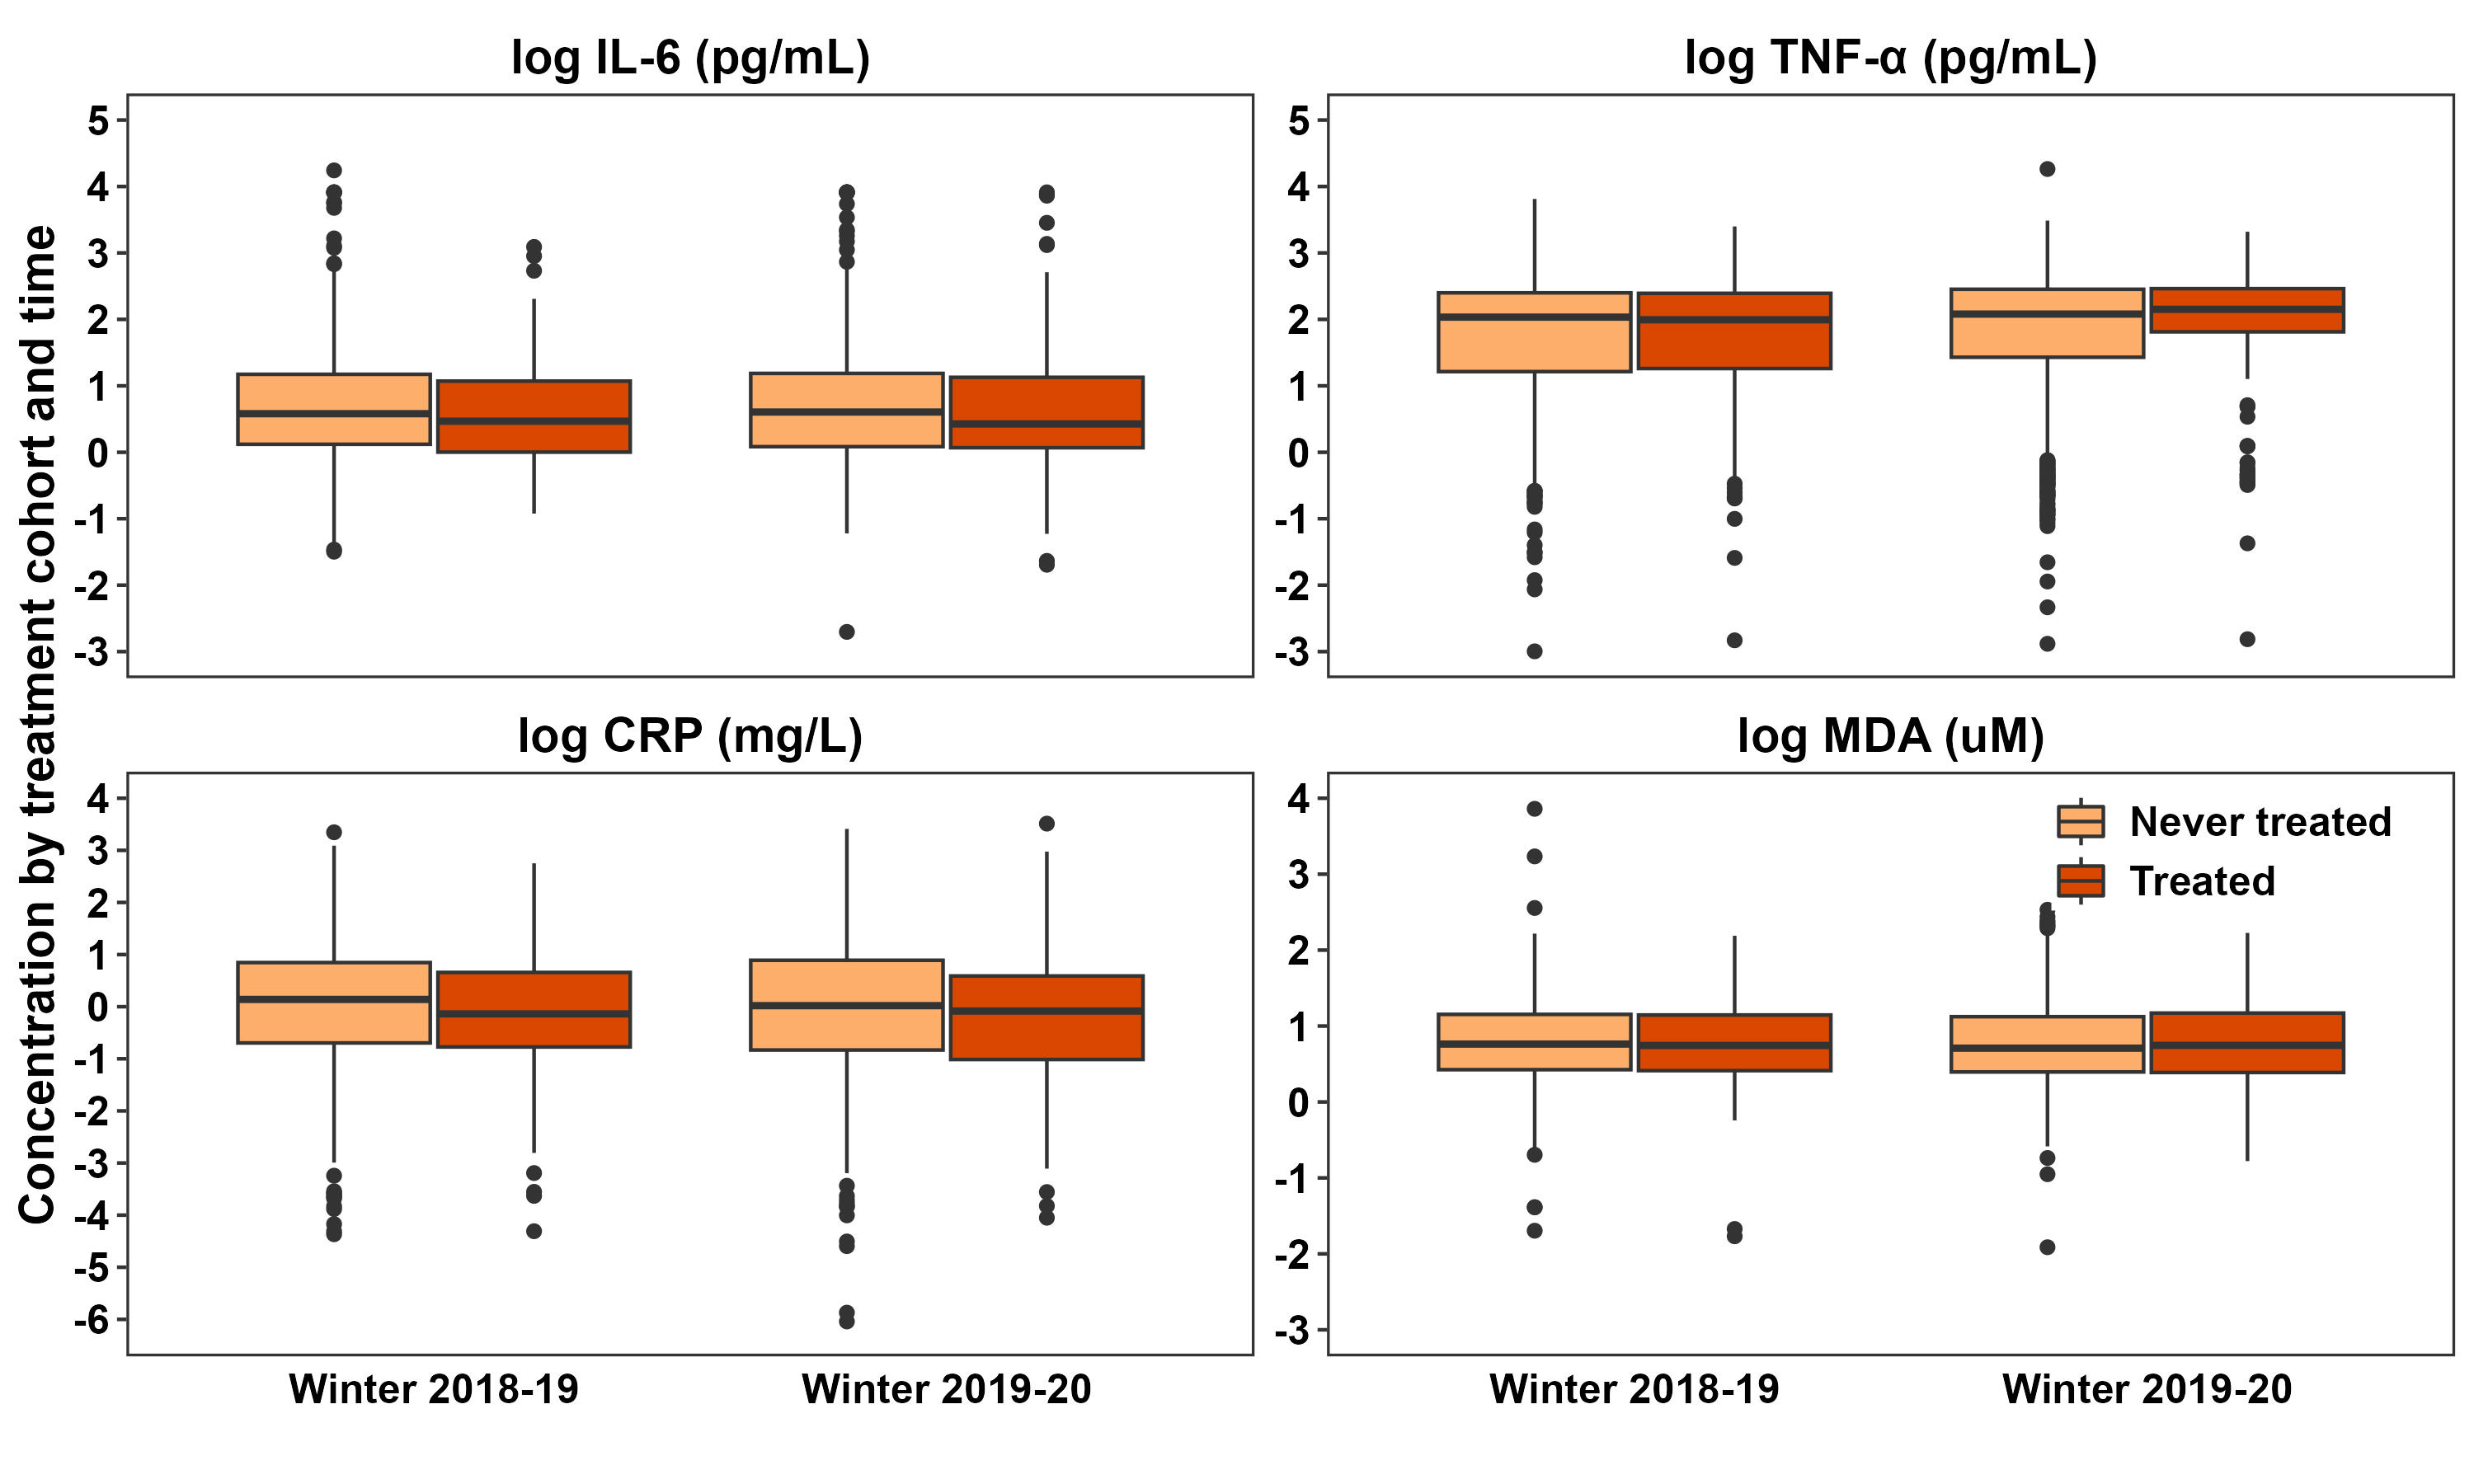
\includegraphics[width=0.9\textwidth,height=\textheight]{images/biomarker-boxplot-log.jpg}
%DIFDELCMD < 

%DIFDELCMD < }
%DIFDELCMD < 

%DIFDELCMD < %%%
%DIFDELCMD < \caption{%
{%DIFAUXCMD
%DIFDELCMD < \label{fig-afig-biomarkers}%%%
\DIFdelFL{Boxplots for markers of systemic
inflammation including C-reactive protein (CRP), interleukin-6 (IL-6),
tumour necrosis factor alpha (TNF-\(\alpha\)) and markers of oxidative
stress including 8-hydroxy-2'-deoxyguanosine (8-OHdG) and
malondialdehyde (MDA)}}
%DIFAUXCMD
%DIFDELCMD < 

%DIFDELCMD < \end{figure}
%DIFDELCMD < 

%DIFDELCMD < \newpage
%DIFDELCMD < 

%DIFDELCMD < \hypertarget{imputation-results}{%
%DIFDELCMD < \subsection{Imputation results}\label{imputation-results}}
%DIFDELCMD < 

%DIFDELCMD < %%%
\DIFdel{The figures below show density plots for the values of body mass index,
waist circumference, and indoor PM\textsubscript{2.5} from the multiple
imputation models. The red lines show the values for each of the 30
imputed datasets, and the black line shows the value for the observed
data.
}%DIFDELCMD < 

%DIFDELCMD < \begin{figure}
%DIFDELCMD < 

%DIFDELCMD < \begin{minipage}[t]{0.50\linewidth}
%DIFDELCMD < 

%DIFDELCMD < {\centering 
%DIFDELCMD < 

%DIFDELCMD < %%%
\DIFdelFL{\raisebox{-\height}{

\includegraphics{images/MI_BMI_density.png}

}
}%DIFDELCMD < 

%DIFDELCMD < }
%DIFDELCMD < 

%DIFDELCMD < %%%
%DIFDELCMD < \subcaption{%
{%DIFAUXCMD
%DIFDELCMD < \label{fig-afig-mi-1}%%%
}
%DIFAUXCMD
%DIFDELCMD < \end{minipage}%%%
%DIF < 
%DIF < 
%DIFDELCMD < \begin{minipage}[t]{0.50\linewidth}
%DIFDELCMD < 

%DIFDELCMD < {\centering 
%DIFDELCMD < 

%DIFDELCMD < %%%
\DIFdelFL{\raisebox{-\height}{

\includegraphics{images/MI_waist_circ_density.png}

}
}%DIFDELCMD < 

%DIFDELCMD < }
%DIFDELCMD < 

%DIFDELCMD < %%%
%DIFDELCMD < \subcaption{%
{%DIFAUXCMD
%DIFDELCMD < \label{fig-afig-mi-2}%%%
}
%DIFAUXCMD
%DIFDELCMD < \end{minipage}%%%
%DIF < 
%DIFDELCMD < \newline
%DIFDELCMD < \begin{minipage}[t]{0.50\linewidth}
%DIFDELCMD < 

%DIFDELCMD < {\centering 
%DIFDELCMD < 

%DIFDELCMD < %%%
\DIFdelFL{\raisebox{-\height}{

\includegraphics{images/MI_indoorPM_density.png}

}
}%DIFDELCMD < 

%DIFDELCMD < }
%DIFDELCMD < 

%DIFDELCMD < %%%
%DIFDELCMD < \subcaption{%
{%DIFAUXCMD
%DIFDELCMD < \label{fig-afig-mi-3}%%%
}
%DIFAUXCMD
%DIFDELCMD < \end{minipage}%%%
%DIF < 
%DIFDELCMD < 

%DIFDELCMD < %%%
%DIFDELCMD < \caption{%
{%DIFAUXCMD
%DIFDELCMD < \label{fig-afig-mi}%%%
\DIFdelFL{Kernal density plots showing distribution of
multiply-imputed values for body mass index (kg/m\textsuperscript{2}),
waist circumference (cm), and indoor PM\textsubscript{2.5}
(µg/m\textsuperscript{3}) (red lines) and observed values (heavy black
line)}}
%DIFAUXCMD
%DIFDELCMD < 

%DIFDELCMD < \end{figure}
%DIFDELCMD < 

%DIFDELCMD < \newpage
%DIFDELCMD < 

%DIFDELCMD < \hypertarget{participant-flow-diagram}{%
%DIFDELCMD < \subsection{Participant flow diagram}\label{participant-flow-diagram}}
%DIFDELCMD < 

%DIFDELCMD < \begin{figure}[H]
%DIFDELCMD < 

%DIFDELCMD < {\centering \includegraphics[width=0.8\textwidth,height=\textheight]{images/Participation-flowchart-Apr12.png}
%DIFDELCMD < 

%DIFDELCMD < }
%DIFDELCMD < 

%DIFDELCMD < %%%
%DIFDELCMD < \caption{%
{%DIFAUXCMD
%DIFDELCMD < \label{fig-flowchart}%%%
\DIFdelFL{Flow chart of BHET study participation at
the participant, household, and village levels across study years.}}
%DIFAUXCMD
%DIFDELCMD < 

%DIFDELCMD < \end{figure}
%DIFDELCMD < 

%DIFDELCMD < \newpage
%DIFDELCMD < 

%DIFDELCMD < \newpage
%DIFDELCMD < 

%DIFDELCMD < \hypertarget{policy-uptake-1}{%
%DIFDELCMD < \subsection{Policy uptake}\label{policy-uptake-1}}
%DIFDELCMD < 

%DIFDELCMD < %%%
\DIFdel{Figure~\ref{fig-afig-coal} shows trends over time in self-reported coal
and biomass consumption over each season. Table~\ref{tbl-fuel-did} shows
results from applying our extended two-way fixed effects models (in
separate analyses) to coal and biomass consumption.
}%DIFDELCMD < 

%DIFDELCMD < \begin{figure}[H]
%DIFDELCMD < 

%DIFDELCMD < {\centering \includegraphics[width=1\textwidth,height=\textheight]{images/coal-plot.png}
%DIFDELCMD < 

%DIFDELCMD < }
%DIFDELCMD < 

%DIFDELCMD < %%%
%DIFDELCMD < \caption{%
{%DIFAUXCMD
%DIFDELCMD < \label{fig-afig-coal}%%%
\DIFdelFL{Trends in self-reported coal and biomass,
by treatment season}}
%DIFAUXCMD
%DIFDELCMD < 

%DIFDELCMD < \end{figure}
%DIFDELCMD < 

%DIFDELCMD < \hypertarget{tbl-fuel-did}{}
%DIFDELCMD < \begin{table}[H]
%DIFDELCMD < %%%
%DIFDELCMD < \caption{%
{%DIFAUXCMD
%DIFDELCMD < \label{tbl-fuel-did}%%%
\DIFdelFL{Policy impacts on self-reported fuel use (kg) }}%DIFAUXCMD
%DIFDELCMD < \tabularnewline
%DIFDELCMD < 

%DIFDELCMD < \centering
%DIFDELCMD < \begin{tabular}{>{\centering\arraybackslash}p{1.5cm}>{\centering\arraybackslash}p{1.5cm}cccc}
%DIFDELCMD < \toprule
%DIFDELCMD < \multicolumn{2}{c}{ } & \multicolumn{2}{c}{Coal\textsuperscript{a}} & \multicolumn{2}{c}{Biomass\textsuperscript{b}} \\
%DIFDELCMD < \cmidrule%%%
\DIFdelFL{(l}%DIFDELCMD < {%%%
\DIFdelFL{3pt}%DIFDELCMD < }%%%
\DIFdelFL{r}%DIFDELCMD < {%%%
\DIFdelFL{3pt}%DIFDELCMD < }%%%
\DIFdelFL{)}%DIFDELCMD < {%%%
\DIFdelFL{3-4}%DIFDELCMD < } \cmidrule%%%
\DIFdelFL{(l}%DIFDELCMD < {%%%
\DIFdelFL{3pt}%DIFDELCMD < }%%%
\DIFdelFL{r}%DIFDELCMD < {%%%
\DIFdelFL{3pt}%DIFDELCMD < }%%%
\DIFdelFL{)}%DIFDELCMD < {%%%
\DIFdelFL{5-6}%DIFDELCMD < }
%DIFDELCMD < %%%
\DIFdelFL{Cohort }%DIFDELCMD < & %%%
\DIFdelFL{Time }%DIFDELCMD < & %%%
\DIFdelFL{ATT }%DIFDELCMD < & %%%
\DIFdelFL{(95\%CI) }%DIFDELCMD < & %%%
\DIFdelFL{ATT }%DIFDELCMD < & %%%
\DIFdelFL{(95\%CI)}%DIFDELCMD < \\
%DIFDELCMD < \midrule
%DIFDELCMD < \addlinespace[0.3em]
%DIFDELCMD < \multicolumn{6}{l}{\textbf{Average ATT}}\\
%DIFDELCMD < %%%
\DIFdelFL{All }%DIFDELCMD < & %%%
\DIFdelFL{All }%DIFDELCMD < & %%%
\DIFdelFL{-2361 }%DIFDELCMD < & %%%
\DIFdelFL{(-2677, -2044) }%DIFDELCMD < & %%%
\DIFdelFL{-487 }%DIFDELCMD < & %%%
\DIFdelFL{(-805, -168)}%DIFDELCMD < \\
%DIFDELCMD < \addlinespace[0.3em]
%DIFDELCMD < \multicolumn{6}{l}{\textbf{Cohort-Time ATTs}}\\
%DIFDELCMD < %%%
\DIFdelFL{2019 }%DIFDELCMD < & %%%
\DIFdelFL{2019 }%DIFDELCMD < & %%%
\DIFdelFL{-2631 }%DIFDELCMD < & %%%
\DIFdelFL{(-2913, -2348) }%DIFDELCMD < & %%%
\DIFdelFL{-653 }%DIFDELCMD < & %%%
\DIFdelFL{(-991, -315)}%DIFDELCMD < \\
%DIFDELCMD < %%%
\DIFdelFL{2019 }%DIFDELCMD < & %%%
\DIFdelFL{2021 }%DIFDELCMD < & %%%
\DIFdelFL{-2416 }%DIFDELCMD < & %%%
\DIFdelFL{(-2847, -1984) }%DIFDELCMD < & %%%
\DIFdelFL{-633 }%DIFDELCMD < & %%%
\DIFdelFL{(-1201, -64)}%DIFDELCMD < \\
%DIFDELCMD < %%%
\DIFdelFL{2020 }%DIFDELCMD < & %%%
\DIFdelFL{2021 }%DIFDELCMD < & %%%
\DIFdelFL{-2018 }%DIFDELCMD < & %%%
\DIFdelFL{(-2474, -1562) }%DIFDELCMD < & %%%
\DIFdelFL{-350 }%DIFDELCMD < & %%%
\DIFdelFL{(-701, 0)}%DIFDELCMD < \\
%DIFDELCMD < %%%
\DIFdelFL{2021 }%DIFDELCMD < & %%%
\DIFdelFL{2021 }%DIFDELCMD < & %%%
\DIFdelFL{-1961 }%DIFDELCMD < & %%%
\DIFdelFL{(-2895, -1027) }%DIFDELCMD < & %%%
\DIFdelFL{338 }%DIFDELCMD < & %%%
\DIFdelFL{(-30, 705)}%DIFDELCMD < \\
%DIFDELCMD < \bottomrule
%DIFDELCMD < \multicolumn{6}{l}{\rule{0pt}{1em}\textsuperscript{a} Joint test that all ATTs are equal: F(3, 2886)= 1.856, p= 0.135}\\
%DIFDELCMD < \multicolumn{6}{l}{\rule{0pt}{1em}\textsuperscript{b} Joint test that all ATTs are equal: F(3, 2886)= 5.545, p= 0.001}\\
%DIFDELCMD < \end{tabular}
%DIFDELCMD < \end{table}
%DIFDELCMD < 

%DIFDELCMD < \newpage
%DIFDELCMD < 

%DIFDELCMD < \hypertarget{heterogeneity-in-treament-effects}{%
%DIFDELCMD < \subsection{Heterogeneity in treament
%DIFDELCMD < effects}\label{heterogeneity-in-treament-effects}}
%DIFDELCMD < 

%DIFDELCMD < \hypertarget{personal-exposure}{%
%DIFDELCMD < \subsubsection{Personal exposure}\label{personal-exposure}}
%DIFDELCMD < 

%DIFDELCMD < %%%
\DIFdel{Table Table~\ref{tbl-a-het-personal} shows limited evidence that the
\(ATT\)s across cohorts and time demonstrate meaningful heterogeneity.
}%DIFDELCMD < 

%DIFDELCMD < \hypertarget{tbl-a-het-personal}{}
%DIFDELCMD < \begin{table}[H]
%DIFDELCMD < %%%
%DIFDELCMD < \caption{%
{%DIFAUXCMD
%DIFDELCMD < \label{tbl-a-het-personal}%%%
\DIFdelFL{Heterogenous treatment effects: Personal exposures }}%DIFAUXCMD
%DIFDELCMD < \tabularnewline
%DIFDELCMD < 

%DIFDELCMD < \centering
%DIFDELCMD < \begin{tabular}{>{\centering\arraybackslash}p{1.5cm}>{\centering\arraybackslash}p{1.5cm}cccc}
%DIFDELCMD < \toprule
%DIFDELCMD < \multicolumn{2}{c}{ } & \multicolumn{2}{c}{PM2.5\textsuperscript{a}} & \multicolumn{2}{c}{Black carbon\textsuperscript{b}} \\
%DIFDELCMD < \cmidrule%%%
\DIFdelFL{(l}%DIFDELCMD < {%%%
\DIFdelFL{3pt}%DIFDELCMD < }%%%
\DIFdelFL{r}%DIFDELCMD < {%%%
\DIFdelFL{3pt}%DIFDELCMD < }%%%
\DIFdelFL{)}%DIFDELCMD < {%%%
\DIFdelFL{3-4}%DIFDELCMD < } \cmidrule%%%
\DIFdelFL{(l}%DIFDELCMD < {%%%
\DIFdelFL{3pt}%DIFDELCMD < }%%%
\DIFdelFL{r}%DIFDELCMD < {%%%
\DIFdelFL{3pt}%DIFDELCMD < }%%%
\DIFdelFL{)}%DIFDELCMD < {%%%
\DIFdelFL{5-6}%DIFDELCMD < }
%DIFDELCMD < %%%
\DIFdelFL{Cohort }%DIFDELCMD < & %%%
\DIFdelFL{Time }%DIFDELCMD < & %%%
\DIFdelFL{ATT }%DIFDELCMD < & %%%
\DIFdelFL{(95\%CI) }%DIFDELCMD < & %%%
\DIFdelFL{ATT }%DIFDELCMD < & %%%
\DIFdelFL{(95\%CI)}%DIFDELCMD < \\
%DIFDELCMD < \midrule
%DIFDELCMD < \addlinespace[0.3em]
%DIFDELCMD < \multicolumn{6}{l}{\textbf{Average ATT}}\\
%DIFDELCMD < %%%
\DIFdelFL{All }%DIFDELCMD < & %%%
\DIFdelFL{All }%DIFDELCMD < & %%%
\DIFdelFL{1.95 }%DIFDELCMD < & %%%
\DIFdelFL{(-23.34, 27.23) }%DIFDELCMD < & %%%
\DIFdelFL{-0.43 }%DIFDELCMD < & %%%
\DIFdelFL{(-1.67, 0.81)}%DIFDELCMD < \\
%DIFDELCMD < \addlinespace[0.3em]
%DIFDELCMD < \multicolumn{6}{l}{\textbf{Cohort-Time ATTs}}\\
%DIFDELCMD < %%%
\DIFdelFL{2019 }%DIFDELCMD < & %%%
\DIFdelFL{2019 }%DIFDELCMD < & %%%
\DIFdelFL{-0.05 }%DIFDELCMD < & %%%
\DIFdelFL{(-28.97, 28.87) }%DIFDELCMD < & %%%
\DIFdelFL{-0.69 }%DIFDELCMD < & %%%
\DIFdelFL{(-1.84, 0.45)}%DIFDELCMD < \\
%DIFDELCMD < %%%
\DIFdelFL{2019 }%DIFDELCMD < & %%%
\DIFdelFL{2021 }%DIFDELCMD < & %%%
\DIFdelFL{-4.31 }%DIFDELCMD < & %%%
\DIFdelFL{(-41.92, 33.3) }%DIFDELCMD < & %%%
\DIFdelFL{-0.25 }%DIFDELCMD < & %%%
\DIFdelFL{(-2.11, 1.62)}%DIFDELCMD < \\
%DIFDELCMD < %%%
\DIFdelFL{2020 }%DIFDELCMD < & %%%
\DIFdelFL{2021 }%DIFDELCMD < & %%%
\DIFdelFL{23.61 }%DIFDELCMD < & %%%
\DIFdelFL{(-19.88, 67.11) }%DIFDELCMD < & %%%
\DIFdelFL{-0.27 }%DIFDELCMD < & %%%
\DIFdelFL{(-2.04, 1.5)}%DIFDELCMD < \\
%DIFDELCMD < %%%
\DIFdelFL{2021 }%DIFDELCMD < & %%%
\DIFdelFL{2021 }%DIFDELCMD < & %%%
\DIFdelFL{-19.06 }%DIFDELCMD < & %%%
\DIFdelFL{(-43.19, 5.07) }%DIFDELCMD < & %%%
\DIFdelFL{-0.56 }%DIFDELCMD < & %%%
\DIFdelFL{(-2.46, 1.34)}%DIFDELCMD < \\
%DIFDELCMD < \bottomrule
%DIFDELCMD < \multicolumn{6}{l}{\rule{0pt}{1em}\textsuperscript{a} Joint test that all ATTs are equal: F(3, 1271)= 0.431, p= 0.731}\\
%DIFDELCMD < \multicolumn{6}{l}{\rule{0pt}{1em}\textsuperscript{b} Joint test that all ATTs are equal: F(3, 1253)= 0.613, p= 0.607}\\
%DIFDELCMD < \end{tabular}
%DIFDELCMD < \end{table}
%DIFDELCMD < 

%DIFDELCMD < \hypertarget{indoor-pm2.5-1}{%
%DIFDELCMD < \subsubsection{\texorpdfstring{Indoor
%DIFDELCMD < PM\textsubscript{2.5}}{Indoor PM2.5}}\label{indoor-pm2.5-1}}
%DIFDELCMD < 

%DIFDELCMD < %%%
\DIFdel{Table Table~\ref{tbl-a-het-indoor} shows estimates for cohort-time
\(ATT\)s for daily and seasonal indoor PM\textsubscript{2.5}.
}%DIFDELCMD < 

%DIFDELCMD < \hypertarget{tbl-a-het-indoor}{}
%DIFDELCMD < \begin{table}[H]
%DIFDELCMD < %%%
%DIFDELCMD < \caption{%
{%DIFAUXCMD
%DIFDELCMD < \label{tbl-a-het-indoor}%%%
\DIFdelFL{Heterogenous treatment effects: Indoor }}%DIFAUXCMD
%DIFDELCMD < \tabularnewline
%DIFDELCMD < 

%DIFDELCMD < \centering
%DIFDELCMD < \begin{tabular}{>{\centering\arraybackslash}p{1.5cm}>{\centering\arraybackslash}p{1.5cm}cccc}
%DIFDELCMD < \toprule
%DIFDELCMD < \multicolumn{2}{c}{ } & \multicolumn{2}{c}{Daily\textsuperscript{a}} & \multicolumn{2}{c}{Seasonal\textsuperscript{b}} \\
%DIFDELCMD < \cmidrule%%%
\DIFdelFL{(l}%DIFDELCMD < {%%%
\DIFdelFL{3pt}%DIFDELCMD < }%%%
\DIFdelFL{r}%DIFDELCMD < {%%%
\DIFdelFL{3pt}%DIFDELCMD < }%%%
\DIFdelFL{)}%DIFDELCMD < {%%%
\DIFdelFL{3-4}%DIFDELCMD < } \cmidrule%%%
\DIFdelFL{(l}%DIFDELCMD < {%%%
\DIFdelFL{3pt}%DIFDELCMD < }%%%
\DIFdelFL{r}%DIFDELCMD < {%%%
\DIFdelFL{3pt}%DIFDELCMD < }%%%
\DIFdelFL{)}%DIFDELCMD < {%%%
\DIFdelFL{5-6}%DIFDELCMD < }
%DIFDELCMD < %%%
\DIFdelFL{Cohort }%DIFDELCMD < & %%%
\DIFdelFL{Time }%DIFDELCMD < & %%%
\DIFdelFL{ATT }%DIFDELCMD < & %%%
\DIFdelFL{(95\%CI) }%DIFDELCMD < & %%%
\DIFdelFL{ATT }%DIFDELCMD < & %%%
\DIFdelFL{(95\%CI)}%DIFDELCMD < \\
%DIFDELCMD < \midrule
%DIFDELCMD < \addlinespace[0.3em]
%DIFDELCMD < \multicolumn{6}{l}{\textbf{Average ATT}}\\
%DIFDELCMD < %%%
\DIFdelFL{All }%DIFDELCMD < & %%%
\DIFdelFL{All }%DIFDELCMD < & %%%
\DIFdelFL{-14.20 }%DIFDELCMD < & %%%
\DIFdelFL{(-53.94, 25.54) }%DIFDELCMD < & %%%
\DIFdelFL{-36.19 }%DIFDELCMD < & %%%
\DIFdelFL{(-60.74, -11.65)}%DIFDELCMD < \\
%DIFDELCMD < \addlinespace[0.3em]
%DIFDELCMD < \multicolumn{6}{l}{\textbf{Cohort-Time ATTs}}\\
%DIFDELCMD < %%%
\DIFdelFL{2020 }%DIFDELCMD < & %%%
\DIFdelFL{2021 }%DIFDELCMD < & %%%
\DIFdelFL{-4.71 }%DIFDELCMD < & %%%
\DIFdelFL{(-56.93, 47.5) }%DIFDELCMD < & %%%
\DIFdelFL{-25.44 }%DIFDELCMD < & %%%
\DIFdelFL{(-58.02, 7.13)}%DIFDELCMD < \\
%DIFDELCMD < %%%
\DIFdelFL{2021 }%DIFDELCMD < & %%%
\DIFdelFL{2021 }%DIFDELCMD < & %%%
\DIFdelFL{-37.24 }%DIFDELCMD < & %%%
\DIFdelFL{(-74.15, -0.33) }%DIFDELCMD < & %%%
\DIFdelFL{-59.23 }%DIFDELCMD < & %%%
\DIFdelFL{(-79.61, -38.85)}%DIFDELCMD < \\
%DIFDELCMD < \bottomrule
%DIFDELCMD < \multicolumn{6}{l}{\rule{0pt}{1em}\textsuperscript{a} Joint test that all ATTs are equal: F(1, 405)= 0.064, p= 0.8}\\
%DIFDELCMD < \multicolumn{6}{l}{\rule{0pt}{1em}\textsuperscript{b} Joint test that all ATTs are equal: F(1, 368)= 0.756, p= 0.385}\\
%DIFDELCMD < \end{tabular}
%DIFDELCMD < \end{table}
%DIFDELCMD < 

%DIFDELCMD < \newpage
%DIFDELCMD < 

%DIFDELCMD < \hypertarget{indoor-temperature}{%
%DIFDELCMD < \subsubsection{Indoor temperature}\label{indoor-temperature}}
%DIFDELCMD < 

%DIFDELCMD < \hypertarget{tbl-a-het-temp}{}
%DIFDELCMD < \begin{table}[H]
%DIFDELCMD < %%%
%DIFDELCMD < \caption{%
{%DIFAUXCMD
%DIFDELCMD < \label{tbl-a-het-temp}%%%
\DIFdelFL{Heterogenous treatment effects: Indoor temperature }}%DIFAUXCMD
%DIFDELCMD < \tabularnewline
%DIFDELCMD < 

%DIFDELCMD < \centering\begingroup\fontsize{9}{11}\selectfont
%DIFDELCMD < 

%DIFDELCMD < \begin{tabular}{rrrllrllrll}
%DIFDELCMD < \toprule
%DIFDELCMD < \multicolumn{2}{c}{ } & \multicolumn{3}{c}{Point temp (°C)} & \multicolumn{3}{c}{Mean temp (°C)} & \multicolumn{3}{c}{Min temp (°C)} \\
%DIFDELCMD < \cmidrule%%%
\DIFdelFL{(l}%DIFDELCMD < {%%%
\DIFdelFL{3pt}%DIFDELCMD < }%%%
\DIFdelFL{r}%DIFDELCMD < {%%%
\DIFdelFL{3pt}%DIFDELCMD < }%%%
\DIFdelFL{)}%DIFDELCMD < {%%%
\DIFdelFL{3-5}%DIFDELCMD < } \cmidrule%%%
\DIFdelFL{(l}%DIFDELCMD < {%%%
\DIFdelFL{3pt}%DIFDELCMD < }%%%
\DIFdelFL{r}%DIFDELCMD < {%%%
\DIFdelFL{3pt}%DIFDELCMD < }%%%
\DIFdelFL{)}%DIFDELCMD < {%%%
\DIFdelFL{6-8}%DIFDELCMD < } \cmidrule%%%
\DIFdelFL{(l}%DIFDELCMD < {%%%
\DIFdelFL{3pt}%DIFDELCMD < }%%%
\DIFdelFL{r}%DIFDELCMD < {%%%
\DIFdelFL{3pt}%DIFDELCMD < }%%%
\DIFdelFL{)}%DIFDELCMD < {%%%
\DIFdelFL{9-11}%DIFDELCMD < }
%DIFDELCMD < %%%
\DIFdelFL{Cohort }%DIFDELCMD < & %%%
\DIFdelFL{Time }%DIFDELCMD < & %%%
\DIFdelFL{ATT }%DIFDELCMD < & %%%
\DIFdelFL{(95\%CI) }%DIFDELCMD < & %%%
\DIFdelFL{p-value }%DIFDELCMD < & %%%
\DIFdelFL{ATT }%DIFDELCMD < & %%%
\DIFdelFL{(95\%CI) }%DIFDELCMD < & %%%
\DIFdelFL{p-value }%DIFDELCMD < & %%%
\DIFdelFL{ATT }%DIFDELCMD < & %%%
\DIFdelFL{(95\%CI) }%DIFDELCMD < & %%%
\DIFdelFL{p-value}%DIFDELCMD < \\
%DIFDELCMD < \midrule
%DIFDELCMD < \addlinespace[0.3em]
%DIFDELCMD < \multicolumn{11}{l}{\textbf{All times}}\\
%DIFDELCMD <  & %%%
\DIFdelFL{2019 }%DIFDELCMD < & %%%
\DIFdelFL{1.77 }%DIFDELCMD < & %%%
\DIFdelFL{(0.66, 2.88) }%DIFDELCMD < &  & %%%
\DIFdelFL{0.43 }%DIFDELCMD < & %%%
\DIFdelFL{(-0.71, 1.57) }%DIFDELCMD < &  & %%%
\DIFdelFL{1.96 }%DIFDELCMD < & %%%
\DIFdelFL{(0.43, 3.48) }%DIFDELCMD < & \\
%DIFDELCMD < \cmidrule{2-11}
%DIFDELCMD <  & %%%
\DIFdelFL{2020 }%DIFDELCMD < &  &  &  & %%%
\DIFdelFL{0.52 }%DIFDELCMD < & %%%
\DIFdelFL{(-0.22, 1.26) }%DIFDELCMD < &  & %%%
\DIFdelFL{2.42 }%DIFDELCMD < & %%%
\DIFdelFL{(0.54, 4.3) }%DIFDELCMD < & \\
%DIFDELCMD < \cmidrule{2-11}
%DIFDELCMD < \multirow[t]{-3}{*}{\raggedleft\arraybackslash \hspace{1em}2019} & %%%
\DIFdelFL{2021 }%DIFDELCMD < & %%%
\DIFdelFL{2.29 }%DIFDELCMD < & %%%
\DIFdelFL{(0.51, 4.07) }%DIFDELCMD < &  & %%%
\DIFdelFL{0.79 }%DIFDELCMD < & %%%
\DIFdelFL{(0, 1.57) }%DIFDELCMD < &  & %%%
\DIFdelFL{4.93 }%DIFDELCMD < & %%%
\DIFdelFL{(2.28, 7.58) }%DIFDELCMD < & \\
%DIFDELCMD < \cmidrule{1-11}
%DIFDELCMD <  & %%%
\DIFdelFL{2020 }%DIFDELCMD < &  &  &  & %%%
\DIFdelFL{0.87 }%DIFDELCMD < & %%%
\DIFdelFL{(-0.2, 1.93) }%DIFDELCMD < &  & %%%
\DIFdelFL{5.00 }%DIFDELCMD < & %%%
\DIFdelFL{(3.22, 6.79) }%DIFDELCMD < & \\
%DIFDELCMD < \cmidrule{2-11}
%DIFDELCMD < \multirow[t]{-2}{*}{\raggedleft\arraybackslash \hspace{1em}2020} & %%%
\DIFdelFL{2021 }%DIFDELCMD < & %%%
\DIFdelFL{2.36 }%DIFDELCMD < & %%%
\DIFdelFL{(0.54, 4.17) }%DIFDELCMD < &  & %%%
\DIFdelFL{0.58 }%DIFDELCMD < & %%%
\DIFdelFL{(-0.66, 1.82) }%DIFDELCMD < &  & %%%
\DIFdelFL{6.87 }%DIFDELCMD < & %%%
\DIFdelFL{(4.35, 9.39) }%DIFDELCMD < & \\
%DIFDELCMD < \cmidrule{1-11}
%DIFDELCMD < %%%
\DIFdelFL{\hspace{1em}2021 }%DIFDELCMD < & %%%
\DIFdelFL{2021 }%DIFDELCMD < & %%%
\DIFdelFL{0.64 }%DIFDELCMD < & %%%
\DIFdelFL{(-1.08, 2.35) }%DIFDELCMD < & %%%
\DIFdelFL{0.440 }%DIFDELCMD < & %%%
\DIFdelFL{1.06 }%DIFDELCMD < & %%%
\DIFdelFL{(0.32, 1.79) }%DIFDELCMD < & %%%
\DIFdelFL{0.320 }%DIFDELCMD < & %%%
\DIFdelFL{2.04 }%DIFDELCMD < & %%%
\DIFdelFL{(0.08, 4) }%DIFDELCMD < & %%%
\DIFdelFL{0.000}%DIFDELCMD < \\
%DIFDELCMD < \cmidrule{1-11}
%DIFDELCMD < \addlinespace[0.3em]
%DIFDELCMD < \multicolumn{11}{l}{\textbf{Daytime}}\\
%DIFDELCMD <  & %%%
\DIFdelFL{2019 }%DIFDELCMD < &  &  &  & %%%
\DIFdelFL{0.44 }%DIFDELCMD < & %%%
\DIFdelFL{(-0.96, 1.83) }%DIFDELCMD < &  &  &  & \\
%DIFDELCMD < \cmidrule{2-11}
%DIFDELCMD <  & %%%
\DIFdelFL{2020 }%DIFDELCMD < &  &  &  & %%%
\DIFdelFL{1.26 }%DIFDELCMD < & %%%
\DIFdelFL{(0.36, 2.17) }%DIFDELCMD < &  &  &  & \\
%DIFDELCMD < \cmidrule{2-11}
%DIFDELCMD < \multirow[t]{-3}{*}{\raggedleft\arraybackslash \hspace{1em}2019} & %%%
\DIFdelFL{2021 }%DIFDELCMD < &  &  &  & %%%
\DIFdelFL{1.50 }%DIFDELCMD < & %%%
\DIFdelFL{(0.55, 2.46) }%DIFDELCMD < &  &  &  & \\
%DIFDELCMD < \cmidrule{1-11}
%DIFDELCMD <  & %%%
\DIFdelFL{2020 }%DIFDELCMD < &  &  &  & %%%
\DIFdelFL{0.28 }%DIFDELCMD < & %%%
\DIFdelFL{(-1.45, 2.02) }%DIFDELCMD < &  &  &  & \\
%DIFDELCMD < \cmidrule{2-11}
%DIFDELCMD < \multirow[t]{-2}{*}{\raggedleft\arraybackslash \hspace{1em}2020} & %%%
\DIFdelFL{2021 }%DIFDELCMD < &  &  &  & %%%
\DIFdelFL{0.13 }%DIFDELCMD < & %%%
\DIFdelFL{(-1.7, 1.97) }%DIFDELCMD < &  &  &  & \\
%DIFDELCMD < \cmidrule{1-11}
%DIFDELCMD < %%%
\DIFdelFL{\hspace{1em}2021 }%DIFDELCMD < & %%%
\DIFdelFL{2021 }%DIFDELCMD < &  &  &  & %%%
\DIFdelFL{1.44 }%DIFDELCMD < & %%%
\DIFdelFL{(0.64, 2.25) }%DIFDELCMD < & %%%
\DIFdelFL{0.260 }%DIFDELCMD < &  &  & \\
%DIFDELCMD < \cmidrule{1-11}
%DIFDELCMD < \addlinespace[0.3em]
%DIFDELCMD < \multicolumn{11}{l}{\textbf{Daytime heating}}\\
%DIFDELCMD <  & %%%
\DIFdelFL{2019 }%DIFDELCMD < &  &  &  & %%%
\DIFdelFL{0.80 }%DIFDELCMD < & %%%
\DIFdelFL{(-0.48, 2.09) }%DIFDELCMD < &  &  &  & \\
%DIFDELCMD < \cmidrule{2-11}
%DIFDELCMD <  & %%%
\DIFdelFL{2020 }%DIFDELCMD < &  &  &  & %%%
\DIFdelFL{1.43 }%DIFDELCMD < & %%%
\DIFdelFL{(0.04, 2.83) }%DIFDELCMD < &  &  &  & \\
%DIFDELCMD < \cmidrule{2-11}
%DIFDELCMD < \multirow[t]{-3}{*}{\raggedleft\arraybackslash \hspace{1em}2019} & %%%
\DIFdelFL{2021 }%DIFDELCMD < &  &  &  & %%%
\DIFdelFL{2.33 }%DIFDELCMD < & %%%
\DIFdelFL{(1.03, 3.62) }%DIFDELCMD < &  &  &  & \\
%DIFDELCMD < \cmidrule{1-11}
%DIFDELCMD <  & %%%
\DIFdelFL{2020 }%DIFDELCMD < &  &  &  & %%%
\DIFdelFL{2.63 }%DIFDELCMD < & %%%
\DIFdelFL{(1.87, 3.39) }%DIFDELCMD < &  &  &  & \\
%DIFDELCMD < \cmidrule{2-11}
%DIFDELCMD < \multirow[t]{-2}{*}{\raggedleft\arraybackslash \hspace{1em}2020} & %%%
\DIFdelFL{2021 }%DIFDELCMD < &  &  &  & %%%
\DIFdelFL{2.46 }%DIFDELCMD < & %%%
\DIFdelFL{(1.46, 3.46) }%DIFDELCMD < &  &  &  & \\
%DIFDELCMD < \cmidrule{1-11}
%DIFDELCMD < %%%
\DIFdelFL{\hspace{1em}2021 }%DIFDELCMD < & %%%
\DIFdelFL{2021 }%DIFDELCMD < &  &  &  & %%%
\DIFdelFL{2.13 }%DIFDELCMD < & %%%
\DIFdelFL{(0.67, 3.59) }%DIFDELCMD < & %%%
\DIFdelFL{0.000 }%DIFDELCMD < &  &  & \\
%DIFDELCMD < \cmidrule{1-11}
%DIFDELCMD < \addlinespace[0.3em]
%DIFDELCMD < \multicolumn{11}{l}{\textbf{Heating season}}\\
%DIFDELCMD <  & %%%
\DIFdelFL{2019 }%DIFDELCMD < &  &  &  & %%%
\DIFdelFL{1.05 }%DIFDELCMD < & %%%
\DIFdelFL{(-0.1, 2.2) }%DIFDELCMD < &  & %%%
\DIFdelFL{1.94 }%DIFDELCMD < & %%%
\DIFdelFL{(0.42, 3.47) }%DIFDELCMD < & \\
%DIFDELCMD < \cmidrule{2-11}
%DIFDELCMD <  & %%%
\DIFdelFL{2020 }%DIFDELCMD < &  &  &  & %%%
\DIFdelFL{1.23 }%DIFDELCMD < & %%%
\DIFdelFL{(-0.11, 2.58) }%DIFDELCMD < &  & %%%
\DIFdelFL{2.41 }%DIFDELCMD < & %%%
\DIFdelFL{(0.53, 4.3) }%DIFDELCMD < & \\
%DIFDELCMD < \cmidrule{2-11}
%DIFDELCMD < \multirow[t]{-3}{*}{\raggedleft\arraybackslash \hspace{1em}2019} & %%%
\DIFdelFL{2021 }%DIFDELCMD < &  &  &  & %%%
\DIFdelFL{2.07 }%DIFDELCMD < & %%%
\DIFdelFL{(0.88, 3.27) }%DIFDELCMD < &  & %%%
\DIFdelFL{5.34 }%DIFDELCMD < & %%%
\DIFdelFL{(2.66, 8.02) }%DIFDELCMD < & \\
%DIFDELCMD < \cmidrule{1-11}
%DIFDELCMD <  & %%%
\DIFdelFL{2020 }%DIFDELCMD < &  &  &  & %%%
\DIFdelFL{2.71 }%DIFDELCMD < & %%%
\DIFdelFL{(2.04, 3.37) }%DIFDELCMD < &  & %%%
\DIFdelFL{4.35 }%DIFDELCMD < & %%%
\DIFdelFL{(3.17, 5.53) }%DIFDELCMD < & \\
%DIFDELCMD < \cmidrule{2-11}
%DIFDELCMD < \multirow[t]{-2}{*}{\raggedleft\arraybackslash \hspace{1em}2020} & %%%
\DIFdelFL{2021 }%DIFDELCMD < &  &  &  & %%%
\DIFdelFL{2.48 }%DIFDELCMD < & %%%
\DIFdelFL{(1.33, 3.62) }%DIFDELCMD < &  & %%%
\DIFdelFL{6.27 }%DIFDELCMD < & %%%
\DIFdelFL{(3.73, 8.81) }%DIFDELCMD < & \\
%DIFDELCMD < \cmidrule{1-11}
%DIFDELCMD < %%%
\DIFdelFL{\hspace{1em}2021 }%DIFDELCMD < & %%%
\DIFdelFL{2021 }%DIFDELCMD < &  &  &  & %%%
\DIFdelFL{1.97 }%DIFDELCMD < & %%%
\DIFdelFL{(0.53, 3.41) }%DIFDELCMD < & %%%
\DIFdelFL{0.000 }%DIFDELCMD < & %%%
\DIFdelFL{2.23 }%DIFDELCMD < & %%%
\DIFdelFL{(0.26, 4.21) }%DIFDELCMD < & %%%
\DIFdelFL{0.000}%DIFDELCMD < \\
%DIFDELCMD < \bottomrule
%DIFDELCMD < \end{tabular}
%DIFDELCMD < \endgroup{}
%DIFDELCMD < \end{table}
%DIFDELCMD < 

%DIFDELCMD < \newpage
%DIFDELCMD < 

%DIFDELCMD < \hypertarget{blood-pressure-outcomes}{%
%DIFDELCMD < \subsubsection{Blood pressure outcomes}\label{blood-pressure-outcomes}}
%DIFDELCMD < 

%DIFDELCMD < %%%
\DIFdel{Table~\ref{tbl-bp-het} shows \(ATT\)s by treatment cohort and time, as
well as the results of joint tests of heterogeneity across \(ATT\)s.
}%DIFDELCMD < 

%DIFDELCMD < \hypertarget{tbl-bp-het}{}
%DIFDELCMD < \begin{table}[H]
%DIFDELCMD < %%%
%DIFDELCMD < \caption{%
{%DIFAUXCMD
%DIFDELCMD < \label{tbl-bp-het}%%%
\DIFdelFL{Heterogenous treatment effects for the total effect of the CBHP policy
on blood pressure. }}%DIFAUXCMD
%DIFDELCMD < \tabularnewline
%DIFDELCMD < 

%DIFDELCMD < \centering
%DIFDELCMD < \begin{threeparttable}
%DIFDELCMD < \begin{tabular}{>{\raggedright\arraybackslash}p{2cm}>{\raggedright\arraybackslash}p{2cm}cccc}
%DIFDELCMD < \toprule
%DIFDELCMD < \multicolumn{2}{c}{ } & \multicolumn{2}{c}{Adjusted DiD\textsuperscript{a}} & \multicolumn{2}{c}{Heterogeneity tests\textsuperscript{b}} \\
%DIFDELCMD < \cmidrule%%%
\DIFdelFL{(l}%DIFDELCMD < {%%%
\DIFdelFL{3pt}%DIFDELCMD < }%%%
\DIFdelFL{r}%DIFDELCMD < {%%%
\DIFdelFL{3pt}%DIFDELCMD < }%%%
\DIFdelFL{)}%DIFDELCMD < {%%%
\DIFdelFL{3-4}%DIFDELCMD < } \cmidrule%%%
\DIFdelFL{(l}%DIFDELCMD < {%%%
\DIFdelFL{3pt}%DIFDELCMD < }%%%
\DIFdelFL{r}%DIFDELCMD < {%%%
\DIFdelFL{3pt}%DIFDELCMD < }%%%
\DIFdelFL{)}%DIFDELCMD < {%%%
\DIFdelFL{5-6}%DIFDELCMD < }
%DIFDELCMD < %%%
\DIFdelFL{Cohort }%DIFDELCMD < & %%%
\DIFdelFL{Time }%DIFDELCMD < & %%%
\DIFdelFL{ATT }%DIFDELCMD < & %%%
\DIFdelFL{(95\%CI) }%DIFDELCMD < & %%%
\DIFdelFL{F-Statistic }%DIFDELCMD < & %%%
\DIFdelFL{p-value}%DIFDELCMD < \\
%DIFDELCMD < \midrule
%DIFDELCMD < \addlinespace[0.3em]
%DIFDELCMD < \multicolumn{6}{l}{\textbf{Brachial SBP}}\\
%DIFDELCMD < %%%
\DIFdelFL{\hspace{1em}2019 }%DIFDELCMD < & %%%
\DIFdelFL{2019 }%DIFDELCMD < & %%%
\DIFdelFL{-2.36 }%DIFDELCMD < & %%%
\DIFdelFL{(-5.23, 0.5) }%DIFDELCMD < &  & \\
%DIFDELCMD < %%%
\DIFdelFL{\hspace{1em}2019 }%DIFDELCMD < & %%%
\DIFdelFL{2021 }%DIFDELCMD < & %%%
\DIFdelFL{-1.51 }%DIFDELCMD < & %%%
\DIFdelFL{(-4.01, 0.98) }%DIFDELCMD < &  & \\
%DIFDELCMD < %%%
\DIFdelFL{\hspace{1em}2020 }%DIFDELCMD < & %%%
\DIFdelFL{2021 }%DIFDELCMD < & %%%
\DIFdelFL{-1.26 }%DIFDELCMD < & %%%
\DIFdelFL{(-4.97, 2.45) }%DIFDELCMD < &  & \\
%DIFDELCMD < %%%
\DIFdelFL{\hspace{1em}2021 }%DIFDELCMD < & %%%
\DIFdelFL{2021 }%DIFDELCMD < & %%%
\DIFdelFL{2.39 }%DIFDELCMD < & %%%
\DIFdelFL{(-0.49, 5.28) }%DIFDELCMD < & %%%
\DIFdelFL{2.3 }%DIFDELCMD < & %%%
\DIFdelFL{0.080}%DIFDELCMD < \\
%DIFDELCMD < \addlinespace[0.3em]
%DIFDELCMD < \multicolumn{6}{l}{\textbf{Central SBP}}\\
%DIFDELCMD < %%%
\DIFdelFL{\hspace{1em}2019 }%DIFDELCMD < & %%%
\DIFdelFL{2019 }%DIFDELCMD < & %%%
\DIFdelFL{-2.03 }%DIFDELCMD < & %%%
\DIFdelFL{(-4.69, 0.63) }%DIFDELCMD < &  & \\
%DIFDELCMD < %%%
\DIFdelFL{\hspace{1em}2019 }%DIFDELCMD < & %%%
\DIFdelFL{2021 }%DIFDELCMD < & %%%
\DIFdelFL{-1.96 }%DIFDELCMD < & %%%
\DIFdelFL{(-4.45, 0.52) }%DIFDELCMD < &  & \\
%DIFDELCMD < %%%
\DIFdelFL{\hspace{1em}2020 }%DIFDELCMD < & %%%
\DIFdelFL{2021 }%DIFDELCMD < & %%%
\DIFdelFL{-1.78 }%DIFDELCMD < & %%%
\DIFdelFL{(-5.07, 1.52) }%DIFDELCMD < &  & \\
%DIFDELCMD < %%%
\DIFdelFL{\hspace{1em}2021 }%DIFDELCMD < & %%%
\DIFdelFL{2021 }%DIFDELCMD < & %%%
\DIFdelFL{2.11 }%DIFDELCMD < & %%%
\DIFdelFL{(-1.09, 5.31) }%DIFDELCMD < & %%%
\DIFdelFL{1.9 }%DIFDELCMD < & %%%
\DIFdelFL{0.140}%DIFDELCMD < \\
%DIFDELCMD < \addlinespace[0.3em]
%DIFDELCMD < \multicolumn{6}{l}{\textbf{Brachial DBP}}\\
%DIFDELCMD < %%%
\DIFdelFL{\hspace{1em}2019 }%DIFDELCMD < & %%%
\DIFdelFL{2019 }%DIFDELCMD < & %%%
\DIFdelFL{-2.66 }%DIFDELCMD < & %%%
\DIFdelFL{(-4.67, -0.65) }%DIFDELCMD < &  & \\
%DIFDELCMD < %%%
\DIFdelFL{\hspace{1em}2019 }%DIFDELCMD < & %%%
\DIFdelFL{2021 }%DIFDELCMD < & %%%
\DIFdelFL{-2.37 }%DIFDELCMD < & %%%
\DIFdelFL{(-4.01, -0.72) }%DIFDELCMD < &  & \\
%DIFDELCMD < %%%
\DIFdelFL{\hspace{1em}2020 }%DIFDELCMD < & %%%
\DIFdelFL{2021 }%DIFDELCMD < & %%%
\DIFdelFL{0.2 }%DIFDELCMD < & %%%
\DIFdelFL{(-1.54, 1.94) }%DIFDELCMD < &  & \\
%DIFDELCMD < %%%
\DIFdelFL{\hspace{1em}2021 }%DIFDELCMD < & %%%
\DIFdelFL{2021 }%DIFDELCMD < & %%%
\DIFdelFL{0.78 }%DIFDELCMD < & %%%
\DIFdelFL{(-0.48, 2.05) }%DIFDELCMD < & %%%
\DIFdelFL{6.8 }%DIFDELCMD < & %%%
\DIFdelFL{0.000}%DIFDELCMD < \\
%DIFDELCMD < \addlinespace[0.3em]
%DIFDELCMD < \multicolumn{6}{l}{\textbf{Central DBP}}\\
%DIFDELCMD < %%%
\DIFdelFL{\hspace{1em}2019 }%DIFDELCMD < & %%%
\DIFdelFL{2019 }%DIFDELCMD < & %%%
\DIFdelFL{-2.67 }%DIFDELCMD < & %%%
\DIFdelFL{(-4.57, -0.78) }%DIFDELCMD < &  & \\
%DIFDELCMD < %%%
\DIFdelFL{\hspace{1em}2019 }%DIFDELCMD < & %%%
\DIFdelFL{2021 }%DIFDELCMD < & %%%
\DIFdelFL{-2.55 }%DIFDELCMD < & %%%
\DIFdelFL{(-4.15, -0.94) }%DIFDELCMD < &  & \\
%DIFDELCMD < %%%
\DIFdelFL{\hspace{1em}2020 }%DIFDELCMD < & %%%
\DIFdelFL{2021 }%DIFDELCMD < & %%%
\DIFdelFL{0.11 }%DIFDELCMD < & %%%
\DIFdelFL{(-1.67, 1.9) }%DIFDELCMD < &  & \\
%DIFDELCMD < %%%
\DIFdelFL{\hspace{1em}2021 }%DIFDELCMD < & %%%
\DIFdelFL{2021 }%DIFDELCMD < & %%%
\DIFdelFL{1.09 }%DIFDELCMD < & %%%
\DIFdelFL{(-0.06, 2.23) }%DIFDELCMD < & %%%
\DIFdelFL{10.0 }%DIFDELCMD < & %%%
\DIFdelFL{0.000}%DIFDELCMD < \\
%DIFDELCMD < \bottomrule
%DIFDELCMD < \end{tabular}
%DIFDELCMD < \begin{tablenotes}
%DIFDELCMD < \item \small{Note: ATT = Average Treatment Effect on the Treated, DiD = Difference-in-Differences, CDE = Controlled Direct Effect.}
%DIFDELCMD < \item[a] \small{Adjusted for age, sex, waist circumference, smoking, alcohol consumption, and use of blood pressure medication.}
%DIFDELCMD < \item[b] \small{F-statistics and p-values for joint tests of equality across cohort and time ATTs}
%DIFDELCMD < \end{tablenotes}
%DIFDELCMD < \end{threeparttable}
%DIFDELCMD < \end{table}
%DIFDELCMD < 

%DIFDELCMD < \newpage
%DIFDELCMD < 

%DIFDELCMD < \hypertarget{mediation-analyses-for-blood-pressure}{%
%DIFDELCMD < \subsubsection{Mediation analyses for blood
%DIFDELCMD < pressure}\label{mediation-analyses-for-blood-pressure}}
%DIFDELCMD < 

%DIFDELCMD < %%%
\DIFdel{Table~\ref{tbl-a-bp-med-het} shows the cohort-time treatment effects for
the mediation model for blood pressure.
}%DIFDELCMD < 

%DIFDELCMD < \hypertarget{tbl-a-bp-med-het}{}
%DIFDELCMD < \begin{table}[H]
%DIFDELCMD < %%%
%DIFDELCMD < \caption{%
{%DIFAUXCMD
%DIFDELCMD < \label{tbl-a-bp-med-het}%%%
\DIFdelFL{Heterogenous treatment effects for blood pressure mediation model }}%DIFAUXCMD
%DIFDELCMD < \tabularnewline
%DIFDELCMD < 

%DIFDELCMD < \centering\begingroup\fontsize{10}{12}\selectfont
%DIFDELCMD < 

%DIFDELCMD < \begin{threeparttable}
%DIFDELCMD < \begin{tabular}{llcccccccc}
%DIFDELCMD < \toprule
%DIFDELCMD < \multicolumn{2}{c}{ } & \multicolumn{2}{c}{Adjusted Total Effect\textsuperscript{a}} & \multicolumn{6}{c}{CDE Mediated By:\textsuperscript{b}} \\
%DIFDELCMD < \cmidrule%%%
\DIFdelFL{(l}%DIFDELCMD < {%%%
\DIFdelFL{3pt}%DIFDELCMD < }%%%
\DIFdelFL{r}%DIFDELCMD < {%%%
\DIFdelFL{3pt}%DIFDELCMD < }%%%
\DIFdelFL{)}%DIFDELCMD < {%%%
\DIFdelFL{3-4}%DIFDELCMD < } \cmidrule%%%
\DIFdelFL{(l}%DIFDELCMD < {%%%
\DIFdelFL{3pt}%DIFDELCMD < }%%%
\DIFdelFL{r}%DIFDELCMD < {%%%
\DIFdelFL{3pt}%DIFDELCMD < }%%%
\DIFdelFL{)}%DIFDELCMD < {%%%
\DIFdelFL{5-10}%DIFDELCMD < }
%DIFDELCMD < \multicolumn{4}{c}{ } & \multicolumn{2}{c}{Indoor PM} & \multicolumn{2}{c}{Indoor Temp} & \multicolumn{2}{c}{PM + Temp} \\
%DIFDELCMD < \cmidrule%%%
\DIFdelFL{(l}%DIFDELCMD < {%%%
\DIFdelFL{3pt}%DIFDELCMD < }%%%
\DIFdelFL{r}%DIFDELCMD < {%%%
\DIFdelFL{3pt}%DIFDELCMD < }%%%
\DIFdelFL{)}%DIFDELCMD < {%%%
\DIFdelFL{5-6}%DIFDELCMD < } \cmidrule%%%
\DIFdelFL{(l}%DIFDELCMD < {%%%
\DIFdelFL{3pt}%DIFDELCMD < }%%%
\DIFdelFL{r}%DIFDELCMD < {%%%
\DIFdelFL{3pt}%DIFDELCMD < }%%%
\DIFdelFL{)}%DIFDELCMD < {%%%
\DIFdelFL{7-8}%DIFDELCMD < } \cmidrule%%%
\DIFdelFL{(l}%DIFDELCMD < {%%%
\DIFdelFL{3pt}%DIFDELCMD < }%%%
\DIFdelFL{r}%DIFDELCMD < {%%%
\DIFdelFL{3pt}%DIFDELCMD < }%%%
\DIFdelFL{)}%DIFDELCMD < {%%%
\DIFdelFL{9-10}%DIFDELCMD < }
%DIFDELCMD < %%%
\DIFdelFL{Cohort }%DIFDELCMD < & %%%
\DIFdelFL{Time }%DIFDELCMD < & %%%
\DIFdelFL{ATT }%DIFDELCMD < & %%%
\DIFdelFL{(95\%CI) }%DIFDELCMD < & %%%
\DIFdelFL{ATT }%DIFDELCMD < & %%%
\DIFdelFL{(95\%CI) }%DIFDELCMD < & %%%
\DIFdelFL{ATT }%DIFDELCMD < & %%%
\DIFdelFL{(95\%CI) }%DIFDELCMD < & %%%
\DIFdelFL{ATT }%DIFDELCMD < & %%%
\DIFdelFL{(95\%CI)}%DIFDELCMD < \\
%DIFDELCMD < \midrule
%DIFDELCMD < \addlinespace[0.3em]
%DIFDELCMD < \multicolumn{10}{l}{\textbf{Brachial SBP}}\\
%DIFDELCMD < %%%
\DIFdelFL{\hspace{1em}2019 }%DIFDELCMD < & %%%
\DIFdelFL{2019 }%DIFDELCMD < & %%%
\DIFdelFL{-2.36 }%DIFDELCMD < & %%%
\DIFdelFL{(-5.23, 0.50) }%DIFDELCMD < & %%%
\DIFdelFL{-2.15 }%DIFDELCMD < & %%%
\DIFdelFL{(-5.14, 0.84) }%DIFDELCMD < & %%%
\DIFdelFL{-1.69 }%DIFDELCMD < & %%%
\DIFdelFL{(-4.54, 1.15) }%DIFDELCMD < & %%%
\DIFdelFL{-1.24 }%DIFDELCMD < & %%%
\DIFdelFL{(-4.20, 1.72)}%DIFDELCMD < \\
%DIFDELCMD < %%%
\DIFdelFL{\hspace{1em}2019 }%DIFDELCMD < & %%%
\DIFdelFL{2021 }%DIFDELCMD < & %%%
\DIFdelFL{-1.51 }%DIFDELCMD < & %%%
\DIFdelFL{(-4.01, 0.98) }%DIFDELCMD < & %%%
\DIFdelFL{-1.27 }%DIFDELCMD < & %%%
\DIFdelFL{(-4.01, 1.47) }%DIFDELCMD < & %%%
\DIFdelFL{-0.41 }%DIFDELCMD < & %%%
\DIFdelFL{(-2.92, 2.10) }%DIFDELCMD < & %%%
\DIFdelFL{0.01 }%DIFDELCMD < & %%%
\DIFdelFL{(-2.71, 2.74)}%DIFDELCMD < \\
%DIFDELCMD < %%%
\DIFdelFL{\hspace{1em}2020 }%DIFDELCMD < & %%%
\DIFdelFL{2021 }%DIFDELCMD < & %%%
\DIFdelFL{-1.26 }%DIFDELCMD < & %%%
\DIFdelFL{(-4.97, 2.45) }%DIFDELCMD < & %%%
\DIFdelFL{-0.54 }%DIFDELCMD < & %%%
\DIFdelFL{(-4.25, 3.17) }%DIFDELCMD < & %%%
\DIFdelFL{0.43 }%DIFDELCMD < & %%%
\DIFdelFL{(-2.86, 3.73) }%DIFDELCMD < & %%%
\DIFdelFL{1.04 }%DIFDELCMD < & %%%
\DIFdelFL{(-2.59, 4.67)}%DIFDELCMD < \\
%DIFDELCMD < %%%
\DIFdelFL{\hspace{1em}2021 }%DIFDELCMD < & %%%
\DIFdelFL{2021 }%DIFDELCMD < & %%%
\DIFdelFL{2.39 }%DIFDELCMD < & %%%
\DIFdelFL{(-0.49, 5.28) }%DIFDELCMD < & %%%
\DIFdelFL{2.68 }%DIFDELCMD < & %%%
\DIFdelFL{(-0.42, 5.79) }%DIFDELCMD < & %%%
\DIFdelFL{1.95 }%DIFDELCMD < & %%%
\DIFdelFL{(-1.74, 5.64) }%DIFDELCMD < & %%%
\DIFdelFL{1.88 }%DIFDELCMD < & %%%
\DIFdelFL{(-1.92, 5.67)}%DIFDELCMD < \\
%DIFDELCMD < \addlinespace[0.3em]
%DIFDELCMD < \multicolumn{10}{l}{\textbf{Central SBP}}\\
%DIFDELCMD < %%%
\DIFdelFL{\hspace{1em}2019 }%DIFDELCMD < & %%%
\DIFdelFL{2019 }%DIFDELCMD < & %%%
\DIFdelFL{-2.03 }%DIFDELCMD < & %%%
\DIFdelFL{(-4.69, 0.63) }%DIFDELCMD < & %%%
\DIFdelFL{-1.75 }%DIFDELCMD < & %%%
\DIFdelFL{(-4.61, 1.11) }%DIFDELCMD < & %%%
\DIFdelFL{-1.40 }%DIFDELCMD < & %%%
\DIFdelFL{(-4.06, 1.27) }%DIFDELCMD < & %%%
\DIFdelFL{-0.89 }%DIFDELCMD < & %%%
\DIFdelFL{(-3.73, 1.95)}%DIFDELCMD < \\
%DIFDELCMD < %%%
\DIFdelFL{\hspace{1em}2019 }%DIFDELCMD < & %%%
\DIFdelFL{2021 }%DIFDELCMD < & %%%
\DIFdelFL{-1.96 }%DIFDELCMD < & %%%
\DIFdelFL{(-4.45, 0.52) }%DIFDELCMD < & %%%
\DIFdelFL{-1.65 }%DIFDELCMD < & %%%
\DIFdelFL{(-4.40, 1.11) }%DIFDELCMD < & %%%
\DIFdelFL{-0.93 }%DIFDELCMD < & %%%
\DIFdelFL{(-3.18, 1.32) }%DIFDELCMD < & %%%
\DIFdelFL{-0.44 }%DIFDELCMD < & %%%
\DIFdelFL{(-2.95, 2.07)}%DIFDELCMD < \\
%DIFDELCMD < %%%
\DIFdelFL{\hspace{1em}2020 }%DIFDELCMD < & %%%
\DIFdelFL{2021 }%DIFDELCMD < & %%%
\DIFdelFL{-1.78 }%DIFDELCMD < & %%%
\DIFdelFL{(-5.07, 1.52) }%DIFDELCMD < & %%%
\DIFdelFL{-1.00 }%DIFDELCMD < & %%%
\DIFdelFL{(-4.36, 2.36) }%DIFDELCMD < & %%%
\DIFdelFL{-0.15 }%DIFDELCMD < & %%%
\DIFdelFL{(-3.18, 2.88) }%DIFDELCMD < & %%%
\DIFdelFL{0.47 }%DIFDELCMD < & %%%
\DIFdelFL{(-2.95, 3.89)}%DIFDELCMD < \\
%DIFDELCMD < %%%
\DIFdelFL{\hspace{1em}2021 }%DIFDELCMD < & %%%
\DIFdelFL{2021 }%DIFDELCMD < & %%%
\DIFdelFL{2.11 }%DIFDELCMD < & %%%
\DIFdelFL{(-1.09, 5.31) }%DIFDELCMD < & %%%
\DIFdelFL{2.45 }%DIFDELCMD < & %%%
\DIFdelFL{(-0.83, 5.73) }%DIFDELCMD < & %%%
\DIFdelFL{1.66 }%DIFDELCMD < & %%%
\DIFdelFL{(-1.73, 5.05) }%DIFDELCMD < & %%%
\DIFdelFL{1.63 }%DIFDELCMD < & %%%
\DIFdelFL{(-1.82, 5.08)}%DIFDELCMD < \\
%DIFDELCMD < \addlinespace[0.3em]
%DIFDELCMD < \multicolumn{10}{l}{\textbf{Brachial DBP}}\\
%DIFDELCMD < %%%
\DIFdelFL{\hspace{1em}2019 }%DIFDELCMD < & %%%
\DIFdelFL{2019 }%DIFDELCMD < & %%%
\DIFdelFL{-2.66 }%DIFDELCMD < & %%%
\DIFdelFL{(-4.67, -0.65) }%DIFDELCMD < & %%%
\DIFdelFL{-2.47 }%DIFDELCMD < & %%%
\DIFdelFL{(-4.70, -0.25) }%DIFDELCMD < & %%%
\DIFdelFL{-2.29 }%DIFDELCMD < & %%%
\DIFdelFL{(-4.18, -0.40) }%DIFDELCMD < & %%%
\DIFdelFL{-1.94 }%DIFDELCMD < & %%%
\DIFdelFL{(-4.03, 0.14)}%DIFDELCMD < \\
%DIFDELCMD < %%%
\DIFdelFL{\hspace{1em}2019 }%DIFDELCMD < & %%%
\DIFdelFL{2021 }%DIFDELCMD < & %%%
\DIFdelFL{-2.37 }%DIFDELCMD < & %%%
\DIFdelFL{(-4.01, -0.72) }%DIFDELCMD < & %%%
\DIFdelFL{-2.10 }%DIFDELCMD < & %%%
\DIFdelFL{(-4.09, -0.11) }%DIFDELCMD < & %%%
\DIFdelFL{-1.81 }%DIFDELCMD < & %%%
\DIFdelFL{(-3.21, -0.41) }%DIFDELCMD < & %%%
\DIFdelFL{-1.50 }%DIFDELCMD < & %%%
\DIFdelFL{(-3.28, 0.27)}%DIFDELCMD < \\
%DIFDELCMD < %%%
\DIFdelFL{\hspace{1em}2020 }%DIFDELCMD < & %%%
\DIFdelFL{2021 }%DIFDELCMD < & %%%
\DIFdelFL{0.20 }%DIFDELCMD < & %%%
\DIFdelFL{(-1.54, 1.94) }%DIFDELCMD < & %%%
\DIFdelFL{0.31 }%DIFDELCMD < & %%%
\DIFdelFL{(-1.43, 2.04) }%DIFDELCMD < & %%%
\DIFdelFL{1.14 }%DIFDELCMD < & %%%
\DIFdelFL{(-0.65, 2.94) }%DIFDELCMD < & %%%
\DIFdelFL{1.23 }%DIFDELCMD < & %%%
\DIFdelFL{(-0.70, 3.15)}%DIFDELCMD < \\
%DIFDELCMD < %%%
\DIFdelFL{\hspace{1em}2021 }%DIFDELCMD < & %%%
\DIFdelFL{2021 }%DIFDELCMD < & %%%
\DIFdelFL{0.78 }%DIFDELCMD < & %%%
\DIFdelFL{(-0.48, 2.05) }%DIFDELCMD < & %%%
\DIFdelFL{1.05 }%DIFDELCMD < & %%%
\DIFdelFL{(-0.59, 2.69) }%DIFDELCMD < & %%%
\DIFdelFL{0.20 }%DIFDELCMD < & %%%
\DIFdelFL{(-1.21, 1.62) }%DIFDELCMD < & %%%
\DIFdelFL{0.36 }%DIFDELCMD < & %%%
\DIFdelFL{(-1.34, 2.06)}%DIFDELCMD < \\
%DIFDELCMD < \addlinespace[0.3em]
%DIFDELCMD < \multicolumn{10}{l}{\textbf{Central DBP}}\\
%DIFDELCMD < %%%
\DIFdelFL{\hspace{1em}2019 }%DIFDELCMD < & %%%
\DIFdelFL{2019 }%DIFDELCMD < & %%%
\DIFdelFL{-2.67 }%DIFDELCMD < & %%%
\DIFdelFL{(-4.57, -0.78) }%DIFDELCMD < & %%%
\DIFdelFL{-2.43 }%DIFDELCMD < & %%%
\DIFdelFL{(-4.58, -0.28) }%DIFDELCMD < & %%%
\DIFdelFL{-2.52 }%DIFDELCMD < & %%%
\DIFdelFL{(-4.34, -0.70) }%DIFDELCMD < & %%%
\DIFdelFL{-2.13 }%DIFDELCMD < & %%%
\DIFdelFL{(-4.18, -0.08)}%DIFDELCMD < \\
%DIFDELCMD < %%%
\DIFdelFL{\hspace{1em}2019 }%DIFDELCMD < & %%%
\DIFdelFL{2021 }%DIFDELCMD < & %%%
\DIFdelFL{-2.55 }%DIFDELCMD < & %%%
\DIFdelFL{(-4.15, -0.94) }%DIFDELCMD < & %%%
\DIFdelFL{-2.20 }%DIFDELCMD < & %%%
\DIFdelFL{(-4.18, -0.22) }%DIFDELCMD < & %%%
\DIFdelFL{-2.18 }%DIFDELCMD < & %%%
\DIFdelFL{(-3.60, -0.76) }%DIFDELCMD < & %%%
\DIFdelFL{-1.80 }%DIFDELCMD < & %%%
\DIFdelFL{(-3.58, -0.03)}%DIFDELCMD < \\
%DIFDELCMD < %%%
\DIFdelFL{\hspace{1em}2020 }%DIFDELCMD < & %%%
\DIFdelFL{2021 }%DIFDELCMD < & %%%
\DIFdelFL{0.11 }%DIFDELCMD < & %%%
\DIFdelFL{(-1.67, 1.90) }%DIFDELCMD < & %%%
\DIFdelFL{0.22 }%DIFDELCMD < & %%%
\DIFdelFL{(-1.58, 2.01) }%DIFDELCMD < & %%%
\DIFdelFL{1.07 }%DIFDELCMD < & %%%
\DIFdelFL{(-0.74, 2.87) }%DIFDELCMD < & %%%
\DIFdelFL{1.16 }%DIFDELCMD < & %%%
\DIFdelFL{(-0.80, 3.13)}%DIFDELCMD < \\
%DIFDELCMD < %%%
\DIFdelFL{\hspace{1em}2021 }%DIFDELCMD < & %%%
\DIFdelFL{2021 }%DIFDELCMD < & %%%
\DIFdelFL{1.09 }%DIFDELCMD < & %%%
\DIFdelFL{(-0.06, 2.23) }%DIFDELCMD < & %%%
\DIFdelFL{1.39 }%DIFDELCMD < & %%%
\DIFdelFL{(-0.16, 2.94) }%DIFDELCMD < & %%%
\DIFdelFL{0.51 }%DIFDELCMD < & %%%
\DIFdelFL{(-0.80, 1.82) }%DIFDELCMD < & %%%
\DIFdelFL{0.70 }%DIFDELCMD < & %%%
\DIFdelFL{(-0.94, 2.34)}%DIFDELCMD < \\
%DIFDELCMD < \bottomrule
%DIFDELCMD < \end{tabular}
%DIFDELCMD < \begin{tablenotes}
%DIFDELCMD < \item \small{Note: Results combined across 30 multiply-imputed datasets. ATT = Average Treatment Effect on the Treated, CDE = Controlled Direct Effect, DBP = Diastolic blood pressure, SBP = Systolic blood pressure.}
%DIFDELCMD < \item[a] \small{Adjusted for age, sex, waist circumference, smoking, alcohol consumption, and use of blood pressure medication.}
%DIFDELCMD < \item[b] \small{Mediators were set to the mean value for untreated participants at baseline.}
%DIFDELCMD < \end{tablenotes}
%DIFDELCMD < \end{threeparttable}
%DIFDELCMD < \endgroup{}
%DIFDELCMD < \end{table}
%DIFDELCMD < 

%DIFDELCMD < \hypertarget{tbl-a-bp-med-het-tests}{}
%DIFDELCMD < \begin{table}
%DIFDELCMD < %%%
%DIFDELCMD < \caption{%
{%DIFAUXCMD
%DIFDELCMD < \label{tbl-a-bp-med-het-tests}%%%
\DIFdelFL{Heterogenous treatment effects and tests for cohort-time heterogeneity
across CDEs for multiple mediation blood pressure mediation model. }}%DIFAUXCMD
%DIFDELCMD < \tabularnewline
%DIFDELCMD < 

%DIFDELCMD < \centering
%DIFDELCMD < \begin{threeparttable}
%DIFDELCMD < \begin{tabular}{>{\raggedright\arraybackslash}p{2cm}>{\raggedright\arraybackslash}p{2cm}cccc}
%DIFDELCMD < \toprule
%DIFDELCMD < \multicolumn{2}{c}{ } & \multicolumn{2}{c}{Adjusted CDE\textsuperscript{a}} & \multicolumn{2}{c}{Heterogeneity tests\textsuperscript{b}} \\
%DIFDELCMD < \cmidrule%%%
\DIFdelFL{(l}%DIFDELCMD < {%%%
\DIFdelFL{3pt}%DIFDELCMD < }%%%
\DIFdelFL{r}%DIFDELCMD < {%%%
\DIFdelFL{3pt}%DIFDELCMD < }%%%
\DIFdelFL{)}%DIFDELCMD < {%%%
\DIFdelFL{3-4}%DIFDELCMD < } \cmidrule%%%
\DIFdelFL{(l}%DIFDELCMD < {%%%
\DIFdelFL{3pt}%DIFDELCMD < }%%%
\DIFdelFL{r}%DIFDELCMD < {%%%
\DIFdelFL{3pt}%DIFDELCMD < }%%%
\DIFdelFL{)}%DIFDELCMD < {%%%
\DIFdelFL{5-6}%DIFDELCMD < }
%DIFDELCMD < %%%
\DIFdelFL{Cohort }%DIFDELCMD < & %%%
\DIFdelFL{Time }%DIFDELCMD < & %%%
\DIFdelFL{ATT }%DIFDELCMD < & %%%
\DIFdelFL{(95\%CI) }%DIFDELCMD < & %%%
\DIFdelFL{F-Statistic }%DIFDELCMD < & %%%
\DIFdelFL{p-value}%DIFDELCMD < \\
%DIFDELCMD < \midrule
%DIFDELCMD < \addlinespace[0.3em]
%DIFDELCMD < \multicolumn{6}{l}{\textbf{Brachial SBP}}\\
%DIFDELCMD < %%%
\DIFdelFL{\hspace{1em}2019 }%DIFDELCMD < & %%%
\DIFdelFL{2019 }%DIFDELCMD < & %%%
\DIFdelFL{-1.24 }%DIFDELCMD < & %%%
\DIFdelFL{(-4.20, 1.72) }%DIFDELCMD < &  & \\
%DIFDELCMD < %%%
\DIFdelFL{\hspace{1em}2019 }%DIFDELCMD < & %%%
\DIFdelFL{2021 }%DIFDELCMD < & %%%
\DIFdelFL{0.01 }%DIFDELCMD < & %%%
\DIFdelFL{(-2.71, 2.74) }%DIFDELCMD < &  & \\
%DIFDELCMD < %%%
\DIFdelFL{\hspace{1em}2020 }%DIFDELCMD < & %%%
\DIFdelFL{2021 }%DIFDELCMD < & %%%
\DIFdelFL{1.04 }%DIFDELCMD < & %%%
\DIFdelFL{(-2.59, 4.67) }%DIFDELCMD < &  & \\
%DIFDELCMD < %%%
\DIFdelFL{\hspace{1em}2021 }%DIFDELCMD < & %%%
\DIFdelFL{2021 }%DIFDELCMD < & %%%
\DIFdelFL{1.88 }%DIFDELCMD < & %%%
\DIFdelFL{(-1.92, 5.67) }%DIFDELCMD < & %%%
\DIFdelFL{0.8 }%DIFDELCMD < & %%%
\DIFdelFL{0.513}%DIFDELCMD < \\
%DIFDELCMD < \addlinespace[0.3em]
%DIFDELCMD < \multicolumn{6}{l}{\textbf{Central SBP}}\\
%DIFDELCMD < %%%
\DIFdelFL{\hspace{1em}2019 }%DIFDELCMD < & %%%
\DIFdelFL{2019 }%DIFDELCMD < & %%%
\DIFdelFL{-0.89 }%DIFDELCMD < & %%%
\DIFdelFL{(-3.73, 1.95) }%DIFDELCMD < &  & \\
%DIFDELCMD < %%%
\DIFdelFL{\hspace{1em}2019 }%DIFDELCMD < & %%%
\DIFdelFL{2021 }%DIFDELCMD < & %%%
\DIFdelFL{-0.44 }%DIFDELCMD < & %%%
\DIFdelFL{(-2.95, 2.07) }%DIFDELCMD < &  & \\
%DIFDELCMD < %%%
\DIFdelFL{\hspace{1em}2020 }%DIFDELCMD < & %%%
\DIFdelFL{2021 }%DIFDELCMD < & %%%
\DIFdelFL{0.47 }%DIFDELCMD < & %%%
\DIFdelFL{(-2.95, 3.89) }%DIFDELCMD < &  & \\
%DIFDELCMD < %%%
\DIFdelFL{\hspace{1em}2021 }%DIFDELCMD < & %%%
\DIFdelFL{2021 }%DIFDELCMD < & %%%
\DIFdelFL{1.63 }%DIFDELCMD < & %%%
\DIFdelFL{(-1.82, 5.08) }%DIFDELCMD < & %%%
\DIFdelFL{0.6 }%DIFDELCMD < & %%%
\DIFdelFL{0.608}%DIFDELCMD < \\
%DIFDELCMD < \addlinespace[0.3em]
%DIFDELCMD < \multicolumn{6}{l}{\textbf{Brachial DBP}}\\
%DIFDELCMD < %%%
\DIFdelFL{\hspace{1em}2019 }%DIFDELCMD < & %%%
\DIFdelFL{2019 }%DIFDELCMD < & %%%
\DIFdelFL{-1.94 }%DIFDELCMD < & %%%
\DIFdelFL{(-4.03, 0.14) }%DIFDELCMD < &  & \\
%DIFDELCMD < %%%
\DIFdelFL{\hspace{1em}2019 }%DIFDELCMD < & %%%
\DIFdelFL{2021 }%DIFDELCMD < & %%%
\DIFdelFL{-1.50 }%DIFDELCMD < & %%%
\DIFdelFL{(-3.28, 0.27) }%DIFDELCMD < &  & \\
%DIFDELCMD < %%%
\DIFdelFL{\hspace{1em}2020 }%DIFDELCMD < & %%%
\DIFdelFL{2021 }%DIFDELCMD < & %%%
\DIFdelFL{1.23 }%DIFDELCMD < & %%%
\DIFdelFL{(-0.70, 3.15) }%DIFDELCMD < &  & \\
%DIFDELCMD < %%%
\DIFdelFL{\hspace{1em}2021 }%DIFDELCMD < & %%%
\DIFdelFL{2021 }%DIFDELCMD < & %%%
\DIFdelFL{0.36 }%DIFDELCMD < & %%%
\DIFdelFL{(-1.34, 2.06) }%DIFDELCMD < & %%%
\DIFdelFL{3.9 }%DIFDELCMD < & %%%
\DIFdelFL{0.008}%DIFDELCMD < \\
%DIFDELCMD < \addlinespace[0.3em]
%DIFDELCMD < \multicolumn{6}{l}{\textbf{Central DBP}}\\
%DIFDELCMD < %%%
\DIFdelFL{\hspace{1em}2019 }%DIFDELCMD < & %%%
\DIFdelFL{2019 }%DIFDELCMD < & %%%
\DIFdelFL{-2.13 }%DIFDELCMD < & %%%
\DIFdelFL{(-4.18, -0.08) }%DIFDELCMD < &  & \\
%DIFDELCMD < %%%
\DIFdelFL{\hspace{1em}2019 }%DIFDELCMD < & %%%
\DIFdelFL{2021 }%DIFDELCMD < & %%%
\DIFdelFL{-1.80 }%DIFDELCMD < & %%%
\DIFdelFL{(-3.58, -0.03) }%DIFDELCMD < &  & \\
%DIFDELCMD < %%%
\DIFdelFL{\hspace{1em}2020 }%DIFDELCMD < & %%%
\DIFdelFL{2021 }%DIFDELCMD < & %%%
\DIFdelFL{1.16 }%DIFDELCMD < & %%%
\DIFdelFL{(-0.80, 3.13) }%DIFDELCMD < &  & \\
%DIFDELCMD < %%%
\DIFdelFL{\hspace{1em}2021 }%DIFDELCMD < & %%%
\DIFdelFL{2021 }%DIFDELCMD < & %%%
\DIFdelFL{0.70 }%DIFDELCMD < & %%%
\DIFdelFL{(-0.94, 2.34) }%DIFDELCMD < & %%%
\DIFdelFL{4.8 }%DIFDELCMD < & %%%
\DIFdelFL{0.003}%DIFDELCMD < \\
%DIFDELCMD < \bottomrule
%DIFDELCMD < \end{tabular}
%DIFDELCMD < \begin{tablenotes}
%DIFDELCMD < \item \small{Note: ATT = Average Treatment Effect on the Treated, DiD = Difference-in-Differences, CDE = Controlled Direct Effect.}
%DIFDELCMD < \item[a] \small{Adjusted for age, sex, waist circumference, smoking, alcohol consumption, and use of blood pressure medication.}
%DIFDELCMD < \item[b] \small{F-statistics and p-values for joint tests of equality across cohort and time ATTs}
%DIFDELCMD < \end{tablenotes}
%DIFDELCMD < \end{threeparttable}
%DIFDELCMD < \end{table}
%DIFDELCMD < 

%DIFDELCMD < \newpage
%DIFDELCMD < 

%DIFDELCMD < \hypertarget{respiratory-outcomes}{%
%DIFDELCMD < \subsubsection{Respiratory outcomes}\label{respiratory-outcomes}}
%DIFDELCMD < 

%DIFDELCMD < %%%
\DIFdel{Appendix tables \ref{tbl-a-het-resp}, \ref{tbl-a-het-cough},
\ref{tbl-a-het-phlegm}, \ref{tbl-a-het-wheeze}, \ref{tbl-a-het-breath},
\ref{tbl-a-het-nochest} below show Average Treatment Effect on the
Treated (\(ATT\)s) by treatment cohort and time. ATTs are derived from
estimating marginal effects from extended two-way fixed effects models
with additional adjustment for age, sex, and smoking status.
}%DIFDELCMD < 

%DIFDELCMD < \hypertarget{tbl-a-het-resp}{}
%DIFDELCMD < \begin{table}[H]
%DIFDELCMD < %%%
%DIFDELCMD < \caption{%
{%DIFAUXCMD
%DIFDELCMD < \label{tbl-a-het-resp}%%%
\DIFdelFL{Heterogenous treatment effects for self-reported respiratory outcomes:
Any respiratory symptom }}%DIFAUXCMD
%DIFDELCMD < \tabularnewline
%DIFDELCMD < 

%DIFDELCMD < \centering
%DIFDELCMD < \begin{tabular}{>{\centering\arraybackslash}p{2cm}>{\centering\arraybackslash}p{2cm}cc}
%DIFDELCMD < \toprule
%DIFDELCMD < %%%
\DIFdelFL{Cohort }%DIFDELCMD < & %%%
\DIFdelFL{Time }%DIFDELCMD < & %%%
\DIFdelFL{ATT }%DIFDELCMD < & %%%
\DIFdelFL{(95\%CI)}%DIFDELCMD < \\
%DIFDELCMD < \midrule
%DIFDELCMD < \addlinespace[0.3em]
%DIFDELCMD < \multicolumn{4}{l}{\textbf{Average ATT}}\\
%DIFDELCMD < %%%
\DIFdelFL{All }%DIFDELCMD < & %%%
\DIFdelFL{All }%DIFDELCMD < & %%%
\DIFdelFL{-0.08 }%DIFDELCMD < & %%%
\DIFdelFL{(-0.15, -0.01)}%DIFDELCMD < \\
%DIFDELCMD < \addlinespace[0.3em]
%DIFDELCMD < \multicolumn{4}{l}{\textbf{Cohort-Time ATTs}}\\
%DIFDELCMD < %%%
\DIFdelFL{2019 }%DIFDELCMD < & %%%
\DIFdelFL{2019 }%DIFDELCMD < & %%%
\DIFdelFL{-0.11 }%DIFDELCMD < & %%%
\DIFdelFL{(-0.20, -0.02)}%DIFDELCMD < \\
%DIFDELCMD < %%%
\DIFdelFL{2019 }%DIFDELCMD < & %%%
\DIFdelFL{2021 }%DIFDELCMD < & %%%
\DIFdelFL{-0.10 }%DIFDELCMD < & %%%
\DIFdelFL{(-0.21, 0.00)}%DIFDELCMD < \\
%DIFDELCMD < %%%
\DIFdelFL{2020 }%DIFDELCMD < & %%%
\DIFdelFL{2021 }%DIFDELCMD < & %%%
\DIFdelFL{0.01 }%DIFDELCMD < & %%%
\DIFdelFL{(-0.10, 0.13)}%DIFDELCMD < \\
%DIFDELCMD < %%%
\DIFdelFL{2021 }%DIFDELCMD < & %%%
\DIFdelFL{2021 }%DIFDELCMD < & %%%
\DIFdelFL{-0.12 }%DIFDELCMD < & %%%
\DIFdelFL{(-0.22, -0.01)}%DIFDELCMD < \\
%DIFDELCMD < \bottomrule
%DIFDELCMD < \multicolumn{4}{l}{\rule{0pt}{1em}\small{Note: Joint test that all ATTs are equal: F(3, 2579)= 1.283, p= 0.278.}}\\
%DIFDELCMD < \end{tabular}
%DIFDELCMD < \end{table}
%DIFDELCMD < 

%DIFDELCMD < \hypertarget{tbl-a-het-cough}{}
%DIFDELCMD < \begin{table}[H]
%DIFDELCMD < %%%
%DIFDELCMD < \caption{%
{%DIFAUXCMD
%DIFDELCMD < \label{tbl-a-het-cough}%%%
\DIFdelFL{Heterogenous treatment effects for self-reported respiratory outcomes:
Coughing }}%DIFAUXCMD
%DIFDELCMD < \tabularnewline
%DIFDELCMD < 

%DIFDELCMD < \centering
%DIFDELCMD < \begin{tabular}{>{\centering\arraybackslash}p{2cm}>{\centering\arraybackslash}p{2cm}cc}
%DIFDELCMD < \toprule
%DIFDELCMD < %%%
\DIFdelFL{Cohort }%DIFDELCMD < & %%%
\DIFdelFL{Time }%DIFDELCMD < & %%%
\DIFdelFL{ATT }%DIFDELCMD < & %%%
\DIFdelFL{(95\%CI)}%DIFDELCMD < \\
%DIFDELCMD < \midrule
%DIFDELCMD < \addlinespace[0.3em]
%DIFDELCMD < \multicolumn{4}{l}{\textbf{Average ATT}}\\
%DIFDELCMD < %%%
\DIFdelFL{All }%DIFDELCMD < & %%%
\DIFdelFL{All }%DIFDELCMD < & %%%
\DIFdelFL{-0.02 }%DIFDELCMD < & %%%
\DIFdelFL{(-0.07, 0.03)}%DIFDELCMD < \\
%DIFDELCMD < \addlinespace[0.3em]
%DIFDELCMD < \multicolumn{4}{l}{\textbf{Cohort-Time ATTs}}\\
%DIFDELCMD < %%%
\DIFdelFL{2019 }%DIFDELCMD < & %%%
\DIFdelFL{2019 }%DIFDELCMD < & %%%
\DIFdelFL{-0.04 }%DIFDELCMD < & %%%
\DIFdelFL{(-0.11, 0.03)}%DIFDELCMD < \\
%DIFDELCMD < %%%
\DIFdelFL{2019 }%DIFDELCMD < & %%%
\DIFdelFL{2021 }%DIFDELCMD < & %%%
\DIFdelFL{0.01 }%DIFDELCMD < & %%%
\DIFdelFL{(-0.07, 0.08)}%DIFDELCMD < \\
%DIFDELCMD < %%%
\DIFdelFL{2020 }%DIFDELCMD < & %%%
\DIFdelFL{2021 }%DIFDELCMD < & %%%
\DIFdelFL{-0.03 }%DIFDELCMD < & %%%
\DIFdelFL{(-0.10, 0.05)}%DIFDELCMD < \\
%DIFDELCMD < %%%
\DIFdelFL{2021 }%DIFDELCMD < & %%%
\DIFdelFL{2021 }%DIFDELCMD < & %%%
\DIFdelFL{-0.04 }%DIFDELCMD < & %%%
\DIFdelFL{(-0.09, 0.02)}%DIFDELCMD < \\
%DIFDELCMD < \bottomrule
%DIFDELCMD < \multicolumn{4}{l}{\rule{0pt}{1em}\small{Note: Joint test that all ATTs are equal: F(3, 2579)= 0.732, p= 0.533.}}\\
%DIFDELCMD < \end{tabular}
%DIFDELCMD < \end{table}
%DIFDELCMD < 

%DIFDELCMD < \hypertarget{tbl-a-het-phlegm}{}
%DIFDELCMD < \begin{table}[H]
%DIFDELCMD < %%%
%DIFDELCMD < \caption{%
{%DIFAUXCMD
%DIFDELCMD < \label{tbl-a-het-phlegm}%%%
\DIFdelFL{Heterogenous treatment effects for self-reported respiratory outcomes:
Phlegm }}%DIFAUXCMD
%DIFDELCMD < \tabularnewline
%DIFDELCMD < 

%DIFDELCMD < \centering
%DIFDELCMD < \begin{tabular}{>{\centering\arraybackslash}p{2cm}>{\centering\arraybackslash}p{2cm}cc}
%DIFDELCMD < \toprule
%DIFDELCMD < %%%
\DIFdelFL{Cohort }%DIFDELCMD < & %%%
\DIFdelFL{Time }%DIFDELCMD < & %%%
\DIFdelFL{ATT }%DIFDELCMD < & %%%
\DIFdelFL{(95\%CI)}%DIFDELCMD < \\
%DIFDELCMD < \midrule
%DIFDELCMD < \addlinespace[0.3em]
%DIFDELCMD < \multicolumn{4}{l}{\textbf{Average ATT}}\\
%DIFDELCMD < %%%
\DIFdelFL{All }%DIFDELCMD < & %%%
\DIFdelFL{All }%DIFDELCMD < & %%%
\DIFdelFL{-0.02 }%DIFDELCMD < & %%%
\DIFdelFL{(-0.06, 0.03)}%DIFDELCMD < \\
%DIFDELCMD < \addlinespace[0.3em]
%DIFDELCMD < \multicolumn{4}{l}{\textbf{Cohort-Time ATTs}}\\
%DIFDELCMD < %%%
\DIFdelFL{2019 }%DIFDELCMD < & %%%
\DIFdelFL{2019 }%DIFDELCMD < & %%%
\DIFdelFL{-0.06 }%DIFDELCMD < & %%%
\DIFdelFL{(-0.16, 0.03)}%DIFDELCMD < \\
%DIFDELCMD < %%%
\DIFdelFL{2019 }%DIFDELCMD < & %%%
\DIFdelFL{2021 }%DIFDELCMD < & %%%
\DIFdelFL{-0.03 }%DIFDELCMD < & %%%
\DIFdelFL{(-0.10, 0.04)}%DIFDELCMD < \\
%DIFDELCMD < %%%
\DIFdelFL{2020 }%DIFDELCMD < & %%%
\DIFdelFL{2021 }%DIFDELCMD < & %%%
\DIFdelFL{0.04 }%DIFDELCMD < & %%%
\DIFdelFL{(-0.02, 0.09)}%DIFDELCMD < \\
%DIFDELCMD < %%%
\DIFdelFL{2021 }%DIFDELCMD < & %%%
\DIFdelFL{2021 }%DIFDELCMD < & %%%
\DIFdelFL{0.03 }%DIFDELCMD < & %%%
\DIFdelFL{(-0.04, 0.09)}%DIFDELCMD < \\
%DIFDELCMD < \bottomrule
%DIFDELCMD < \multicolumn{4}{l}{\rule{0pt}{1em}\small{Note: Joint test that all ATTs are equal: F(3, 2579)= 1.735, p= 0.158.}}\\
%DIFDELCMD < \end{tabular}
%DIFDELCMD < \end{table}
%DIFDELCMD < 

%DIFDELCMD < \hypertarget{tbl-a-het-wheeze}{}
%DIFDELCMD < \begin{table}[H]
%DIFDELCMD < %%%
%DIFDELCMD < \caption{%
{%DIFAUXCMD
%DIFDELCMD < \label{tbl-a-het-wheeze}%%%
\DIFdelFL{Heterogenous treatment effects for self-reported respiratory outcomes:
Wheezing attacks }}%DIFAUXCMD
%DIFDELCMD < \tabularnewline
%DIFDELCMD < 

%DIFDELCMD < \centering
%DIFDELCMD < \begin{tabular}{>{\centering\arraybackslash}p{2cm}>{\centering\arraybackslash}p{2cm}cc}
%DIFDELCMD < \toprule
%DIFDELCMD < %%%
\DIFdelFL{Cohort }%DIFDELCMD < & %%%
\DIFdelFL{Time }%DIFDELCMD < & %%%
\DIFdelFL{ATT }%DIFDELCMD < & %%%
\DIFdelFL{(95\%CI)}%DIFDELCMD < \\
%DIFDELCMD < \midrule
%DIFDELCMD < \addlinespace[0.3em]
%DIFDELCMD < \multicolumn{4}{l}{\textbf{Average ATT}}\\
%DIFDELCMD < %%%
\DIFdelFL{All }%DIFDELCMD < & %%%
\DIFdelFL{All }%DIFDELCMD < & %%%
\DIFdelFL{0.00 }%DIFDELCMD < & %%%
\DIFdelFL{(-0.04, 0.04)}%DIFDELCMD < \\
%DIFDELCMD < \addlinespace[0.3em]
%DIFDELCMD < \multicolumn{4}{l}{\textbf{Cohort-Time ATTs}}\\
%DIFDELCMD < %%%
\DIFdelFL{2019 }%DIFDELCMD < & %%%
\DIFdelFL{2019 }%DIFDELCMD < & %%%
\DIFdelFL{-0.02 }%DIFDELCMD < & %%%
\DIFdelFL{(-0.06, 0.01)}%DIFDELCMD < \\
%DIFDELCMD < %%%
\DIFdelFL{2019 }%DIFDELCMD < & %%%
\DIFdelFL{2021 }%DIFDELCMD < & %%%
\DIFdelFL{0.01 }%DIFDELCMD < & %%%
\DIFdelFL{(-0.04, 0.06)}%DIFDELCMD < \\
%DIFDELCMD < %%%
\DIFdelFL{2020 }%DIFDELCMD < & %%%
\DIFdelFL{2021 }%DIFDELCMD < & %%%
\DIFdelFL{-0.03 }%DIFDELCMD < & %%%
\DIFdelFL{(-0.11, 0.05)}%DIFDELCMD < \\
%DIFDELCMD < %%%
\DIFdelFL{2021 }%DIFDELCMD < & %%%
\DIFdelFL{2021 }%DIFDELCMD < & %%%
\DIFdelFL{0.09 }%DIFDELCMD < & %%%
\DIFdelFL{(-0.00, 0.18)}%DIFDELCMD < \\
%DIFDELCMD < \bottomrule
%DIFDELCMD < \multicolumn{4}{l}{\rule{0pt}{1em}\small{Note: Joint test that all ATTs are equal: F(3, 2579)= 2.923, p= 0.033.}}\\
%DIFDELCMD < \end{tabular}
%DIFDELCMD < \end{table}
%DIFDELCMD < 

%DIFDELCMD < \hypertarget{tbl-a-het-breath}{}
%DIFDELCMD < \begin{table}[H]
%DIFDELCMD < %%%
%DIFDELCMD < \caption{%
{%DIFAUXCMD
%DIFDELCMD < \label{tbl-a-het-breath}%%%
\DIFdelFL{Heterogenous treatment effects for self-reported respiratory outcomes:
Trouble breathing }}%DIFAUXCMD
%DIFDELCMD < \tabularnewline
%DIFDELCMD < 

%DIFDELCMD < \centering
%DIFDELCMD < \begin{tabular}{>{\centering\arraybackslash}p{2cm}>{\centering\arraybackslash}p{2cm}cc}
%DIFDELCMD < \toprule
%DIFDELCMD < %%%
\DIFdelFL{Cohort }%DIFDELCMD < & %%%
\DIFdelFL{Time }%DIFDELCMD < & %%%
\DIFdelFL{ATT }%DIFDELCMD < & %%%
\DIFdelFL{(95\%CI)}%DIFDELCMD < \\
%DIFDELCMD < \midrule
%DIFDELCMD < \addlinespace[0.3em]
%DIFDELCMD < \multicolumn{4}{l}{\textbf{Average ATT}}\\
%DIFDELCMD < %%%
\DIFdelFL{All }%DIFDELCMD < & %%%
\DIFdelFL{All }%DIFDELCMD < & %%%
\DIFdelFL{-0.05 }%DIFDELCMD < & %%%
\DIFdelFL{(-0.12, 0.02)}%DIFDELCMD < \\
%DIFDELCMD < \addlinespace[0.3em]
%DIFDELCMD < \multicolumn{4}{l}{\textbf{Cohort-Time ATTs}}\\
%DIFDELCMD < %%%
\DIFdelFL{2019 }%DIFDELCMD < & %%%
\DIFdelFL{2019 }%DIFDELCMD < & %%%
\DIFdelFL{-0.06 }%DIFDELCMD < & %%%
\DIFdelFL{(-0.16, 0.04)}%DIFDELCMD < \\
%DIFDELCMD < %%%
\DIFdelFL{2019 }%DIFDELCMD < & %%%
\DIFdelFL{2021 }%DIFDELCMD < & %%%
\DIFdelFL{-0.07 }%DIFDELCMD < & %%%
\DIFdelFL{(-0.16, 0.03)}%DIFDELCMD < \\
%DIFDELCMD < %%%
\DIFdelFL{2020 }%DIFDELCMD < & %%%
\DIFdelFL{2021 }%DIFDELCMD < & %%%
\DIFdelFL{0.01 }%DIFDELCMD < & %%%
\DIFdelFL{(-0.09, 0.11)}%DIFDELCMD < \\
%DIFDELCMD < %%%
\DIFdelFL{2021 }%DIFDELCMD < & %%%
\DIFdelFL{2021 }%DIFDELCMD < & %%%
\DIFdelFL{-0.07 }%DIFDELCMD < & %%%
\DIFdelFL{(-0.20, 0.06)}%DIFDELCMD < \\
%DIFDELCMD < \bottomrule
%DIFDELCMD < \multicolumn{4}{l}{\rule{0pt}{1em}\small{Note: Joint test that all ATTs are equal: F(3, 2579)= 0.718, p= 0.541.}}\\
%DIFDELCMD < \end{tabular}
%DIFDELCMD < \end{table}
%DIFDELCMD < 

%DIFDELCMD < \hypertarget{tbl-a-het-nochest}{}
%DIFDELCMD < \begin{table}[H]
%DIFDELCMD < %%%
%DIFDELCMD < \caption{%
{%DIFAUXCMD
%DIFDELCMD < \label{tbl-a-het-nochest}%%%
\DIFdelFL{Heterogenous treatment effects for self-reported respiratory outcomes:
Chest trouble }}%DIFAUXCMD
%DIFDELCMD < \tabularnewline
%DIFDELCMD < 

%DIFDELCMD < \centering
%DIFDELCMD < \begin{tabular}{>{\centering\arraybackslash}p{2cm}>{\centering\arraybackslash}p{2cm}cc}
%DIFDELCMD < \toprule
%DIFDELCMD < %%%
\DIFdelFL{Cohort }%DIFDELCMD < & %%%
\DIFdelFL{Time }%DIFDELCMD < & %%%
\DIFdelFL{ATT }%DIFDELCMD < & %%%
\DIFdelFL{(95\%CI)}%DIFDELCMD < \\
%DIFDELCMD < \midrule
%DIFDELCMD < \addlinespace[0.3em]
%DIFDELCMD < \multicolumn{4}{l}{\textbf{Average ATT}}\\
%DIFDELCMD < %%%
\DIFdelFL{All }%DIFDELCMD < & %%%
\DIFdelFL{All }%DIFDELCMD < & %%%
\DIFdelFL{-0.06 }%DIFDELCMD < & %%%
\DIFdelFL{(-0.12, -0.01)}%DIFDELCMD < \\
%DIFDELCMD < \addlinespace[0.3em]
%DIFDELCMD < \multicolumn{4}{l}{\textbf{Cohort-Time ATTs}}\\
%DIFDELCMD < %%%
\DIFdelFL{2019 }%DIFDELCMD < & %%%
\DIFdelFL{2019 }%DIFDELCMD < & %%%
\DIFdelFL{-0.06 }%DIFDELCMD < & %%%
\DIFdelFL{(-0.13, 0.01)}%DIFDELCMD < \\
%DIFDELCMD < %%%
\DIFdelFL{2019 }%DIFDELCMD < & %%%
\DIFdelFL{2021 }%DIFDELCMD < & %%%
\DIFdelFL{-0.06 }%DIFDELCMD < & %%%
\DIFdelFL{(-0.15, 0.03)}%DIFDELCMD < \\
%DIFDELCMD < %%%
\DIFdelFL{2020 }%DIFDELCMD < & %%%
\DIFdelFL{2021 }%DIFDELCMD < & %%%
\DIFdelFL{-0.05 }%DIFDELCMD < & %%%
\DIFdelFL{(-0.16, 0.05)}%DIFDELCMD < \\
%DIFDELCMD < %%%
\DIFdelFL{2021 }%DIFDELCMD < & %%%
\DIFdelFL{2021 }%DIFDELCMD < & %%%
\DIFdelFL{-0.14 }%DIFDELCMD < & %%%
\DIFdelFL{(-0.22, -0.05)}%DIFDELCMD < \\
%DIFDELCMD < \bottomrule
%DIFDELCMD < \multicolumn{4}{l}{\rule{0pt}{1em}\small{Note: Joint test that all ATTs are equal: F(3, 2579)= 1.046, p= 0.371.}}\\
%DIFDELCMD < \end{tabular}
%DIFDELCMD < \end{table}
%DIFDELCMD < 

%DIFDELCMD < \newpage
%DIFDELCMD < 

%DIFDELCMD < \hypertarget{outdoor-and-personal-mixed-combustion}{%
%DIFDELCMD < \subsubsection{Outdoor and personal mixed
%DIFDELCMD < combustion}\label{outdoor-and-personal-mixed-combustion}}
%DIFDELCMD < 

%DIFDELCMD < \begin{figure}[H]
%DIFDELCMD < 

%DIFDELCMD < {\centering \includegraphics[width=1\textwidth,height=\textheight]{images/did-mixed-ct-wave.png}
%DIFDELCMD < 

%DIFDELCMD < }
%DIFDELCMD < 

%DIFDELCMD < %%%
%DIFDELCMD < \caption{%
{%DIFAUXCMD
%DIFDELCMD < \label{fig-afig-mixed-ct}%%%
\DIFdelFL{Adjusted and unadjusted treatment
effect for outdoor and personal exposure (µg/m\textsuperscript{3}) to
the mixed combustion source by treatment year.}}
%DIFAUXCMD
%DIFDELCMD < 

%DIFDELCMD < \end{figure}
%DIFDELCMD < 

%DIFDELCMD < \newpage
%DIFDELCMD < 

%DIFDELCMD < \hypertarget{impact-of-sample-composition-on-feno-results}{%
%DIFDELCMD < \subsection{Impact of sample composition on FeNO
%DIFDELCMD < results}\label{impact-of-sample-composition-on-feno-results}}
%DIFDELCMD < 

%DIFDELCMD < %%%
\DIFdel{Table~\ref{tbl-a-feno} shows differences in the \(ATT\)s for the impact
of the CBHP policy on FeNO depending on whether the estimation sample
includes all individuals or is limited to those with repeated measures
across campaigns.
}%DIFDELCMD < 

%DIFDELCMD < \hypertarget{tbl-a-feno}{}
%DIFDELCMD < \begin{table}[H]
%DIFDELCMD < %%%
%DIFDELCMD < \caption{%
{%DIFAUXCMD
%DIFDELCMD < \label{tbl-a-feno}%%%
\DIFdelFL{Effects of the CBHP policy on FeNO (ppb) based on the number of
individuals with repeated measurements. }}%DIFAUXCMD
%DIFDELCMD < \tabularnewline
%DIFDELCMD < 

%DIFDELCMD < \centering
%DIFDELCMD < \begin{tabular}{lcccccc}
%DIFDELCMD < \toprule
%DIFDELCMD < \multicolumn{1}{c}{ } & \multicolumn{2}{c}{All participants} & \multicolumn{2}{c}{Participants with >1 measure} & \multicolumn{2}{c}{Participants with 3 measures} \\
%DIFDELCMD < \cmidrule%%%
\DIFdelFL{(l}%DIFDELCMD < {%%%
\DIFdelFL{3pt}%DIFDELCMD < }%%%
\DIFdelFL{r}%DIFDELCMD < {%%%
\DIFdelFL{3pt}%DIFDELCMD < }%%%
\DIFdelFL{)}%DIFDELCMD < {%%%
\DIFdelFL{2-3}%DIFDELCMD < } \cmidrule%%%
\DIFdelFL{(l}%DIFDELCMD < {%%%
\DIFdelFL{3pt}%DIFDELCMD < }%%%
\DIFdelFL{r}%DIFDELCMD < {%%%
\DIFdelFL{3pt}%DIFDELCMD < }%%%
\DIFdelFL{)}%DIFDELCMD < {%%%
\DIFdelFL{4-5}%DIFDELCMD < } \cmidrule%%%
\DIFdelFL{(l}%DIFDELCMD < {%%%
\DIFdelFL{3pt}%DIFDELCMD < }%%%
\DIFdelFL{r}%DIFDELCMD < {%%%
\DIFdelFL{3pt}%DIFDELCMD < }%%%
\DIFdelFL{)}%DIFDELCMD < {%%%
\DIFdelFL{6-7}%DIFDELCMD < }
%DIFDELCMD <  & %%%
\DIFdelFL{ATT }%DIFDELCMD < & %%%
\DIFdelFL{(95\%CI) }%DIFDELCMD < & %%%
\DIFdelFL{ATT }%DIFDELCMD < & %%%
\DIFdelFL{(95\%CI) }%DIFDELCMD < & %%%
\DIFdelFL{ATT }%DIFDELCMD < & %%%
\DIFdelFL{(95\%CI)}%DIFDELCMD < \\
%DIFDELCMD < \midrule
%DIFDELCMD < %%%
\DIFdelFL{DiD }%DIFDELCMD < & %%%
\DIFdelFL{0.17 }%DIFDELCMD < & %%%
\DIFdelFL{(-2.24, 2.58) }%DIFDELCMD < & %%%
\DIFdelFL{0.13 }%DIFDELCMD < & %%%
\DIFdelFL{(-3.09, 3.35) }%DIFDELCMD < & %%%
\DIFdelFL{-0.57 }%DIFDELCMD < & %%%
\DIFdelFL{(-3.08, 1.94)}%DIFDELCMD < \\
%DIFDELCMD < %%%
\DIFdelFL{Adjusted DiD }%DIFDELCMD < & %%%
\DIFdelFL{0.55 }%DIFDELCMD < & %%%
\DIFdelFL{(-2.03, 3.13) }%DIFDELCMD < & %%%
\DIFdelFL{0.24 }%DIFDELCMD < & %%%
\DIFdelFL{(-3.19, 3.67) }%DIFDELCMD < & %%%
\DIFdelFL{0.27 }%DIFDELCMD < & %%%
\DIFdelFL{(-2.39, 2.92)}%DIFDELCMD < \\
%DIFDELCMD < %%%
\DIFdelFL{Observations }%DIFDELCMD < & %%%
\DIFdelFL{794 }%DIFDELCMD < &  & %%%
\DIFdelFL{526 }%DIFDELCMD < &  & %%%
\DIFdelFL{252 }%DIFDELCMD < & \\
%DIFDELCMD < \bottomrule
%DIFDELCMD < \end{tabular}
%DIFDELCMD < \end{table}
%DIFDELCMD < 

%DIFDELCMD < \newpage
%DIFDELCMD < 

%DIFDELCMD < \hypertarget{impact-of-including-season-3-data}{%
%DIFDELCMD < \subsection{Impact of including Season 3
%DIFDELCMD < data}\label{impact-of-including-season-3-data}}
%DIFDELCMD < 

%DIFDELCMD < %%%
\DIFdel{Table~\ref{tbl-a-ind-s3} shows differences in the \(ATT\)s for the
impact of seasonal indoor PM\textsubscript{2.5} when season 3 data
(collected in 41 villages during COVID-19) are included versus excluded.
}%DIFDELCMD < 

%DIFDELCMD < \hypertarget{tbl-a-ind-s3}{}
%DIFDELCMD < \begin{table}[H]
%DIFDELCMD < %%%
%DIFDELCMD < \caption{%
{%DIFAUXCMD
%DIFDELCMD < \label{tbl-a-ind-s3}%%%
\DIFdelFL{Effects of the CBHP policy on indoor seasonal PM\textsubscript{2.5}
based on whether Season 3 data are included vs.~excluded. }}%DIFAUXCMD
%DIFDELCMD < \tabularnewline
%DIFDELCMD < 

%DIFDELCMD < \centering
%DIFDELCMD < \begin{tabular}{>{\centering\arraybackslash}p{1.5cm}>{\centering\arraybackslash}p{1.5cm}cccc}
%DIFDELCMD < \toprule
%DIFDELCMD < \multicolumn{2}{c}{ } & \multicolumn{2}{c}{With Season 3 data} & \multicolumn{2}{c}{Without Season 3 data} \\
%DIFDELCMD < \cmidrule%%%
\DIFdelFL{(l}%DIFDELCMD < {%%%
\DIFdelFL{3pt}%DIFDELCMD < }%%%
\DIFdelFL{r}%DIFDELCMD < {%%%
\DIFdelFL{3pt}%DIFDELCMD < }%%%
\DIFdelFL{)}%DIFDELCMD < {%%%
\DIFdelFL{3-4}%DIFDELCMD < } \cmidrule%%%
\DIFdelFL{(l}%DIFDELCMD < {%%%
\DIFdelFL{3pt}%DIFDELCMD < }%%%
\DIFdelFL{r}%DIFDELCMD < {%%%
\DIFdelFL{3pt}%DIFDELCMD < }%%%
\DIFdelFL{)}%DIFDELCMD < {%%%
\DIFdelFL{5-6}%DIFDELCMD < }
%DIFDELCMD < %%%
\DIFdelFL{Cohort }%DIFDELCMD < & %%%
\DIFdelFL{Time }%DIFDELCMD < & %%%
\DIFdelFL{ATT }%DIFDELCMD < & %%%
\DIFdelFL{(95\%CI) }%DIFDELCMD < & %%%
\DIFdelFL{ATT }%DIFDELCMD < & %%%
\DIFdelFL{(95\%CI)}%DIFDELCMD < \\
%DIFDELCMD < \midrule
%DIFDELCMD < \addlinespace[0.3em]
%DIFDELCMD < \multicolumn{6}{l}{\textbf{Average ATT}}\\
%DIFDELCMD < %%%
\DIFdelFL{All }%DIFDELCMD < & %%%
\DIFdelFL{All }%DIFDELCMD < & %%%
\DIFdelFL{-37.49 }%DIFDELCMD < & %%%
\DIFdelFL{(-60.11, -14.88) }%DIFDELCMD < & %%%
\DIFdelFL{-35.11 }%DIFDELCMD < & %%%
\DIFdelFL{(-59.36, -10.85)}%DIFDELCMD < \\
%DIFDELCMD < \addlinespace[0.3em]
%DIFDELCMD < \multicolumn{6}{l}{\textbf{Cohort-Time ATTs}}\\
%DIFDELCMD < %%%
\DIFdelFL{2020 }%DIFDELCMD < & %%%
\DIFdelFL{2020 }%DIFDELCMD < & %%%
\DIFdelFL{-36.94 }%DIFDELCMD < & %%%
\DIFdelFL{(-61.39, -12.49) }%DIFDELCMD < & %%%
\DIFdelFL{0.00 }%DIFDELCMD < & %%%
\DIFdelFL{(NA, NA)}%DIFDELCMD < \\
%DIFDELCMD < %%%
\DIFdelFL{2020 }%DIFDELCMD < & %%%
\DIFdelFL{2021 }%DIFDELCMD < & %%%
\DIFdelFL{-33.51 }%DIFDELCMD < & %%%
\DIFdelFL{(-66.84, -0.18) }%DIFDELCMD < & %%%
\DIFdelFL{-30.22 }%DIFDELCMD < & %%%
\DIFdelFL{(-63.77, 3.32)}%DIFDELCMD < \\
%DIFDELCMD < %%%
\DIFdelFL{2021 }%DIFDELCMD < & %%%
\DIFdelFL{2021 }%DIFDELCMD < & %%%
\DIFdelFL{-46.82 }%DIFDELCMD < & %%%
\DIFdelFL{(-58.57, -35.07) }%DIFDELCMD < & %%%
\DIFdelFL{-44.88 }%DIFDELCMD < & %%%
\DIFdelFL{(-60.41, -29.34)}%DIFDELCMD < \\
%DIFDELCMD < \bottomrule
%DIFDELCMD < \multicolumn{6}{l}{\rule{0pt}{1em}\textit{Note: }}\\
%DIFDELCMD < \multicolumn{6}{l}{\rule{0pt}{1em}}\\
%DIFDELCMD < \end{tabular}
%DIFDELCMD < \end{table}
%DIFDELCMD < 

%DIFDELCMD < %%%
\DIFdel{Figure~\ref{fig-afig-did-opm-w3} shows the impact of including Wave 3
data on the estimates of the impact of the policy on seasonal outdoor
PM\textsubscript{2.5}.
}%DIFDELCMD < 

%DIFDELCMD < \begin{figure}[H]
%DIFDELCMD < 

%DIFDELCMD < {\centering \includegraphics[width=0.6\textwidth,height=\textheight]{images/did-outdoor-w3.png}
%DIFDELCMD < 

%DIFDELCMD < }
%DIFDELCMD < 

%DIFDELCMD < %%%
%DIFDELCMD < \caption{%
{%DIFAUXCMD
%DIFDELCMD < \label{fig-afig-did-opm-w3}%%%
\DIFdelFL{Effects of the CBHP policy on
outdoor seasonal PM\textsubscript{2.5} based on whether Season 3 data
are included vs.~excluded.}}
%DIFAUXCMD
%DIFDELCMD < 

%DIFDELCMD < \end{figure}
%DIFDELCMD < 

%DIFDELCMD < \newpage
%DIFDELCMD < 

%DIFDELCMD < \hypertarget{pre-trends-for-blood-pressure}{%
%DIFDELCMD < \subsection{Pre-trends for blood
%DIFDELCMD < pressure}\label{pre-trends-for-blood-pressure}}
%DIFDELCMD < 

%DIFDELCMD < \begin{figure}[H]
%DIFDELCMD < 

%DIFDELCMD < {\centering \includegraphics[width=0.8\textwidth,height=\textheight]{images/never_Y3.png}
%DIFDELCMD < 

%DIFDELCMD < }
%DIFDELCMD < 

%DIFDELCMD < %%%
%DIFDELCMD < \caption{%
{%DIFAUXCMD
%DIFDELCMD < \label{fig-afig-pt3}%%%
\DIFdelFL{Comparison of pre-interventions trends in
blood pressure between waves 1 and 2 for never treated and villages
later treated in wave 3}}
%DIFAUXCMD
%DIFDELCMD < 

%DIFDELCMD < \end{figure}
%DIFDELCMD < 

%DIFDELCMD < \begin{figure}[H]
%DIFDELCMD < 

%DIFDELCMD < {\centering \includegraphics[width=0.7\textwidth,height=\textheight]{images/never_Y4.png}
%DIFDELCMD < 

%DIFDELCMD < }
%DIFDELCMD < 

%DIFDELCMD < %%%
%DIFDELCMD < \caption{%
{%DIFAUXCMD
%DIFDELCMD < \label{fig-afig-pt4}%%%
\DIFdelFL{Comparison of pre-interventions trends in
blood pressure between waves 1 and 2 for never treated and villages
later treated in wave 4}}
%DIFAUXCMD
%DIFDELCMD < 

%DIFDELCMD < \end{figure}
%DIFDELCMD < 

%DIFDELCMD < \newpage
%DIFDELCMD < 

%DIFDELCMD < \newpage
%DIFDELCMD < 

%DIFDELCMD < \hypertarget{impact-of-group-and-time-fixed-effects}{%
%DIFDELCMD < \subsection{Impact of group and time fixed
%DIFDELCMD < effects}\label{impact-of-group-and-time-fixed-effects}}
%DIFDELCMD < 

%DIFDELCMD < \hypertarget{tbl-a-fe}{}
%DIFDELCMD < \begin{table}[H]
%DIFDELCMD < %%%
%DIFDELCMD < \caption{%
{%DIFAUXCMD
%DIFDELCMD < \label{tbl-a-fe}%%%
\DIFdelFL{Effects of the CBHP policy on personal exposure (\(\mu g / m^{3}\)) with
variations in fixed effects for treatment group and time. }}%DIFAUXCMD
%DIFDELCMD < \tabularnewline
%DIFDELCMD < 

%DIFDELCMD < \centering\centering
%DIFDELCMD < \begin{tabular}[t]{lcccc}
%DIFDELCMD < \toprule
%DIFDELCMD <   & %%%
\DIFdelFL{Adjusted DiD }%DIFDELCMD < & %%%
\DIFdelFL{No time FE }%DIFDELCMD < & %%%
\DIFdelFL{No group FE }%DIFDELCMD < & %%%
\DIFdelFL{No FE}%DIFDELCMD < \\
%DIFDELCMD < \midrule
%DIFDELCMD < %%%
\DIFdelFL{ATT }%DIFDELCMD < & \num{1.95} & \num{-31.43} & \num{-5.91} & \num{-24.13}\\
%DIFDELCMD <  & {}[\num{-23.34}%%%
\DIFdelFL{, }%DIFDELCMD < \num{27.23}] & {}[\num{-49.42}%%%
\DIFdelFL{, }%DIFDELCMD < \num{-13.44}] & {}[\num{-24.36}%%%
\DIFdelFL{, }%DIFDELCMD < \num{12.54}] & {}[\num{-41.42}%%%
\DIFdelFL{, }%DIFDELCMD < \num{-6.83}]\\
%DIFDELCMD < \midrule
%DIFDELCMD < %%%
\DIFdelFL{Num.Obs. }%DIFDELCMD < & \num{1281} & \num{1281} & \num{1281} & \num{1281}\\
%DIFDELCMD < %%%
\DIFdelFL{FE..year }%DIFDELCMD < & %%%
\DIFdelFL{X }%DIFDELCMD < &  & %%%
\DIFdelFL{X }%DIFDELCMD < & \\
%DIFDELCMD < %%%
\DIFdelFL{FE..cohort\_year }%DIFDELCMD < & %%%
\DIFdelFL{X }%DIFDELCMD < & %%%
\DIFdelFL{X }%DIFDELCMD < &  & \\
%DIFDELCMD < \bottomrule
%DIFDELCMD < \multicolumn{5}{l}{\rule{0pt}{1em}Note: All models adjusted for household size, smoking, outdoor temperature, and outdoor humidity.}\\
%DIFDELCMD < \multicolumn{5}{l}{\rule{0pt}{1em}Standard errors clustered by village.}\\
%DIFDELCMD < \end{tabular}
%DIFDELCMD < \end{table}
%DIFDELCMD < 

%DIFDELCMD < \newpage
%DIFDELCMD < 

%DIFDELCMD < \hypertarget{about-the-authors}{%
%DIFDELCMD < \section*{About the authors}\label{about-the-authors}}
%DIFDELCMD < %%%
\addcontentsline{toc}{section}{\DIFdel{About the authors}}
%DIFAUXCMD
%DIFDELCMD < 

%DIFDELCMD < \hypertarget{other-publications}{%
%DIFDELCMD < \section*{Other publications}\label{other-publications}}
%DIFDELCMD < %%%
\addcontentsline{toc}{section}{\DIFdel{Other publications}}
%DIFAUXCMD
%DIFDELCMD < 

%DIFDELCMD < %%%
\DIFdel{Li X, Baumgartner J, Barrington-Leigh C, Harper S, Robinson B, Shen G,
et al.~2022a. Socioeconomic and Demographic Associations with Wintertime
Air Pollution Exposures at Household, Community, and District Scales in
Rural Beijing, China. Environ Sci Technol 56:8308--8318;
doi:10.1021/acs.est.1c07402.
}%DIFDELCMD < 

%DIFDELCMD < %%%
\DIFdel{Li X, Baumgartner J, Harper S, Zhang X, Sternbach T, Barrington-Leigh C,
et al.~2022b. Field measurements of indoor and community air quality in
rural Beijing before, during, and after the COVID-19 lockdown. Indoor
Air 32:e13095; doi:10.1111/ina.13095.
}%DIFDELCMD < 

%DIFDELCMD < %%%
\DIFdel{Sternbach TJ, Harper S, Li X, Zhang X, Carter E, Zhang Y, et al.~2022.
Effects of indoor and outdoor temperatures on blood pressure and central
hemodynamics in a wintertime longitudinal study of Chinese adults. J
Hypertension 40:1950--1959; doi:10.1097/HJH.0000000000003198.
}\DIFdelend 



\end{document}
